\documentclass[a4paper,11pt]{article}
\usepackage[table]{xcolor}
%Packages
% \usepackage{lipsum}
\usepackage[T1]{fontenc}
\usepackage{fourier} 
\usepackage[english]{babel} 
\usepackage{amsmath,amsfonts} 
\usepackage{amsthm} 
\usepackage{color}   %May be necessary if you want to color links
\usepackage{hyperref}
\usepackage{lscape}
\usepackage{geometry}
\usepackage{amsmath}
\usepackage{algorithm}
\usepackage{algorithmic}
\usepackage{amssymb}
\usepackage{amsfonts}
\usepackage{times}
\usepackage{bm}
\usepackage{ stmaryrd }
\SetSymbolFont{stmry}{bold}{U}{stmry}{m}{n}
\usepackage{ amssymb }
\usepackage{ textcomp }
\usepackage[normalem]{ulem}
% For derivation rules
\usepackage{mathpartir}
\usepackage{color}
\usepackage{a4wide}
\usepackage{caption}
\usepackage{subcaption}
\usepackage{mathpartir}
\usepackage{amsmath,amsfonts}
\usepackage{ amssymb }
\usepackage{color}
\usepackage{algorithm}
\usepackage{algorithmic}
\usepackage{microtype}
\usepackage{eucal}
\usepackage{url}
\usepackage{tikz}
\usepackage{xspace}
\usepackage{array}
\usepackage{listings}
\usepackage{import}

\usetikzlibrary{shapes.geometric}
\usetikzlibrary{arrows.meta,arrows}
\usetikzlibrary{decorations.text}
% % % % 

%%%% Extra packages
\usepackage[T1]{fontenc}
\usepackage[latin9]{inputenc}
\usepackage{amsmath}
\usepackage{amssymb}
\usepackage{cancel}

%%%%%%%%%%%%%%%%%%%%%%%%%%%%%% User specified LaTeX commands.
% \usepackage{typesetting/latex8}
% \usepackage{times}
% \usepackage{color}
% \usepackage{epsfig}
% \usepackage{graphicx}
% \usepackage{graphics}
% \usepackage{amsmath, nicefrac}
% \usepackage{amssymb, amsthm}
% \usepackage{wrapfig}
% \usepackage{algorithm, algorithmic}
% \usepackage{setspace}
% \usepackage{caption}
% \usepackage{float}
% \usepackage{afterpage}
% % \usepackage{typesetting/abstract}
% \usepackage{tabularx}
% \usepackage{booktabs}
% \usepackage{calc}
% \usepackage{multirow}
% \usepackage{longtable}
% \usepackage{footnote}
% \usepackage{threeparttable}
% \usepackage{colortbl}
% % \usepackage{tweaklist}
% \usepackage{fancyhdr}
% \usepackage[retainorgcmds]{IEEEtrantools}
% \usepackage{floatflt}
% \usepackage{xspace}

% \usepackage{endnotes}
% \usepackage{paralist}
% % \usepackage{typesetting/shortcuts}
% \usepackage{tabulary}
% \usepackage{mdwlist}
% \usepackage{listings}
% \usepackage{balance}
% \usepackage{url}
% \usepackage{parskip}
% \usepackage{textcomp}
% \usepackage{subcaption}

% \usepackage{epstopdf}
% \usepackage{fancyvrb}

% \makeatletter

%%%%%%%%%%%%%%%%%%%%%%%%%%%%%%%%%%%%%%%%%%%%%%%%%%%%%%%%%%%%%%%%%%%%%%%%%%%%%%%%%%%%%%%%%%%%%%%%%%%%%%%%%%%%%%%%%%%%%%%%%%%%%%%%%%%%%%%%%
%%%%%%%%%%%%%%%%%%%%%%%%%%%%%%%%%%%%%%%%%%%%%%%%%%%%% COMMANDS FOR GENERAL PAPER WRITING %%%%%%%%%%%%%%%%%%%%%%%%%%%%%%%%%%%%%%%%%%%%%%%%%%%%
%%%%%%%%%%%%%%%%%%%%%%%%%%%%%%%%%%%%%%%%%%%%%%%%%%%%%%%%%%%%%%%%%%%%%%%%%%%%%%%%%%%%%%%%%%%%%%%%%%%%%%%%%%%%%%%%%%%%%%%%%%%%%%%%%%%%%%%%%

%%%%%%%%%%%%%%% Extra Ldefs:

% \renewcommand{\textfraction}{0.1}
% \renewcommand{\topfraction}{0.95}
% \renewcommand{\bottomfraction}{0.95}
% \renewcommand\floatpagefraction{0.9}
% \setcounter{totalnumber}{50} \setcounter{topnumber}{50} \setcounter{bottomnumber}{50}
% \renewcommand{\floatsep}{10pt}
% \renewcommand{\intextsep}{10pt}
% \setlength{\textfloatsep}{10pt}

% \renewcommand{\headrulewidth}{0pt} \renewcommand{\footrulewidth}{0pt}

% \newcommand{\eqnlinespace}{\\[5pt]}
% \newcommand{\eqnlinespacelarge}{\\[10pt]}
% \newcommand{\captionlinespace}{\\[0.05in]}

% \renewcommand{\baselinestretch}{1.6}

% %\renewcommand{\textwidth}{5.95in}
% \setlength{\textwidth}{6.875in}

% \renewcommand{\oddsidemargin}{0.5in}
\newcommand{\todo}[1]{{\color{red}\textbf{[[ #1 ]]}}}


%%%%%%%%%%%%%%%%%%%%%%%%%%%% Theorem, Definition and Proof
\newtheorem{lem}{Lemma}[section]
\newtheorem{thm}{Theorem}[section]
\newtheorem{defn}{Definition}
\newtheorem{coro}{Corollary}[thm]

\newtheorem{example}{Example}[section]
\newcommand{\ADAPTSYSTEM}{ADAPT}

\newcommand{\highlight}[1]{\textcolor[rgb]{.0,0.0,1.0}{ #1}}

% \newcommand{\todo}[1]{{\color{red}\textbf{[[ #1 ]]}}}
\newcommand{\todomath}[1]{{\scriptstyle \color{red}\mathbf{[[ #1 ]]}}}
\newcommand{\completeness}[1]{{\color{blue}\textbf{[[ #1 ]]}}}
\newcommand{\caseL}[1]{\item \textbf{case: #1}\newline}
\newcommand{\subcaseL}[1]{\item \textbf{sub-case: #1}\newline}
\newcommand{\subsubcaseL}[1]{\item \textbf{subsub-case: #1}\newline}
\newcommand{\subsubsubcaseL}[1]{\item \textbf{subsubsub-case: \boldmath{#1}}\newline}

\newcommand{\blue}[1]{{\tiny \color{blue}{ #1 }}}


\let\originalleft\left
\let\originalright\right
\renewcommand{\left}{\mathopen{}\mathclose\bgroup\originalleft}
\renewcommand{\right}{\aftergroup\egroup\originalright}
\newcommand{\ts}[1]{ \llparenthesis {#1} \rrparenthesis }

\theoremstyle{definition}

\newtheorem{case}{Case}
\newtheorem{subcase}{Case}
\numberwithin{subcase}{case}
\newtheorem{subsubcase}{Case}
\numberwithin{subsubcase}{subcase}

\newtheorem{subsubsubcase}{Case}
\numberwithin{subsubsubcase}{subsubcase}

\newcommand{\dist}{P}
\newcommand{\mech}{M}
\newcommand{\univ}{\mathcal{X}}
\newcommand{\anyl}{A}
% \newcommand{\query}{f}
% \newcommand{\qlen}{k}
\newcommand{\qrounds}{r}
\newcommand{\answer}{a}
\newcommand{\sample}{X}

\newcommand{\sthat}{~.~}

%%%%COLORS
\definecolor{periwinkle}{rgb}{0.8, 0.8, 1.0}
\definecolor{powderblue}{rgb}{0.69, 0.88, 0.9}
\definecolor{sandstorm}{rgb}{0.93, 0.84, 0.25}
\definecolor{trueblue}{rgb}{0.0, 0.45, 0.81}

\newlength\Origarrayrulewidth
% horizontal rule equivalent to \cline but with 2pt width
\newcommand{\Cline}[1]{%
 \noalign{\global\setlength\Origarrayrulewidth{\arrayrulewidth}}%
 \noalign{\global\setlength\arrayrulewidth{2pt}}\cline{#1}%
 \noalign{\global\setlength\arrayrulewidth{\Origarrayrulewidth}}%
}

% draw a vertical rule of width 2pt on both sides of a cell
\newcommand\Thickvrule[1]{%
  \multicolumn{1}{!{\vrule width 2pt}c!{\vrule width 2pt}}{#1}%
}

% draw a vertical rule of width 2pt on the left side of a cell
\newcommand\Thickvrulel[1]{%
  \multicolumn{1}{!{\vrule width 2pt}c|}{#1}%
}

% draw a vertical rule of width 2pt on the right side of a cell
\newcommand\Thickvruler[1]{%
  \multicolumn{1}{|c!{\vrule width 2pt}}{#1}%
}

\newenvironment{subproof}[1][\proofname]{%
  \renewcommand{\qedsymbol}{$\blacksquare$}%
  \begin{proof}[#1]%
}{%
  \end{proof}%
}
%%%%%%%%%%%%%%%%%%%%%%%%%%%%%%% Fonts Definition %%%%%%%%%%%%%%%%%%%%%%%%%%%
\newcommand{\omitthis}[1]{}

% Misc.
\newcommand{\etal}{\textit{et al.}}
% \wd
\newcommand{\bump}{\hspace{3.5pt}}
% Text fonts
\newcommand{\tbf}[1]{\textbf{#1}}

% Math fonts
\newcommand{\mbb}[1]{\mathbb{#1}}
\newcommand{\mbf}[1]{\mathbf{#1}}
\newcommand{\mrm}[1]{\mathrm{#1}}
\newcommand{\mtt}[1]{\mathtt{#1}}
\newcommand{\mcal}[1]{\mathcal{#1}}
\newcommand{\mfrak}[1]{\mathfrak{#1}}
\newcommand{\msf}[1]{\mathsf{#1}}
\newcommand{\mscr}[1]{\mathscr{#1}}

\newcommand{\diam}{{\color{red}\diamond}}
\newcommand{\dagg}{{\color{blue}\dagger}}
\let\oldstar\star
\renewcommand{\star}{\oldstar}

\newcommand{\im}[1]{\ensuremath{#1}}

\newcommand{\kw}[1]{\im{\mathtt{#1}}}
\newcommand{\set}[1]{\im{\{{#1}\}}}

\newcommand{\mmax}{\ensuremath{\mathsf{max}}}

\lstnewenvironment{ocaml}[2][]%
  {\lstset{language=ocaml,style=ocaml-pretty,captionpos=t,abovecaptionskip=-\medskipamount,caption={#2},#1}}
  %
  {}

\makeatletter
\newcommand{\mysmallishfont}{\@setfontsize\mysmallishfont{8.7pt}{9.7pt}}
\makeatother

\makeatletter
\newcommand{\myecfont}{\@setfontsize\myecfont{9.7pt}{10.7pt}}
\makeatother

\makeatletter
\newcommand{\myecsmfont}{\@setfontsize\myecfont{8.7pt}{9.7pt}}
\makeatother

\lstdefinelanguage{ocaml}{
  style=ocaml-default,
  keywordsprefix={'},
  morekeywords=[1]{},
  morekeywords=[2]{type,op,axiom,lemma,module,pred,const,declare},
  morekeywords=[3]{var,proc},
  morekeywords=[4]{while,if,then,else,elif,return,proof,qed,realize,rec, match},
}

\lstdefinestyle{ocaml-default}{
  escapechar=\#,
  upquote=true,
  columns=fullflexible,
  captionpos=b,
  frame=tb,
  xleftmargin=0pt,
  xrightmargin=0pt,
  rangebeginprefix={(**\ begin\ },
  rangeendprefix={(**\ end\ },
  rangesuffix={\ *)},
  includerangemarker=false,
  basicstyle=\mysmallishfont\sffamily,
  identifierstyle={},
  keywordstyle=[1]{\itshape},
  keywordstyle=[2]{\bfseries},
  keywordstyle=[3]{\bfseries},
  keywordstyle=[4]{\bfseries},
  keywordstyle=[5]{\bfseries},
  keywordstyle=[6]{\bfseries},
  keywordstyle=[7]{},
  keywordstyle=[8]{\bfseries},
  keywordstyle=[9]{\bfseries},
  literate={phi}{{$\!\phi\,$}}1
           {phi1}{{$\!\phi_1$}}1
           {phi2}{{$\!\phi_2$}}1
           {phi3}{{$\!\phi_3$}}1
           {phin}{{$\!\phi_n$}}1
}

\lstdefinestyle{ocaml-pretty}{
    basicstyle=\mysmallishfont\sffamily,
    literate={:=}{{$\mathrel{\gets}\;$}}1
              {<=}{{$\mathrel{\leq}\;$}}1
              {>=}{{$\mathrel{\geq}\;$}}1
              {<>}{{$\mathrel{\neq}\;$}}1
              {=\$}{{$\stackrel{\$}{\gets}\;$}}1
              {->}{{$\rightarrow\;$}}1
              {<-}{{$\leftarrow\;$}}1
              {<->}{{$\leftrightarrow\;$}}1
              {<=>}{{$\Leftrightarrow\;$}}1
              {=>}{{$\Rightarrow\;$}}1
              {==>}{{$\Longrightarrow\;$}}1
              {\/\\}{{$\wedge\;$}}1
              {\\\/}{{$\vee\;$}}1
              {\^}{{\textasciicircum}}1
              {procx}{{proc}}1
}


%%%%%%%%%%%%%%%%%%%%%%%%%%%%%%%%%%%%%%%%%%%%%%%%%%%%%%%%%%%%%%%%%%%%%%%%%%%%%%%%%%%%%%%%%%%%%%%%%%%%%%%%%%%%%%%%%%%%%%%%%%%%%%%%%%%%%%%%%%%%%%%%%%%%%%%%%%
%%%%%%%%%%%%%%%%%%%%%%%%%%%%%%%%%%%%%%%%%%%%%%%%%%%%%%%%%%%% Query While Language %%%%%%%%%%%%%%%%%%%%%%%%%%%%%%%%%%%%%%%%%%%%%%%%%%%%%%%%%%%%%%%%
%%%%%%%%%%%%%%%%%%%%%%%%%%%%%%%%%%%%%%%%%%%%%%%%%%%%%%%%%%%%%%%%%%%%%%%%%%%%%%%%%%%%%%%%%%%%%%%%%%%%%%%%%%%%%%%%%%%%%%%%%%%%%%%%%%%%%%%%%%%%%%%%%%%%%%%%%%
% Language
\newcommand{\command}{c}
%Label
\newcommand{\lin}{\kw{in}}
\newcommand{\lex}{\kw{ex}}
% expression
\newcommand{\expr}{e}
\newcommand{\aexpr}{a}
\newcommand{\bexpr}{b}
\newcommand{\sexpr}{\ssa{\expr} }
\newcommand{\qexpr}{\psi}
\newcommand{\qval}{\alpha}
\newcommand{\query}{{\tt query}}
\newcommand{\eif}{\;\kw{if}\;}
\newcommand{\ethen}{\kw{\;then\;}}
\newcommand{\eelse}{\kw{\;else\;}} 
\newcommand{\eapp}{\;}
\newcommand{\eprojl}{\kw{fst}}
\newcommand{\eprojr}{\kw{snd}}
\newcommand{\eifvar}{\kw{ifvar}}
\newcommand{\ewhile}{\;\kw{while}\;}
\newcommand{\bop}{\;*\;}
\newcommand{\uop}{\;\circ\;}
\newcommand{\eskip}{\kw{skip}}
\newcommand{\edo}{\;\kw{do}\;}
% More unary expression operators:
\newcommand{\esign}{~\kw{sign}~}
\newcommand{\elog}{~\kw{log}~}

%%%%%%%%%% Extended
\newcommand{\efun}{~\kw{fun}~}
\newcommand{\ecall}{~\kw{call}~}


% Domains
\newcommand{\qdom}{\mathcal{QD}}
\newcommand{\memdom}{\mathcal{M}}
\newcommand{\dbdom}{\mathcal{DB}}
\newcommand{\cdom}{\mathcal{C}}
\newcommand{\ldom}{\mathcal{L}}

\newcommand{\emap}{~\kw{map}~}
\newcommand{\efilter}{~\kw{filter}~}

%configuration
\newcommand{\config}[1]{\langle #1 \rangle}
\newcommand{\ematch}{\kw{match}}
\newcommand{\clabel}[1]{\left[ #1 \right]}

\newcommand{\etrue}{\kw{true}}
\newcommand{\efalse}{\kw{false}}
\newcommand{\econst}{c}
\newcommand{\eop}{\delta}
\newcommand{\efix}{\mathop{\kw{fix}}}
\newcommand{\elet}{\mathop{\kw{let}}}
\newcommand{\ein}{\mathop{ \kw{in}} }
\newcommand{\eas}{\mathop{ \kw{as}} }
\newcommand{\enil}{\kw{nil}}
\newcommand{\econs}{\mathop{\kw{cons}}}
\newcommand{\term}{t}
\newcommand{\return}{\kw{return}}
\newcommand{\bernoulli}{\kw{bernoulli}}
\newcommand{\uniform}{\kw{uniform}}
\newcommand{\app}[2]{\mathrel{ {#1} \, {#2} }}


% Operational Semantics
\newcommand{\env}{\rho}
\newcommand{\rname}[1]{\textsf{\small{#1}}}
\newcommand{\aarrow}{\Downarrow_a}
\newcommand{\barrow}{\Downarrow_b}
\newcommand{\earrow}{\Downarrow_e}
\newcommand{\qarrow}{\Downarrow_q}
\newcommand{\cmd}{c}
\newcommand{\node}{N}
\newcommand{\assign}[2]{ \mathrel{ #1  \leftarrow #2 } }


%%%%%%%%%%%%%%%%%%%%%%%%%%%%%%%%%%%%%%%%%%%%%%%%%%%%%%%%%%%%%%%%%%%%%%%% Trace and Events %%%%%%%%%%%%%%%%%%%%%%%%%%%%%%%%%%%%%%%%
%%%%%%%%%%%%%%%%%%%%%%%%%%%%%%%%%%%%%%%%%%%%%%%%%%%%%%%%%%%%%%%%%%%%%% Trace 
%%%%%%%% annotated query
\newcommand{\aq}{\kw{aq}}
\newcommand{\qtrace}{\kw{qt}}
%annotated variables
\newcommand{\av}{\kw{av}}
\newcommand{\vtrace}{\kw{\tau}}
\newcommand{\ostrace}{{\kw{\tau}}}
\newcommand{\posttrace}{{\kw{\tau}}}

\newcommand{\trace}{\kw{\tau}}

% \newcommand{\vcounter}{\kw{\zeta}}
\newcommand{\vcounter}{\kw{cnt}}

\newcommand{\postevent}{{\kw{\epsilon}}}

% \newcommand{\event}{\kw{\epsilon}}
% \newcommand{\eventset}{\mathcal{E}}
% \newcommand{\eventin}{\in_{\kw{e}}}
% \newcommand{\eventeq}{=_{\kw{e}}}
% \newcommand{\eventneq}{\neq_{\kw{e}}}
% \newcommand{\eventgeq}{\geq_{\kw{e}}}
% \newcommand{\eventlt}{<_{\kw{e}}}
% \newcommand{\eventleq}{\leq_{\kw{e}}}
% \newcommand{\eventdep}{\mathsf{DEP_{\kw{e}}}}
% \newcommand{\asn}{\kw{{asn}}}
% \newcommand{\test}{\kw{{test}}}
% \newcommand{\ctl}{\kw{{ctl}}}
\newcommand{\event}{\kw{\epsilon}}
\newcommand{\eventset}{\mathcal{E}}
\newcommand{\eventin}{\in_{\kw{e}}}
\newcommand{\eventeq}{=_{\kw{e}}}
\newcommand{\eventneq}{\neq_{\kw{e}}}
\newcommand{\eventgeq}{\geq_{\kw{e}}}
\newcommand{\eventlt}{<_{\kw{e}}}
\newcommand{\eventleq}{\leq_{\kw{e}}}
\newcommand{\eventdep}{\mathsf{DEP_{\kw{e}}}}
\newcommand{\asn}{\kw{{asn}}}
\newcommand{\test}{\kw{{test}}}
\newcommand{\ctl}{\kw{{ctl}}}

\newcommand{\sig}{\kw{sig}}
\newcommand{\sigeq}{=_{\sig}}
\newcommand{\signeq}{\neq_{\sig}}
\newcommand{\notsigin}{\notin_{\sig}}
\newcommand{\sigin}{\in_{\sig}}
\newcommand{\sigdiff}{\kw{Diff}_{\sig}}
\newcommand{\action}{\kw{act}}
\newcommand{\diff}{\kw{Diff}}
\newcommand{\seq}{\kw{seq}}
\newcommand{\sdiff}{\kw{Diff}_{\seq}}

\newcommand{\tracecat}{{\scriptscriptstyle ++}}
\newcommand{\traceadd}{{\small ::}}

\newcommand{\ism}{\kw{ism}}
\newcommand{\ismdiff}{\kw{Diff}_{\sig}}
\newcommand{\ismeq}{=_{\ism}}
\newcommand{\ismneq}{\neq_{\ism}}
\newcommand{\notismin}{\notin_{\ism}}
\newcommand{\ismin}{\in_{\ism}}

%operations on the trace and Annotated Query
\newcommand{\projl}[1]{\kw{\pi_{l}(#1)}}
\newcommand{\projr}[1]{\kw{\pi_{r}(#1)}}

% operations on annotated query, i.e., aq
\newcommand{\aqin}{\in_{\kw{aq}}}
\newcommand{\aqeq}{=_{\kw{aq}}}
\newcommand{\aqneq}{\neq_{\kw{aq}}}
\newcommand{\aqgeq}{\geq_{\kw{aq}}}

% operations on annotated variables, i.e., av
\newcommand{\avin}{\in_{\kw{av}}}
\newcommand{\aveq}{=_{\kw{av}}}
\newcommand{\avneq}{\neq_{\kw{av}}}
\newcommand{\avgeq}{\geq_{\kw{av}}}
\newcommand{\avlt}{<_{\kw{av}}}

% adaptivity
\newcommand{\adap}{\kw{adap}}
\newcommand{\ddep}[1]{\kw{depth}_{#1}}
\newcommand{\nat}{\mathbb{N}}
\newcommand{\natb}{\nat_{\bot}}
\newcommand{\natbi}{\natb^\infty}
\newcommand{\nnatA}{Z}
\newcommand{\nnatB}{m}
\newcommand{\nnatbA}{s}
\newcommand{\nnatbB}{t}
\newcommand{\nnatbiA}{q}
\newcommand{\nnatbiB}{r}


%%%%%%%%%%%%%%%%%%%%%%%%%%%%%%%%%%%%%%%%%%%%%%%%%%%%%%%%%%%%%%%%%%%%%%%%%%%%%%%%%%%%%%%%%%%%%%%%%%%%%%%%%%%%%%%%%%%%%%%%%%%%%%%%%%%%%%%%%%%%%%%%%%%%%%%%%%
%%%%%%%%%%%%%%%%%%%%%%%%%%%%%%%%%%%%%%%%%%%%%%%%%%%%%%%%%%%% Dynamic Program Analysis %%%%%%%%%%%%%%%%%%%%%%%%%%%%%%%%%%%%%%%%%%%%%%%%%%%%%%%%%%%%%%%%
%%%%%%%%%%%%%%%%%%%%%%%%%%%%%%%%%%%%%%%%%%%%%%%%%%%%%%%%%%%%%%%%%%%%%%%%%%%%%%%%%%%%%%%%%%%%%%%%%%%%%%%%%%%%%%%%%%%%%%%%%%%%%%%%%%%%%%%%%%%%%%%%%%%%%%%%%%

%%%%%%%%%%%%%%%%%%%%%%%%%%%%%%%%% Execution Based Dependency, Graph and Adaptivity 
\newcommand{\paths}{\mathcal{PATH}}
\newcommand{\walks}{\mathcal{WK}}
\newcommand{\progwalks}{\mathcal{WK}^{\kw{prog}}}

\newcommand{\len}{\kw{len}}
\newcommand{\lvar}{\mathbb{LV}}
\newcommand{\avar}{\mathbb{AV}}
\newcommand{\qvar}{\mathbb{QV}}
\newcommand{\qdep}{\mathsf{DEP_{q}}}
\newcommand{\vardep}{\mathsf{DEP_{var}}}
\newcommand{\avdep}{\mathsf{DEP_{\av}}}
\newcommand{\finitewalk}{\kw{fw}}
\newcommand{\pfinitewalk}{\kw{fwp}}
\newcommand{\dep}{\mathsf{DEP}}

\newcommand{\llabel}{\iota}
\newcommand{\entry}{\kw{entry}}
\newcommand{\tlabel}{\mathbb{TL}}

\newcommand{\traceG}{\kw{{G_{trace}}}}
\newcommand{\traceV}{\kw{{V_{trace}}}}
\newcommand{\traceE}{\kw{{E_{trace}}}}
\newcommand{\traceF}{\kw{{Q_{trace}}}}
\newcommand{\traceW}{\kw{{W_{trace}}}}

%%%%%%%%%%%%%%%%%%%%%%%%%%%%%%%%%%%%%%%%%%%%%%%%%%%%%%%%%%%%%%%%%%%%%%%%%%%%%%%%%%%%%%%%%%%%%%%%%%%%%%%%%%%%%%%%%%%%%%%%%%%%%%%%%%%%%%%%%%%%%%%%%%%%%%%%%%
%%%%%%%%%%%%%%%%%%%%%%%%%%%%%%%%%%%%%%%%%%%%%%%%%%%%%%%%%%%% Static Program Analysis %%%%%%%%%%%%%%%%%%%%%%%%%%%%%%%%%%%%%%%%%%%%%%%%%%%%%%%%%%%%%%%%
%%%%%%%%%%%%%%%%%%%%%%%%%%%%%%%%%%%%%%%%%%%%%%%%%%%%%%%%%%%%%%%%%%%%%%%%%%%%%%%%%%%%%%%%%%%%%%%%%%%%%%%%%%%%%%%%%%%%%%%%%%%%%%%%%%%%%%%%%%%%%%%%%%%%%%%%%%

%Static Adaptivity Definition:
\newcommand{\flowsto}{\kw{flowsTo}}
\newcommand{\live}{\kw{RD}}

%Analysis Algorithms and Graphs
\newcommand{\weight}{\mathsf{W}}
\newcommand{\green}[1]{{ \color{green} #1 } }

\newcommand{\func}[2]{\mathsf{AD}(#1) \to (#2)}
\newcommand{\varCol}{\bf{VetxCol}}
\newcommand{\graphGen}{\bf{FlowGen}}
\newcommand{\progG}{\kw{{G_{prog}}}}
\newcommand{\progV}{\kw{{V_{prog}}}}
\newcommand{\progE}{\kw{{E_{prog}}}}
\newcommand{\progF}{\kw{{Q_{prog}}}}
\newcommand{\progW}{\kw{{W_{prog}}}}
\newcommand{\progA}{A_{\kw{prog}}}

\newcommand{\midG}{\kw{{G_{mid}}}}
\newcommand{\midV}{\kw{{V_{mid}}}}
\newcommand{\midE}{\kw{{E_{mid}}}}
\newcommand{\midF}{\kw{{Q_{mid}}}}



\newcommand{\sccgraph}{\kw{G^{SCC}}}
\newcommand{\sccG}{\kw{{G_{scc}}}}
\newcommand{\sccV}{\kw{{V_{scc}}}}
\newcommand{\sccE}{\kw{{E_{scc}}}}
\newcommand{\sccF}{\kw{{Q_{scc}}}}
\newcommand{\sccW}{\kw{{W_{scc}}}}


\newcommand{\visit}{\kw{visit}}

\newcommand{\flag}{\kw{F}}
\newcommand{\Mtrix}{\kw{M}}
\newcommand{\rMtrix}{\kw{RM}}
\newcommand{\lMtrix}{\kw{LM}}
\newcommand{\vertxs}{\kw{V}}
\newcommand{\qvertxs}{\kw{QV}}
\newcommand{\qflag}{\kw{Q}}
\newcommand{\edges}{\kw{E}}
\newcommand{\weights}{\kw{W}}
\newcommand{\qlen}{\len^{\tt q}}
\newcommand{\pwalks}{\mathcal{WK}_{\kw{p}}}

\newcommand{\rb}{\mathsf{RechBound}}
\newcommand{\pathsearch}{\mathsf{AdaptSearch}}

%program abstraction
\newcommand{\abst}[1]{\kw{abs}{#1}}
\newcommand{\absexpr}{\abst{\kw{expr}}}
\newcommand{\absevent}{\stackrel{\scriptscriptstyle{\alpha}}{\event{}}}
\newcommand{\absfinal}{\abst{\kw{final}}}
\newcommand{\absinit}{\abst{\kw{init}}}
\newcommand{\absflow}{\abst{\kw{trace}}}
\newcommand{\absG}{\abst{\kw{G}}}
\newcommand{\absV}{\abst{\kw{V}}}
\newcommand{\absE}{\abst{\kw{E}}}
\newcommand{\absF}{\abst{\kw{F}}}
\newcommand{\absW}{\abst{\kw{W}}}
\newcommand{\locbound}{\kw{locb}}
\newcommand{\absdom}{\mathcal{ADOM}}
\newcommand{\inpvar}{\mathcal{VAR}_{\kw{in}}}
\newcommand{\grdvar}{\mathcal{VAR}_{\kw{guard}}}


\newcommand{\absclr}{{\kw{Tclosure}}}
\newcommand{\varinvar}{{\kw{Vinvar}}}
\newcommand{\init}{\kw{init}}
\newcommand{\constdom}{\mathcal{SMBCST}}
\newcommand{\dcdom}{\mathcal{DC}}
\newcommand{\reset}{\kw{re}}
\newcommand{\resetchain}{\kw{rechain}}
\newcommand{\inc}{\kw{inc}}
\newcommand{\dec}{\kw{dec}}




%%%%%%%%%%%%%%%%%%%%%%%%%%%%%%%%%%%%%%%%%%%%%%%%%%%%%%%%%%%%%%%%%%%%%%%%%%%%%%%%%%%%%%%%%%%%%%%%%%%%%%%%%%%%%%%%%%%%%%%%%%%%%%%%%%%%%%%%%%%%%%%%%%%%%%%%%%
%%%%%%%%%%%%%%%%%%%%%%%%%%%%%%%%%%%%%%%%%%%%%%%%%%%%%%%%%%%%%%%%%%%%%%% author comments in draft mode %%%%%%%%%%%%%%%%%%%%%%%%%%%%%%%%%%%%%%%%%%%%%%%%%%%%%%%%%%%%%%%%%%%%%%
%%%%%%%%%%%%%%%%%%%%%%%%%%%%%%%%%%%%%%%%%%%%%%%%%%%%%%%%%%%%%%%%%%%%%%%%%%%%%%%%%%%%%%%%%%%%%%%%%%%%%%%%%%%%%%%%%%%%%%%%%%%%%%%%%%%%%%%%%%%%%%%%%%%%%%%%%%

\newif\ifdraft
%\draftfalse
\drafttrue

\ifdraft
% Jiawen
\newcommand{\jl}[1]{\textcolor[rgb]{.00,0.00,1.00}{[JL: #1]}}
\newcommand{\jlside}[1]{\marginpar{\tiny \sf \textcolor[rgb]{.00,0.80,0.00}{[jl: #1]}}}
% Deepak
\newcommand{\dg}[1]{\textcolor[rgb]{.00,0.80,0.00}{[DG: #1]}}
\newcommand{\dgside}[1]{\marginpar{\tiny \sf \textcolor[rgb]{.00,0.80,0.00}{[DG: #1]}}}
% Marco
\newcommand{\mg}[1]{\textcolor[rgb]{.80,0.00,0.00}{[MG: #1]}}
\newcommand{\mgside}[1]{\marginpar{\tiny \sf \textcolor[rgb]{.80,0.00,0.00}{[MG: #1]}}}
% Weihao
\newcommand{\wq}[1]{\textcolor[rgb]{.00,0.80,0.00}{[WQ: #1]}}
\newcommand{\wqside}[1]{\marginpar{\tiny \sf \textcolor[rgb]{.00,0.80,0.00}{[WQ: #1]}}}
\else
\newcommand{\mg}[1]{}
\newcommand{\mgside}[1]{}
\newcommand{\wq}[1]{}
\newcommand{\wqside}[1]{}
\newcommand{\rname}[1]{$\textbf{#1}$}
\fi

\newcommand{\THESYSTEM}{\textsf{AdaptFun}}

%%%%%%%%%%%%%%%%%%%%%%%%%%%%%%%%%%%%%%%%%%%%
\makeatletter

\makeatother

\usepackage{babel}
\begin{document}

\title{{\em Dissertation Prospectus}
\\
% \\ {Program Execution Property Analysis with Application in Quantitative Property Analysis}
% , 
{Program Analysis for Quantitative Reachability Properties}
% \\ with Generalization on Program Quantitative Property Analysis
}

\author{Jiawen Liu\\ Department of Computer Science, Boston University}
\maketitle
\begin{abstract}
Data analyses are usually designed to identify some property of the population from which the data are drawn, 
generalizing beyond the specific data sample. For this reason, data analyses are often designed in a way that guarantees that they produce a low generalization error.
 That is, they are designed so that the result of a data analysis run on sample 
 data does not differ too much from the result one would achieve by running the analysis over the entire population. 
 
 An adaptive data analysis can be seen as a process composed of multiple queries interrogating some data, where the choice of which query to run next may rely on the results of previous queries. 
 The generalization error of individual query/analysis can be controlled by using an array of well-established statistical techniques.
 However, when queries are arbitrarily composed, the different errors can propagate through the chain of different queries and bring high generalization errors. 
 To address this issue, data analysts are designing several techniques that not only guarantee bounds on the generalization errors of single queries, but also guarantee bounds on the generalization error of the composed analyses. 
 The choice of which of these techniques to use, 
 often depends on the chain of queries that an adaptive data analysis can generate.
 Specifically, the total number of queries and the depth of the chain of queries is of great significance 
 to guarantee the generalization error, 
 when the composed data analyses are adaptive. 
 So in order to give a precise guarantee of generalization error
 for the program,
 I'm interested in analyzing the depth of the chain of queries in a program, i.e., the program's \emph{adaptivity} property.
 % Gap
 % Unfortunately, this depth which relies on the program(implementation) itself is costly in human efforts, and how to statically obtain this information is not well studied to support data analysts.

 In this proposal, I firstly focus on formalizing and analyzing the intuitive \emph{adaptivity} property for 
 the adaptive data analysis program
 and present 
 my full-spectrum \emph{adaptivity} analysis framework.
 Next, based on the implementation and experimental results of my \emph{adaptivity} analysis framework, 
 I propose three significant 
 further features can be improved in this framework.
 % and plan to finish the improvement 
 % before the final defense.
Then according to the connection between the \emph{adaptivity} and program's resource cost,
I propose 
 % I propose extensions of this analysis with improved techniques, 
 % and 
an accurate full-spectrum program resource cost analysis via
the generalization of my \emph{adaptivity} analysis framework.
% plan to finish the design and implementation in the thesis.
In the end, 
I propose an interesting further work on solving the 
CFL-Reachability problem by reducing it into my \emph{adaptivity} analysis framework, 
based on observing the similarities between them.
 % onto general program's resource cost analysis,
 % .
\end{abstract}

\clearpage
\tableofcontents{}

\clearpage
\section{Introduction}
\label{sec:introduction}
% %%%% Benefit of reasoning about 
% \subsection{Motivation of Reasoning about Adaptivity}
% % 
% In Section~\ref{sec:intro-background},
% I introduce the background and limitation of the 
% adaptive data analysis, 
% and the motivation of reasoning about the \emph{adaptivity} quantity property 
% for adaptive data analysis.
% % in Section~\ref{sec:intro-motivation}.
% % analyzing 
% In order to analyze this quantity property for the adaptive data analysis, there are 3 challenges
% % problems encountered.
% introduced.
% % I introduce these three problems
% % and the full-spectrum analysis methodologies developed according to these problems 
% Targeting to the three challenges, I introduce the methodologies 
% of the program analysis framework for the adaptive data analysis's adaptivity property
% accordingly, in Section~\ref{sec:intro-adapt}.
% Concretely, 
% % the full-spectrum 
% this analysis framework is developed through the language formalization,
% the execution-based analysis, and the static-based program analysis.
% %
% Based on the implementation and experimental results on this analysis framework, 
% I propose three significant 
% further features can be improved 
% % in the analysis methodologies 
% in Section~\ref{sec:intro-improve}, 
% and plan to finish these improvements 
% before the final defense.
% %
% % Next, based on the implementation and experimental results, I proposed two significant 
% % further features can be improved for my analysis framework, and plan to finish the improvement 
% % before the final defense.
% %
% Then, in Section~\ref{sec:intro-cost}, through two observations, 
% I introduce the motivations and methodologies
% for 
% % the accurate 
% analyzing program's \emph{non-monotonic} quantitative property accurately.
% with implicit cost decreases.
% \\
% 1. traditional program's resource cost analysis failed to consider the case where the program's cost could decrease 
% implicitly, 
% \\
% 2. and 
% % when there isn't a dependency relation between variables.
% the resource consumption during the program 
% execution increases and particularly decreases implicitly in the same way as the program's adaptivity, 
% % Specifically, in line 5 
% % where the list is re-written and the heap consumption is decreased implicitly. 
% % This implicit decrease 
% % of the cost works the same as the program's adaptivity decreases.
% I am interested in improving the accuracy of the program's general resource cost analysis
% by 
% % onto the program's resource cost analysis. 
% % Use this framework,
% Through the generalized \emph{adaptivity} analysis framework.
% I will give
% a more accurate resource cost estimation by taking the program's implicit resource cost into consideration, comparing 
% to the worst case cost analysis in a traditional way.
% \paragraph{Background and Motivation\todo{Rewrite into Program Analysis of the Quantitative Property}}
% \label{sec:intro-background}
Program analysis analyzes the behaviors of a computer program\wq{computer programs with respect to some properties, such as correctness, by analyzing the execution correctness behavior  } .
One of the most significant behaviors with respect to programs is the execution correctness behavior, which determines whether a program executes correctly without getting stuck because of bugs.
 The execution correctness can be proved \wq{prove a behaviour?} by showing the functional correctness property of the \wq{the?} program with the help of some formal verification methods such as type system\wq{s?} and program logic.
 Much attention in the programming language community has focused on the functional correctness property, while not enough effort was put on, a variety of those non-function properties, considering its wide potential applications in modern society. \wq{i think you can remove the next sentence.}
 A few decades ago, computer programs were only used for research or business purpose and the expectation of computer programs was just to execute correctly without bugs. 
 
 \highlight{
However, the expectation has also changed along with the popularity of mobile devices and wide applications of big data. 
To provide people with high-quality
 service through mobile devices,
 it is not enough for these programs running on mobile phones or those programs handling big data, 
 to just run without bugs. 
 These programs are also expected to run efficiently, produce accurate outputs, do not leak the data, etc.,
 when running on mobile device and handling the big data.
%  \\
 In this sense, the non-functional properties
 come into play in the new era.\wq{I think you can remove this paragraph.}
 }
%  We think programs on mobile devices are of great significance in today's life.
% %  To provide people with high-quality
% %  service through mobile devices,
% we choose to study the non-functional properties of programs,
% specifically the reachability quantitative property in this proposal.
% Skeleton:
% Importance of the Program Execution Property in different areas.


% In Machine Learning Area, the Adaptivity Quantity is significant
% ==> Major Work I
% \\
\highlight{
For a large amount of mobile devices applications
such as video or music player, game, shopping, etc.,
a high-quality
service \wq{which service?}
aims to provide the users with accurate personalized services.\wq{Previous sentence is not easy to follow.}
% machine learning algorithm analysis results over data,
Accurate personalized services relies heavily on the\wq{the?} data analysis results.
% These analysis results are used to provide the users with accurately personalized services.
This brings my attention on\wq{(to?)} the
% The 
first non-functional behavior of the\wq{remove the?} data analysis programs, \wqside{the first behaviour of programs, it sounds weird by using the first? then, what is the second?}
i.e., the accuracy quality of the\wq{do you specify certain result, if so, use the} data analysis results.
% in their machine learning algorithms.
% comes from the machine learning area which is popular and widespread applied in our daily mobile life.
% In this area,
% The first execution property 
% the data collected from a large number of mobile users also deserves our attention.
We look at \wq{the scenario?} data analysis which analyzes sample data to get some generalized results
% with respect to the population
on the population data
where the sample is drawn.
Then, these generalized results are used to provide
users who come from the unknown population with personalized services.
Some users occasionally receive inaccurate services,
because they are not in the sample data but still provided with the services by using the generalized analysis results.
In these situations, the generalization error comes into play. 
It measures the difference of the analysis results between the sample data and population data, 
% The generalization error measures the difference of property from the sample data and population, 
showing the reliability of the data analysis and reflecting the quality of the service based on it.
% of showing the true properties of the population. 
High generalization error makes the analysis results
%  of these programs 
not reliable.
This generalization error of a data analysis program over sample data with respect to the population
is one of the important program's reachability quantitative properties \wq{of programs?}.
% It could be useful to have the program 
% This generalization error 
Fortunately, studies found that some quantitative properties of data analysis programs can help to control the generalization error, especially when the data analysis is adaptive.
These properties are the first reachability quantitative properties we are interested in
analyzing \wq{in the dissertation}.
% \\
}
% We use the static analysis technique to best exploit the benefit of these non-functional quantitative properties in resource usage and data analysis. However, to fully utilize the aforementioned benefits of the static analysis on these quantitative properties, the appropriate implementation is inevitable. To this end, we also take one step in algorithmizing a refinement type and effect system, which is used to statically estimate the properties of resource usage. In precise, the resource is the evaluation cost of programs in this proposal.

% ==> Major Work II
% In Resource Cost Analysis Area, the Reachability-Bound is significant.
% \\
\highlight{
A high-quality
service in people's mobile device life\wq{mobile device life sounds ...} does not
just mean the accuracy of service but also
the performance, the\wq{remove the?} privacy, etc., of the service. 
% non-functional properties on resource usage, one of the most useful properties concerning mobile devices. 
% Suppose we are playing an online game on our smartphones, what do we care about? 
% We care about the performance of the game, in another word, if it runs fast.
% We care about whether the game crashed due to being out of memory, and so on.
Suppose we are playing an online game on our smartphones, what do we care about? 
In games such as racing, 
we care about the performance of the game, in another word, if it runs fast, if it crashes due to being out of memory, and so on.
% We care about whether the game crashed due to being out of memory, and so on.
In some other strategy games, we also care about whether my strategy is leaked to other party\wq{parties}, i.e., the privacy quality of the game.
% \\
% Additionally, resource usage is the key for embedded systems or wearable devices.
% In this sense, the study of the non-functional properties of resource usage is of great practical value.
% We observe that the non-functional properties of resource usage or data leakage are usually
% related to two aspects, reachability and quantity.
% \\
We observe that performance of the\wq{remove} program\wq{s} is usually related to resource cost, which is
% to how fast the program runs, which largely 
mainly determined by
whether some pieces of code are executed and how times these codes\wq{"Code" in the sense of "computer code" is a mass noun, and so has no plural. It would be "lines of code". In other senses (such as "code" meaning an encrypted system of communication or an encrypted message), it is a countable noun and can be pluralised as normal. } are executed.
From the same perspective, we observe that whether the data is leaked is also related to whether certain pieces of the program code are executed,
and how many times these codes are executed.
% \\
This brings my attention to another two non-functional properties, the reachability and execution times of the certain program codes.
The two properties combined is a reachability quantitative property because it has both the reachable and quantitative aspects.\wq{previous sentence is not clear. }
% \todo{the program's resource cost and the data leakage}.
% \\
% Providing information 
Specifying certain bounds
on this reachability quantitative property
can help to control the usage of some resources and the data\wq{the data? which data?}.
%  and improve the program reliability,
% or specify certain bounds on the target resource to 
In this sense, it can help to guarantee both the performance and safety properties for the high-quality services\wq{service is plural?} on mobile device\wq{s}.
% For instance, an update on a mobile app does not significantly slow down the performance
% of this update and will not use resources exceeding certain bounds specified before.
}

% We use combinations of 
% We combine the
% execution-based and static-based
\highlight{We design new program
analysis frameworks\wq{you have two frameworks?}
%  into the new
% analysis frameworks 
to best exploit the benefit of these reachability quantitative properties in data analysis and resource usage.
However, to fully utilize the aforementioned benefits of the new analysis frameworks on these reachability quantitative properties, 
the appropriate implementation is inevitable. 
To this end, we also take one step in algorithmizing and implementing the program analysis frameworks,
% through
% program analysis framework, 
which is used to automatically estimate these properties.\wq{estimate a property? maybe estimate is not a right word here}
}

Last but not least, these reachability quantitative properties are not limited to static analysis.
We are not only interested in programs implementing the\wq{remove the?} specific algorithm\wq{s?}, but also willing to study these lower bound and upper bound of the algorithm\wq{s} itself\wq{themselves}.
% To this end, we use the formal verification method to study standard algorithms such as sorting and searching in a comparison-based computation model.

% \todo{
% In program quantitative property analysis area, the methodologies are mainly based on
% two different kinds of analysis techniques, type-system-based and the data-flow/control-flow analysis based.
% % There are mainly two categories of methodology in the static program resource cost analysis areas, 
% % through type-system based and data-flow/control-flow analysis based. 
% % They can be summarized as follows, but to the best of my knowledge,
% % all these works in the two categories fail to recognize the case where program resource consumption is decreased implicitly.
% \paragraph*{Type-System Based}
% Existing
% static program analysis based type-system is mainly through 
% effect systems, 
% % control-flow analysis, and data-flow analysis~\cite{ryder1988incremental}. 
% % The idea of statically estimating a sound upper bound for the adaptivity from the semantics is indirectly inspired by prior 
% Previous work on cost analysis via effect systems~\cite{cciccek2017relational,radivcek2017monadic,qu2019relational} statically estimating a sound upper bound for program's cost accumulatingly.
% % The idea of defining adaptivity using data flow is inspired by the work of graded 
% Hoare logic~\cite{gaboardi2021graded}, and amortized type system~\cite{hoffmann_jost_2022}.
% %
% In these systems, the cost is accumulating through the type of induction. 
% The only way to save the cost into the potential
% type, as in~\cite{GustafssonEL05} and \cite{hoffmann_jost_2022}, 
% is through explicit abstraction or data structure de-allocation.
% That is to say, they cannot deal with the case where the cost (for example the adaptivity) decreases when there isn't a dependency relation between variables.
% \paragraph*{Data-flow/Control-flow Analysis Based}
% Existing static program analysis works via the control flow or data flow analysis 
% in program resource cost analysis 
% mainly falls into two areas, the program complexity analysis, and worst case execution time analysis. 
% They are focusing on analyzing the cost of the entire program. 
% The techniques are based on
% type system~\cite{CicekBG0H17, RajaniG0021}, Hoare logic~\cite{CarbonneauxHS15}, abstract interpretation~\cite{GustafssonEL05, HumenbergerJK18},
% invariant generation through cost equations or ranking functions~\cite{BrockschmidtEFFG16,AlbertAGP08,AliasDFG10,Flores-MontoyaH14}
% or a combination of program abstraction and invariant inferring~\cite{GulwaniZ10, SinnZV17, GulwaniJK09}.
% In general, these techniques give the approximated upper bound of the program's total running time or resource cost.
% However, they failed to consider the case where the program's cost could decrease when there isn't a dependency relation between variables.
% \\
% While some work in paper [][][]in the context of memory usage for specific models of garbage collection [5,8,12],
% they don't give a generic framework to estimate the non-cumulative quantitative property.
% \\
% The work in paper "Non-cumulative Resource Analysis" gave a generic resource analysis framework for a today’s imperative language enriched with instructions to acquire and release resources. 
% However, they failed in the path-sensitive case. Their method is also imprecise in the sense that they over-approximate the
% set of acquire instructions globally for the local execution location.
% }


% \subsection{Proposal Outline}
% \label{sec:intro-outline}
% This proposal 
% \paragraph{Automated Program Analysis Framework for Adaptive Data Analysis (In Improvements)}
% \label{sec:intro-adapt}

% \paragraph{Path-Sensitive Reachability-Bound Analysis (In Preparation)}
% \label{sec:intro-reachability}

% \paragraph{Towards Accurate Program Non-Monotonic Quantitative Property Analysis (In Preparation)}
% \label{sec:intro-cost}
% Moving towards the area of program's quantitative property analysis,
% % Then, motivated by the two following aspects, 
% there are two interesting observations as follows.
% % I am interested 
% These two observations motivated me in 
% % improving the accuracy of the program's general resource cost analysis
% improving the accuracy of the program's general resource cost analysis
% by generalizing this \emph{adaptivity} analysis framework.
% \begin{itemize}
% \item 
% % In the traditional program's resource cost and quantitative property analysis,
% There are two research areas in the traditional program's resource cost and quantitative property analysis.
% % of program cost analysis, 
% One area is type-system based and the other is data-flow/control-flow analysis based. 
% In the type-system design-based areas (\cite{GustafssonEL05}, \cite{hoffmann_jost_2022}), 
% the analysis technique requires explicit abstraction or data structure de-allocation in order to save or reduce the cost.
% The
% works in both of these two areas fail to recognize the case where program resource consumption or quantitative properties 
% are decreased implicitly or increased \emph{non-monotonically}.
% \item This kind of resource consumption or quantitative properties during the program 
% execution increase and particularly decrease implicitly in the same way as the program's adaptivity. 
% This is explained in detail through an example in Section~\ref*{sec:generalization}.
% \end{itemize}
% Based on the observations above, 
% I plan to develop
% an accurate program \emph{non-monotonic} quantitative property analysis framework through generalizing 
% my \emph{adaptivity} analysis framework.
% This framework can give more accurate cost bound than traditional worst-case resource cost estimation methods,
% by taking the program's implicit resource cost decreasing into consideration.
% compared 
% to the worst-case cost analysis in the traditional way.

\paragraph*{Proposal Structure}
To sum up, this proposal covers the following topic in each part.
\begin{enumerate}
 \item \redd{PART I}: A program analysis framework for analyzing the adaptivity for the program that implements an adaptive data analysis.
 \item \redd{PART II} A path-sensitive reachability-bound analysis algorithm for computing the program's accurate reachability-bound.
% \item A while-like language extended with query request feature, named {\tt Query While} Language, 
% used to implement 
% the adaptive data analysis in Section~\ref{sec:language}.
% \item A formal adaptivity model through execution-based adaptivity analysis in Section~\ref{sec:dynamic}.
% \item A static program analysis algorithm named {\THESYSTEM} in Section~\ref{sec:static}.
% \item Three proposed further features to be improved for the adaptivity analysis framework,
% % based on the 
% % % formal adaptivity model and {\THESYSTEM}, 
% % full-spectrum 
% in Section~\ref{sec:furthers}.
% % presented in Section~\ref{sec:language},~\ref{sec:dynamic} and~\ref{sec:static},
% This proposed work is planned to be done before the final defense.
% \item A proposed automated program non-monotonic quantitative quantity analysis framework in \redd{PART III}.
% generalized from {\THESYSTEM} in Section~\ref{sec:generalization}. 
% The analysis framework design is expected to be done with the implementation start off before the final defense.
% \item A proposed plan for solving the CFL-reachability problem via reduction into the {\THESYSTEM} framework in Section~\ref{sec:cfl_reduction},
% expected to start before final defense and developing further after.
\end{enumerate}
% \clearpage

\section*{\redd{PART I \quad  Program Analysis Framework for Adaptive Data Analysis} }
\addcontentsline{toc}{section}{\protect\numberline{}
\redd{PART I \quad  Program Analysis Framework for Adaptive Data Analysis} (In Improvement)}%

Data analyses are usually designed to identify some property of the population 
from which the data are drawn, generalizing beyond the specific data sample. 
For this reason, data analyses are often designed in a way that guarantees that they produce a low generalization error.
That is, they are designed so that the result of a data analysis run on sample data does not differ too much from the result one would achieve by running the analysis over the entire population. 

An adaptive data analysis can be seen as a process composed of multiple queries interrogating some data, where the choice of which query to run next may rely on the results of previous queries. 
The generalization error of individual query/analysis can be controlled by using an array of well-established statistical techniques.
However, when queries are arbitrarily composed, the different errors can propagate through the chain of different queries and bring high generalization errors. 
To address this issue, data analysts are designing several techniques that not only guarantee bounds on the generalization errors of single queries, but also guarantee bounds on the generalization error of the composed analyses. 
The choice of which of these techniques to use, 
often depends on the chain of queries that an adaptive data analysis can generate.
Specifically, the total number of queries and the depth of the chain of queries is of great significance 
to guarantee the generalization error, 
when the composed data analyses are adaptive. 
So in order to give a precise guarantee of generalization error
for the program,
I'm interested in analyzing the depth of the chain of queries in a program, i.e., the program's \emph{adaptivity} property.

In the next few chapters, I present a program analysis that can help data analysts design adaptive data analyses controlling their generalization errors.
Given an input program implementing an adaptive data analysis, 
our program analysis generates an upper bound on the total number of queries that the data analysis will run, and more interestingly also an upper bound on the depth of the chain of queries.
These two measures can be used to select the right technique to guarantee a bound on the generalization error of the data analysis.
Our program analysis is based on an analysis of the dependency graph between different queries, representing the potential chain an adaptive data analysis may generate.
We show how the proposed program analysis can help to analyze the generalization error of several concrete data analyses with different adaptivity.
\section{Introduction}
\label{sec:adapt-intro}
In this section, 
I firstly introduce the adaptive data analysis, and the
%  cruciality 
significance for reasoning about the \emph{adaptivity} quantity property 
for adaptive data analysis program in Section~\ref{sec:adapt-background}.
% analyzing 
% Motivated by the significance of \emph{adaptivity},
% i
Then, in order to analyze this \emph{adaptivity} property for the adaptive data analysis,
there are three challenges
% problems encountered.
introduced in Section~\ref{sec:adapt-challenge}.
% I introduce these three problems
% and the full-spectrum analysis methodologies developed according to these problems 
Targeting to the three challenges, I give a short overview of the new proposed automatic analysis framework with respect to
the limitations of previous works.
%  Data analyses are usually designed to identify some property of the population from which the data are drawn, 
%  generalizing beyond the specific data sample. For this reason, data analyses are often designed in a way that guarantees that they produce a low generalization error.
%   That is, they are designed so that the result of a data analysis run on sample 
%   data does not differ too much from the result one would achieve by running the analysis over the entire population. 
The last part in Section~\ref{sec:adapt-outline} is an outline of this chapter with the contributions of this work.

 \subsection{Adaptive Data Analysis}
 \label{sec:adapt-background}The adaptive data analysis designed for identifying  properties for unknown populations / distributions 
 through data samples is widely 
 used in research and industrial areas.
 % , including machine learning areas, etc.. 
 When generalizing the analysis result from data samples to the unknown populations, 
 the generalization error is the key issue on which researchers are focusing to reduce.
 % Since An 
 Specifically in the adaptive data analysis,
 % the
 %  can be seen as 
 which is a process composed of 
 multiple queries interrogating some data
 %  in the analysis are , 
 % where 
 the choice of which query to run next may rely on the results of previous queries,
 the generalization error is propagated through the reliance between the choices of queries.
 In this sense, the \emph{adaptivity} rounds (i.e., how many queries are relied on others) in the analysis plays a key role in reducing the generalization error.
 Below I introduce in detail the adaptive data analysis procedure,
 and the significance of this \emph{adaptivity} quantity in effecting the generalization error.
 
 \paragraph{Adaptive Data Analysis Procedure}
 % \label{sec:intro-exelimitation}
 
 % Data analyses are usually designed to identify some property of the population 
 % from which the data are drawn, generalizing beyond the specific data sample. 
 % For this reason, data analyses are often designed in a way that guarantees that they produce a low generalization error.
 % That is, they are designed so that the result of a data analysis run on sample data does not differ too much from the result one would achieve by running the analysis over the entire population. 
 
 % An adaptive data analysis can be seen as a process composed of multiple queries interrogating some data, where the choice of which query to run next may rely on the results of previous queries. 
 % The generalization error of individual query/analysis can be controlled by using an array of well-established statistical techniques.
 % However, when queries are arbitrarily composed, the different errors can propagate through the chain of different queries and bring high generalization errors. 
 % To address this issue, data analysts are designing several techniques that not only guarantee bounds on the generalization errors of single queries, but also guarantee bounds on the generalization error of the composed analyses. 
 % The choice of which of these techniques to use, 
 % often depends on the chain of queries that an adaptive data analysis can generate.
 % Specifically, the total number of queries and the depth of the chain of queries is of great significance 
 % to guarantee the generalization error, 
 % when the composed data analyses are adaptive. 
 % So in order to give a precise guarantee of generalization error
 % for the program,
 % I'm interested in analyzing the depth of the chain of queries in a program, i.e., the program's \emph{adaptivity} property.
 
 Consider a dataset $X$ consisting of $n$ independent samples from some unknown population $\dist$. How can I ensure that the conclusions are drawn from $X$ \emph{generalize} to the population $\dist$? Despite decades of research in statistics and machine learning on methods for ensuring generalization, there is an increased recognition that many scientific findings generalize poorly (e.g. 
 \cite{Ioannidis05,GelmanL13}
 ). While there are many reasons a conclusion might fail to generalize, one that is receiving increasing attention is \emph{adaptivity}, which occurs when the choice of method for analyzing the dataset depends on previous interactions with the same dataset~\cite{GelmanL13}.
 
  Adaptivity can arise from many common practices, such as exploratory data analysis, using the same data set for feature selection and regression, and the re-use of datasets across research projects. Unfortunately, adaptivity invalidates traditional methods for ensuring generalization and statistical validity, which assume that the method is selected independently of the data. The misinterpretation of adaptively selected results has even been blamed for a ``statistical crisis'' in empirical science~\cite{GelmanL13}.
 % ~\cite{GelmanL13}.
 
 A line of work initiated by \cite{DworkFHPRR15}, \cite{HardtU14} posed the question: 
 Can I design \emph{general-purpose} methods that ensure generalization in the presence of adaptivity, together with guarantees on their accuracy? 
 The idea that has emerged in these works is to use randomization to help ensure generalization. 
 Specifically, these works have proposed to mediate the access of an adaptive data analysis to the data utilizing queries from some pre-determined family (I will consider here a specific family of queries often called "statistical" or "linear" queries) that are sent to a 
 \emph{mechanism} which uses some randomized process to guarantee that the result of the query does not depend too much on the specific
 sampled dataset. 
 %
 \begin{figure}
  \centering
  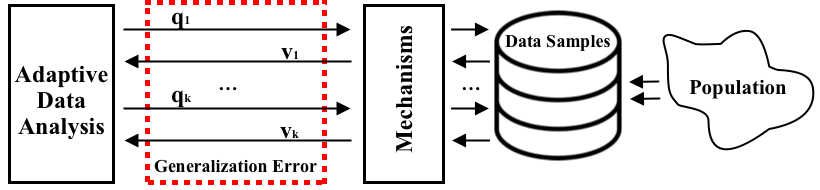
\includegraphics[width=0.7\columnwidth]{figures/data_analysis_model.png}
  \caption{Overview of our Adaptive Data Analysis model.}
  \label{fig:adaptivity-model-overview}
 \vspace{-0.5cm}
 \end{figure}
 This guarantees that the result of the queries generalizes well. 
 This approach is described in Figure~\ref{fig:adaptivity-model-overview}, where
 I have a population that I am interested in studying, and a dataset containing individual samples from this population. The adaptive data analysis I am interested in running has access to the dataset through queries of some pre-determined family (e.g., statistical or linear queries) mediated by a mechanism. 
 This mechanism uses randomization to reduce the generalization error of the queries issued to the data.
 This line of work has identified many new algorithmic techniques for ensuring generalization in adaptive data analysis, leading to algorithms with greater statistical power than all previous approaches. 
 Common methods proposed by these works include the addition of noise to the result of a query, data splitting, etc. 
 Moreover, these works have also identified problematic strategies for adaptive analysis, showing limitations on the statistical power one can hope to achieve. 
 Subsequent works have then further extended the methods and techniques in this approach and further extended the theoretical underpinning of this approach, 
 e.g.~\cite{dwork2015reusable,dwork2015generalization,BassilyNSSSU16,UllmanSNSS18,FeldmanS17,jung2019new,SteinkeZ20,RogersRSSTW20}.
 %
 
 A key development in this line of work is that the best method for ensuring generalization in an adaptive data analysis depends to a large extent on the number of \emph{rounds of adaptivity}, the depth of the chain of queries. 
 As an informal example, the program $x \leftarrow \query_1(D);y \leftarrow \query_2(D,x);z \leftarrow \query_3(D,y)$ has three rounds of adaptivity, since $\query_2$ depends on $D$ not only directly because it is one of its input but also via the result of $\query_1$, 
 which is also run on $D$, and similarly, $\query_3$ depends on $D$ directly but also via the result of $\query_2$, which in turn depends on the result of $\query_1$. 
 The works I discussed above showed that not only does the analysis of the generalization error depend on the number of rounds, 
 but knowing the number of rounds allows one to choose methods that lead to the smallest possible generalization error. 
 
 % \mg{Check the following - also the plots need to be on the same scale!}
 For example, these works showed that when an adaptive data analysis uses a large number of rounds 
 of adaptivity then a low generalization error can be achieved by the mechanism that 
 adds Gaussian noise scaled to the number of rounds to each query result.
 When instead an adaptive data analysis uses a small number of rounds of adaptivity then a low generalization error can be achieved by using more specialized methods, such as the data splitting mechanism or the reusable holdout technique from~\cite{DworkFHPRR15}.
 To better understand this idea, I show in Figure~\ref{fig:generalization_errors} two experiments showcasing these situations. 
 More precisely, in Figure~\ref{fig:generalization_errors}(a) shows the results of a real-world analysis
 with two rounds of adaptivity. 
 This analysis can be seen as a classifier that first runs 500 non-adaptive queries on the first 500 attributes of the data, looking for correlations between the attributes and a label, and then runs one last query which depends on all these correlations. 
 Without any mechanism, the generalization error is pretty large, and the lower generalization error is achieved when the data-splitting method is used. 
 In Figure~\ref{fig:generalization_errors}(b) shows the results of a specific analysis
 with four hundred rounds of adaptivity. 
 This analysis can be seen as a classifier that at each step runs an adaptive query based on the result of the previous ones. 
 Again, without any mechanism, the generalization error is pretty large, and the lower generalization error is achieved when the Gaussian noise is used. 
 {\small
 \begin{figure}
 \centering
 \begin{subfigure}{.48\textwidth}
 \begin{centering}
 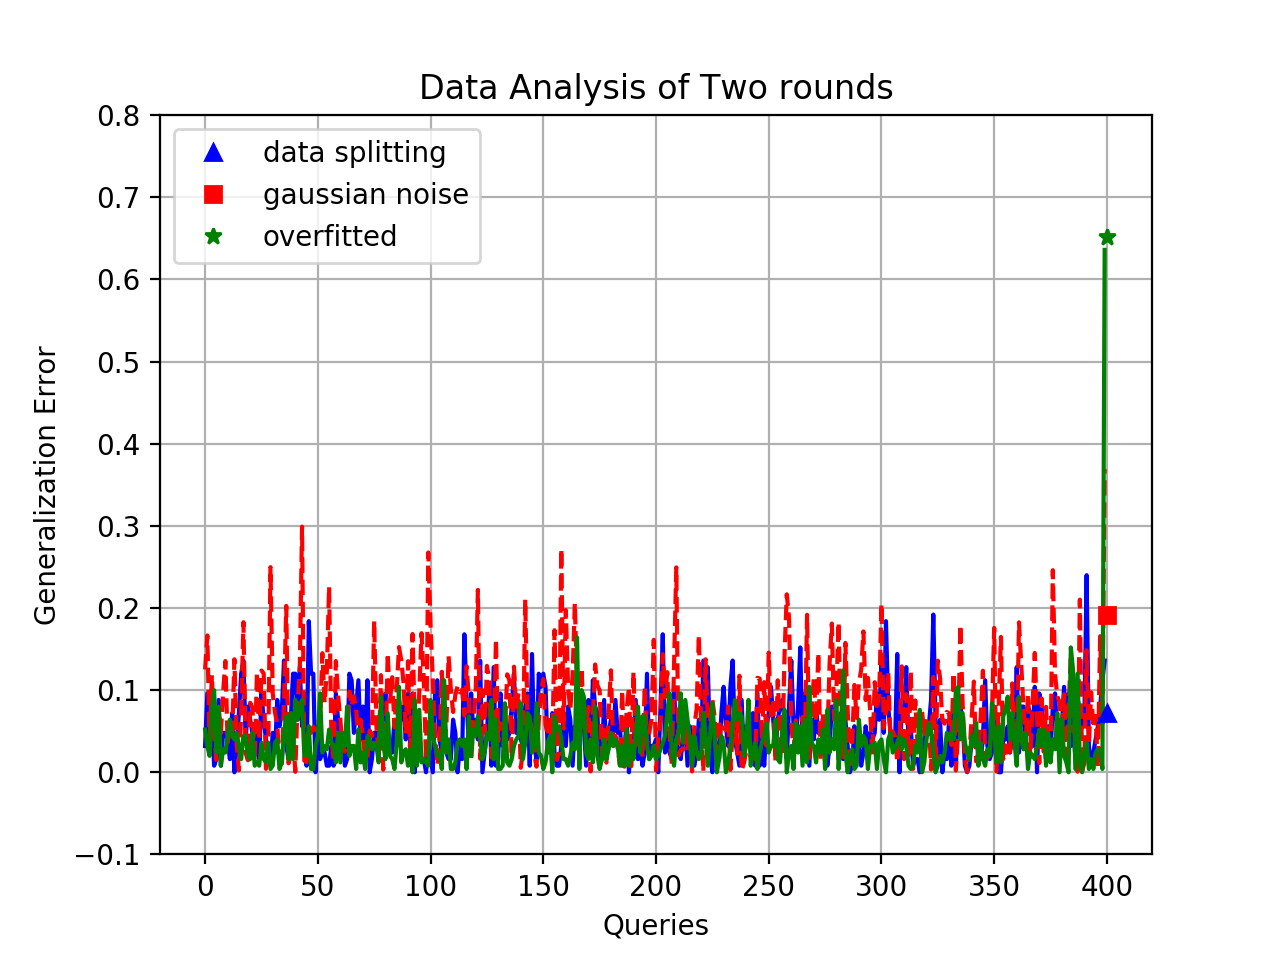
\includegraphics[width=0.9\textwidth]{figures/tworound.png}
 \caption{}
 \end{centering}
 \end{subfigure}
 %}
 \quad
 \begin{subfigure}{.48\textwidth}
 \begin{centering}
 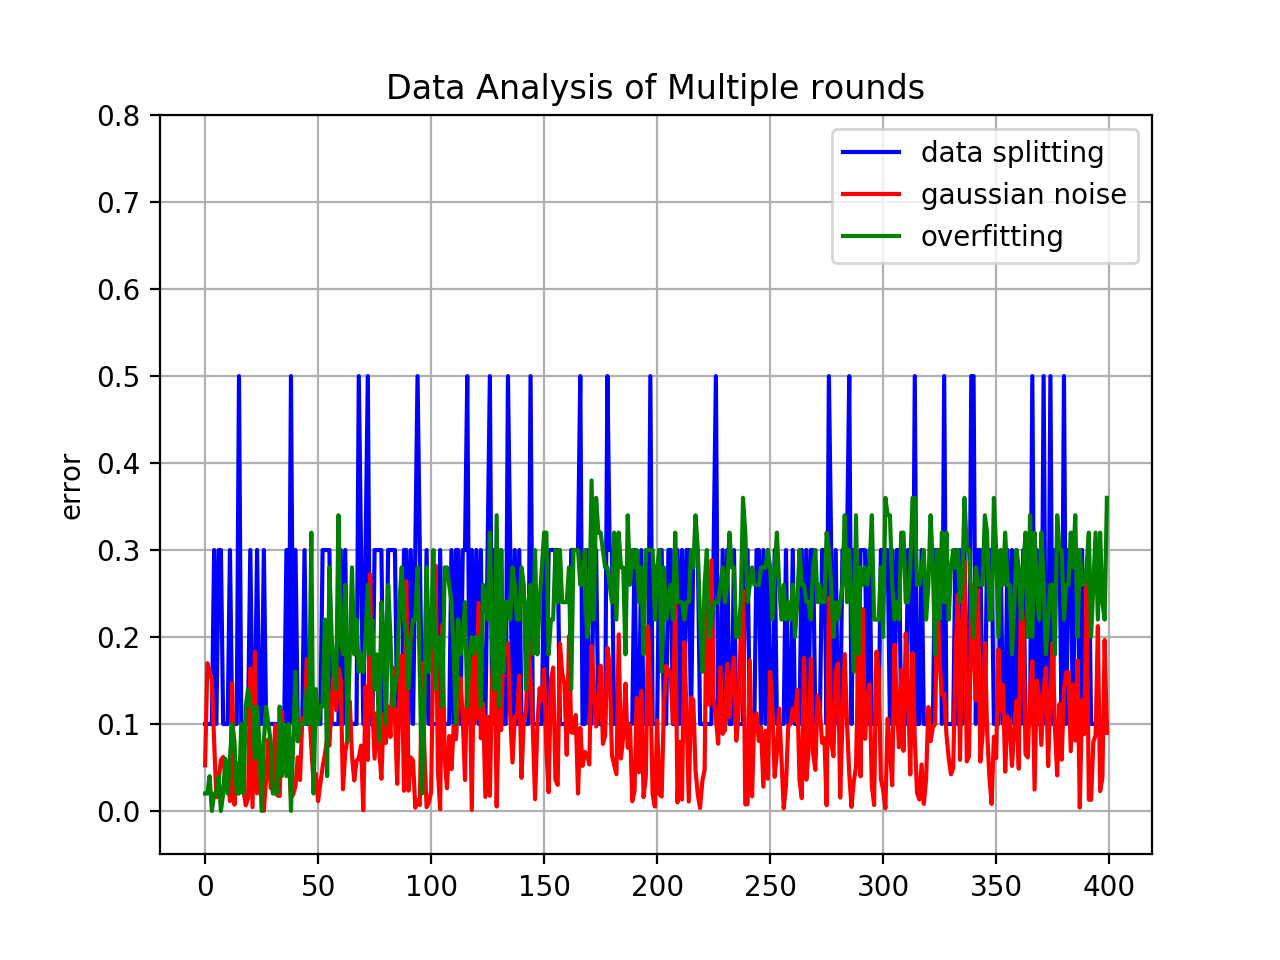
\includegraphics[width=0.9\textwidth]{figures/multipleround.png}
 \caption{}
 \end{centering}
 \end{subfigure}
 \vspace{-0.4cm}
  \caption{
  The generalization errors of two adaptive data analysis examples, under different choices of mechanisms.
  (a) Data analysis with adaptivity 2, 
  (b) Data analysis with adaptivity 400. 
 }
 \label{fig:generalization_errors}
 \vspace{-0.5cm}
 \end{figure}
 }
 %gap
 This scenario motivates us to explore the design of program analysis techniques that can be used to estimate the number of \emph{rounds of adaptivity} that a program implementing a data analysis can perform. These techniques could be used to help a data analyst in the choice of the mechanism to use,
 and they
 could ultimately be integrated into a tool for adaptive data analysis such as the \emph{Guess and Check} framework by~\cite{RogersRSSTW20}. 
 %
\subsection{Challenges}
\label{sec:adapt-challenge}
Given the significance of this \emph{adaptivity} quantity in data analysis area,
I'm motivated to analysis this property.
In order to analyze this property, there is mainly three challenges introduced below.
%  in Section~\ref{sec:adapt-intro-challenge}.
Then targeting to the three challenges, I give a short overview of the new proposed adaptivity analysis framework
with respect to the limitations of previous works.

\begin{enumerate}
 \item
 \textbf{Adaptive Data Analysis Formalization}

The first challenge is \emph{how to define formally} a model for adaptive data analysis which is general enough to support the methods I discussed above and would permit to formulate the notion of adaptivity these methods use. 
I take the approach of designing a programming framework for submitting queries to some \emph{mechanism} giving access 
to the data mediated by one of the techniques which are mentioned before, 
including the mechanism of adding Gaussian noise, 
the mechanism that randomly selects a subset of the data, 
and the mechanism that uses the reusable holdout technique, etc. 
In this approach, a program models an \emph{analyst} asking a sequence of queries to the mechanism. 
The mechanism runs the queries on the data applying one of the methods discussed above and returns the result to the program. The program can then use this result to decide which query to run next. 
% Overall, I am interested in controlling the generalization of the results of the queries which are returned by the mechanism, by means of adaptivity. 

% \textbf{Methodology}
% There are previous works from \todo{Thesis} developing language formalizing the adaptive data analysis.
% However, their formalization is limited in the expressiveness largely.
Motivated by this, I present a new while-like language 
named {\tt Query While} language with extensions on query requests in Section~\ref{sec:adapt-language}.

\item 
\textbf{Adaptivity Formalization}

The second challenge is \emph{how to define the adaptivity of a given program}.
Intuitively, a query $Q$ may depend on another query $P$, if there are two values that $P$ can return which affect in different ways the execution of $Q$. 
For example, as shown in \cite{dwork2015reusable}, and as I did in our example in Figure~\ref{fig:generalization_errors}(a), one can design a machine learning algorithm for constructing a classifier that first computes each feature's correlations with the label via a sequence of queries, and then constructs the classifier based on the correlation values. 
If one feature's correlation changes, the classifier depending on features is also affected. 
This notion of dependency builds on the execution trace as a \emph{causal history}. 
In particular, I am interested in the history or provenance of a query up until this is executed, 
% I am not then concerned about how the result is used --- except for 
simultaneously in tracking whether the result of the query may further cause some other query. 
This is because I'm focusing on the generalization error which could be propagated by queries.
% and not their post-processing. % 

To formalize this intuitive \emph{adaptivity} as a quantitative program property, 
I present an adaptivity definition in Section~\ref{sec:adapt-exe} based on the language and semantics.
% \textbf{Methodology}
% % I first consider all the possible evaluations of a program --- I do this by 
% % I use a trace semantics recording the execution history of programs on some given input --- and I create a dependency graph, where the dependency between different variables (query is also assigned to a variable) is explicit and track which variable is associated with a query request. 
% % I then enrich this graph with weights describing the maximal number of times each variable is evaluated in a program evaluation starting with an initial state. The adaptivity is then defined as the length of the walk visiting most query-related variables on this graph. 
% % Through two aspects: the execution-based analysis and static-based program analysis.
% % In the execution-based analysis, I will formalize the intuitive notion of \emph{adaptivity} as a quantitative 
% % property of programs. This analysis is developed 
%  This execution-based analysis is designed in three steps through different methodologies as follows,
%  \begin{enumerate}
%  \item The first step is to analyze the \emph{dependency relation} between every query, 
%  through the methodology of semantic data dependency analysis.
%  %
%  Specifically through a trace semantics recording the execution history of programs on given input,
%  % --- and I create a dependency graph, 
%  the dependency between different variables (query is also assigned to a variable) is explicitly tracked and 
%  analyzed.
% %   and 
% %   which variable is associated with a query request. 
% % I then enrich this graph with weights describing the maximal number of times each variable is evaluated in a program evaluation starting with an initial state. The adaptivity is then defined as the length of the walk visiting most query-related variables on this graph. 
% % In the execution-based analysis, I will formalize the intuitive notion of \emph{adaptivity} as a quantitative 
% % property of programs. This analysis is developed 
% % \\
%  \item The second step is to analyze the \emph{dependency quantity} 
% %  analysis, 
% based on the \emph{dependency relation} above.
% This analysis is developed through the methodology of execution-based reachability bound analysis.
% % \\
%  \item The last step is the intuitive \emph{adaptivity} quantity analysis, 
%  according to the two analysis results above, specifically \emph{dependency relation} and \emph{dependency quantity}.
%  This step 
% %  is developed through 
% gives the formal \emph{adaptivity} definition as the analysis result. \\
%  Specifically, this analysis is developed through creating a dependency graph firstly. 
%  In this graph, the dependency between different variables (query is also assigned to a variable) 
%  is explicit and track which variable is associated with a query request. 
%  This dependency comes from the \emph{dependency relation} from the first step analysis.
%  \\
% Then, I enrich this graph with 
% weights describing the maximal number of times each variable is evaluated in a program evaluation starting with an initial state. 
% This weight comes from the \emph{dependency quantity} from the second step analysis results.
% \\
%  The adaptivity is then defined as the length of the walk visiting most query-related variables on this graph. 
%  \end{enumerate}
\item 
\textbf{Adaptivity Estimation}

The third challenge is \emph{how to estimate the adaptivity of a given program}. 
The adaptive data analysis model I consider and our definition of adaptivity suggest that for this task 
I can use a program analysis that is based on some form of dependency analysis.
 This analysis needs to take into consideration:
1) the fact that, in general, a query $Q$ is not a monolithic block but rather it may depend, through the use of variables and values, on other parts of the program. 
Hence, it needs to consider some form of data flow analysis. 
2) the fact that, in general, the decision on whether to run a query or not may depend on some other value. Hence, 
 it needs to consider some form of control flow analysis.
3) the fact that. in general, I am not only interested in whether there is a dependency or not, but in the length of the chain of dependencies. 
Hence, it needs to consider some quantitative information about the program dependencies. % {A quick example is that: I store the result of query $Q_1$ in variable $x$ and use variable $y$ to record the result of query $Q_2$. I want to construct the third query $Q_3$ which relies on the value stored in $x$, let us say, $Q_3$ will ask for the sum of the first column of a table if $x$ is positive and the sum of the second column otherwise. In this situation, I need data flow analysis. On the other hand, if I need the value of $y$ to help us decide whether I should ask $Q_3$, for example, I ask the third query if $y$ is odd, and do not ask if $y$ is even. Naturally, to be able to handle this case, control flow analysis comes into play. Formally speaking, }

To address these considerations and be able to estimate a sound upper bound on the adaptivity of a program, 
I propose a static program analysis in Section~\ref{sec:adapt-static}, named {\THESYSTEM}.
%%%%% To reason about%
\end{enumerate}

In summary, this new program analysis framework is
%  developed
%  full-spectrum analysis of this property is 
% In this proposal, I will first focus on analyzing 
% this adaptivity property for the program based on solving 
developed w.r.t. the three challenges accordingly,
through the three parts:
the language formalization,
the formal adaptivity definition and the static program analysis algorithm estimating adaptivity.


\subsection{Outline}
\label{sec:adapt-outline}
The rest parts of this section is organized as follows. 
\begin{enumerate}
   \item The previous works on adaptive data analysis are introduced in Section~\ref{sec:prework}.
   \item The proposed new program analysis framework for the adaptivity of Adaptive Data Analysis is presented 
   in Section~\ref{sec:adapt-analysis}.
   This new program analysis framework has three major components:
   \begin{enumerate}
      \item A while-like language extended with query request feature, named {\tt Query While} Language  in Section~\ref{sec:adapt-language}, 
      used to implement the adaptive data analysis;
      \item A formal adaptivity definition in Section~\ref{sec:adapt-exe};
      \item A static program analysis algorithm, named {\THESYSTEM} through static adaptivity analysis in Section~\ref{sec:adapt-static}.
   \end{enumerate}
\end{enumerate}

\section{Previous Works on Adaptivity Analysis}
\label{sec:prework}
This chapter introduces the previous works on analyzing the adaptivity property
for adaptive data analysis and the limitation analysis.
There are mainly three parts in previous works.
Each of them focus on solving one of the challenges introduced above in analyzing the adaptivity.
In Section~\ref{sec:prework-language}, I introduce the previous language design, which aims to formalize
the adaptive data analysis program and solve the first challenge.
Section~\ref{sec:prework-formalization} summarizes the previous works
on defining this intuitive \emph{adaptivity} quantity through a formal model,
targeting on the second challenge.
Then Section~\ref{sec:prework-static} includes a summary of previous works on estimating
their formalized \emph{adaptivity} and the limitations.

\subsection{The Language Design}
\label{sec:prework-language}
Previous works formalized the adaptive data analysis into a while-like language named loop language with  limited expressiveness.
It is presented in {Thesis~\cite{weihao22}}.
\subsection*{Syntax}
Figure~\ref{fig:prework_syntax} is a selection of the syntax from their loop language.
{\small
\begin{figure}
\[
\begin{array}{llll}
    % \mbox{Values } & v & ::= & n \sep \etrue \sep \efalse \sep \chi \sep [] ~|~ [v, \dots, v] ~|~ \chi[v] \\
 \mbox{Arithmetic Operators} & \oplus_a & ::= & + ~|~ - ~|~ \times 
%
~|~ \div \\  
  \mbox{Boolean Operators} & \oplus_b & ::= & \lor ~|~ \land ~|~ \neg\\
  %
   \mbox{Relational Operators} & \sim & ::= & < ~|~ \leq ~|~ == \\  
%  \mbox{Label} & l & := & \mathbb{N} \\ 
%  \mbox{Loop Maps} & w & \in & \mbox{Label} \times \mathbb{N} \\
\mbox{Arithmetic Expressions} & \aexpr & ::= & 
	%
	n ~|~ x ~|~ \aexpr \oplus_a \aexpr  \\
% 	\sep \pi (l , \aexpr, \aexpr) \\
    %
\mbox{Boolean Expressions} & \bexpr & ::= & 
	%
	\etrue ~|~ \efalse  ~|~ \neg \bexpr
	 ~|~ \bexpr \oplus_b \bexpr
	%
	~|~ \aexpr \sim \aexpr \\
\mbox{Expressions} & \expr & ::= & \aexpr ~|~ \bexpr ~|~ [] ~|~ [\expr, \dots, \expr] \\	
\mbox{Values} & v & ::= & n ~|~ \etrue ~|~ \efalse ~|~ [] ~|~ [v, \dots, v] \\
\mbox{Query expressions} & \expr_q & ::= & \aexpr ~|~ \chi ~|~ \chi[\aexpr] ~|~ \expr_q \oplus_a \expr_q \\
\mbox{Query Values} & v_q & ::= & n ~|~ \chi ~|~ \chi[n] ~|~ v_q \oplus_a  v_q \\
% \mbox{Labelled commands} & c & ::= & 
% [\assign x \expr]^{l} ~|~  [\assign x q(e_q)]^{l}
%  ~|~  \eloop ~ [\aexpr]^{l} ~ \edo ~ c  ~|~ c;c \\
%  & & & ~|~ \eif([\bexpr]^l, c, c) 	 ~|~ [\eskip]^{l} \\
\mbox{Commands} & c & ::= &  \eskip  ~|~  \assign x \expr ~|~  \assign{x}{ q(\expr_q)}
%
~|~ \eloop ~ \aexpr  ~ \edo ~ c  \\ &&& ~|~ c;c  ~|~ \eif(\bexpr, c, c)
\end{array}
\]
 \caption{Syntax of loop language.}
    \label{fig:prework_syntax}
\end{figure}
}
The expressions can be arithmetic expressions, boolean expressions or query expression.
The arithmetic expressions boolean expressions are standard.
They extend the expression with the query expression in order to support the query requests in the data analysis.
The special variable $\chi$ represents a row of the database,
and access to values at a certain index in $\chi$, as $\chi[\aexpr]$.
But it neither  support while loop with non-deterministic iterations, nor any user input.
%
\subsection*{Trace-Based Operational Semantics}
The previous operational semantics is defined based on labeled command and trace with some special operators.
Below is a summary of their designs.
\paragraph*{Labeled Commands}
They first annotate each command with a label $l$,
a natural number standing for the line of code where the command appears.
They associate the label $l$ to the conditional predicate $\bexpr$ in the if statement,
and to the loop counter $\aexpr$ in the loop statement.
\[
\begin{array}{llll}
     \mbox{Labeled commands} & c & ::= &   [\assign x \expr]^{l} ~|~  [\assign x q(e_q)]^{l}
 ~|~  \eloop ~ [\aexpr]^{l} ~ \edo ~ c  ~|~ c;c \\
 & & & ~|~ \eif([\bexpr]^l, c, c) 	 ~|~ [\eskip]^{l} \\
\end{array}
\]
% Each command is now labeled 
\paragraph*{Loop Map}
Then, they have the Loop map, which is a map from the label $l$ to the iteration number $n$.
%   Because statements in the loop share the same line number,  varied iterations , the label $l$ is not enough to distinguish statements.
  A mapping $[k \to n]$ gives accurate information on which loop a statement is in by its key $k$ (label at loop counter),
  and which iteration $n$ the statement belongs to.
  % For example, the loop map $w=[3:1, 4:2]$ indicates that the statement is currently in a nested loop, the outer loop starting from label $3$ and in its first iteration, the statement is now in the inner loop starting from label $4$ and in the second iteration. We use $\emptyset$ to represent an empty map, indicating the statement is not in any loop.
\[
\begin{array}{llll}
 \mbox{Loop Map} & w & \in & \mbox{Label} \to \mathbb{N} \\
\mbox{Annotated Query} & \mathcal{AQ}  & ::= & \{ q(v_q)^{(l,w)}  \} \\
\end{array}
\begin{array}{llll}
    \mbox{Memory} & m & ::= & [] ~|~ m[x \to v] \\
\mbox{Trace} & t & ::= & [] ~|~ q(v_q)^{(l, w) } :: t \\
\end{array}
\]
%  Then, they have the Loop map, which is a map from the label $l$ to the iteration number $n$.
% %   Because statements in the loop share the same line number,  varied iterations , the label $l$ is not enough to distinguish statements.
%   A mapping $[k \to n]$ gives accurate information on which loop a statement is in by its key $k$ (label at loop counter),
%   and which iteration $n$ the statement belongs to.
%   % For example, the loop map $w=[3:1, 4:2]$ indicates that the statement is currently in a nested loop, the outer loop starting from label $3$ and in its first iteration, the statement is now in the inner loop starting from label $4$ and in the second iteration. We use $\emptyset$ to represent an empty map, indicating the statement is not in any loop.

 \paragraph*{Annotated Query} 
 They 
distinctively design the annotated query, in order to analyze the relation between queries. This is a key extension for analyzing the \emph{adaptivity}
Through this annotation, queries can be uniquely annotated as $\mathcal{AQ}$,
  and the annotation $(l,w)$ considers the location of the query
  by line number $l$ and which iteration the query is at when it appears in a loop statement, specified by $w$.
  %% trace
\paragraph{Trace} 
A trace $t$ is a list of annotated queries accumulated along with the execution of the program. 
%   A trace can be regarded as the program history, where this history 
  It consists of the queries asked by the analyst during the execution of the program,
%   We 
collected through
  a trace-based small-step operational semantics based on transitions of the form $ \config{m,c, t, w} \to \config{m', \eskip, t', w'} $.
  % \paragraph{Memory}
  % The memory in their language is standard, which is a map from variables to values.
  \paragraph*{Operational Semantics Rules}
Figure~\ref{fig:evaluation} is a selection of rules of their trace-based operational semantics from {Thesis~\cite{weihao22}}.
Only the rules related to query requests and the while loop evaluations are selected here.
The rule $\textbf{l-query-e}$ evaluates the argument $\expr_q$ of a query request $q(\expr_q)$ using the query evaluation $\qarrow$.
When the query expression is in the normal form, this query will be answered.
The rule $\textbf{l-query-v}$ modifies the starting memory $m$ to $m[v_q/x]$ using the answer $v$ of the query $q(v_q)$ from the mechanism, with the trace expanded by appending the query $q(v_q)$ with the current annotation $(l,w)$.
The rule for assignment is standard and the trace remains unchanged.
The sequence rule keeps tracking the modification of the trace, and the evaluation rule for if conditional goes into one branch based on the result of the conditional predicate $\bexpr$. 
The rule \textbf{l-loop-a} first evaluates the loop counter $\aexpr$, when the loop counter is a number, then the evaluation will start to execute the loop body.
The rules for loop modify the loop map $w$. In the rule $\textbf{l-loop}$, the loop map $w$ is updated by $w + l$ because the execution goes into another iteration when the condition $v_N >0$ is satisfied.
% When $v_N$ reaches $0$, the loop exits and the loop map $w$ eliminates the label $l$ of this loop statement by $w \setminus l$ in the rule $\textbf{l-loop-exit}$. 
% 
\begin{figure}
{\footnotesize
  \begin{mathpar}
  % \boxed{ \config{m, c, t,w} \xrightarrow{} \config{m', c',  t', w'} \; }
  % \\
  % \inferrule
  % {
  %  \config{m, \expr } \xrightarrow{}  \config{m, \expr' }
  % }
  % {
  % \config{m, [\assign x \expr]^{l},  t,w} \xrightarrow{} \config{m, [\assign x \expr']^{l}, t,w}
  % }
  % ~\textbf{l-assn1}
  % \and
  % %
  % \inferrule
  % {
  % }
  % {
  % \config{m, [\assign x v]^{l},  t,w} \xrightarrow{} \config{m[v/x], [\eskip]^{l}, t,w}
  % }
  % ~\textbf{l-assn2}
  % %
  % \and
  {\inferrule
  {
    \config{m, \aexpr} \aarrow \config{m, \aexpr'}
  }
  {
  \config{m, \eloop ~ [\aexpr]^{l}  ~ \edo ~ c ,  t, w }
  \xrightarrow{} \config{m, \eloop ~ [\aexpr']^{l} ~ \edo ~ c ,  t, (w + l) }
  }
  ~\textbf{l-loop-a}
  }
  %
  \and
  %
  {\inferrule
  {
    \valr_N > 0
  }
  {
  \config{m, \eloop ~ [\valr_N]^{l}  ~ \edo ~ c ,  t, w }
  \xrightarrow{} \config{m, c ;  \eloop ~ [(\valr_N-1)]^{l} ~ \edo ~ c ,  t, (w + l) }
  }
  ~\textbf{l-loop}
  }
  %
  % \and
  % %
  % {
  % \inferrule
  % {
  %   \valr_N = 0
  % }
  % {
  % \config{m,  \eloop ~ [\valr_N]^{l} ~ \edo ~ c  ,  t, w }
  % \xrightarrow{} \config{m, [\eskip]^{l} ,  t, (w \setminus l) }
  % }
  % ~\textbf{l-loop-exit}
  % }
  %
  \and
  % {  Memory \times Com  \times Trace \times WhileMap \Rightarrow^{} Memory \times Com  \times Trace \times WhileMap}
  \inferrule
  {
  \config{m,\expr_q} \qarrow \config{m,\expr_q'}
  }
  {
  \config{m, [\assign{x}{q(\expr_q)}]^l, t, w} \xrightarrow{}  \config{m, [\assign{x}{q(\expr_q')}]^l, t, w}
  }
  ~\textbf{l-query-e}
  \and
  \inferrule
  {
  q(v_q) = v
  }
  {
  \config{m, [\assign{x}{q(v_q)}]^l, t, w} \xrightarrow{} \config{m[ v/ x], \eskip,  t \mathrel{++} [q(v_q)^{(l,w )}],w }
  }
  ~\textbf{l-query-v}
  %
  \and
  %
  %
  % \inferrule
  % {
  % \config{m, c_1,  t,w} \xrightarrow{} \config{m', c_1',  t',w'}
  % }
  % {
  % \config{m, c_1; c_2,  t,w} \xrightarrow{} \config{m', c_1'; c_2, t',w'}
  % }
  % ~\textbf{l-seq1}
  % %
  % \and
  % %
  % \inferrule
  % {
  % }
  % {
  % \config{m, [\eskip]^{l} ; c_2,  t,w} \xrightarrow{} \config{m, c_2,  t,w}
  % }
  % ~\textbf{l-seq2}
  % %
  % %
  % \and
  % %
  % \inferrule
  % {
  % \config{ m, \bexpr} \barrow \bexpr'
  % }
  % {
  % \config{m, \eif([\bexpr]^{l}, c_1, c_2),  t,w} 
  % \xrightarrow{} \config{m,  \eif([\bexpr']^{l}, c_1, c_2),  t,w}
  % }
  % ~\textbf{l-if}
  % %
  % \and
  %
  % \inferrule
  % {
  % }
  % {
  % \config{m, \eif([\etrue]^{l}, c_1, c_2),t,w} 
  % \xrightarrow{} \config{m, c_1,  t,w}
  % }
  % ~\textbf{l-if-t}
  % \and
  % %
  % \inferrule
  % {
  % }
  % {
  % \config{m,  \eif([\efalse]^{l}, c_1, c_2),  t,w} 
  % \xrightarrow{} \config{m, c_2,  t,w}
  % }
  % ~\textbf{l-if-f}
  %
  % %
  %
  \end{mathpar}
  }
        \caption{Trace-based operational semantics of loop language.}
        \label{fig:evaluation}
    \end{figure}
    %
    % explanation of rules
 \highlight{
\paragraph*{Limitations of The Trace-Based Operational Semantics}
This operational semantics is limited in the following aspects:
\begin{itemize}
 \item \textbf{Expressiveness Limitation}
 \\
 The operational-semantics causes a similar limitation as their syntax.
 The loop iteration number can only be a constant number or an arithmetic expression evaluated to a nature number.
 This is caused by their operational semantics rule design, trace design, and their annotated query design.
 In the rule \rname{l-loop}, a nature number $v_N$ is required on the premise of tracking the iteration times.
 This requires that the loop iteration number has to be a nature number or evaluated to a nature number in advance to execute the loop.
 Then in their trace and annotated query design,
 % generated through the operational semantics rules.
 the trace tracks the annotated query, which requires an integer annotation explicitly indicating the iteration number of the loop.
 % annotatation of the the query request executed in the program
 % with integer indicating the while loops. 
 \\
 For example, in the following program with a simple while loop,
 \[
 {\assign{x}{20}};
 \assign{y}{100};
 \ewhile (x < y) \edo 
 \{
 \assign{x}{x + 1};
 \assign{y}{y - 2};
 \}\}
 \] 
 the number of iterations cannot be evaluated to a nature number in advance of entering this loop. 
 The iteration number is only
 able to be decided during executing this while loop body.
 This program represents a class of data analysis programs with non-constant loop iterations
 which is very common in data analysis. However, it isn't supported by their design.
 \item \textbf{Accuracy Limitation}
 \\
 This operational semantics design causes in-precision in formalizing the \emph{adaptivity}.
 Because there is information loss in their trace generated through the operational semantic rules.
 The trace only tracks the query requests. This lost the information of the variables
 which are assigned by query values even if they are not assigned by query requests. However, these variables
 are critical in analyzing the \emph{adaptivity}.
 This will be analyzed in detail in the limitation in Section~\ref{sec:prework-formalization}.
 \item \textbf{Efficiency Limitation}
 \\
 There are four components in their configuration in order to evaluate the program. 
 The update operations for this quadruple configuration are low-efficient, especially the update operation of the while map.
\end{itemize}
}   
%
\subsection{The Adaptivity Definition}
\label{sec:prework-formalization}
The previous works on formalizing the adaptivity is through a query-based dependency graph.
Below is a summary of their query-based dependency graph construction and adaptivity formal definition, followed
by the weaknesses of this formalization method.
\subsection*{Query-Based Dependency Graph}
They build their dependency graph over annotated queries, in order to construct the edge between queries for this graph, they first
define a query \emph{May-Dependency} relation. Below is a summary of this definition from
% Below is the formal definition of query may dependency based on their trace-based operational semantics 
from Thesis~\cite{weihao22}.
The notations $\in_q$ and $\not\in_q$ a query belongs to the trace or not respectively, with the full details in Thesis~\cite{weihao22}.
\begin{defn}[Query may dependency]
One query $q({v_q}_1)$ may depend on another query $q({v_q}_2)$ in a program $c$, with a starting loop maps $w$, a starting memory $m$, hidden database $D$, denoted as \\
$\mathsf{DEP}(q({v_q}_1)^{(l_1, w_1)}, q({v_q}_2)^{(l_2, w_2)}, c,w, m, D)$ is defined below. 
\[
  {\footnotesize
\begin{array}{l}
\forall  t. \exists m_1,m_3,t_1,t_3,c_2.\\
  \left (\begin{array}{l}   
\config{m, c,  t,w} \rightarrow^{*} \config{m_1, [\assign{x}{q({v_q}_1)}]^{l_1} ; c_2,
  t_1,w_1} \rightarrow \\ \config{m_1[q({v_q}_1)(D)/x], c_2,
  t_1++[q({v_q}_1)^{(l_1, w_1)}], w_1} \rightarrow^{*} \config{m_3, \eskip,
  t_3,w_3} \\  
  \land \\
\Big( q({v_q}_1)^{(l_1,w_1)} \in_{q} (t_3-t) \land q({v_q}_2)^{(l_2,w_2)} \in_{q} (t_3-t_1) \\ \implies  \exists v \in \codom(q({v_q}_1)), m_3', t_3', w_3'.  \\
 \config{m_1[v/x], {c_2}, t_1++[q({v_q}_1)^{(l_1,w_1)}], w_1} \rightarrow^{*} \config{m_3', \eskip, t_3', w_3'} \\ \land (q({v_q}_2)^{(l_2,w_2)}) \not \in_{q} (t_3'-t_1)
\Big)\\
\land \\
\Big(q({v_q}_1)^{(l_1,w_1)} \in_{q} (t_3-t) \land q({v_q}_2)^{(l_2,w_2)} \not\in_{q} (t_3-t_1) \\ \implies  \exists v \in \codom(q({v_q}_1)),  m_3', t_3', w_3'. \\
 \config{m_1[v/x], {c_2}, t_1++[q({v_q}_1)^{(l_1,w_1)}], w_1} \rightarrow^{*} \config{m_3', \eskip, t_3', w_3'} \\ \land (q({v_q}_2)^{(l_2,w_2)})  \in_{q} (t_3'-t_1)
\Big)
\end{array} \right )
\end{array}
}
\]
\end{defn}
%
Based on the \emph{may-dependency} between the two queries above,
below is their formal definition of query-based dependency graph. 
For every execution of a program $c$ staring with a certain memory and while map
%  configurations, 
they construct a corresponding dependency graph.  
% graph definition
\begin{defn}[Query-based Dependency Graph]
Given a program $c$, a database $D$, a starting memory $m$, an initial loop map $w$, the query-based dependency graph $G(c,D,m,w) = (V, E)$ is defined as: \\
$V =\{q({v_q})^{l,w} \in \mathcal{AQ} \mid \forall t. \exists m',  w', t'.  \config{m ,c, t, w}  \to^{*}  \config{m' , \eskip, t', w' }  \land q({v_q})^{l,w} \in {(t'-t)}  \}$.
\\
$E = \left\{(q({v_q})^{(l,w)},q({v_q}')^{(l',w')}) \in \mathcal{AQ} \times \mathcal{AQ} 
~ \left \vert ~ \mathsf{DEP}(q({v_q}')^{(l',w')},q({v_q})^{(l,w)}, c,w,m,D)
 \right.\right\}$.
\end{defn}
%
% The function $\mathsf{To}(q(v')^{(l',w')}, q(v)^{(l,w)}$ tells that the query request $q(v')^{(l',w')}$ appears after the query request $q(v)^{(l,w)}$ in the trace, by comparing the annotation $(l',w')$ and $(l,w)$. It helps to decide on the direction of one edge.
The edge is directed, when an annotated query $q({v_q})^{(l,w)}$ may depend on its previous query $q({v_q}')^{(l',w')}$, we have the directed
edge $(q({v_q})^{(l,w)}, q({v_q}')^{(l'.w')})$, from $q({v_q})^{(l,w)} $ to $q({v_q}')^{(l'.w')}$.

The query-based dependency graph only considers the newly generated annotated queries during the execution of the program $c$,
so they see the nodes coming from the trace $t'-t$.
The previous trace before the execution of $c$ is excluded when constructing the graph.
% To summarize, for every execution of a program $c$ staring with different configurations, 
% they can construct a corresponding dependency graph. 

\subsection*{Adaptivity Formalization}
Below is the definition of adaptivity from Thesis~\cite{weihao22}, by means of the query-based dependency graph. 
\begin{defn}[Adaptivity in {loop} language]
Given a program $c$, and a memory $m$, a database $D$, a starting loop map $w$, the adaptivity of the dependency graph $G(c, D,m,w) = (V, E)$ is the length of the longest path in this graph. We denote the path from $q({v_q})^{(l,w)}$ to $q({v_q}')^{(l',w')}$ as $p(q({v_q})^{(l,w)}, q({v_q}')^{(l',w')} )$. The adaptivity denoted as $A(c, D, m, w)$.
%
$$A(c, D, m, w) = \max\limits_{q({v_q})^{(l,w)},q({v_q}')^{(l',w')} \in V } |p(q({v_q})^{(l,w)}, q({v_q}')^{(l',w')} )| $$
\end{defn}
\subsection*{Limitations}
Limited by their language design and the dependency graph construction,
this adaptivity definition is weak in the following aspects.
\highlight{
 \begin{enumerate}
 \item \textbf{Expressiveness Limitation}
 \\
 The definition isn't general enough to give the formal adaptivity for the adaptive data analysis programs with non-constant
 while loops.
 However, programs containing while loops of non-deterministic iteration times are very common in the adaptive data analysis area.
 This is caused by the expressiveness limitation in their language design and operational semantics design as analyzed
 in Section~\ref{sec:prework-language}.
 \\
 In the following example program similar to the one in Section~\ref{sec:prework-language} with two extra query request commands,
 \[
 {\assign{x}{0}};
 \assign{y}{5};
 \assign{z}{q(x + y)};
 \ewhile (x < y) \edo 
 \{
 \assign{x}{x + 1};
 \assign{y}{y - 1};
 \assign{z}{q(x+y+z)};
 \}\}
 \] 
 the number of iterations cannot be evaluated to a nature number in advance of entering this loop for the same reason. 
 The iteration number is only
 able to be decided during executing this while loop body.
 % This program represents a class of data analysis programs with non-constant loop iterations, which is very common in data analysis. However, it isn't supported by their design.
 \\
 Limited by this, they cannot give the adaptivity for this program even though the adaptivity in this program is 4, which is straightforward to observe.
 % a trace generated for this program
 \item \textbf{Accuracy Limitation}
 \\
 The in-accuracy of this \emph{adaptivity} definition is caused by both their language design and their graph construction.
 \\
 As analyzed in Section~\ref{sec:prework-language}, the information in non-query requesting variables are lost.
 The dependency that passes through these variables is lost, and the adaptivity is lost as well.
 \\
 The other reason for this in-accuracy comes from their graph definition.
 This dependency graph definition relies on a specific memory, while-map, and a specific execution trace.
 It limits the adaptivity defined for the adaptive data analysis program to be w.r.t. one specific
 execution.
 In the other words, this adaptivity definition doesn't correspond to the \emph{adaptivity} for this program,
 but for the program in a certain execution.
 % to The trace only tracks the query requests. This lost the information of the variables
 % which are assigned by query values even if they are not assigned by query requests. 
 \item \textbf{Efficiency Limitation}
 \\
 This definition is in-efficient in the sense that it requires the full unfolding of every iteration for the while loop.
 There are two reasons for this unfolding operation.
 The first one comes from the low efficiency of their trace-based operational semantics,
 which requires the trace to track the loop iteration number in the annotated query.
 The other comes from their dependency graph generation, which requires every query request evaluated during the program execution
 as the graph nodes.
 Both of the two processes generate unnecessary and duplicate nodes during the while iterations.
 % annotatation of the the query request executed in the program
 % with integer indicating the while loops. 
\end{enumerate}
}This operational semantics is limited in the following aspects:
\begin{itemize}
 \item \textbf{Expressiveness Limitation}
 \\
 The operational-semantics causes a similar limitation as their syntax.
 The loop iteration number can only be a constant number or an arithmetic expression evaluated to a nature number.
 This is caused by their operational semantics rule design, trace design, and their annotated query design.
 In the rule \rname{l-loop}, a nature number $v_N$ is required on the premise of tracking the iteration times.
 This requires that the loop iteration number has to be a nature number or evaluated to a nature number in advance to execute the loop.
 Then in their trace and annotated query design,
 % generated through the operational semantics rules.
 the trace tracks the annotated query, which requires an integer annotation explicitly indicating the iteration number of the loop.
 % annotatation of the the query request executed in the program
 % with integer indicating the while loops. 
 \\
 For example, in the following program with a simple while loop,
 \[
 {\assign{x}{20}};
 \assign{y}{100};
 \ewhile (x < y) \edo 
 \{
 \assign{x}{x + 1};
 \assign{y}{y - 2};
 \}\}
 \] 
 the number of iterations cannot be evaluated to a nature number in advance of entering this loop. 
 The iteration number is only
 able to be decided during executing this while loop body.
 This program represents a class of data analysis programs with non-constant loop iterations
 which is very common in data analysis. However, it isn't supported by their design.
 \item \textbf{Accuracy Limitation}
 \\
 This operational semantics design causes in-precision in formalizing the \emph{adaptivity}.
 Because there is information loss in their trace generated through the operational semantic rules.
 The trace only tracks the query requests. This lost the information of the variables
 which are assigned by query values even if they are not assigned by query requests. However, these variables
 are critical in analyzing the \emph{adaptivity}.
 This will be analyzed in detail in the limitation in Section~\ref{sec:prework-formalization}.
 \item \textbf{Efficiency Limitation}
 \\
 There are four components in their configuration in order to evaluate the program. 
 The update operations for this quadruple configuration are low-efficient, especially the update operation of the while map.
\end{itemize}
%
\subsection{The Adaptivity Estimation}
\label{sec:prework-static}
In the previous works on estimating the adaptivity, they design a program analysis framework
through constructing a variable-based weighted dependency graph for
estimating the query-based dependence graph in Section~\ref{sec:prework-formalization}.
% Before they analyze and generate this graph, 
% In order to improve the analysis accuracy,
They first re-write the program from the loop language into
a Static Single Assignment (SSA) version of loop language, then estimate the adaptivity than program analysis algorithm.
% This can improve the accuracy in the variable re-assigning cases.
% The following parts summarize the SSA version of the loop language with their program analysis framework,
% followed by the limitations of their analysis method.
\subsection*{SSA-Language}
In order to distinguish different query requests in the case where they are assigned to
%  the issue of re-assignment of query requesting results to 
the same variable, they re-write the program from the loop language into SSA form.
% The SSA labeled command $\ssa{c}$ inherits from the {loop} language, except that the expressions and variables in these commands 
A selection of the (SSA) version of loop language syntax is shown below.
%  now in its SSA version as shown below. 
\[
\begin{array}{llll}
 & \ssa{c} & ::= &   [\assign {\ssa{x}}{ \ssa{\expr}}]^{l} ~|~  [\assign {{\ssa{x}} } {q({\ssa{e_q}})}]^{l}
%
~|~  {{ifvar(\bar{\ssa{x}}, \bar{\ssa{x}}')}}  ~|~ [\eskip]^{l}  ~|~
 \eloop ~ [{\ssa{\aexpr}}]^{l}, {n},  [\bar{\ssa{x}}, \bar{\ssa{x_1}}, \bar{\ssa{x_2}}] ~ \edo ~ {\ssa{c}}  ~|~ \\ &&& \ssa{c};\ssa{c}  ~|~  \eif([\ssa{\bexpr}]^{l}, ([\bar{\ssa{x}}, \bar{\ssa{x_1}}, \bar{\ssa{x_2}}] , [\bar{\ssa{y}}, \bar{\ssa{y_1}}, \bar{\ssa{y_2}}],[\bar{\ssa{z}}, \bar{\ssa{z_1}}, \bar{\ssa{z_2}}] ) , \ssa{c}, \ssa{c}) 	
\end{array}
\]
In this SSA version, if command contains the extra part $([\bar{\ssa{x}}, \bar{\ssa{x_1}}, \bar{\ssa{x_2}}] ,
[\bar{\ssa{y}}, \bar{\ssa{y_1}}, \bar{\ssa{y_2}}],[\bar{\ssa{z}}, \bar{\ssa{z_1}}, \bar{\ssa{z_2}}] )$,
which helps to track the dependency of new assigned variables in both branches($[\bar{\ssa{x}}, \bar{\ssa{x_1}}, \bar{\ssa{x_2}}]$),
then branch $[\bar{\ssa{y}}, \bar{\ssa{y_1}}, \bar{\ssa{y_2}}]$, and else branch $[\bar{\ssa{z}}, \bar{\ssa{z_1}}, \bar{\ssa{z_2}}] $. 
% The $\bar{\ssa{x}}$ is a list of SSA variables,
% in which every element $\ssa{x}$ may depend on the corresponding element(at same location),
% $\ssa{x_1}$ from $\bar{\ssa{x_1}}$ collected in the then branch or the corresponding element $\ssa{x_2}$ from $\bar{\ssa{x_2}}$ collected in the else branch.
% The size of these three lists are required to be the same.
And the loop command also has similar part $ [\bar{\ssa{x}}, \bar{\ssa{x_1}}, \bar{\ssa{x_2}}]$ focusing on the loop body.

Then they transform the operational semantics rules with all the operations defined under the loop language introduced in Section~\ref{sec:prework-language}.
Based on the transformed language, they also redefine the formal adaptivity for the transformed program equivalent to the
loop language-based definition. The complete definition is in Thesis~\cite{weihao22}.
%
\subsection*{Program Analysis Algorithm}
Then they estimate the adaptivity for a program based on rewriting it into SSA form.
This part summarizes
%  the previous analysis algorithm for estimating the adaptivity for a program. 
their analysis algorithm.
It is based on the SSA version of the loop language, and
consists of three auxiliary algorithms:
a variable estimation algorithm $\mathsf{VE}$, a matrix-vector based graph generating algorithm $\mathsf{GG}$ to generate the weighted variable-based dependency graph, and a path-searching algorithm $\mathsf{PS}$ to find the most weighted path in the graph.
%
\begin{enumerate}
    \item \textbf{{Variable Estimation Algorithm}}
\\
%
The $\mathsf{VE}$ specifies the nodes of their variable-based dependency graph. The result of $\mathsf{VE}$ is stored in a global variable list $G$, fed to the next step.
% \\
    Figure~\ref{fig:prework-static_ag1} is a selection of the three key rules from their $\mathsf{VE}$ algorithm. 
    This algorithm adds all the program variables in its SSA form to the global variable list $G$.
    % $\mathsf{VE}$ has the form $\ag{G; w; \ssa{c}}{ G'; w'} $, as shown in . The input of $\mathsf{VE}$ is a list of annotated variables $G$ collected before the program $\ssa{c}$, a loop map $w$ consistent with previous estimation, and an input SSA program $\ssa{c}$. The output of the algorithm is the updated global list $G'$, along with the updated loop maps $w$, for later estimation.  
    \\
\highlight{
    Their variable estimation for the while loop is low-efficient. As shown in rule \textbf{ag-loop},
    they unfold every iteration of the while loop, and create new annotated variables for every iteration.
    This rule causes a major efficiency limitation of their static analysis.
    It also causes a critical expressiveness limitation. By the premise in the rule \textbf{ag-loop},
    the arithmetic expression is required to be a natural number.
    This rule limits the program cannot even
    have loop with arithmetic expression like $10 + 4$ in the guard.}
\begin{figure}
{\footnotesize
 \begin{mathpar}
% \inferrule
% {
% }
% { \ag{G ;w; \ssa{[\assign {x}{\expr}]^{l}}}{G ++ [\ssa{x}^{(l,w)}];w}
% % G ;w; \ssa{[\assign {x}{\expr}]^{l}} \to G ++ [x^{(l,w)}];w 
% }
% ~\textbf{ag-asgn}
% \and
\inferrule
{
}
{ \ag{G ;w;  [ \assign{\ssa{x}}{q(\ssa{\expr_q})}]^{l}}{  G ++ [\ssa{x}^{(l,w)}] ; w} 
}~\textbf{ag-query}
%
\and 
%
\inferrule
{
\ag{G; w; \ssa{c_1}}{  G_1;w_1}
\and 
 \ag{G_1;w ; \ssa{c_2}}{  G_2; w_2}
 \\
 {G_3 = G_2 ++ \ssa{[\bar{x}^{(l,w)}]++ \ssa{[\bar{y}^{(l,w)}]}++ \ssa{[\bar{z}^{(l,w)}]} }}
}
{
\ag{G; w;
[\eif(\ssa{\bexpr},[ \bar{\ssa{x}}, \bar{\ssa{x_1}}, \bar{\ssa{x_2}}] ,[ \bar{\ssa{y}}, \bar{\ssa{y_1}}, \bar{\ssa{y_2}}],[ \bar{\ssa{z}}, \bar{\ssa{z_1}}, \bar{\ssa{z_2}}], \ssa{ c_1, c_2)}]^{l} }{ G_3 ;w}
}~\textbf{ag-if}
\and 
\inferrule
{
{G_0 = G \quad w_0 =w }
\and
\forall 0 \leq z < N. 
{ \ag{ G_z ++ \ssa{[\bar{x}^{(l, {w_z}+l)}]} ; (w_z+l); \ssa{c}}{ G_{z+1} ; w_{z+1}}  }
\\
{G_f = G_N ++ \ssa{[\bar{x}^{(l, w_N \setminus l)}]} }
\and
{ \ssa{\aexpr} =  {N}  }
}
{\ag{G; w; [\eloop ~ \ssa{\aexpr}, n, [\bar{\ssa{x}}, \bar{\ssa{x_1}}, \bar{\ssa{x_2}}] ~ \edo ~ \ssa{c}]^{l} }{ G_f; w_N\setminus l }
}~\textbf{ag-loop}
\end{mathpar}
}
 \caption{The key rule of variable estimation algorithm.  }
    \label{fig:prework-static_ag1}
\end{figure}
%
\item \textbf{Graph Generating}
\\
The algorithm $\mathsf{GG}$ generates a matrix-vector-based graph for the program. 
The matrix $M$ records the may-dependency between annotated variables in the global list $G$. It has size $|G| \times |G|$. The vector $V$ has the same size as $G$ and gives a weight to each variable in $G$.
This weight is $1$ when the variable is assigned with a query request and $0$ otherwise. 
% To be precise, the $i$th row, $j$th column of the matrix $M$, written $M[i][j]$, is  $1$ when there may be a dependency from variable $ G[i]$ to $G[j]$. Dually, $M[i][j] =0$ means no dependency. In a similar way, $V[i]=1$ means the variable $G[i]$ is assigned with a query request.
% Figure~\ref{fig:prework-static_alg2} shows some selected rules of this algorithm.
\highlight{The same key rules is selected in Figure~\ref{fig:prework-static_alg2}.
The rule \textbf{ad-loop} is as low-efficient and expressiveness-limited as the rule \textbf{ag-loop} in Figure~\ref{fig:prework-static_ag1} for the same reason.
This will be analyzed in detail in the limitation part.
}
%
\begin{figure}
{\footnotesize
\begin{mathpar}
% \inferrule
% {M = \mathsf{L}(i) * ( \mathsf{R}(\ssa{\expr},i) + \Gamma )
% }
% {
%  \gp{\Gamma;[\assign {\ssa{x}}{\ssa{\expr}} ]^{l}; i }{M; V_{\emptyset}; i+1 }
% % \Gamma \vdash_{M, V_{\emptyset}}^{(i, i+1)} [\assign {\ssa{x}}{\ssa{\expr}} ]^{l}
% }
% ~\textbf{ad-asgn}
% \and
\inferrule
{M = \mathsf{L}(i) * ( \mathsf{R}(\ssa{\expr_q},i) + \Gamma )
\\
V= \mathsf{L}(i)
}
{ 
\gp{\Gamma;[ \assign{\ssa{x}}{q(\ssa{\expr_q})} ]^{l} ; i }{M;V;i+1}
%  \vdash^{(i, i+1)}_{M, V} [ \assign{\ssa{x}}{q(\ssa{\expr})} ]^{l} 
}~\textbf{ad-query}
%
\and 
%
\inferrule
{
{\gp{\Gamma + \mathsf{R}(\ssa{\bexpr}, i_1); \ssa{c_1} ; i_1 }{ M_1;V_1;i_2 }}
% \Gamma + \mathsf{R}(\bexpr, i_1) \vdash^{(i_1, i_2)}_{M_1, V_1} \ssa{c_1} 
% : \Phi \land \bexpr \Rightarrow \Psi
\\
{\gp{\Gamma + \mathsf{R}(\ssa{\bexpr}, i_1);\ssa{c_2} ; i_2 }{ M_2; V_2 ;i_3}}
% \Gamma + \mathsf{R}(\ssa{\bexpr}, i_1) \vdash^{(i_2, i_3)}_{M_2, V_2} \ssa{c_2} 
% : \Phi \land \neg \bexpr \Rightarrow \Psi
\\
% { \forall 0 \leq j < |\bar{x}|. \bar{x}(j) = x_j, \bar{x_1}(j) = x_{1j}, \bar{x_2}(j) = x_{2j}  }
{\gp{\Gamma; [ \bar{\ssa{x}}, \bar{\ssa{x_1}}, \bar{\ssa{x_2}}]; i_3 }{ M_x; V_{\emptyset}; i_3+|\bar{\ssa{x}}| }}
%
\\\\
%
{\gp{\Gamma; [ \bar{\ssa{y}}, \bar{\ssa{y_1}}, \bar{\ssa{y_2}}]; i_3+|\bar{\ssa{x}}| }{ M_y; V_{\emptyset}; i_3+|\bar{\ssa{x}}|+|\bar{\ssa{y}}| }}
%
\\
%
{\gp{\Gamma; [ \bar{\ssa{z}}, \bar{\ssa{z_1}}, \bar{\ssa{z_2}}]; i_3+|\bar{\ssa{x}}|+ |\bar{\ssa{y}}|}{ M_y; V_{\emptyset}; i_3+|\bar{\ssa{x}}|+|\bar{\ssa{y}}| + |\bar{\ssa{z}}| }}
\\
{M = (M_1+M_2)+ M_x+M_y +M_z }
}
{
\gp{\Gamma ; \eif([\ssa{\bexpr}]^{l},[ \bar{\ssa{x}}, \bar{\ssa{x_1}}, \bar{\ssa{x_2}}] ,[ \bar{\ssa{y}}, \bar{\ssa{y_1}}, \bar{\ssa{y_2}}] , [ \bar{\ssa{z}}, \bar{\ssa{z_1}}, \bar{\ssa{z_2}}] , \ssa{ c_1, c_2)} ; i_1}{ M ;V_1 \uplus V_2  ; i_3+|\bar{x}|+|\bar{y}|+|\bar{z}| }
}
~\textbf{ad-if}
\and
% \and 
\inferrule
{
B= |\ssa{\bar{x}}| \and {A = |\ssa{c}|}
% \and
% {\Gamma \vdash^{(i, i+B)}_{M_{10}, V_{10}} [\bar{\ssa{x}}, \bar{\ssa{x_1}}, \bar{\ssa{x_2}}] }
% \and
% {\Gamma \vdash^{(i+B,i+B+A )}_{M_{20}, V_{20}} \ssa{c} 
% }
\\
\forall 0 \leq j < N. 
{\gp{\Gamma;[\bar{\ssa{x}}, \bar{\ssa{x_1}}, \bar{\ssa{x_2}}]; i+ j*(B+A) }{M_{1j};V_{1j}; i+B+j*(B+A) }}
% {\Gamma \vdash^{(i+j*(B+A), i+B+j*(B+A))}_{M_{1j}, V_{1j}}  } [\bar{\ssa{x}}, \bar{\ssa{x_1}}, \bar{\ssa{x_2}}]
\\
{
\gp{\Gamma;\ssa{c} ; i+B+j*(B+A)  }{M_{2j}; V_{2j}; i+B+A+j*(B+A) }
% \Gamma \vdash^{(i+B+j*(B+A),i+B+A+j*(B+A) )}_{M_{2j}, V_{2j}} \ssa{c} 
% : \Phi \land e_n = \lceil{z+1}\rceil \Rightarrow \Psi 
}
\\
{
\gp{\Gamma ; [\bar{\ssa{x}}, \bar{\ssa{x_1}}, \bar{\ssa{x_2}}] ; i+N*(B+A) }{M; V ;i+N*(B+A)+B}
% \Gamma \vdash^{(i+N*(B+A) ,i+N*(B+A)+B )}_{M, V} [\bar{\ssa{x}}, \bar{\ssa{x_1}}, \bar{\ssa{x_2}}]
% : \Psi \Rightarrow \Phi \land e_N = \lceil{z}\rceil 
}
\\
{ \ssa{\aexpr} =  {N}  }
\and
{M' = M+ \sum_{0 \leq j <N}( M_{1j}+M_{2j})  }
\and
{V' = V \uplus \sum_{0 \leq j <N}( V_{1j} \uplus V_{2j})  }
}
{
\gp{\Gamma;\eloop ~ [\ssa{\aexpr}]^{l}, ~0, [\bar{\ssa{x}}, \bar{\ssa{x_1}}, \bar{\ssa{x_2}}] ~ \edo ~ \ssa{c}, i }{ M';V' ;i+N*(B+A)+B }
%  \vdash^{(i,   )}_{M', V'} 
% : \Phi \land \expr_N = \lceil { N} \rceil \Rightarrow \Phi \land \expr_N = \lceil{0}\rceil
}~\textbf{ad-loop}
\end{mathpar}
}
    \caption{The key rules of the graph generating algorithm.}
    \label{fig:prework-static_alg2}
\end{figure}
%
\item \textbf{Longest Weighted Path Search}
\\
They use standard longest path search algorithm to compute the adaptivity bound over the variable-based dependency graph.
\end{enumerate}
\subsection*{Limitations}
\highlight{
\begin{enumerate}
    \item  \textbf{Efficiency Limitations}
    \begin{enumerate}
    \item
    In order to address the issue of re-assignment of different query requesting results to the same variable, they re-write the program from the loop language into SSA form.
    However, this rewriting is low-efficient and unnecessary.
    The re-assignment problem can be resolved efficiently and accurately through many state-of-art static program analysis techniques, such as the
    variable reachable analysis, etc..
    \item  Their variable estimation algorithm is low-efficient by their \textbf{ag-loop} rule in Figure~\ref{fig:prework-static_ag1},
    and rule \textbf{ad-loop} in Figure~\ref{fig:prework-static_alg2}.
    These two rules unfold every iteration of the while loop, and create new annotated variables for every iteration.
    This operation increased the complexity of the program analysis by exponential factors. 
    \item For the same reason as above, their \textbf{Graph Generation} algorithm is low-efficient as well.
    \end{enumerate}
    %
    \item \textbf{Expressiveness Limitations}
    \begin{enumerate}
    \item Their variable estimation algorithm is unable to analyze the programs with
    non-constant (or non-deterministic) loop iteration numbers.
    This is caused by their \textbf{ag-loop} rule in Figure~\ref{fig:prework-static_ag1}.
    This rule unfolds every iteration of the while loop, and create new annotated variables for every iteration.
    In order to guarantee the termination of the analysis, they have to limit the loop with constant number of loop iteration.
    Specifically in rule \textbf{ag-loop} and \textbf{ad-loop},
    % Their variable estimation for the while loop is low-efficient. As shown in rule \textbf{ag-loop},
    % they unfold every iteration of the while loop, and create new annotated variables for every iteration.
    % This rule causes a major efficiency limitation of their static analysis.
    % It also causes a critical expressiveness limitation. 
    the premise in these two rules require
    the arithmetic expression
    %  is required 
    to be a natural number. 
    This rule limits the program cannot even
    have loop with arithmetic expression like $10 + 4$ in the guard.
    Concretely, a simple example program with loop iterating $5$ times as follows isn't allowed in their work.
    \[
      {\assign{x}{5}};
      \assign{z}{q(x)};
      \eloop (x ) \edo 
      \{
        \assign{z}{q(x + z)};
        \}\}
      \] 
    \item For the same reason as above, their \textbf{Graph Generation} algorithm is limited as well.
    \end{enumerate}
    \item \textbf{Accuracy Limitations}
    \begin{enumerate}
        \item The estimated adaptivity from this framework is loose.
        It over-approximate in the cases where there isn't semantic dependency between variables even though the variables
        is explicitly used in the query request.
        \item This program analysis framework is naive in the sense that all the three steps are standard.
    And the framework is simply a straightforward composition of the three steps.
    \end{enumerate}
\end{enumerate}
}

\section{New Program Analysis Framework for Adaptivity Analysis}
% \todo{99\%==>typos}
\label{sec:adapt-analysis}
% \subsection{Accurate Execution-Based Dependency Depth Analysis}
\label{subsec:furthers-dep-depth}
%
The program's adaptivity in the formal model through the execution-based analysis,
% which we define over the program's execution-based dependency graph from the dynamic 
% analysis 
in Definition~\ref{def:trace_adapt}, isn't precise enough w.r.t. the intuitive adaptivity rounds.
It comes across an over-approximation 
% on the program's
%  intuitive adaptivity rounds.
% It is 
resulted from difference between its Dependency Depth analysis and the \emph{variable may-dependency} definition.
It occurs when the weight is computed over the traces different from the traces used in 
witness the \emph{variable may-dependency} relation.
As shown in the Example~\ref{ex:overdefined_adapt}.
\begin{example}[Over-Defined Adaptivtiy Example]
    \label{ex:overdefined_adapt}
    The program's adaptivity in our formal model,
    % which we define over the program's execution-based dependency graph from the dynamic 
    % analysis 
    in Definition~\ref{def:trace_adapt} also
     comes across an over-approximation on the program's
     intuitive adaptivity rounds.
    It is resulted from difference between its weight calculation and the \emph{variable may-dependency} definition.
    It occurs when the weight is computed over the traces different from the traces used in 
    witness the \emph{variable may-dependency} relation.
    % control flow can be decided in a particular way in front of conditional branches, while the static analysis fails to witness. 
    
    % We use one example to show the over-approximated definition, 
    As the program in Figure~\ref{fig:overdefn_example}(a),
    % This example is the variant of the multiple rounds strategy, 
    % we call it a multiple rounds odd iteration algorithm.
    % This example is still 
    which is a variant of the multiple rounds strategy, 
    % we call it a multiple rounds single iteration algorithm, 
    named $\kw{multipleRoundSingle(k)}$ with input $k$.
    % as the input variable.
    In this algorithm, 
    at line 7 of every iteration, 
    a query $\query(\chi[y] + p)$ based on previous query results stored in $p$ and $y$ is asked by the analyst like in the multiple rounds strategy. 
    The difference is that only the query answers from the one single iterations ($j = k - 2 $) are 
    % used to $b$. 
    used in this query $\query(\chi[y] + p)$.
    Because the execution trace updates 
    %   $b$ using the query answers at odd iterations, so the answers from even iterations do not affect the queries at odd iterations. From the query-based dependency graph in Figure~\ref{fig:overappr_example}(b), we can see that there is no edge from queries at odd iterations (such as $q_1,q_3,q_5$) to queries at even iteration(such as $q_2,q_4$). The longest path is dashed with a length $3$.  However, {\THESYSTEM} fails to realize that odd iteration will always execute then branch and even iteration means else branch, so its dependency graph considers both branches for every iteration. In this sense, the dependency graph by {\THESYSTEM} is similar to the one in the multiple rounds strategy. We show the estimated graph in Figure~\ref{fig:overappr_example}(c). The estimated upper bound is then, $5$, instead of $3$. 
    $p$ using the constant $0$ for all the iterations where ($j \neq k - 2$) at line $10$ after the 
    query request at line $7$.
    In this way, all the query answers stored in $p$ will not be accessed in next query request at line $7$ in the iterations 
    where  ($j \neq k - 2$).
    Only query answer at one single iteration where ($j = k - 2 $) will be used in next query request
    $\query(\chi[y] + p)$ at line $7$.
    So the adaptivity for this example is $2$. 
    % so the answers from odd iterations do not affect the queries at even iterations. 
    % However, from the execution-based dependency graph in Figure~\ref{fig:overappr_example}(b), 
    However, our adaptivity model fails to realize that there is only dependency relation 
    between $p^7$ and $p^7$ in one single iteration, 
    not the others. 
    % there is no edge from queries at odd iterations (such as $q_1,q_3,q_5$) to queries at even iteration(such as $q_2,q_4$). The longest path is dashed with a length $3$.  
    As shown in the execution-based dependency graph in Figure~\ref{fig:overdefn_example}(b), 
    there is an edge from $p^7$ to itself representing the existence of \emph{Variable May-Dependency} from $p^7$ on itself,
    and the visiting times of labeled variable $p^7$ is 
    $w_k(\trace_0)$ with a initial trace $\trace_0$. 
    % will always execute then branch and even iteration means else branch, so 
    % % its dependency 
    % it considers both branches for every iteration. 
    % In this sense, the weight estimated for $y^6$ and $w^6$ are both 
    % $k$.
    As a result, the walk with the longest query length 
    is
    $p^7  \to \cdots \to p^7 \to y^4  \to z^1 $ with the vertex $p^7$ visited $w_k(\trace_0)$,
    as the dotted arrows. 
    The adaptivity 
    % the Program-Based Dependency graph from {\THESYSTEM} by finding 
    based on
    this walk
    % walk with the longest query length 
    is $2 + w(\trace_0)$, instead of $2$. 
    % %
    % T% estimated from the Program-Based Dependency graph from by finding the walk with the longest query length 
    % is $1 + 2 * k$, instead of $1 + K$.
    Though the $\THESYSTEM$ is able to give us $2 + k$,  as an accurate bound w.r.t this definition.
    %  we show the estimated graph in Figure~\ref{fig:overappr_example}(c). 
    
        {\small
    \begin{figure}
     \centering
    %}
    \quad
    \begin{subfigure}{.35\textwidth}
    \begin{centering}
    $
        \begin{array}{l}
            \kw{multipleRoundsSingle(k)}\\
               \clabel{ \assign{j}{0}}^{0} ; 
                \clabel{\assign{z}{\query(0)} }^{1} ;             
                \clabel{\assign{p}{0} }^{2} ; \\
                \eif(\clabel{ k = 0}^{3}, 
                \clabel{ \assign{y}{\query(z)}}^{4}, \clabel{\eskip}^5);\\
                \ewhile ~ \clabel{j \neq k}^{6} ~ \edo ~ \\
                \Big(
                 \clabel{\assign{p}{\query(\chi[y]+p)} }^{7}  ; 
                 \clabel{\assign{j}{j + 1}}^{8}\\
              \eif(\clabel{ j \neq k - 2}^{9}, 
              \clabel{ \assign{p}{0}}^{10} ,\clabel{\eskip}^{10})
         \Big);\\
            \end{array}
    $
    \caption{}
    \end{centering}
    \end{subfigure}
    \begin{subfigure}{.6\textwidth}
        \begin{centering}
        \begin{tikzpicture}[scale=\textwidth/28cm,samples=150]
    % Variables Initialization
    \draw[] (-5, 1) circle (0pt) node{{ $z^1: {}^{w_1}_{1}$}};
    \draw[] (-5, 7) circle (0pt) node{{$p^2: {}^{w_1}_{0}$}};
    \draw[] (-5, 4) circle (0pt) node{{ $y^4: {}^{w_1}_{1}$}};
    % Variables Inside the Loop
     \draw[] (0, 6) circle (0pt) node{{ $p^7: {}^{w_k}_{1}$}};
     \draw[] (0, 2) circle (0pt) node{{ $p^{10}: {}^{w_k}_{0}$}};
     % Counter Variables
     \draw[] (5, 6) circle (0pt) node {{$j^0: {}^{w_1}_{0}$}};
     \draw[] (5, 2) circle (0pt) node {{ $j^8: {}^{w_k}_{0}$}};
     %
     % Value Dependency Edges:
     \draw[ thick, -Straight Barb] (1.4, 1.6) arc (120:-200:1);
     \draw[ ultra thick, -Straight Barb, densely dotted,] (0.8, 7) arc (220:-100:1);
     \draw[ thick, -latex] (-1.5, 6)  to  [out=-130,in=130]  (-1.5, 2);
     % Value Dependency Edges on Initial Values:
     \draw[ ultra thick, -latex, densely dotted,] (-5, 3.5)  -- (-5, 1.5) ;
     \draw[ thick, -latex,] (-1.5, 6)  -- (-4, 7) ;
     \draw[  ultra thick, -latex, densely dotted,] (-1.5, 6)  -- (-4, 4.7) ;
     %
     % Value Dependency For Control Variables:
     \draw[ thick, -Straight Barb] (6.5, 2.5) arc (150:-150:1);
    %  \draw[ ultra thick, -latex, densely dotted,] (-0.5, 1.5)  to  [out=-250,in=250]  (-0.5, 7);
     % Control Dependency
     \draw[ thick, -latex] (5, 2.5)  -- (5, 5.5) ;
     \draw[ thick,-latex] (1.5, 6)  -- (3.5, 6) ;
     \draw[ thick,-latex] (1.5, 1.8)  -- (3.5, 6) ;
     \draw[ thick,-latex] (1.5, 6)  -- (3.5, 2) ;
    %  \draw[ thick,-latex] (1.5, 4)  -- (4, 6) ;
     \draw[ thick,-latex] (1.5, 1.8)  -- (3.5, 2) ; 
    \end{tikzpicture}
     \caption{}
        \end{centering}
        \end{subfigure}
    % \end{wrapfigure}
    % \end{equation*}
    % \vspace{-0.4cm}
     \caption{(a) The multi rounds single example
     (b) The execution-based dependency graph.}
    \label{fig:overdefn_example}
    % \vspace{-0.5cm}
    \end{figure}
        }
    \end{example}
%%
\subsubsection{Proposed Methodology}
\label{subsubsec:furthers-dep-depth}
% In terms of techniques, our work relies on ideas from both static analysis and dynamic analysis. 
We discuss closely related work in both areas.


1. In the first stage of the execution-based analysis, 
I will give an alternative variable \emph{may-dependency} definition 
by referring to the analysis methodology in \cite{Cousot19a}.
\\
Specifically, I will define the variables dependency relation over two witness traces and an initial trace. Comparing to 
the existing \emph{may-dependency} definition, which quantifies overall possible execution traces, the alternative
definition explicitly relies on two specific witness traces from execution.
This externalization helps in analyzing the dependency quantity through the same 
witness traces as the \emph{may-dependency} relation. In this way, the over-approximation as illustrated above
can be reduced.
\\
2. In the second stage of the execution-based analysis, 
based on the new \emph{may-dependency} definition,
I will compute the weight of every edge constructed from 
\emph{may-dependency} relation in the execution-based dependency graph, w.r.t. to the witness traces.
\\
3. Then in the third stage, I will formalize the \emph{adaptivity} still as the 
length of the longest finite walk. Differently from the previous one, I restrict 
the occurrence of every edge in a finite walk no more than its weight as well.
\\
Through the three steps above, I give a more accurate formalization of the intuitive \emph{adaptivity}.
%
\subsection{Static Path Sensitive Reachability Bound Analysis}
\label{subsec:furthers-reachability}
In static program analysis framework $\THESYSTEM$, specifically on the dependency quantity, 
I adopt the reachability bound analysis technique to estimate this dependency quantity.
% In existing static reachability bound analysis, 
However, it isn't precise enough w.r.t. the execution-based reachability bound on every program command.
It comes across an over-approximation on the estimation due to its path-insensitive nature. 
It occurs when the control flow can be decided in a particular way in front of conditional branches, 
while the static analysis fails to witness. 
As shown in Example~\ref{ex:overapproximate}.
\begin{example}
[Multiple Rounds Odds Algorithm]
\label{ex:overapproximate}
The $\THESYSTEM$ comes across an over-approximation on the estimation due to its path-insensitive nature. 
It occurs when the control flow can be decided in a particular way in front of conditional branches, while the static analysis fails to witness. 

We show the over-approximation, in Figure~\ref{fig:overappr_example}(a),
we call it a multiple rounds odd iteration algorithm. In this algorithm, at line 5 of every iteration, 
a query $\query(\chi[x])$ based on previous query results stored in $x$ is asked by the analyst like in the multiple rounds strategy. The difference is that only the query answers from the even iterations ($i =0, 2, \cdots $) are 
% used to $b$. 
used in the query 
in line 7, $\query(\chi[\ln(y)])$.
  Because the execution trace only updates 
%   $b$ using the query answers at odd iterations, so the answers from even iterations do not affect the queries at odd iterations. From the query-based dependency graph in Figure~\ref{fig:overappr_example}(b), we can see that there is no edge from queries at odd iterations (such as $q_1,q_3,q_5$) to queries at even iteration(such as $q_2,q_4$). The longest path is dashed with a length $3$.  However, {\THESYSTEM} fails to realize that odd iteration will always execute then branch and even iteration means else branch, so its dependency graph considers both branches for every iteration. In this sense, the dependency graph by {\THESYSTEM} is similar to the one in the multiple rounds strategy. We show the estimated graph in Figure~\ref{fig:overappr_example}(c). The estimated upper bound is then, $5$, instead of $3$. 
$x$ using the query answers in even iterations, so the answers from odd iterations do not affect the queries in even iterations. 
From the execution-based dependency graph in Figure~\ref{fig:overappr_example}(b), 
we can see that the weight for the vertex $y^5$ is 
$w_k/2$. a function which takes any initial trace $\trace_0$, return the value of $k/2$ evaluated in $\trace_0$.  
However, {\THESYSTEM} fails to realize that odd iteration will always execute the then branch and even iteration means else branch, so 
% its dependency 
it considers both branches for every iteration. 
In this sense, the weight estimated for $y^5$ and $p^6$ are both 
$k$ as in Figure~\ref{fig:overappr_example}(c).
As a result, {\THESYSTEM}  estimates the longest walk from Figure~\ref{fig:overappr_example}(c),
$y^5  \to x^7  \to y^5  \to \cdots \to x^7  $ with each vertex visited $k$ times,
as the dotted arrows. 
And the adaptivity computed 
% estimated from the program-based dependency graph graph from by finding the walk with the longest query length 
is $1 + 2 * k$, instead of $1 + k$. 
% We omitted the estimated graph, which is identical to the graph in Figure~\ref{fig:overappr_example}(b). 
%

{ \small
\begin{figure}
\centering
    \begin{subfigure}{0.33\textwidth}
\centering
\small{
    \[
    %
    \begin{array}{l}
        \kw{multipleRoundsOdd}(k) \triangleq \\
        \clabel{ \assign{j}{k}}^{0} ; 
        \clabel{ \assign{x}{\query(\chi[0])} }^{1} ; \\
            \ewhile ~ \clabel{j > 0}^{2} ~ \edo ~ 
            \Big(
             \clabel{\assign{j}{j-1}}^{3} ;\\
             \eif(\clabel{j \% 2 == 0}^{4}, \\
             \clabel{\assign{y}{\chi[x]}}^{5}, 
             \clabel{\assign{p}{\chi[x]}}^{6});\\                            
             \clabel{\assign{x}{\query(\chi(\ln(y)))} }^{7} \Big)
        \end{array}
    \]
}
 \caption{}
    \end{subfigure}
%
\begin{subfigure}{.31\textwidth}
    \begin{centering}
    \begin{tikzpicture}[scale=\textwidth/11cm,samples=200]
% Variables Initialization
\draw[] (5, 1) circle (0pt) node{{ $x^1: {}^{w_1}_{1}$}};
% Variables Inside the Loop
 \draw[] (0, 7) circle (0pt) node{{ $y^5: {}^{w_k/2}_{1}$}};
 \draw[] (0, 4) circle (0pt) node{{ $p^6: {}^{w_k/2}_{1}$}};
 \draw[] (0, 1) circle (0pt) node{{ $x^7: {}^{w_k}_{1}$}};
 % Counter Variables
 \draw[] (5, 7) circle (0pt) node {{$j^0: {}^{w_1}_{0}$}};
 \draw[] (5, 4) circle (0pt) node {{ $j^3: {}^{w_k}_{0}$}};
 %
 % Value Dependency Edges:
 \draw[ thick, -latex,]  (0, 3.5) -- (0, 1.5) ;
%  \draw[ thick, -Straight Barb] (1, 4.2) arc (220:-100:1);
 \draw[ thick, -Straight Barb] (6.5, 4.5) arc (150:-150:1);
 \draw[ thick, -latex] (5, 4.5)  -- (5, 6.5) ;
%  \draw[ thick, -Straight Barb] (1., 1.5) arc (120:-200:1);
 % Value Dependency Edges on Initial Values:
 \draw[ thick, -latex,] (1.5, 1)  -- (4, 1) ;
 %
 \draw[ ultra thick, -latex, densely dotted,] (-0.6, 1.5)  to  [out=-220,in=220]  (-0.5, 6.5);
\draw[ ultra thick, -latex, densely dotted,]  (0.5, 6.5) to  [out=-30,in=30] (0.6, 1.6) ;
%  \draw[ ultra thick, -latex, densely dotted,]  (0.5, 10)  to  [out=-50,in=50] (0.5, 4);
 % Control Dependency
 \draw[ thick,-latex] (1.5, 7)  -- (4, 6) ;
 \draw[ thick,-latex] (1.5, 4)  -- (4, 6) ;
 \draw[ thick,-latex] (1.5, 1)  -- (4, 6) ;
%  \draw[ thick,-latex] (1.5, 10)  -- (4, 6) ;
 \end{tikzpicture}
 \caption{}
    \end{centering}
    \end{subfigure}
    \begin{subfigure}{.31\textwidth}
        \begin{centering}
        \begin{tikzpicture}[scale=\textwidth/11cm,samples=200]
    % Variables Initialization
    \draw[] (5, 1) circle (0pt) node{{ $x^1: {}^1_{1}$}};
    % Variables Inside the Loop
     \draw[] (0, 7) circle (0pt) node{{ $y^5: {}^{k}_{1}$}};
     \draw[] (0, 4) circle (0pt) node{{ $\mathbf{p^6: {}^{k}_{1}}$}};
     \draw[] (0, 1) circle (0pt) node{{ $\mathbf{x^7: {}^{k}_{1}}$}};
     % Counter Variables
     \draw[] (5, 7) circle (0pt) node {{$j^0: {}^{1}_{0}$}};
     \draw[] (5, 4) circle (0pt) node {{ $j^3: {}^{k}_{0}$}};
     %
% Value Dependency Edges:
 \draw[ thick, -latex,]  (0, 3.5) -- (0, 1.5) ;
%  \draw[ thick, -Straight Barb] (1, 4.2) arc (220:-100:1);
 \draw[ thick, -Straight Barb] (6.5, 4.5) arc (150:-150:1);
 \draw[ thick, -latex] (5, 4.5)  -- (5, 6.5) ;
%  \draw[ thick, -Straight Barb] (1., 1.5) arc (120:-200:1);
 % Value Dependency Edges on Initial Values:
 \draw[ thick, -latex,] (1.5, 1)  -- (4, 1) ;
 %
 \draw[ ultra thick, -latex, densely dotted,] (-0.6, 1.5)  to  [out=-220,in=220]  (-0.5, 6.5);
\draw[ ultra thick, -latex, densely dotted,]  (0.5, 6.5) to  [out=-30,in=30] (0.6, 1.6) ;
%  \draw[ ultra thick, -latex, densely dotted,]  (0.5, 10)  to  [out=-50,in=50] (0.5, 4);
 % Control Dependency
 \draw[ thick,-latex] (1.5, 7)  -- (4, 6) ;
 \draw[ thick,-latex] (1.5, 4)  -- (4, 6) ;
 \draw[ thick,-latex] (1.5, 1)  -- (4, 6) ;
%  \draw[ thick,-latex] (1.5, 10)  -- (4, 6) ;
     \end{tikzpicture}
     \caption{}
        \end{centering}
        \end{subfigure}
        \vspace{-0.4cm}
\caption{(a) The multiple rounds odd example 
(b) The execution-based dependency graph
(c) The program-based dependency graph graph from $\THESYSTEM$.}
    \label{fig:overappr_example}
    % \vspace{-0.5cm}
\end{figure}
}
%
\end{example}

% as follo
\subsubsection{Proposed Methodology}
\label{subsubsec:furthers-reachability}
Given the imprecision comes from the second stage of the static program analysis,
I will insist on the same $\THESYSTEM$ framework,
and design new algorithm for this stage.
In this stage, 
methodology on reachability bound analysis isn't path sensitive. 
I will design a path sensitive reachability bound analysis algorithm computing the 
reachability bounds for every labeled command taking the different paths inside while loop into consideration.
% Comparing to just compute the reachability bound for the while loop command, new methodology improves the accuracy of the 
% reachability bound for every labeled command.
\\
Then, I will use this improved analysis result to estimate the dependency quantity.
%
% \subsection{Static Adaptivity Computation towards Completeness}
% \label{subsec:furthers-adaptcomplete}
% The Algorithm is conditional completeness as proved in appendix, but Algorithm~\ref{alg:adaptscc} isn't.
% In the algorithm design at line: in Algorithm~\ref{alg:adaptscc}, an over-approximation happens here. 

% As  following motivating example shows.
% \subsubsection{Proposed Methodology}
% \label{subsubsec:furthers-adaptcomplete-methodology}
% %
% 1. looking into more over-approximated example and summarize the common properties of these examples.
% \\
% 2. Modify the Algorithm~\ref{alg:adaptscc}, targeting the line: 12 of the algorithm. 
% The goal is to reduce the over-approximation in computing adaptivity statically.

\subsection{Limitations of Previous Works and Motivation of The New Works}
\label{sec:prework-limitation}
This section analyzes the limitations of previous works and motivation for developing a new
program analysis for the adaptivity of the adaptive data analysis.
% Limited by their language design, the adaptivity definition and the techniques in
% their adaptivity estimation, t
The weaknesses are mainly lay in three aspects, the expressiveness, accuracy and efficiency
throughout their analysis framework.
% \highlight{
%     \paragraph{Limitations of The Language Syntax}
% \begin{enumerate}
% % \item  It supports limited query expressions.
% % %
% \item  It doesn't support the program which contains while loop with non-deterministic iterations.
% In the other words, it only supports the simple loop programs with
% constant (or arithmetic expression which is evaluated to constant) number of iterations.
% However, the adaptive data analysis programs with non-constant (or non-deterministic) iteration numbers are very common.
% %
% \item  It doesn't support the program which contains the user inputs.
% This kind of program is also common in the data analysis area.
% \end{enumerate}
% }
\highlight{
\paragraph{Limitations in The Language Model}
\begin{itemize}
 \item \textbf{Expressiveness Limitation}
%  \\
 \begin{enumerate}
    % \item  It supports limited query expressions.
    % %
    \item  The language syntax doesn't support the program which contains while loop with non-deterministic iterations.
    In the other words, it only supports the simple loop programs with
    constant (or arithmetic expression which is evaluated to constant) number of iterations.
    However, the adaptive data analysis programs with non-constant (or non-deterministic) iteration numbers are very common.
    %
    \item  The language syntax doesn't support the program which contains the user inputs.
    This kind of program is also common in the data analysis area.
    \item 
    The operational semantics design
    %  causes a similar limitation as their syntax.
    % The 
    restrict the loop iteration number only be a constant number or an arithmetic expression evaluated to a nature number.
    This is caused by the operational semantics rule design, trace definition, and the annotated query definition.
    In the rule \rname{l-loop}, a nature number $v_N$ is required on the premise of tracking the iteration times.
    This requires that the loop iteration number has to be a nature number or evaluated to a nature number in advance to execute the loop.
    Then in their trace and annotated query design,
    % generated through the operational semantics rules.
    the trace tracks the annotated query, which requires an integer annotation explicitly indicating the iteration number of the loop.
    % annotatation of the the query request executed in the program
    % with integer indicating the while loops. 
    % \\
    For example, in the following program with a simple while loop,
    \[
    {\assign{x}{20}};
    \assign{y}{100};
    \ewhile (x < y) \edo 
    \{
    \assign{x}{x + 1};
    \assign{y}{y - 2};
    \}
    \] 
    the number of iterations cannot be evaluated to a nature number in advance of entering this loop. 
    The iteration number is only
    able to be decided during executing this while loop body.
    This program represents a class of data analysis programs with non-constant loop iterations
    which is very common in data analysis. However, it isn't supported by their design.
    \end{enumerate}
 \item \textbf{Accuracy Limitation}
 \\
 This operational semantics design causes in-precision in formalizing the \emph{adaptivity}.
 Because there is information loss in their trace generated through the operational semantic rules.
 The trace only tracks the query requests. This lost the information of the variables
 which are assigned by query values even if they are not assigned by query requests. However, these variables
 are critical in analyzing the \emph{adaptivity}.
 This will be analyzed in detail in the limitation in Section~\ref{sec:prework-formalization}.
 \item \textbf{Efficiency Limitation}
 \\
 There are four components in their configuration in order to evaluate the program. 
 The update operations for this quadruple configuration are low-efficient, especially the update operation of the while map.
\end{itemize}
}  

\highlight{
\paragraph{Limitations in The Adaptivity Definition}
Their adaptivity definition is also limited by the three aspects, the expressiveness, accuracy and efficiency.
 \begin{enumerate}
 \item \textbf{Expressiveness Limitation}
 \\
 The definition isn't general enough to give the formal adaptivity for the adaptive data analysis programs with non-constant
 while loops.
 However, programs containing while loops of non-deterministic iteration times are very common in the adaptive data analysis area.
 This is caused by the expressiveness limitation in their language design and operational semantics design as analyzed
 in Section~\ref{sec:prework-language}.
%  \\
 In the following example program
%   similar to the one in Section~\ref{sec:prework-language} 
with two query request commands,
 \[
 {\assign{x}{0}};
 \assign{y}{5};
 \assign{z}{q(x + y)};
 \ewhile (x < y) \edo 
 \{
 \assign{x}{x + 1};
 \assign{y}{y - 1};
 \assign{z}{q(x+y+z)};
 \}
 \] 
 the number of iterations cannot be evaluated to a nature number in advance of entering this loop for the same reason. 
 The iteration number is only
 able to be decided during executing this while loop body.
 % This program represents a class of data analysis programs with non-constant loop iterations, which is very common in data analysis. However, it isn't supported by their design.
%  \\
 Limited by this, they cannot give the adaptivity for this program even though the adaptivity in this program is 4, which is straightforward to observe.
 % a trace generated for this program
 \item \textbf{Accuracy Limitation}
 \\
 The in-accuracy of this \emph{adaptivity} definition is caused by both their language design and their data dependency graph design.
%  \\
%  As analyzed in Section~\ref{sec:prework-language}, 
Limited by their operational semantics design, the information in non-query requesting variables are lost.
 The dependency that passes through these variables is lost, and the adaptivity is lost as well.
 \\
 The other cause of this in-accuracy is the design of their data dependency graph.
 This dependency graph definition relies on a specific memory, while-map, and a specific execution trace.
 It limits the adaptivity defined for the adaptive data analysis program to be w.r.t. one specific
 execution.
 In the other words, this adaptivity definition doesn't correspond to the \emph{adaptivity} for this program,
 but for the program in a certain execution.
 % to The trace only tracks the query requests. This lost the information of the variables
 % which are assigned by query values even if they are not assigned by query requests. 
 \item \textbf{Efficiency Limitation}
 \\
 This definition is in-efficient in the sense that it requires the full unfolding of every iteration for the while loop.
 There are two reasons for this unfolding operation.
 The first one comes from the low efficiency of their trace-based operational semantics,
 which requires the trace to track the loop iteration number in the annotated query.
 The other comes from their dependency graph generation, which requires every query request evaluated during the program execution
 as the graph nodes.
 Both of the two processes generate unnecessary and duplicate nodes during the while iterations.
 % annotatation of the the query request executed in the program
 % with integer indicating the while loops. 
\end{enumerate}
}
\highlight{
    \paragraph{Limitations in The Adaptivity Estimation}
    % The adaptivity estimation algorithm is mainly limited by its efficiency and the accuracy with weakness
    % % It is also weak 
    % in terms of expressiveness as well.
\begin{enumerate}
    \item \textbf{Expressiveness Limitations}
%  \begin{enumerate}
%  \item 
\\
Limited by both of their \textbf{variable estimation} algorithm and the \textbf{graph generation} algorithm,
their static analysis algorithm is unable to analyze the programs with
 non-constant (or non-deterministic) loop iteration numbers.
 This is caused by their \textbf{ag-loop} rule in Figure~\ref{fig:prework-static_ag1}.
 This rule unfolds every iteration of the while loop, and creates new annotated variables for every iteration.
 In order to guarantee the termination of the analysis, they have to limit the loop with the constant number of loop iterations.
 Specifically in rule \textbf{ag-loop} and \textbf{ad-loop},
 % Their variable estimation for the while loop is low-efficient. As shown in rule \textbf{ag-loop},
 % they unfold every iteration of the while loop and create new annotated variables for every iteration.
 % This rule causes a major efficiency limitation of their static analysis.
 % It also causes a critical expressiveness limitation. 
 the premise in these two rules requires
 the arithmetic expression
 % is required 
 to be a natural number. 
 This rule limits the program cannot even
 have a loop with an arithmetic expression like $10 + 4$ in the guard.
 Concretely, a simple example program with a loop iterating $5$ times as follows isn't allowed in their work.
 \[
 {\assign{x}{5}};
 \assign{z}{q(x)};
 \eloop (x ) \edo 
 \{
 \assign{z}{q(x + z)};
 \}
 \] 
%  \item For the same reason as above, their \textbf{Graph Generation} algorithm is limited as well.
%  \end{enumerate}
 \item \textbf{Efficiency Limitations}
 \begin{enumerate}
 \item
 In order to address the issue of re-assignment of different queries requesting results to the same variable, they re-write the program from the loop language into SSA form.
 However, this rewriting is low-efficient and unnecessary.
 The re-assignment problem can be resolved efficiently and accurately through many state-of-art static program analysis techniques, such as the
 variable reachable analysis, etc..
 \item Their variable estimation algorithm is low-efficient by their \textbf{ag-loop} rule in Figure~\ref{fig:prework-static_ag1},
 and rule \textbf{ad-loop} in Figure~\ref{fig:prework-static_alg2}.
 These two rules unfold every iteration of the while loop and create new annotated variables for every iteration.
 This operation increased the complexity of the program analysis by exponential factors. 
 \item For the same reason as above, their \textbf{Graph Generation} algorithm is low-efficient as well.
 \end{enumerate}
 %
 \item \textbf{Accuracy Limitations}
 \begin{enumerate}
 \item The estimated adaptivity from this framework is loose.
 It over-approximates in the cases where there isn't semantic dependency between variables even though the variables
 are explicitly used in the query request.
 \item This program analysis framework is naive in the sense that all three steps are standard.
 And the framework is simply a straightforward composition of the three steps.
 \end{enumerate}
\end{enumerate}
}

\subsection{The New Language for Adaptive Data Analysis}
\label{sec:adapt-language}
% \subsubsection{Introduction \todo{Combine with 5.2.2 From thesis}}
% \subsubsection{Methodology \todo{Combine with 5.2.2 From thesis, and some technique details from 7.1}}
According to the first challenge introduced in Section~\ref{sec:adapt-challenge}, i.e., formalizing the adaptive
data analysis,
and the limitation in previous language design in Section~\ref{sec:prework-language}, I develop a new while-like language named {\tt Query While} Language in
Section~\ref{sec:language-syntax}.
Then I design a more efficient trace-based operational semantics in Section~\ref{sec:language-os}
\subsubsection{Syntax of {\tt Query While} Language}
\label{sec:language-syntax}
The selected syntax is shown as follows,
The syntax is shown as follows,
\[
\begin{array}{llll}
\mbox{Arithmetic Operators} 
& \oplus_a & ::= & + ~|~ - ~|~ \times 
%
~|~ \div ~|~ \max ~|~ \min\\  
% \mbox{Unary Operators} 
% & \oplus_a & ::= & + ~|~ - ~|~ \times 
% %
% ~|~ \div \\  
\mbox{Boolean Operators} 
& \oplus_b & ::= & \lor ~|~ \land
\\
%
\mbox{Relational Operators} 
& \sim & ::= & < ~|~ \leq ~|~ == 
\\  
%
\mbox{Label} 
& l & \in & \mathbb{N} \cup \{\lin, \lex\} 
\\ 
%
\mbox{Arithmetic Expression} 
& \aexpr & ::= & 
n ~|~ {x} ~|~ \aexpr \oplus_a \aexpr  
% \\
% &  &  & 
 ~|~ \elog \aexpr  ~|~ \esign \aexpr
\\
%
\mbox{Boolean Expression} & \bexpr & ::= & 
%
\etrue ~|~ \efalse  ~|~ \neg \bexpr
 ~|~ \bexpr \oplus_b \bexpr
%
~|~ \aexpr \sim \aexpr 
\\
%
\mbox{Expression} & \expr & ::= & v ~|~ \aexpr ~|~ \bexpr ~|~ [\expr, \dots, \expr]
\\  
%
\mbox{Value} 
& v & ::= & { n ~|~ \etrue ~|~ \efalse ~|~ [] ~|~ [v, \dots, v]}  
\\
%
\highlight{\mbox{Query Expression}  }
& {\qexpr} & ::= 
& \highlight{ \qval ~|~ \aexpr ~|~ \qexpr \oplus_a \qexpr ~|~ \chi[\aexpr]}
\\
%
\highlight{\mbox{Query Value} }& \qval & ::= 
& \highlight{n ~|~ \chi[n] ~|~ \qval \oplus_a  \qval ~|~ n \oplus_a  \chi[n]
    ~|~ \chi[n] \oplus_a  n}
    \\
% &&& \text{\mg{I don’t think this is what I want. Isn’t $\chi[n+1]$ a query value?}}\\
% &&& \text{\mg{What about $\chi[i] + \chi[i] + \chi[i]$? They are not in the grammar}}
% \\
% &&& \text{\jl{ $\chi[i] + \chi[i] + \chi[i]$ and $\chi[n+1]$ are both expressions, they will be evaluated to a value 
% }}
% \\%
\mbox{Labeled Command} 
& {c} & ::= &   [\assign {{x}}{ {\expr}}]^{l} ~|~  \highlight{[\assign {{x} } {{\query(\qexpr)}}]^{l}}
~|~ {\ewhile [ \bexpr ]^{l} \edo {c} }
\\
&&&
~|~ {c};{c}  
~|~ \eif([\bexpr]{}^l , {c}, {c}) 
~|~ [\eskip]^l
\\ 
\mbox{Event} 
& \event & ::= & 
    ({x}, l, v, \bullet) ~|~ ({x}, l, v, \qval)  ~~~~~~~~~~~ \mbox{Assignment Event} \\
&&& ~|~(\bexpr, l, v, \bullet)   ~~~~~~~~~~~~~~~~~~~~~~~~~~~~~~~~~~ \mbox{Testing Event}
\\
\mbox{Trace} & \trace
& ::= & [] ~|~ \trace :: \event
\\
\end{array}
\]
% \[
% \begin{array}{llll}
% \mbox{Arithmetic Operators} 
% & \oplus_a & ::= & + ~|~ - ~|~ \times 
% %
% ~|~ \div ~|~ \max ~|~ \min\\  
% % ~|~ \div \\  
% \mbox{Boolean Operators} 
% & \oplus_b & ::= & \lor ~|~ \land
% \\
% %
% \mbox{Relational Operators} 
% & \sim & ::= & < ~|~ \leq ~|~ == 
% \\  
% %
% \mbox{Arithmetic Expression} 
% & \aexpr & ::= & 
% n ~|~ {x} ~|~ \aexpr \oplus_a \aexpr  
%  ~|~ \elog \aexpr  ~|~ \esign \aexpr
% \\
% %
% \mbox{Boolean Expression} & \bexpr & ::= & 
% %
% \etrue ~|~ \efalse  ~|~ \neg \bexpr
%  ~|~ \bexpr \oplus_b \bexpr
% %
% ~|~ \aexpr \sim \aexpr 
% \\
% %
% \mbox{Expression} & \expr & ::= & v ~|~ \aexpr ~|~ \bexpr ~|~ [\expr, \dots, \expr] ~|~ \highlight{\fname}
% \\  
% %
% \mbox{Value} 
% & v & ::= & { n ~|~ \etrue ~|~ \efalse ~|~ [] ~|~ [v, \dots, v]}  
% \\ 
% &&&
% \highlight
% {
% ~|~ (x_0, x_1, \ldots, x_n) := c
% }
% \\
% %
% \highlight{\mbox{Query Expression}} 
% & {\qexpr} & ::= 
% & \highlight{ \qval ~|~ \aexpr ~|~ \qexpr \oplus_a \qexpr ~|~ \chi[\aexpr]} 
% \\
% %
% \mbox{Query Value} & \qval & ::= 
% & \highlight{n ~|~ \chi[n] ~|~ \qval \oplus_a  \qval ~|~ n \oplus_a  \chi[n]
%     ~|~ \chi[n] \oplus_a  n}
% \\
% % \\%
% \mbox{Label} 
% & l & ::= & (n \in \mathbb{N} \cup \{\lin, \lex\}) ~|~ (l, n)
% \\ 
% %
% \mbox{Labeled Command} 
% & {c} & ::= &  
% \clabel{\assign{x}{\expr}}^l 
% ~|~ \clabel{\assign{x}{\query(\qexpr)}}^l
% ~|~  \clabel{\eskip}^l
% ~|~ \ewhile \clabel{\bexpr}^{l} \edo {c}
% ~|~ \eif(\clabel{\bexpr}^{l} , {c}, {c}) 
% \\ 
% &&&
% \highlight
% {
% ~|~ \clabel{\efun}^l: \fname (x_0, x_1, \ldots, x_n) := c
% ~|~ \clabel{\assign{x}{\ecall(x, e_1, \ldots, e_n)}}^l
% }
% ~|~ {c};{c}  
% \\ 
% % \\
% \mbox{Event} 
% & \event & ::= & 
%     ({x}, l, v, \bullet) ~|~ ({x}, l, v, \qval) ~|~ (\fname, l, v, \qval)  ~~~~~~~~~~~ \mbox{Assignment Event} \\
% &&& ~|~(\bexpr, l, v, \bullet)   ~~~~~~~~~~~~~~~~~~~~~~~~~~~~~~~~~~ \mbox{Testing Event}
% \\
% % &&& \text{\mg{I think it would be better to use quadruples for events, where the}}\\
% % &&& \text{\mg{first element is either a variable or a boolean expression and }}\\
% % &&& \text{\mg{the last is either a query value or some default value $\bullet$}}\\
% %
% % \mbox{Trace} & \trace
% % & ::= & \cdot | \trace \cdot \event | \trace \tracecat \trace 
% % \\
% %
% % \mbox{Trace} & \trace
% % & ::= & [] ~|~ \event:: \trace ~|~ \trace \tracecat \trace  \\
% \mbox{Trace} & \trace
% & ::= & [] ~|~ \trace :: \event\\
% % &&& \text{\mg{I don't understand why you need both :: and ++ as constructors.}}\\
% % &&& \text{\jl{Because append is to the left but we are adding element to the left in the OS}}\\
% % &&& \text{\jl{I was too sticky to the convention, it is a good idea to append to the left and just use $::$}}
% % %
% % \mbox{Event Signature} & \sig
% % & ::= & (x, l, n) | (x, l, n, \query) | (b, l, n)
% % \\
% % %
% \end{array}
% \]
For clarity, the following notations are used to represent the set of corresponding terms:
\[
\begin{array}{lll}
\mathcal{VAR} & : & \mbox{Set of Variables}  
\\ 
%
\mathcal{VAL} & : & \mbox{Set of Values} 
\\ 
%
\mathcal{QVAL} & : & \mbox{Set of Query Values} 
\\ 
%
\cdom & : & \mbox{Set of Commands} 
\\ 
%
\mathcal{LV} & : & \mbox{Set of Labeled Variables}
\\
%
\eventset  & : & \mbox{Set of Events}  
\\
%
\eventset^{\asn}  & : & \mbox{Set of Assignment Events}  
\\
%
\eventset^{\test}  & : & \mbox{Set of Testing Events}  
\\
%
\ldom  & : & \mbox{Set of Labels}  
\\
%%
\mathcal{VAL}  & : & \mbox{Set of Labeled Variables}  
\\
%%
\dbdom  & : & \mbox{{Set of Databases}} 
\\
%
{\mathcal{T}} & : & \mbox{Set of Traces}
\\
%
% \qdom = {[-1,1]} & : & \mbox{{Domain of Query Results}}\\
\qdom & : & \mbox{{Domain of Query Results}}\\
% &&\text{\mg{I don't think you need to hard code [-1,1] here}}\\
\end{array}
\]
\paragraph*{Standard Expression}
The expressions are either the standard one or the extended one.
A standard expression is
% can be 
either a standard arithmetic expression or a boolean expression, or a list of expressions.
An arithmetic expression can be a constant $n$ denoting integer, a variable $x$ from some countable set $\mathcal{VAR}$, binary operation $\oplus_a$ such as addition, product, subtraction, etc, over arithmetic expressions, and also log and sign operation. 
%
A boolean expression can be either {\tt true} or {\tt false}, basic boolean connectives such as logical negation, logical and and or denoted by $\oplus_b$, and basic comparison $sym$ between arithmetic expressions, e.g., $\leq,=,<,$ etc.
Additionally, I also introduce list in expression.
Our language supports primitives for queries, 
where a specific query is specified by a query expression $\qexpr$. 
A query expression contains the necessary information for a query request, for example, 
$\chi[\aexpr]$ represents the values at a certain index $\aexpr$ in a row $\chi$ of the database. 
Query expressions combine access to the database with other expressions, 
for example, $\chi[3] + 5$ represents a query which asks the value from the column 3 of each database raw $\chi$, adds 5 to each of these values, 
and then computes the average of these values.
\paragraph*{Query Expression}
The key extension is
%  language supports 
the primitive for queries, where a specific query is specified by a query expression $\qexpr$. 
A query expression contains the necessary information for a query request, 
for example, $\chi[\qexpr]$ represents the values at a certain index $\qexpr$ in a row $\chi$ of the database. 
When this expression is encapsulated by the symbol $\query$,
 $ \query(\chi[\qexpr]) $ computes the average value at certain index over each row of the database as follows,
 \[
  \query(\chi[\qexpr]) = \frac{1}{n}\sum\limits_{i = 0}^{n}\chi_i[\qexpr]
  \]
Query expressions combine access to the database with other expressions, 
for example, 
$\chi[3] + 5$ represents a query that asks the value from column 3 of each database raw $\chi$, 
adds 5 to each of these values, and then computes the average of these values as follows, where $n$ is 
data base $\chi$'s number of raw.
%
\[
  \query(\chi[3] + 5) = \frac{1}{n}\sum\limits_{i = 0}^{n}\chi_i[3] + 5
  \]

% the expression also includes the special variable $\chi$ representing a row of the database, and access to values at a certain index in $\chi$, as $\chi[\aexpr]$. Additionally, list over expressions is supported and $[]$ stands for the empty list. The access to elements in the list can be achieved through $x[\aexpr]$ when variable $x$ is referred to a list. The value $v$ now contains the natural number $n$, the boolean primitives $\etrue$ and $\efalse$, the special row $\chi$ and access to it $\chi[v]$, the empty list $[]$ and non-empty list $[v, \dots, v]$.
% 
% Another extension is the inter-procedure call and function definition.
% In the function define command $\clabel{\efun}^l: \fname (x_0, x_1, \ldots, x_n) := c$,
% the function body $c$ is assigned to the function of name $\fname$, $x_1, \ldots, x_n$ is the function
% arguments and the first element $x_0$ in the arguments is the return variable.
% We only support the first-order function definition and function call. 

% %
\paragraph*{Labeled Command}
 A labeled command $c$ is just a command with a label --- I assume that labels are unique, so that they can help to identify uniquely every subexpression. 
%  I have $\eskip$, assignment $\assign{x}{\expr}$, the composition of two commands $c;c$, an if statement $\eif(\bexpr, c, c)$, a while statement  $\ewhile \bexpr \edo {c} $.
 The main novelty of the syntax is the query request command $\assign{x}{\query(\qexpr)}$. 
 For instance, if a data analyst wants to ask a simple linear query which returns the first element of the row, 
 they can simply use the command $ \assign{x}{\query(\chi[1])}$ in their data analysis program.
%  \wq{Shall I distinguish command and labeled command, they are now both $c$. }
%  \jl{I'm not sure, I don't want to programmer to add the label when writing the program. The label is just added by us for analysis. but I'm worried it is too complicate if use two notations for command and labeled command }
%
% \[
% \begin{array}{llll}
% \mbox{Label} 
% & l & \in & \mathbb{N} \cup \{in, ex\} \\
% \mbox{Labeled Commands} 
% & {c} & ::= &   [\assign {{x}}{ {\expr}}]^{l} ~|~  [\assign {{x} } {{\query(\qexpr)}}]^{l}
% ~|~ {\ewhile [ \bexpr ]^{l} \edo {c} }
%  \\
%  &&&
% ~|~ {c};{c}  
% ~|~ \eif([\bexpr]{}^l , {c}, {c}) 
% ~|~ [\eskip]^l 
% \end{array}
% \]
\paragraph*{Labeled Variables}
The labeled variables and assigned variables are set of variables annotated by a label. 
We use  
%$\mathcal{LVAR} = \mathcal{VAR} \times \mathcal{L} $ 
$\mathcal{LV}$ represents the universe of all the labeled variables and 
$\avar_c \in \mathcal{P}(\mathcal{VAR} \times \mathbb{N}) \subset \mathcal{LV}$ and 
$\lvar_c \in \mathcal{P}(\mathcal{VAR} \times \mathcal{L}) \subseteq \mathcal{LV}$,
represents the the set of assigned variables and labeled variables for a labeled command $c$,
defined in Definition~\ref{def:lvar} and \ref{def:avar}.
%
% \\
$FV: \expr \to \mathcal{P}(\mathcal{VAR})$, computes the set of free variables in an expression. To be precise,
$FV(\aexpr)$, $FV(\bexpr)$ and $FV(\qexpr)$ represent the set of free variables in arithmetic
expression $\aexpr$, boolean expression $\bexpr$ and query expression $\qexpr$ respectively.
Labeled variables in $c$ is the set of assigned variables and all the free variables
showing up in $c$ with a default label $in$. 
The free variables
showing up in $c$, which aren't defined before be used, are actually the input variables of this program.
%
%
\begin{defn}[Assigned Variables (
% $\avar_{c} \subseteq \mathcal{VAR} \times \mathbb{N}$ or 
$\avar : \cdom \to \mathcal{P}(\mathcal{VAR} \times \mathbb{N})$)]
% labelled Variables 
% (
% % $\lvar_{c} \subseteq \mathcal{VAR} \times \mathbb{N}$ or 
% $\lvar : \cdom \to \mathcal{P}(\mathcal{VAR} \times \mathcal{L})$
\label{def:avar}
$$ \avar_{c} \triangleq
  \left\{
  \begin{array}{ll}
      \{{x}^l\}                   
      & {c} = [{\assign x e}]^{l} 
      \\
      \{{x}^l\}                   
      & {c} = [{\assign x \query(\qexpr)}]^{l} 
      \\
      \avar_{{c_1}} \cup \avar_{{c_2}}  
      & {c} = {c_1};{c_2}
      \\
      \avar_{{c}} \cup \avar_{{c_2}} 
      & {c} =\eif([\bexpr]^{l}, c_1, c_2) 
      \\
      \avar_{{c}'}
      & {c}   = \ewhile ([\bexpr]^{l}, {c}')
\end{array}
\right.
$$
\end{defn}
%
%
\begin{defn}[labelled Variables 
(
% $\lvar_{c} \subseteq \mathcal{VAR} \times \mathbb{N}$ or 
$\lvar : \cdom \to \mathcal{P}(\mathcal{LV})$]
\label{def:lvar}
$$
  \lvar_{c} \triangleq
  \left\{
  \begin{array}{ll}
      \{{x}^l\} \cup FV(\expr)^{in}                  
      & {c} = [{\assign x e}]^{l} 
      \\
      \{{x}^l\}   \cup FV(\qexpr)^{in}                
      & {c} = [{\assign x \query(\qexpr)}]^{l} 
      \\
      \lvar_{{c_1}} \cup \lvar_{{c_2}}  
      & {c} = {c_1};{c_2}
      \\
      \lvar_{{c}} \cup \lvar_{{c_2}} \cup FV(\bexpr)^{in}
      & {c} =\eif([\bexpr]^{l}, c_1, c_2) 
      \\
      \lvar_{{c}'} \cup FV(\bexpr)^{in}
      & {c}   = \ewhile ([\bexpr]^{l}, {c}')
\end{array}
\right.
$$
\end{defn}
%
%
%
% is a subset of the program's assigned variables, where every variable in this set is assigned by a query in the program.
% \mg{The set of query variables of a program is the set of variables set to the result of a query in the program.}\\
% In the same way, in order to 
\paragraph*{Query Variables}
Distinctively, a key definition for the extension of the query primitives 
is the set of query variables for a program $c$.
This definition is the key point to track the query requests in the Following full-spectrum adaptivity analysis.
% track the I also defined the set of query variables for a program $c$.
It is defined as the set of variables,
which are assigned by the result of a query request in the program formally in Definition~\ref{def:qvar}.
% \mg{In the next definition, why do you call it a vector? It seems that you define it as a set.}\\
% \jl{fixed}\\
%
% \begin{defn}[Query Variables ($\qvar_{c} \subseteq \mathcal{VAR} \times \mathbb{N}$)].
  % \\
\begin{defn}[Query Variables ($\qvar: \cdom \to \mathcal{P}(\mathcal{LV})$)] 
  \label{def:qvar}
Given a program $c$, its query variables 
% \mg{it seems you are missing the $_c$ subscript. Also, this is a minor point but I don't think it is a good idea to use a subscript, cannot you just use $\qvar(c)$.}
$\qvar(c)$ is the set of variables set to the result of a query in the program.
% \jl{fixed}
It is defined as follows:
{
$$
  % \qvar_{{c}} \triangleq
  \qvar(c) \triangleq
  \left\{
  \begin{array}{ll}
      % \{\}                  
      % & {c} = [{\assign x e}]^{(l, w)} 
      % \\
      % \{{x}^l\}                  
      % & {c} = [{\assign x \query(\qexpr)}]^{(l, w)} 
      % \\
      % \qvar_{{c_1}} \cup \qvar_{{c_2}}  
      % & {c} = {c_1};{c_2}
      % \\
      % \qvar_{{c_1}} \cup \qvar_{{c_2}} 
      % & {c} =\eif([\bexpr]^{l}, c_1, c_2) 
      % \\
      % \qvar_{{c}'}
      % & {c}   = \ewhile ([\bexpr]^{l}, {c}')
      \{\}                  
      & {c} = [{\assign x \expr}]^{l} 
      \\
      \{{x}^l\}                  
      & {c} = [{\assign x \query(\qexpr)}]^{l} 
      \\
      \qvar(c_1) \cup \qvar(c_2)  
      & {c} = {c_1};{c_2}
      \\
      \qvar(c_1) \cup \qvar(c_2) 
      & {c} =\eif([\bexpr]^{l}, c_1, c_2) 
      \\
      \qvar(c')
      & {c}   = \ewhile ([\bexpr]^{l}, {c}')
\end{array}
\right.
$$
}
\end{defn}
%
It is easy to see that a program $c$'s query variables is a subset of 
its labeled variables, $\qvar(c) \subseteq \lvar(c)$.
%
% \mg{In this definition as well as in others, I have the impression that you assume that the labelled variables are unique in the program. For example, it would not make sense to assign a query to the same labelled variable over and over. If this is the case, I need to make this very explicit in the paper.}
% \jl{TODO}
%
Every labeled variable in a program is unique, formally as follows with proof in Appendix~\ref{apdx:lemma_sec123}.
\begin{lem}[Uniqueness of the Labeled Variables]
  \label{lem:lvar_unique}
  For every program $c \in \cdom$ and every two labeled variables such that
  $x^i, y^j \in \lvar(c)$, then $x^i \neq y^j$.
  \[
    \forall c \in \cdom, x^i, y^j \in \mathcal{L} \sthat x^i, y^j \in \lvar(c)\implies x^i \neq y^j.
    \]
\end{lem}

\highlight{\paragraph*{Improvements through Examples}
It is expressive in two following aspects.
\begin{itemize}
  \item \textbf{Improvements from Standard While Language}
  \\
  It also extends the standard while language with query requests. 
  The general data analysis program with query requests on data  are supported in this {\tt Query While} language.
  The program can access the database through a special  interface $\chi$ encapsulated by the identifier $\query$ (for example the program below) in the new language.
  \[
    {\assign{x}{20}};
    \assign{y}{\query(\chi[2])};
    \ewhile (x < 100) \edo 
    \{
      \assign{x}{x + 1};
      \assign{y}{\query(\chi[x]*\chi[n])};
      \}\}
    \] 
%
    \item \textbf{Improvements from Previous Works}
  \\
This {\tt Query While} language is also more expressive than the language designed in previous works.
The previous language only supports the data analysis with constant number of loop iterations.
Comparing to it, in the new language design,
the general data analysis program with non-deterministic loop iterations
(for example the program below as shown in Section~\ref{sec:prework-language})
is supported.
\[
  {\assign{x}{20}};
  \assign{y}{40};
  \ewhile (x < y) \edo 
  \{
    \assign{x}{x + 1};
    \assign{y}{y - 2};
    \}\}
  \] 
Previous work does not support data analysis program with user inputs, which is supported in the new language as well.
\end{itemize}
}

\subsubsection{Trace-based Operational Semantics}
\label{sec:language-os}
The operational semantics is defined based on the event and trace, which are introduced firstly as follows.
% \\
\paragraph*{Event}
An event tracks useful information about each step of the evaluation, as a quadruple. Its first element is either 
an assigned variable (from an assignment command) or a boolean expression (from the guard of if or while command), follows by 
 the label associated with this event, the value evaluated either from the expression assigned to the variable,
or the boolean expression in the guard.
 The last element stores the query information, which is a query value whose default is $\bullet$. I declare event projection operator $\pi_i$ which projects the $i$th element from an event.
\[
\begin{array}{llll}
\mbox{Event} 
& \event & ::= & 
 ({x}, l, v, \bullet) ~|~ ({x}, l, v, \qval) ~~~~~~~~~~~ \mbox{Assignment Event} 
~|~(\bexpr, l, v, \bullet) 
~~~~
\mbox{Testing Event}
% \mbox{Trace} & \trace
% & ::= & [] ~|~ \trace :: \event
\end{array}
\]
% \input{event}
% To distinguish if a query's choice is affected by previous values, 
% % \jl{we need to be able to identify whether two queries are equivalent or not so that when we change the result of one query, another query is affected. For the equivalence of queries, } 
% we need to be able to identify whether two queries are equivalent or not, so that when we change the result of one query, whether or not another query is affected. 
% To define equivalence of queries,
% quite different from the equality between the evaluation results as the regular assignment results, 
% we are neither observing the syntactic equivalence between the two query expressions,
% nor two results return from the database. 
% Instead, we define the equivalence of query expression by quantifying over all values returned from the database on a certain form of query value, formally as follows.
% \begin{defn}[Equivalence of Query Expression]
% %
% \label{def:query_equal}
% % \mg{Two} \sout{2} 
% Two query expressions $\qexpr_1$, $\qexpr_2$ are equivalent, denoted as $\qexpr_1 =_{q} \qexpr_2$, if and only if
% % $$
% % \begin{array}{l} 
% % \exists \qval_1, \qval_2 \in \mathcal{QVAL} \st \forall \trace \in \mathcal{T} \st
% % (\config{\trace, \qexpr_1} \qarrow \qval_1 \land \config{\trace, \qexpr_2 } \qarrow \qval_2) 
% % \\
% % \quad \land (\forall D \in \dbdom, r \in D \st 
% % \exists v \in \mathcal{VAL} \st 
% % \config{\trace, \qval_1[r/\chi]} \aarrow v \land \config{\trace, \qval_2[r/\chi] } \aarrow v) 
% % \end{array}.
% % $$
% $$
% \begin{array}{l} 
% \forall \trace \in \mathcal{T} \st \exists \qval_1, \qval_2 \in \mathcal{QVAL} \st
% (\config{\trace, \qexpr_1} \qarrow \qval_1 \land \config{\trace, \qexpr_2 } \qarrow \qval_2) 
% \\
% \quad \land (\forall D \in \dbdom, r \in D \st 
% \exists v \in \mathcal{VAL} \st 
% \config{\trace, \qval_1[r/\chi]} \aarrow v \land \config{\trace, \qval_2[r/\chi] } \aarrow v) 
% \end{array}.
% $$
% % \mg{$$
% % \begin{array}{l} 
% % \forall \trace \in \mathcal{T} \st \exists \qval_1, \qval_2 \in \mathcal{QVAL} \st
% % (\config{\trace, \qexpr_1} \qarrow \qval_1 \land \config{\trace, \qexpr_2 } \qarrow \qval_2) 
% % \\
% % \quad \land (\forall D \in \dbdom, r \in D \st 
% % \exists v \in \mathcal{VAL} \st 
% % \config{\trace, \qval_1[r/\chi]} \aarrow v \land \config{\trace, \qval_2[r/\chi] } \aarrow v) 
% % \end{array}.
% % $$
% % }
% %
% where $r \in D$ is a record in the database domain $D$. 
% I denote by $\qexpr_1 \neq_{q} \qexpr_2$ the negation of the equivalence relation.
% % \\ 
% % where $r \in D$ is a record in the database domain $D$,
% % \mg{is $FV(\qexpr)$ being defined here? If yes, I suggest putting it in a different place, rather than in the middle of another definition.} 
% % $FV(\qexpr)$ is the set of free variables in the query expression $\qexpr$.
% % \sout{$\qexpr_1 \neq_{q}^{\trace} \qexpr_2$ is defined vice versa.}
% % \mg{As usual, we will denote by $\qexpr_1 \neq_{q}^{\trace} \qexpr_2$ the negation of the equivalence.}
% %
% \end{defn}
%
% \mg{In the next definition you don’t need the subscript e, it is clear that it is an equivalence of events by the fact that the elements on the two sides of = are events. That is also true for query expressions. Also, I am confused by this definition. What happens for two query events?}
% \\
% \jl{The last component of the event is equal based on Query equivalence, $\pi_{4}(\event_1) =_q \pi_{4}(\event_2)$.
% In the previous version, the query expression is in the third component and I defined $v \neq \qexpr$ for all $v$ that isn't a query value.}
% \begin{defn}[Event Equivalence $\eventeq$]
% Two events $\event_1, \event_2 \in \eventset$ \mg{are equivalent, \sout{is in \emph{Equivalence} relation,}} denoted as $\event_1 \eventeq \event_2$ if and only if:
% \[
% \pi_1(\event_1) = \pi_1(\event_2) 
% \land 
% \pi_2(\event_1) = \pi_2(\event_2) 
% \land
% \pi_{3}(\event_1) = \pi_{3}(\event_2)
% \land 
% \pi_{4}(\event_1) =_q \pi_{4}(\event_2)
% \]
% %
% % \sout{The $\event_1 \eventneq \event_2$ is defined as vice versa.}
% % \mg{As usual, we will denote by $\event_1 \eventneq \event_2$ the negation of the equivalence.}
% \end{defn}
% \wq{Now we can compare two events by defining the event equivalence and difference relation.}
% Now we can compare two events by defining the event equivalence and difference relation based on the query equivalence.
% \begin{defn}[Event Equivalence]
% \label{def:event_eq}
% Two events $\event_1, \event_2 \in \eventset$ are equivalent, 
% % denoted as $\event_1 \eventeq \event_2$ 
% denoted as $\event_1 = \event_2$ 
% if and only if:
% \[
% \pi_1(\event_1) = \pi_1(\event_2) 
% \land 
% \pi_2(\event_1) = \pi_2(\event_2) 
% \land
% \pi_{3}(\event_1) = \pi_{3}(\event_2)
% \land 
% \pi_{4}(\event_1) =_q \pi_{4}(\event_2)
% \]
% %
% As usual, we will denote by $\event_1 \neq \event_2$ the negation of the equivalence.
% % As usual, we will denote by $\event_1 \eventneq \event_2$ the negation of the equivalence.
% % When it is clear from the context, we omit the subscript $\kw{e}$ and use 
% % $\event_1 = \event_2$ (and $\event_1 \neq \event_2$) for event equivalent
% \end{defn}
% %
% %
% % \begin{defn}[Signature Equivalence of Events $\sigeq$]
% % Two events $\event_1, \event_2 \in \eventset$ is in \emph{signature equivalence} relation, denoted as $\event_1 \sigeq \event_2$ if and only if:
% % \[
% % \forall i \in \{1, 2, 3\} \st \pi_{\sig}(\event_1) = \pi_{\sig}(\event_2) 
% % \]
% % The $\event_1 \signeq \event_2$ is defined as vice versa.
% % \end{defn}
% %
% % \begin{defn}[Events Different up to Value ($\diff$)]
% % Two events $\event_1, \event_2 \in \eventset$ \mg{are \sout{is}} \emph{Different up to Value}, 
% % denoted as $\diff(\event_1, \event_2)$ if and only if:
% % \[
% % \pi_1(\event_1) = \pi_1(\event_2) 
% % \land 
% % \pi_2(\event_1) = \pi_2(\event_2) 
% % \land 
% % \pi_3(\event_1) \neq_q \pi_3(\event_2)
% % \]
% % \end{defn}
% \begin{defn}[Events Different up to Value ($\diff$)]
% Two events $\event_1, \event_2 \in \eventset$ are \emph{Different up to Value}, 
% denoted as $\diff(\event_1, \event_2)$ if and only if:
% \[
% \begin{array}{l}
% \pi_1(\event_1) = \pi_1(\event_2) 
% \land 
% \pi_2(\event_1) = \pi_2(\event_2) \\
% \land 
% \big(
% (\pi_3(\event_1) \neq \pi_3(\event_2)
% \land 
% \pi_{4}(\event_1) = \pi_{4}(\event_2) = \bullet )
% % \qquad \qquad 
% \lor 
% (\pi_4(\event_1) \neq \bullet
% \land 
% \pi_4(\event_2) \neq \bullet
% \land 
% \pi_{4}(\event_1) \neq_q \pi_{4}(\event_2)) 
% \big)
% \end{array}
% \]
% \end{defn}
% %
% %
\paragraph*{Trace}
A trace $\trace \in \mathcal{T} $ is a list of events, 
collecting the events generated along the program execution. $\mathcal{T} $ represents the set of traces. There are some useful operators: the trace concatenation operator $\tracecat: \mathcal{T} \to \mathcal{T} \to \mathcal{T}$, combines two traces.
The belongs to operator $\in : \eventset \to \mathcal{T} \to \{\etrue, \efalse \} $ and its opposite $\not\in$
express whether or not an event belongs to a trace.
Another operator $\llabel : \mathcal{T} \to \mathcal{VAR} \to \{\mathbb{N}\}\cup \{\bot\}$,
takes a trace and a variable as input and returns the label of the latest assignment event which assigns value to that variable. 
% I also have the operator $\tlabel : \mathcal{T} \to \ldom$, which gives the set of labels in every event belonging to a trace. 
% The full definitions of these above operators can be found in the appendix.
% \[
% \begin{array}{llll}
% \mbox{Trace} & \trace
% & ::= & [] ~|~ \trace :: \event
% \end{array}
% \]
%
A trace can be regarded as the program history, which records queries asked by the analyst during the execution of the program. I collect the trace with a trace-based operational semantics based on transitions of the form $ \config{c, \trace} \to \config{c', \trace'} $. It states that a configuration $\config{c, \trace}$, which consists of a command $c$ to be evaluated and a starting trace $\trace$, evaluates to another configuration with the trace updated along with the evaluation of the command $c$ to the normal form of the command $\eskip$.
% \jl{I introduce some operations here: the trace concatenation $\tracecat: \mathcal{T} \to \mathcal{T} \to \mathcal{T}$, which combines two traces; they belong to operator $\in$ so that an event $\event \in \eventset$ belongs to a trace $\trace$ is notated by $\event \in \trace$. 
% As usual, we denote by $\event \notin \trace$ that the event $\event$ doesn't belong to the trace $\trace$. 
% Another operator $\llabel : \mathcal{T} \to \mathcal{VAR} \to \{\mathbb{N}\}\cup \{\bot\}$,
% takes a trace and a variable and returns the label of the latest assignment event which assigns value to that variable. I also have the operator $\tlabel : \mathcal{T} \to \mathcal{P}{(\mathbb{N})}$, which gives the set of labels in every event belonging to a trace. The full definitions of these above operators can be found in the appendix.
% }
% \wq{It seems trace concatenation and event belonging to a trace do not deserve so much space here:-)}
%\jl{I agree}

% \\
% I also introduce a counting operator $\vcounter : \mathcal{T} \to \mathbb{N} \to \mathbb{N}$, 
% % \wq{which counts the occurrence of a variable in the trace,} 
% which counts the occurrence of a labeled variable in the trace,
% whose behavior is defined as follows,
% % \[
% % \begin{array}{lll}
% % \vcounter(\trace :: (x, l, v, \bullet) ) l \triangleq \vcounter(\trace) l + 1
% % &
% % \vcounter(\trace ::(b, l, v, \bullet) ) l \triangleq \vcounter(\trace) l + 1
% % &
% % \vcounter(\trace :: (x, l, v, \qval) ) l \triangleq \vcounter(\trace) l + 1
% % \\
% % \vcounter(\trace :: (x, l', v, \bullet) ) l \triangleq \vcounter(\trace ) l, l' \neq l
% % &
% % \vcounter(\trace :: (b, l', v, \bullet) ) l \triangleq \vcounter(\trace ) l, l' \neq l
% % &
% % \vcounter(\trace :: (x, l', v, \qval)) l \triangleq \vcounter(\trace ) l, l' \neq l
% % \\
% % \vcounter({[]}) l \triangleq 0
% % &&
% % \end{array}
% % \]
% \[
% \begin{array}{lll}
% \vcounter(\trace :: (x, l, v, \bullet), l ) \triangleq \vcounter(\trace, l) + 1
% &
% \vcounter(\trace ::(b, l, v, \bullet), l) \triangleq \vcounter(\trace, l) + 1
% &
% \vcounter(\trace :: (x, l, v, \qval), l) \triangleq \vcounter(\trace, l) + 1
% \\
% \vcounter(\trace :: (x, l', v, \bullet), l) \triangleq \vcounter(\trace, l), l' \neq l
% &
% \vcounter(\trace :: (b, l', v, \bullet), l) \triangleq \vcounter(\trace, l), l' \neq l
% &
% \vcounter(\trace :: (x, l', v, \qval), l) \triangleq \vcounter(\trace, l), l' \neq l
% \\
% \vcounter({[]}, l) \triangleq 0
% &&
% \end{array}
% \]
% \input{trace}
%%% trace, queries
% A memory is standard, a map from variables to values. Queries can be uniquely annotated as $\mathcal{AQ}$, and the annotation $(l,w)$ considers the location of the query by line number $l$ and which iteration the query is at when it appears in a loop statement, specified by $w$. A trace $t$ is a list of annotated queries accumulated along the execution of the program. 



\paragraph*{Environment}
The function $\env : {\mathcal{T}} \to \mathcal{VAR} \to \mathcal{VAL} \cup \{\bot\}$, which maps a trace and a variable to the latest value assigned to this variable on the trace is defined as follows.
% \wq{Question: Seem $\env$ is a function that looks up in the input trace and returns you the latest value of the variable. I have a question, in the two-round example, I see $env(\tau)(k)$ while $k$ is not defined(it is input), so in our two-round example in Overview, the value is stored in the second event is $\bot$? Also, another important, $\env$ relies on the input trace, so it will not appear in the trace, or config, is it precise?}
% \jl{yes, it is precise. 
% I have initial trace and everything belonging is defined over all possible initial traces.
%in the two-round example, there is an initial trace where the value of k is defined there. It is worth explaining this here.
% }
\[
\begin{array}{lll}
\env(\trace \traceadd (x, l, v, \bullet)) x \triangleq v
&
\env(\trace \traceadd (y, l, v, \bullet)) x \triangleq \env(\trace) x, y \neq x
&
\env(\trace \traceadd (b, l, v, \bullet)) x \triangleq \env(\trace) x
\\
\env(\trace \traceadd (x, l, v, \qval)) x \triangleq v
&
\env(\trace \traceadd (y, l, v, \qval)) x \triangleq \env(\trace) x, y \neq x
&
\env({[]} ) x \triangleq \bot
\end{array}
\]
 %% trace

%
% figure, evaluation rules.
% {\footnotesize
% \begin{figure}
% \begin{mathpar}
% \boxed{ \config{m, c, t,w} \xrightarrow{} \config{m', c', t', w'} \; }
% \and
% %
% {\inferrule
% {
% \valr_N > 0
% }
% {
% \config{m, \eloop ~ [\valr_N]^{l} ~ \edo ~ c , t, w }
% \xrightarrow{} \config{m, c ; \eloop ~ [(\valr_N-1)]^{l} ~ \edo ~ c , t, (w + l) }
% }
% ~\textbf{low-loop}
% }
% %
% \and
% %
% \inferrule
% {
% }
% {
% \config{m, [\eskip]^{l} ; c_2, t,w} \xrightarrow{} \config{m, c_2, t,w}
% }
% ~\textbf{low-seq2}
% %
% \quad
% %
% {
% \inferrule
% {
% \valr_N = 0
% }
% {
% \config{m, \eloop ~ [\valr_N]^{l} ~ \edo ~ c , t, w }
% \xrightarrow{} \config{m, [\eskip]^{l} , t, (w \setminus l) }
% }
% ~\textbf{low-loop-exit}
% }
% \and
% %
% \inferrule
% {
% }
% {
% \config{m, \eif([\efalse]^{l}, c_1, c_2), t,w} 
% \xrightarrow{} \config{m, c_2, t,w}
% }
% ~\textbf{low-if-f}
% %
% ~~
% % { Memory \times Com \times Trace \times WhileMap \Rightarrow^{} Memory \times Com \times Trace \times WhileMap}
% \inferrule
% {
% \config{m,\expr} \to \expr'
% }
% {
% \config{m, [\assign{x}{q(\expr)}]^l, t, w} \xrightarrow{} \config{m, [\assign{x}{q(\expr')}]^l, t, w}
% }
% ~\textbf{low-query-e}
% %
% \and
% %
% %
% \inferrule
% {
% \config{m, c_1, t,w} \xrightarrow{} \config{m', c_1', t',w'}
% }
% {
% \config{m, c_1; c_2, t,w} \xrightarrow{} \config{m', c_1'; c_2, t',w'}
% }
% ~\textbf{low-seq1}
% ~~
% \inferrule
% {
% q(v) = v_q
% }
% {
% \config{m, [\assign{x}{q(v)}]^l, t, w} \xrightarrow{} \config{m[ v_q/ x], \eskip, t \mathrel{++} [q(v)^{(l,w )}],w }
% }
% ~\textbf{low-query-v}
% %
% % \inferrule
% % {
% % }
% % {
% % \config{m, [\assign x v]^{l}, t,w} \xrightarrow{} \config{m[v/x], [\eskip]^{l}, t,w}
% % }
% % ~\textbf{low-assn}
% %
% %
% %
% \and
% %
% \inferrule
% {
% \config{ m, \bexpr} \barrow \bexpr'
% }
% {
% \config{m, \eif([\bexpr]^{l}, c_1, c_2), t,w} 
% \xrightarrow{} \config{m, \eif([\bexpr']^{l}, c_1, c_2), t,w}
% }
% ~\textbf{low-if}
% %
% ~~~~
% %
% \inferrule
% {
% }
% {
% \config{m, \eif([\etrue]^{l}, c_1, c_2),t,w} 
% \xrightarrow{} \config{m, c_1, t,w}
% }
% ~\textbf{low-if-t}
% %
% % %
% %
% \end{mathpar}
% \vspace{-0.3cm}
% \caption{Trace-based operational semantics}
% \label{fig:evaluation}
% \vspace{-0.5cm}
% \end{figure}
% }
%
% explanation of rules

%
\begin{figure}
 \begin{mathpar}
 \boxed{
 \mbox{Command $\times$ Trace}
 \xrightarrow{}
 \mbox{Command $\times$ Trace}
 }
 \and
 \boxed{\config{{c, \trace}}
 \xrightarrow{} 
 \config{{c', \trace'}}
 }
 \\
 % \inferrule
 % {
 % \empty
 % }
 % {
 % \config{\clabel{\eskip}^l, \trace } 
 % \xrightarrow{} 
 % \config{\clabel{\eskip}^l, \trace}
 % }
 % ~\textbf{skip}
 %
 % \and
 %
 \inferrule
 {
 \config{\trace, \expr} \earrow v 
 \and
 \event = ({x}, l, v, \bullet)
 }
 {
 \config{[\assign{{x}}{\expr}]^{l}, \trace } 
 \xrightarrow{} 
 \config{\clabel{\eskip}^l, \trace \traceadd \event}
 }
 ~\textbf{assn}
 %
 \and
 %
 \highlight{
 \inferrule
 {
\config{ \trace, \qexpr} \qarrow \qval
 \and 
 \query(\qval) = v
 \and 
 \event = ({x}, l, v, \qval)
 }
 {
 \config{{[\assign{x}{\query(\qexpr)}]^l, \trace}}
 \xrightarrow{} 
 \config{{\clabel{\eskip}^l, \trace \traceadd \event} }
 }
 ~\textbf{query}
 }
 %
 \and
 %
 \inferrule
 {
\config{ \trace, b} \barrow \etrue
 \and 
 \event = (b, l, \etrue, \bullet)
 }
 {
 \config{{\ewhile [b]^{l} \edo c, \trace}}
 \xrightarrow{} 
 \config{{
 c; \ewhile [b]^{l} \edo c),
 \trace \traceadd \event}}
 }
 ~\textbf{while-t}
 %
 %
 \quad
 %
 \inferrule
 {
 \config{\trace, b} \barrow \efalse
 \and 
 \event = (b, l, \efalse, \bullet)
 }
 {
 \config{{\ewhile [b]^{l}, \edo c, \trace}}
 \xrightarrow{} 
 \config{{
 \clabel{\eskip}^l,
 \trace \traceadd \event}}
 }
 ~\textbf{while-f}
 %
 %
 \and
 %
 %
 \inferrule
 {
 \config{{c_1, \trace}}
 \xrightarrow{}
 \config{{\clabel{\eskip}^l, \trace'}}
 \and 
 \config{{\clabel{\eskip}^l; c_2, \trace'}} \xrightarrow{} \config{{ \clabel{\eskip}^l, \trace''}}
 }
 {
 \config{{c_1; c_2, \trace}} 
 \xrightarrow{} 
 \config{{\clabel{\eskip}^l, \trace''}}
 }
 ~\textbf{seq}
 %
 % \and
 % %
 % \inferrule
 % {
 % \config{{c_2, \trace}}
 % \xrightarrow{}
 % \config{{c_2', \trace'}}
 % }
 % {
 % \config{{\clabel{\eskip}^l; c_2, \trace}} \xrightarrow{} \config{{ c_2', \trace'}}
 % }
 % ~\textbf{seq2}
 %
 \quad
 %
 %
 \inferrule
 {
 \trace, b \barrow \etrue
 \and 
 \event = (b, l, \etrue, \bullet)
 }
 {
 \config{{
 \eif([b]^{l}, c_1, c_2), 
 \trace}}
 \xrightarrow{} 
 \config{{c_1, \trace \traceadd \event}}
 }
 ~\textbf{if-t}
 %
 % \and
 % %
 % \inferrule
 % {
 % \trace, b \barrow \efalse
 % \and 
 % \event = (b, l, \efalse, \bullet)
 % }
 % {
 % \config{{\eif([b]^{l}, c_1, c_2), \trace}}
 % \xrightarrow{} 
 % \config{{c_2, \trace \traceadd \event}}
 % }
 % ~\textbf{if-f}
 \end{mathpar}
 % \end{subfigure}
 \vspace{-0.5cm}
 \caption{Trace-based Operational Semantics for Language.}
 \label{fig:os}
 \end{figure}
 %

% {The big step trace-based operational semantics has the form of $ \config{c, \trace} \xrightarrow{} { \config{c', \trace'}}$. It reads that the configuration $(c, \trace)$ with labeled command $c$ and trace $\trace$, will be evaluated to another configuration, in which $c$ is evaluated to $c'$ and the trace is updated during the evaluation, to $\trace'$. 
% }
% The step trace-based operational semantics has the form of $ \config{c, \trace} \xrightarrow{} { \config{c', \trace'}}$. 
% It reads the configuration $\config{c, \trace}$ consisting of a labeled command $c$ and a pre-trace $\trace$, 
% and evaluates it to another configuration, 
% in which $c$ is evaluated to $c'$ and trace $\trace$ is updated to $\trace'$. 
% is updated during the evaluation,
\paragraph*{Operational Semantics}
I give a selection of rules of the trace-based operational semantics in Figure~\ref{fig:os}. 

% \todo{Make sure the operational semantics is a big step and correct assn rules.}
% \jl{
The rule $\textbf{assn}$ evaluates a standard assignment $\assign{x}{\expr}$, the expression $\expr$ is first evaluated by our expression evaluation $\config{\trace, \expr} \earrow v $, presented below. And the result $v$ of evaluating $\expr$ is used to construct a new event $\event = (x, l, v,\bullet)$ and attach it to the previous trace. 
\begin{mathpar}
% \boxed{ \config{\trace, \expr} \earrow v \, : \, \mbox{Trace $\times$ Expression $\Rightarrow$ Value} }
% \\
\inferrule{ 
 \config{\trace, \aexpr} \aarrow v
}{
 \config{\trace, \aexpr} 
 \earrow v
}
\and
\inferrule{ 
 \config{\trace, \bexpr} \barrow v
}{
 \config{\trace, \bexpr} 
 \earrow v
}
\and
\inferrule{ 
 \config{\trace, \expr_1} \earrow v_1
 \cdots
 \config{\trace, \expr_n} \earrow v_n
}{
 \config{\trace, [\expr_1, \cdots, \expr_n]} 
 \earrow [v_1, \cdots, v_n]
}
\and
\inferrule{ 
 \empty
}{
 \config{\trace, v} 
 \earrow v
}
\end{mathpar}
The expression evaluation rules also rely on the evaluation of arithmetic expressions $\config{\trace,\aexpr} \aarrow v $ and boolean expressions $\config{\trace, \bexpr} \barrow v $. The full rules can be found in the appendix.
% \begin{mathpar}
% \boxed{ \config{\trace,\aexpr} \aarrow v \, : \, \mbox{Trace $\times$ Arithmetic Expr $\Rightarrow$ Arithmetic Value} }
% % \text{\mg{Missing. Without these rules, it is difficult to understand why we need a trace to evaluate expressions.}}
% \\
% \inferrule{ 
% \empty
% }{
% \config{\trace, n} 
% \aarrow n
% }
% \and
% \inferrule{ 
% \env(\trace) x = v
% }{
% \config{\trace, x} 
% \aarrow v
% }
% \and
% \inferrule{ 
% \config{\trace, \aexpr_1} \aarrow v_1
% \and 
% \config{\trace, \aexpr_2} \aarrow v_2
% \and 
% v_1 \oplus_a v_2 = v
% }{
% \config{\trace, \aexpr_1 \oplus_a \aexpr_2} 
% \aarrow v
% }
% % \and
% % \inferrule{ 
% % \config{\trace, \aexpr} \aarrow v'
% % \and 
% % \elog v' = v
% % }{
% % \config{\trace, \elog \aexpr} 
% % \aarrow v
% % }
% % \and
% % \inferrule{ 
% % \config{\trace, \aexpr} \aarrow v'
% % \and 
% % \esign v' = v
% % }{
% % \config{\trace, \esign \aexpr} 
% % \aarrow v
% % }
% \\
% \boxed{ \config{\trace, \bexpr} \barrow v \, : \, \mbox{Trace $\times$ Boolean Expr $\Rightarrow$ Boolean Value} }
% % \text{\mg{Missing. Without these rules, it is difficult to understand why we need a trace to evaluate expressions.}}
% \\
% % \inferrule{ 
% % \empty
% % }{
% % \config{\trace, \efalse} 
% % \barrow \efalse
% % }
% % \and 
% % \inferrule{ 
% % \empty
% % }{
% % \config{\trace, \etrue} 
% % \barrow \etrue
% % }
% % \and 
% \inferrule{ 
% \config{\trace, \bexpr} \barrow v'
% \\ 
% \neg v' = v
% }{
% \config{\trace, \neg \bexpr} 
% \barrow v
% }
% \and 
% \inferrule{ 
% \config{\trace, \bexpr_1} \barrow v_1
% \\ 
% \config{\trace, \bexpr_2} \barrow v_2
% \\ 
% v_1 \oplus_b v_2 = v
% }{
% \config{\trace, \bexpr_1 \oplus_b \bexpr_2} 
% \barrow v
% }
% \and 
% \inferrule{ 
% \config{\trace, \aexpr_1} \aarrow v_1
% \\ 
% \config{\trace, \aexpr_2} \aarrow v_2
% \\ 
% v_1 \sim v_2 = v
% }{
% \config{\trace, \aexpr_1 \sim \aexpr_2} 
% \barrow v
% }
% \end{mathpar}
% % }


Distinguished from the standard assignment evaluation, 
the rule $\textbf{query}$ 
evaluates a query requesting command $\clabel{\assign{x}{\query(\qexpr)}}^l$ in two steps.
The query expression $\qexpr$ is first evaluated into a query value $\qval$ by following the rules below.
Then, by sending this query request $\query(\qval)$ to a hidden mechanism, this query is evaluated to a result value returned from it, $v = \query(\qval)$.
% by sending this query request $\query(\qval)$ to it.
Also, the generated event stores both the query value $\alpha$ here, and the result value of the query request.

\begin{mathpar}
% \boxed{ \config{\trace, \qexpr} \qarrow \qval \, : \, \mbox{Trace $\times$ Query Expr $\Rightarrow$ Query Value} }
% \\
\inferrule{ 
 \config{\trace, \aexpr} \aarrow n
}{
 \config{\trace, \aexpr} 
 \qarrow n
}
\and
\inferrule{ 
 \config{\trace, \qexpr_1} \qarrow \qval_1
 \and
 \config{\trace, \qexpr_2} \qarrow \qval_2
}{
 \config{\trace, \qexpr_1 \oplus_a \qexpr_2} 
 \qarrow \qval_1 \oplus_a \qval_2
}
\and
\inferrule{ 
 \config{\trace, \aexpr} \aarrow n
}{
 \config{\trace, \chi[\aexpr]} \qarrow \chi[n]
}
\and
\inferrule{ 
 \empty
}{
 \config{\trace, \qval} 
 \qarrow \qval
}
 \end{mathpar}
% }
% \wq{The rules for if hand while both have two versions, when the guard evaluates to true and false, respectively. In these rules, the evaluation of the guard also generates a testing event and our trace is updated as well. }
The rules for if and while both have two versions 
when the boolean expressions in the guards are evaluated to true and false, respectively. 
In these rules, the evaluation of the guard generates a testing event and the trace is updated as well by appending this event.
% The rule $\textbf{query}$ evaluates the argument of a query request to a normal form and obtains the answer $v_q$ of the query $\query(v)$ from the mechanism. 
% Then the trace is expanded by appending the query expression $\query(v)$ with the current annotation $(l,w)$. 

% The rule for assignment is standard and the trace remains unchanged. The sequence rule keeps tracking the modification of the trace, and the evaluation rule for if conditional 

% \jl{If we observe the operational semantics rules, we can find that no rule will shrink the trace.} 
% If we observe the operational semantics rules, we can find that no rule will shrink the trace. It is proved in the appendix.
% So we have the Lemma~\ref{lem:tracenondec}, specifically, the trace has the property that its length never decreases during the program execution.

% \begin{lem}
% [Trace Non-Decreasing]
% \label{lem:tracenondec}
% For every program $c \in \cdom$ and traces $\trace, \trace' \in \mathcal{T}$, if 
% $\config{c, \trace} \rightarrow^{*} \config{\eskip, \trace'}$,
% then there exists a trace $\trace'' \in \mathcal{T}$ with $\trace \tracecat \trace'' = \trace'$
% %
% $$
% \forall \trace, \trace' \in \mathcal{T}, c \st
% \config{c, \trace} \rightarrow^{*} \config{\eskip, \trace'} 
% \implies \exists \trace'' \in \mathcal{T} \st \trace \tracecat \trace'' = \trace'
% $$
% \end{lem}
% %
% % \mg{This corollary needs some explanation. In particular, we should stress that $\event$ and $\event'$ may differ in the query value.}
% % Since the equivalence over two events is defined over the query value equivalence, 
% % when there is an event 
% % belonging to a trace, 
% % it is possible that the event showing up in this trace has a different form of query value, but they are equivalent by Definition~\ref{def:query_equal}.
% Since the equivalence over two events is defined over the query value equivalence, 
% when there is an event belonging to a trace, 
% if this event is a query assignment event, 
% it is possible that 
% the event showing up in this trace has a different form of query value, 
% but they are equivalent by Definition~\ref{def:query_equal}.
% So we have the following Corollary~\ref{coro:aqintrace} with proof in Appendix.
% % ~\ref{apdx:lemma_sec123}.
% % \todo{we should stress that $\event$ and $\event'$ may differ in the query value.}
% \begin{coro}
% \label{coro:aqintrace}
% For every event and a trace $\trace \in \mathcal{T}$,
% if $\event \in \trace$, 
% then there exist another event $\event' \in \eventset$ and traces $\trace_1, \trace_2 \in \mathcal{T}$
% such that $\trace_1 \tracecat [\event'] \tracecat \trace_2 = \trace $
% with 
% $\event$ and $\event'$ equivalent but may differ in their query value.
% \[
% \forall \event \in \eventset, \trace \in \mathcal{T} \st
% \event \in \trace \implies \exists \trace_1, \trace_2 \in \mathcal{T}, 
% \event' \in \eventset \st (\event = \event') \land \trace_1 \tracecat [\event'] \tracecat \trace_2 = \trace 
% \]
% \end{coro}




\subsection{The New Adaptivity Definition}
\label{sec:adapt-exe}
According to the second challenge introduced in Section~\ref{sec:adapt-challenge},
i.e., formalizing the intuitive \emph{adaptivity} quantity,
and the limitation in previous \emph{adaptivity} formalization in Section~\ref{sec:prework-formalization},
% I develop a new execution-based program analysis in formalizing this intuitive \emph{adaptivity} quantity
% precisely and efficiently.
I develop a more precise
%  execution-based program analysis in formalizing 
definition for this intuitive \emph{adaptivity} quantity.
% precisely.
%
%
In summary, this new
%  execution-based program analysis has 
definition is defined through three steps as follows,
\begin{enumerate}
\item The first step in Section~\ref{sec:dynamic-datadep} defines \emph{dependency relation} used for formalizing adaptivity in step three.
In this step, I define the variable \emph{may-dependency} relation based on the trace semantics from Section~\ref{sec:language-os}.
\item In the second step in Section~\ref{sec:dynamic-reachability}, I compute the \emph{dependency quantity} through 
trace semantics also.
% the methodology of execution-based reachability bound analysis.
%  As 
% %  analysis, 
% based on the \emph{dependency relation} above.
% This analysis is developed through the methodology of execution-based reachability bound analysis.
% \\
\item The last step in Section~\ref{sec:dynamic-adapt} gives the formal definition for the intuitive \emph{adaptivity} quantity. 
%   is the intuitive \emph{adaptivity} quantity definition presented .
According to the two definitions above, specifically \emph{dependency relation} and \emph{dependency quantity},
I define the formal \emph{adaptivity} in definition~\ref{def:trace_adapt} through 
constructing a dependency graph.
\end{enumerate}

\subsubsection{Data Dependency Definition}
\label{sec:dynamic-datadep}
\paragraph*{Challenge}
In the data analysis model our programming framework supports, 
%  an \emph{analyst} asks a sequence of queries to the mechanism, and receives the answers to these queries from the mechanism. In this model, the adaptivity we are interested in is the length of the longest sequence of such adaptively chosen queries, among all the queries the data analyst asks. 
  we define that a query is adaptively chosen when it is affected by answers of previous queries. The next thing is to decide how do we define whether one query is "affected" by previous answers, with the limited information we have? As a reminder, 
 when the analyst asks a query, the only known information will be the answers to previous queries and the current execution trace of the program.


There are two possible situations that a query will be "affected",  
either when the query expression directly uses the results of previous queries (data dependency), or when the control flow of the program with respect to a query (whether to ask this query or not) depends on the results of previous queries (control flow dependency).
% As a first step, we give a definition of when one query may depend on a previous query, which is supposed to consider both control dependency and data dependency. We first look at two possible candidates:
% \begin{enumerate}
%     \item One query may depend on a previous query if and only if a change of the answer to the previous query may also change the result of the query.
%     \item One query may depend on a previous query if and only if a change of the answer to the previous query may also change the appearance of the query.
% \end{enumerate}


Since the the results of previous queries can be stored or used in variables
which aren't associated to the query request,
it is necessary to track the dependency between queries, through all the program's variables,  
and then we can distinguish variables which are assigned with query requests.
 We give a definition of when one variable \emph{may-depend} on a previous variable with two candidates.
{
\begin{enumerate}
    \item One variable may depend on a previous variable if and only if a change of the value assigned to the previous variable may also change the value assigned to the variable.
    \item One variable may depend on a previous variable if and only if a change of the value assigned to the previous variable may also change the appearance of the assignment command to this variable 
    % in\wq{during?} 
    during execution.
\end{enumerate}
}
%   The first candidate works well by witnessing the result of one query according to the change of the answer of another query. We can easily find that the two queries have nothing to do with each other in a simple example   

{   
% The first situations works well by witnessing the result assigned to variable 
% according to the change of the value assigned to another query. 
% We can easily find that the two queries have nothing to do with each other in a simple example 
% In the first one, by defining the dependency as
The first definition is defined as
% witnessing 
% the query expressions equivalence (or the value equality for non-query assignment )
the witness of a variation on the value assigned to the same variable through two executions,
% assigned to the same variable through two executions, 
according to the change of the value assigned to another variable in pre-trace.
% the situation of data-dependency works well. \wq{long sentence, make it short?}
In particular for query requests, the variation we observe is on the query value instead of on the query requesting results.
% We can find that two queries 
% % have nothing to do with each other in this simple example 
% % depends on each other\wq{not each other, one direction.} 
% satisfy this definition
In 
%this 
the simple program $c_1 =\assign{x}{\query(\chi[2])} ;\assign{y}{\query(\chi[3] + x)}$.
 %
 From our perspective, $\query(\chi[1])$ is different from $\query(\chi[2]))$. Informally, we think $\query(\chi[3] + x)$ may depend on the query $\query(\chi[2]))$, because equipped function of the former $\chi[3] + x$ may depend on the data stored in x assigned with the result of $\query(\chi[2]))$, according to this definition. }
%
% in this example: $c_1 = \assign{x}{\query(0)}; \assign{z}{\query(\chi[x])}$.
% This candidate definition works well 
Nevertheless, the first definition fails to catch control dependency because it just monitors the changes to a query, but misses the appearance of the query when the answers of its previous queries change. 
For instance, it fails to handle $
      c_2 = \assign{x}{\query(\chi[1])} ; \eif( x > 2 , \assign{y}{\query(\chi[2])}, \eskip )
   $, but the second definition can. However, it only considers the control dependency and misses the data dependency. This reminds us to define a \emph{may-dependency} relation between labeled variables by combining the two definitions to capture the two situations.
%
%
%
%
\paragraph{Dependency}
 To define the may dependency relation on two labeled variables, we rely on the limited information at hand - the trace generated by the operational semantics. In this end, we first define the \emph{may-dependency} between events, and use it as a foundation of the variable may-dependency relation.
\begin{defn}[Events Different up to Value ($\diff$)]
  Two events $\event_1, \event_2 \in \eventset$ are  \emph{Different up to Value}, 
  denoted as $\diff(\event_1, \event_2)$ if and only if:
  \[
    \begin{array}{l}
  \pi_1(\event_1) = \pi_1(\event_2) 
  \land  
  \pi_2(\event_1) = \pi_2(\event_2) \\
  \land  
  \big(
    (\pi_3(\event_1) \neq \pi_3(\event_2)
  \land 
  \pi_{4}(\event_1) = \pi_{4}(\event_2) = \bullet )
  % \qquad \qquad 
  \lor 
  (\pi_4(\event_1) \neq \bullet
  \land 
  \pi_4(\event_2) \neq \bullet
  \land 
  \pi_{4}(\event_1) \neq_q \pi_{4}(\event_2)) 
  \big)
  \end{array}
  \]
  \end{defn}
 %
 We compare two events by defining $\diff(\event_1, \event_2)$. We use $\qexpr_1 =_{q} \qexpr_2$ and $\qexpr_1 \neq_{q} \qexpr_2$ to notate query expression equivalence and in-equivalence, distinct from standard equality. A program $c$'s
%  , its 
 labeled variables 
%  and assigned variables are subsets of 
is a subset of
the labeled variables $\mathcal{LV}$, denoted by $\lvar(c) \in \mathcal{P}(\mathcal{VAR} \times \mathcal{L}) \subseteq \mathcal{LV}$.
% annotated by a label. 
% We use  
%$\mathcal{LVAR} = \mathcal{VAR} \times \mathcal{L} $ 
% $\mathcal{LV}$ represents the universe of all the labeled variables and 
% $\avar(c) \in \mathcal{P}(\mathcal{VAR} \times \mathbb{N}) \subset \mathcal{LV}$ and 
% $\lvar(c) \in \mathcal{P}(\mathcal{VAR} \times \mathcal{L}) \subseteq \mathcal{LV}$ for them. 
We also define the set of query variables for a program $c$, $\qvar: \cdom \to 
\mathcal{P}(\mathcal{LV})$.

A program $c$'s query variables is a subset of 
its labeled variables, $\qvar(c) \subseteq \lvar(c)$. We have the operator $\tlabel : \mathcal{T} \to \ldom$, which gives the set of labels in every event belonging to the trace.
Then we introduce a counting operator $\vcounter : \mathcal{T} \to \mathbb{N} \to \mathbb{N}$, 
% \wq{which counts the occurrence of of a variable in the trace,} 
which counts the occurrence of a labeled variable in the trace,
whose behavior is defined as follows,
\[
\begin{array}{ll}
\vcounter(\trace :: (\_, l, \_, \_), l ) \triangleq \vcounter(\trace, l) + 1
&
\vcounter(\trace  ::(b, l, v, \bullet), l) \triangleq \vcounter(\trace, l) + 1
\\
\vcounter(\trace  :: (x, l, v, \qval), l) \triangleq \vcounter(\trace, l) + 1
&
% \vcounter(\trace :: (\_, l', \_, \_), l ) \triangleq \vcounter(\trace, l), l' \neq l 
% &
\vcounter(\trace  :: (x, l', v, \bullet), l) \triangleq \vcounter(\trace, l), l' \neq l
\\
\vcounter(\trace  :: (b, l', v, \bullet), l) \triangleq \vcounter(\trace, l), l' \neq l
&
\vcounter(\trace  :: (x, l', v, \qval), l) \triangleq \vcounter(\trace, l), l' \neq l
\\
\vcounter({[]}, l) \triangleq 0
\end{array}
\]
The full definitions of these above operators can be found in the appendix.
\begin{defn}[Event May-Dependency].
\label{def:event_dep}
\\ 
  An event $\event_2$ is in the \emph{event may-dependency} relation with an assignment
  event $\event_1 \in \eventset^{\asn}$ in a program ${c}$
  with a hidden database $D$ and a trace $\trace \in \mathcal{T}$ denoted as 
  %
  $\eventdep(\event_1, \event_2, [\event_1 ] \tracecat \trace \tracecat [\event_2], c, D)$, iff
  %
  \[
    \begin{array}{l}
  \exists \vtrace_0,
  \vtrace_1, \vtrace' \in \mathcal{T},\event_1' \in \eventset^{\asn}, {c}_1, {c}_2  \in \cdom  \sthat
  \diff(\event_1, \event_1') \land 
      \\ \quad
      (
        \exists  \event_2' \in \eventset \sthat 
    \left(
    \begin{array}{ll}   
   & \config{{c}, \vtrace_0} \rightarrow^{*} 
  \config{{c}_1, \vtrace_1 \tracecat [\event_1]}  \rightarrow^{*} 
    \config{{c}_2,  \vtrace_1 \tracecat [\event_1] \tracecat \vtrace \tracecat [\event_2] } 
    % 
   \\ 
   \bigwedge &
    \config{{c}_1, \vtrace_1 \tracecat [\event_1']}  \rightarrow^{*} 
    \config{{c}_2,  \vtrace_1 \tracecat[ \event_1'] \tracecat \vtrace' \tracecat [\event_2'] } 
  \\
  \bigwedge & 
  \diff(\event_2,\event_2' ) \land 
  \vcounter(\vtrace, \pi_2(\event_2))
  = 
  \vcounter(\vtrace', \pi_2(\event_2'))\\
  \end{array}
  \right)
  \\ \quad
  \lor 
  \exists \vtrace_3, \vtrace_3'  \in \mathcal{T}, \event_b \in \eventset^{\test} \sthat 
  \\ \quad
  \left(
  \begin{array}{ll}   
    & \config{{c}, \vtrace_0} \rightarrow^{*} 
      \config{{c}_1, \vtrace_1 \tracecat [\event_1]}  \rightarrow^{*} 
      \config{c_2,  \vtrace_1 \tracecat [\event_1] \tracecat \trace \tracecat [\event_b] \tracecat  \trace_3} 
    \\ 
    \bigwedge &
    \config{{c}_1, \vtrace_1 \tracecat [\event_1']}  \rightarrow^{*} 
    \config{c_2,  \vtrace_1 \tracecat [\event_1'] \tracecat \trace' \tracecat [(\neg \event_b)] \tracecat \trace_3'} 
    \\
    \bigwedge &  \tlabel_{\trace_3} \cap \tlabel_{\trace_3'} = \emptyset
     \land \vcounter(\trace', \pi_2(\event_b)) = \vcounter(\trace, \pi_2(\event_b)) 
    %   \land \event_2 \eventin \trace_3
    % \land \event_2 \not\eventin \trace_3'
    \land \event_2 \in \trace_3
    \land \event_2 \not\in \trace_3'
  \end{array}
  \right)
  )
\end{array}
   \]
% , where ${\tt label}(\event_2) = \pi_2(\event_2)$.
  %  
%
\end{defn}
% \todo{add explnanation}
% \jl{
Our event \emph{may-dependency} relation of 
two events $\event_1 \in \eventset^{\asn}$ and $\event_2 \in \eventset$, 
for a program $c$ and hidden database $D$ is w.r.t to
a trace $[\event_1 ] \tracecat \trace \tracecat [\event_2]$.
The $\event_1 \in \eventset^{\asn}$ is an assignment event because only a change on an assignment event will affect the execution trace, according to our operational semantics.
In order to observe the changes of $\event_2$ under the modification of $\event_1$, this trace 
$[\event_1 ] \tracecat \trace \tracecat [\event_2]$
starts with $\event_1$ and ends with $\event_2$.
% }
{The \emph{may-dependency} relation considers both the value dependency and value control dependency as discussed in Section~\ref{sec:design_choice}. The relation can be divided into two parts naturally in Definition~\ref{def:event_dep} (line $2-4$, $5-8$ respectively, starting from line $1$). The idea of the event $\event_1$ may depend on $\event_2$ can be briefly described:
we have one execution of the program as reference (See line $2$ and $6$, for the two kinds of dependency). 
When the value assigned to the 
% first variable 
first variable in $\event_1$ is modified, the reference trace $\trace_1 \tracecat [\event_1]$ is modified correspondingly to $\trace_1 \tracecat [\event_1']$.
We use $\diff(\event_1, \event_1')$ at line $1$ to express this modification, which guarantees that $\event_1$ and $\event_1'$ only differ in their assigned values and are equal on variable name and label. We perform a second run of the program by continuing the execution of the same program from the same execution point, 
but with the modified trace $\trace_1 \tracecat [\event_1']$ (See line $3$, $7$). 
The expected may dependency will be caught by observing two different possible changes (See line $4, 8$ respectively) when comparing the second execution with the reference one (similar definitions as in \cite{Cousot19a}). 

% \wq{
% In the first situation, we are witnessing 
In the first part (line $2-4$ of Definition~\ref{def:event_dep}), we witness
% that the value assigned to the second variable in $\event_2$
the appearance of $\event_2'$ in the second execution, and
% a variation in $\event_2$, which changes into $\event_2'$.
a variation between $\event_2$ and $\event_2'$ on their values.
% changes in $\event_2'$.
% \jl{
We have special requirement $\diff(\event_2, \event_2')$, which guarantees that they
have the same variable name and label but only differ 
% % in their assigned value. 
in their evaluated values.
% assigned to the same variable. 
In particularly for queries, if $\event_2$ and $\event_2'$ are 
% query assignment events, then 
generated from query requesting, then $\diff(\event_2, \event_2')$ guarantees that
they differ in their query values rather than the 
% query requesting value. 
query requesting results. 
Additionally, in order to handle multiple occurrences of the same event through iterations of the while loop,
 where  $\event_2$ and $\event_2'$ could be 
in different while loops,
we restrict the same occurrence of $\event_2$'s label in $\trace$ from the first execution with  the occurrence of $\event_2'$'s label in $\trace'$ from the second execution,
through $\vcounter(\vtrace, \pi_2(\event_2))
= 
\vcounter(\vtrace', \pi_2(\event_2'))$ at line $4$.
% }
% }

% \wq{
In the second part (line $5-8$ of Definition~\ref{def:event_dep}), we 
% are witnessing 
witness
the disappearance of $\event_2$ through observing the change of a testing event $\event_b$.
% In order to change the appearance of 
% % and event, the command that generating $\event_2$ must not be executed in 
% 5yhan event, 
To witness
the disappearance, the command that generates $\event_2$ must not be executed in 
the second execution. 
The only way to control whether a command will be executed, is through the change of a guard's 
evaluation result in an if or while command, which generates a testing event $\event_b$ in the first place.
So we observe when
$\event_b$ changes into $\neg \event_b$ in the second execution firstly, 
whether it follows with the disappearance of $\event_2$ in the second trace. We restrict the occurrence of $\event_b$'s label in the two traces being the same
}
% s to the occurrence times of $\event_2'$'s label in the second trace,
through $\vcounter(\trace', \pi_2(\event_b)) = \vcounter(\trace, \pi_2(\event_b))$ to handle the while loop.
% changes in $\event_2'$, have the same variable and label and only differ in their assigned value. 
Again, for queries, we observe the disappearance based on the query value equivalence.
% if $\event_2$ and $\event_2'$ are query assignment events, then 
% they differ in their query value rather than the assigned value. 
% }
%
% \mg{I don't understand this explanation. What are the ``assignment commands associated to the two labelled variables''}
% \jl{revised but need more think}
% Explanation: 

{Considering 
% a program's all possible executions 
all events generated during a program's executions
under an initial trace,
% among all events generated during these executions
% and the variables and labels of these events are 
% corresponding to the two labeled variables,
% evaluations of the assignment commands associated to the two labelled variables respectively, 
as long as there is one pair of events satisfying the \emph{event may-dependency} relation in Definition~\ref{def:event_dep}, 
 we say the two 
related
variables satisfy the \emph{variable may-dependency} relation, in Definition~\ref{def:var_dep}.
}

\begin{defn}[Variable May-Dependency].
  \label{def:var_dep}
  \\
  A variable ${x}_2^{l_2} \in \lvar(c)$ is in the \emph{variable may-dependency} relation with another
  variable ${x}_1^{l_1} \in \lvar(c)$ in a program ${c}$, denoted as 
  %
  $\vardep({x}_1^{l_1}, {x}_2^{l_2}, {c})$, if and only if.
\[
  \begin{array}{l}
\exists \event_1, \event_2 \in \eventset^{\asn}, \trace \in \mathcal{T} , D \in \dbdom \sthat
% (\pi_{1}{(\event_1)}, \pi_{2}{(\event_1)}) = ({x}_1, l_1)
% \land
% (\pi_{1}{(\event_2)}, \pi_{2}{(\event_2)}) = ({x}_2, l_2)
\pi_{1}{(\event_1)}^{\pi_{2}{(\event_1)}} = {x}_1^{l_1}
\land
\pi_{1}{(\event_2)}^{\pi_{2}{(\event_2)}} = {x}_2^{l_2}% \\ \quad 
\land 
\eventdep(\event_1, \event_2, \trace, c, D) 
  \end{array}
\]  %
\end{defn}

\subsubsection{Data Dependency Quantity Definition}
\label{sec:dynamic-reachability}
For a program $c$, there are two data \emph{dependency quantities} we are considering.
The first quantity is the reachability times of each labeled variable during the program execution.
The second quantity is the reachability time for every pair of labeled variables with variable \emph{may-dependency} relation.
% \paragraph*{Variable Reachability}
\paragraph{The Dependency Quantity for Labeled Variables}
The reachability time of a labeled variable indicates the evaluation times of the assignment command assigning a value to this variable.  
\begin{defn}[Reachability Time of Labeled Variable]
  \label{def:adapt-var_reachability}
The reachability for every labeled variable overall $c$'s execution traces,
w.r.t. an initial trace $\vtrace \in \mathcal{T}_0(c)$ is defined as follows,
\[
  rb(x^l) \triangleq \forall \vtrace \in \mathcal{T}_0(c), \trace' \in \mathcal{T} \sthat \config{{c}, \trace} \to^{*} \config{\eskip, \trace\tracecat\vtrace'} 
  \implies w(\trace) = \vcounter(\vtrace', l) 
  \]
\end{defn}
%
$(x^l, w) \in \mathcal{LV} \times (\mathcal{T} \to \mathbb{N})$,
with a labeled variable as first component and
its weight $w$ the second component.
Weight $w$ for
% a labeled variable 
$x^l$ is a function $w : \mathcal{T} \to \mathbb{N}$
mapping from a starting trace to a natural number.
When program executes under this starting trace $\trace$,
$\config{{c}, \trace} \to^{*} \config{\eskip, \trace\tracecat\vtrace'} $, it generates an execution trace $\trace'$.
This natural number is the evaluation times of the labeled command corresponding to the vertex, 
computed by the counter operator $w(\trace) = \vcounter(\vtrace', l)$.


In most data analysis programs $c$ we are interested, there are usually some user input variables, such as $k$ in $\kw{twoRounds}$. 
We denote $\mathcal{T}_0(c)$ as the set of initial traces in which all the input variables in $c$ are initialized, it is also reflected in $\traceW({c})$.    
%
\paragraph{Dependency Quantity for the Pair of Labeled Variables}
% \paragraph*{Dependent Variables Reachability}
%
% For a program $c$ I compute the reachability bound for every labeled variable overall $c$'s execution traces,
% w.r.t. an initial trace as follows,
\begin{defn}[Reachability Time of Dependent Variables]
  \label{def:adapt-depvar_reachability}
  The execution-based reachability time for every pair of 
  labeled in the
  \emph{may-dependency} relation w.r.t. an initial trace. Formally as follows,
    \[
    \begin{array}{l}
        rb(x^i, y^j) \triangleq 
%   x^i, y^j \in \lvar(c)
%   \land w \in \mathcal{P}( \mathcal{T}_0(c) \to \mathbb{N})
%   \land 
%   \exists \trace \in \mathcal{T}_0(c), 
%   \trace_1, \trace_2 \in \mathcal{T} \sthat \dep(x^i, y^j,\trace_1, \trace_2, \trace_0, c)
%   \\
%   \land 
\forall \trace_0 \in \mathcal{T}_0(c) \sthat
  w (\trace_0) = \max \left\{ | \sdiff(\trace_1, \trace_2, y)|
  ~\middle\vert~
  \forall \trace_1, \trace_2 \in \mathcal{T} \sthat \dep(x^i, y^j,\trace_1, \trace_2, \trace_0, c) \right\}
\end{array}
\]
\end{defn}
%
For any pair of labeled variable $(x^i, y^j) \in \ldom$, 
$ rb(x^i, y^j)$ is a function $w: \mathcal{T}_0(c) \to \mathbb{N}$,
    where given an initial trace $\trace_0$,
    it is the maximum length of the difference sequence between all pairs of the witness traces $\trace_1, \trace_2$ 
    satisfying the dependency relation.

    \highlight{\paragraph*{Improvements Analysis}
    Previous works do not have any quantity analysis on the dependency relation.
    Comparing to them, this part is stronger in following senses.
    % It is more scalable to general program, and it provides the program with preciser formal definition for \emph{Adaptivity} than previous definition,
    % specifically as follows.
    % language and operational semantics design improves the expressiveness, efficiency, and the accuracy to a large extend.
    \todo{Add details}
    \begin{itemize}
      \item \textbf{Improvements on Efficiency}
      \\
      It is also efficient.
      \item \textbf{Improvements on Accuracy}
      This quantity analysis can help to improve the precision of the adaptivity formalization.
      \end{itemize}
      }

\paragraph*{The Dependency Quantity through The Two Rounds Example}
\begin{example}[Variable \emph{May-Dependency} Quantity in The Two Rounds Data Analysis Example Program]
    In the same $\kw{towRounds(k)}$ example Program,    the analyst asks in total $k+1$ queries to the mechanism in two phases.
    %
    \[         \begin{array}{l}
      \kw{towRounds(k)} \triangleq \\
             \clabel{ \assign{a}{0}}^{0} ;
              \clabel{\assign{j}{k} }^{1} ;\\
              \ewhile ~ \clabel{j > 0}^{2} ~ \edo ~
              \Big(
               \clabel{\assign{x}{\query(\chi[j] \cdot \chi[k])} }^{3}  ;
               \clabel{\assign{j}{j-1}}^{4} ;
              \clabel{\assign{a}{x + a}}^{5}       \Big);\\
              \clabel{\assign{l}{\query(\chi[k]*a)} }^{6}
          \end{array}
          \]    %
    % Queries are of the form $q(e)$ where $e$ is an expression with a special variable $\chi$ representing a possible row. Mainly $e$ represents a function from $X$ to some domain $U$, for example $U$ could be $[-1,1]$ or $[0,1]$. This function characterizes the linear query I are interested in running. As an example, $x \leftarrow q(\chi[2])$ computes an approximation, according to the used mechanism, of the empirical mean of the second attribute, identified by $\chi[2]$. Notice that I don't materialize the mechanism but I assume that it is implicitly run when I execute the query. 
    % \jl{We use $\chi$ to abstract a possible row in the database and }
    % queries are of the form $\query(\qexpr)$, where $\qexpr$ is a special expression 
    With the initial trace
    $[(k, in, 2, \bullet)]$ and following execution trace, 
    \\
    $
    \trace_1 \triangleq 
    \left[\begin{array}{l}
    % \trace_0 \tracecat
     (a, 0, 0, \bullet),
    (j, 1, 2, \bullet),
    (j>0, 2, \etrue, \bullet),
    (x, 3, v_1, \chi[2]*\chi[2]),
    (j, 4, 1, \bullet),
    (a, 5, v_1, \bullet),\\
    (j>0, 2, \etrue, \bullet),
    (x, 3, v_2, \chi[1]*\chi[2]),
    (j, 4, 0, \bullet),
    (a, 5, v_1 + v_2, \bullet),
    (j>0, 4, \efalse, \bullet),\\
    (l, 6, v_3, \chi[2]*( v_1 + v_2))
    \end{array} \right]
    $.
    Based on these observations, we analyze the \emph{may-dependency} quantity for every labeled variable,
    and pairs of dependent variables as follows.
\begin{itemize}
    \item \textbf{The Dependency Quantity for Labeled Variables}
    \\
    For the specific two execution traces above,
    the \emph{may-dependency} quantity for every variable
    is computed as follows,
   %   where $k$ is the 
   %  initial value of input variable $k$ given by user,
   %  we observe the execution trace as
   \\
   $rb(a^0) ((k, in, 2, \bullet))  = \vcounter(\trace_1) = 1$
   \\
   $\cdots$
  \\
   $rb(x^3) ((k, in, 2, \bullet))  = \vcounter(\trace_1) = 2$
    \\
    $\cdots$
    \\

    Then, for arbitrary initial trace $\trace_0 \in \mathcal{T}_0(\kw{twoRounds(k)})$,
    the \emph{may-dependency} quantity for every variable under $\trace_0$ is a function
    as follows,
    \\
    $rb(a^0) (\trace_0)  = 1$
    \\
    $\cdots$
    \\
    $rb(x^3) (\trace_0)  = \max\{0, \env(\trace_0) k \} $
    \item \textbf{Dependency Quantity for the Pair of Labeled Variables}
    For the specific two execution traces above,
    the \emph{may-dependency} quantity for every variable
    is computed as follows,
   %   where $k$ is the 
   %  initial value of input variable $k$ given by user,
   %  we observe the execution trace as
   \\
   $rb(a^0) ((k, in, 2, \bullet))  = \vcounter(\trace_1) = 1$
   \\
   $\cdots$
  \\
   $rb(x^3) ((k, in, 2, \bullet))  = \vcounter(\trace_1) = 2$
    \\
    $\cdots$
    \\

    Then, for arbitrary initial trace $\trace_0 \in \mathcal{T}_0(\kw{twoRounds(k)})$,
    the \emph{may-dependency} quantity for every variable under $\trace_0$ is a function
    as follows,
    \\
    $rb(a^0) (\trace_0)  = 1$
    \\
    $\cdots$
    \\
    $rb(x^3) (\trace_0)  = \max\{0, \env(\trace_0) k \} $
\end{itemize}
    % \\
    % We modify the value assigned to $x$ when evaluating the command $ \clabel{\assign{x}{\query(\chi[j] \cdot \chi[k])} }^{3}$
    % in the first iteration.
    % By manipulating the event in the trace, 
    % the event $(x, 3, v_1, \chi[2]*\chi[2])$
    % is modified into $(x, 3, v_1', \chi[2]*\chi[2])$ where $v_1 \neq v_1'$.
    % Then, through executing the program from the execution point after executing line $3$, we observe another execution trace as follows,
    % \\
    % $
    % \left[\begin{array}{l}
    % % \trace_0 \tracecat
    %  (a, 0, 0, \bullet),
    % (j, 1, 2, \bullet),
    % (j>0, 2, \etrue, \bullet),
    % \highlight{(x, 3, v_1', \chi[2]*\chi[2])},
    % (j, 4, 1, \bullet),
    % (a, 5, v_1, \bullet),\\
    % (j>0, 2, \etrue, \bullet),
    % (x, 3, v_2, \chi[1]*\chi[2]),
    % (j, 4, 0, \bullet),
    % \highlight{(a, 5, v_1' + v_2, \bullet),}
    % (j>0, 4, \efalse, \bullet),\\
    % (l, 6, v_3, \chi[2]*( v_1' + v_2))
    % \end{array} \right]
    % $.   
    % \\
    % In this trace, the event $(a, 5, v_1' + v_2, \bullet),$  is different from $(a, 5, v_1 + v_2, \bullet),$ in the first 
    % trace.
    % \\
    % This change satisfies the Definition~\ref{def:event_dep}, so there exists the variable \emph{may-dependency} relation 
    % between variable $x^3$ and $a^5$.
\end{example}%
\subsubsection{Adaptivity Definition}
\label{sec:dynamic-adapt}

Based on the variable \emph{may-dependency} relation in Section~\ref{subsec:dynamic-datadep} and 
the dependency quantity analysis in Section~\ref{subsec:dynamic-reachability}.
% gives us the edges, 
I firstly define the execution-based dependency graph, then formalize the \emph{adaptivity} in this section.
% \wq{Just a few sentences here, some overview of this subsection. See 4.2 for instance.}
\paragraph{Execution Based Dependency Graph}
\label{para:execution-base-graph-def}
Based on the variable \emph{may-dependency} relation,
% gives us the edges, 
we define the execution-based dependency graph.
% \wq{Just a few sentences here, some overview of this subsection. See 4.2 for instance.}
\begin{defn}[Execution Based Dependency Graph]
\label{def:trace_graph}
Given a program ${c}$,
its \emph{execution-based dependency graph} 
$\traceG({c}) = (\traceV({c}), \traceE({c}), \traceW({c}), \traceF({c}))$ is defined as follows,
{
  \small
\[
\begin{array}{rlcl}
  \text{Vertices} &
  \traceV({c}) & := & \left\{ 
  x^l \in \mathcal{LV}
  ~ \middle\vert ~ x^l \in \lvar(c)
  \right\}
  \\
  \text{Directed Edges} &
  \traceE({c}) & := & 
  \left\{ 
  (x^i, y^j) 
%   \in \mathcal{LV} \times \mathcal{LV}
  ~ \middle\vert ~
  x^i, y^j \in \lvar(c) \land \vardep(x^i, y^j, c) 
  % \text{\mg{$\land$ instead of ,}}
  \right\}
  \\
  \text{Weights} &
  \traceW({c}) & := & 
%   \left
  \{ 
  (x^l, w) 
  % \in \mathcal{LV} \times \mathbb{N}
  ~ \vert ~ 
  w : \mathcal{T} \to \mathbb{N}
  \land
  x^l \in \lvar(c) 
  \\ & & &
  \land
  % n = \max \left\{ 
    % ~ \middle\vert~
  \forall \vtrace \in \mathcal{T}_0(c), \trace' \in \mathcal{T} \sthat \config{{c}, \trace} \to^{*} \config{\eskip, \trace\tracecat\vtrace'} 
  \implies w(\trace) = \vcounter(\vtrace', l) 
  %  \right\}
%   \right
\}
  \\
  % \text{Query Label} &
  \text{Query Annotation} &
  \traceF({c}) & := & 
\left\{(x^l, n)  
% \in  \mathcal{LV}\times \{0, 1\} 
~ \middle\vert ~
 x^l \in \lvar(c) \land
n = 1 \Leftrightarrow x^l \in \qvar(c) \land n = 0 \Leftrightarrow  x^l \notin \qvar(c)
\right\}
\end{array}.
\]
}
\end{defn}
%
There are four components of the execution-based dependency graph. 
The vertices $\traceV(c)$ is the set of program $c$'s labeled variables $\lvar(c)$,
which are statically collected.
The query annotation is 
a set of pairs $\traceF(c) \in \mathcal{P}(\mathcal{LV} \times \{0, 1\} )$ 
mapping each $x^l \in \traceV(c)$ to $0$ or $1$, 
indicating whether this labeled variable is in program $c$'s query variable set $\qvar(c)$.
{
The weights is a set of pairs, $(x^l, w) \in \mathcal{LV} \times (\mathcal{T} \to \mathbb{N})$,
with a labeled variable as first component and
its weight $w$ the second component.
Weight $w$ for
% a labeled variable 
$x^l$ is a function $w : \mathcal{T} \to \mathbb{N}$
mapping from a starting trace to a natural number.
When program executes under this starting trace $\trace$,
$\config{{c}, \trace} \to^{*} \config{\eskip, \trace\tracecat\vtrace'} $, it generates an execution trace $\trace'$.
This natural number is the evaluation times of the labeled command corresponding to the vertex, 
computed by the counter operator $w(\trace) = \vcounter(\vtrace', l)$.
We can see in the execution-based dependency graph of $\kw{twoRounds}$ in Figure~\ref{fig:overview-example}(b), the weight of vertices in the while loop is  $\env(\trace) k$, which depends on the value of the user input $k$ specified in the starting trace $\tau$.
The directed edges $\traceE({c})$ is also a set of pairs with two labeled variables $ (x^i, y^j) \in \mathcal{LV} \times \mathcal{LV}$, from $x^i$ pointing to $y^j$ in the graph.
The edges are constructed directly from our variable may-dependency relation. 
For any two vertices $x^{i}$ and $y^{j}$ in $\traceV(c)$, if they satisfy the variable may-dependency relation $\vardep(x^i, y^j, c)$, there is a direct edge between the two vertices in our execution-based dependency graph for program $c$.
} 
In most data analysis programs $c$ we are interested, there are usually some user input variables, such as $k$ in $\kw{twoRounds}$. 
We denote $\mathcal{T}_0(c)$ as the set of initial traces in which all the input variables in $c$ are initialized, it is also reflected in $\traceW({c})$.    

\paragraph{Trace-based Adaptivity}

% \wq{
% Given 
% a program $c$'s execution-based dependency graph 
% % $G_{trace}(c)(\trace) = (\vertxs, \edges, \weights, \qflag)$,
% $\traceG({c}) = (\traceV({c}), \traceE({c}), \traceW({c}), \traceF({c}))$
% we define adaptivity 
% with respect to $\trace$ by the finite walk in the graph, which has the most query requests along the walk.
% }

Given 
a program $c$'s execution-based dependency graph 
% $G_{trace}(c)(\trace) = (\vertxs, \edges, \weights, \qflag)$,
$\traceG({c})$,
we define adaptivity 
with respect to an initial trace $\trace_0 \in \mathcal{T}_0(c)$ by the finite walk in the graph, which has the most query requests along the walk.
We show the definition of a finite walk as follows.
%
% The query length of a walk $k$ is the number of vertices which correspond to query variables in the vertices sequence of this walk. 
% Instead of counting all 
% the vertices in $k$'s vertices sequence, i

\begin{defn}[Finite Walk (k)].
  \label{def:finitewalk}
  \\
%   Given a program $c$'s execution-based dependency graph $\traceG({c})(\trace)$, 
%   a \emph{finite walk} $fw$ in $\traceG({c})(\trace)$ is a sequence of edges $(e_1 \ldots e_{n - 1})$ 
%   for which there is a sequence of vertices $(v_1, \ldots, v_{n})$ such that:
%   \begin{itemize}
%       \item $e_i = (v_{i},v_{i + 1})$ for every $1 \leq i < n$.
%       \item every vertex $v \in \traceV({c}) $ appears in $(v_1, \ldots, v_{n})$ at most 
%       \wq{$\traceW({c})(\trace)$} times.  
%   \end{itemize}
%   %
%   The length of $fw$ is the number of vertices in its vertex sequence, i.e., $\len(k) = n$.
  Given the execution-based dependency graph $\traceG({c}) = (\traceV({c}), \traceE({c}), \traceW({c}), \traceF({c}))$ of a program $c$,
  a \emph{finite walk} $k$ in $\traceG({c})$ is a 
  function $k: \mathcal{T} \to $ sequence of edges.
  For a initial trace $\trace_0 \in \mathcal{T}_0(c)$, 
  $k(\trace_0)$ is a sequence of edges $(e_1 \ldots e_{n - 1})$ 
  for which there is a sequence of vertices 
  $(v_1, \ldots, v_{n})$ such that:
  \begin{itemize}
      \item $e_i = (v_{i},v_{i + 1}) \in \traceE(c)$ for every $1 \leq i < n$.
      \item every $v_i \in \traceV(c)$
      and $(v_i, w_i) \in \traceW(c)$, 
       $v_i$ appears in $(v_1, \ldots, v_{n})$ at most 
    %   \wq{$\traceW({c})(\trace)$} 
    $w(\trace_0)$
      times.  
  \end{itemize}
  %
  The length of $k(\trace_0)$ is the number of vertices in its vertices sequence, i.e., $\len(k)(\trace_0) = n$.
 \end{defn}

We use $\walks(\traceG(c))$ to denote 
% \mg{``the set'', not ``a set''}a set containing all finite walks $k$ in $G$;
the set containing all finite walks $k$ in $\traceG(c)$;
and $k_{v_1 \to v_2} \in \walks(\traceG(c))$ with $v_1, v_2 \in \traceV(c)$ denotes the walk from vertex $v_1$ to $v_2$ . 
\\
We are interested in queries, so we need to recover the 
variables corresponding to queries from the walk. We define the query length of a walk, 
instead of counting all 
the vertices in $k$'s vertices sequence, we just count the number of vertices which correspond to query variables in this sequence.
%
% \mg{I don't understand this definition. Is wrt a single query?if yes, who is chosing the query? Or is it any query?}
% \jl{It is for any query, as long as the vertex is a query variable, in another worlds, this length just counting the number of query variables in the walk, instead of counting all 
% the vertices.}
% \todo{Make the definition clear}
\begin{defn}[Query Length of the Finite Walk($\qlen$)].
\label{def:qlen}
\\
% Given 
% % labelled weighted graph $G = (\vertxs, \edges, \weights, \qflag)$, 
% a program $c$'s execution-based dependency graph $\traceG(c)(\trace)$
%  and a \emph{finite walk} $k$ in $\traceG(c)(\trace)$ with its vertex sequence $(v_1, \ldots, v_{n})$, 
% %  the length of $k$ w.r.t query is defined as:
% The query length of $k$ is the number of vertices which correspond to query variables in $(v_1, \ldots, v_{n})$ as follows, 
% \[
%   \qlen(k) = \len\big( v \mid v \in (v_1, \ldots, v_{n}) \land \qflag(v) = 1 \big)
% \]
% , where $\big(v \mid v \in (v_1, \ldots, v_{n}) \land \qflag(v) = 1 \big)$ is a subsequence of $(v_1, \ldots, v_{n})$.
Given 
% labelled weighted graph $G = (\vertxs, \edges, \weights, \qflag)$, 
the execution-based dependency graph $\traceG({c}) = (\traceV({c}), \traceE({c}), \traceW({c}), \traceF({c}))$ of a program $c$,
 and a \emph{finite walk} 
%  $k$ in $\traceG(c)(\trace)$
 $k \in \walks(\traceG(c))$. 
%  with its vertex sequence $(v_1, \ldots, v_{n})$, 
%  the length of $k$ w.r.t query is defined as:
The query length of $k$ is a function $\qlen(k): \mathcal{T} \to \mathbb{N}$, such that with an initial trace  $\trace_0 \in \mathcal{T}_0(c)$, $\qlen(k)(\trace_0)$ is
the number of vertices which correspond to query variables in the vertices sequence of the walk $k(\trace_0)$
$(v_1, \ldots, v_{n})$ as follows, 
\[
  \qlen(k)(\trace_0) = |\big( v \mid v \in (v_1, \ldots, v_{n}) \land \qflag(v) = 1 \big)|.
\]
\end{defn}
The definition of adaptivity is then presented in Def~\ref{def:trace_adapt} below.

\begin{defn}
  [Adaptivity of a Program].
  \label{def:trace_adapt}
  \\
  Given a program ${c}$, 
  its adaptivity $A(c)$ is function 
  $A(c) : \mathcal{T} \to \mathbb{N}$ such that for an
  % with respect to a starting trace $\trace$ 
  initial trace $\trace_0 \in \mathcal{T}_0(c)$, 
  % is defined as follows:
  %
 $$
  A(c)(\trace_0) = \max \big 
  \{ \qlen(k)(\trace_0) \mid k \in \walks(\traceG(c)) \big \} $$
  \end{defn}%
%
% \subsection{Adaptivity through An Example}
% \label{subsec:dynamic-examples}
% \begin{example}[twoRounds]
    In this example program $\kw{towRounds(k)}$, the analyst asks in total $k+1$ queries to the mechanism in two phases.
    In the first phase, the analyst asks $k$ queries and stores the answers that are provided by the mechanism. 
    In the second phase, the analyst constructs a new query based on the results of the previous $k$ queries and sends this query to the mechanism. More specifically, we assume that, in this example, the domain $\dbdom$ 
    contains at least $k$ numeric attributes, which we index just by natural numbers. 
    The queries inside the while loop correspond to the first phase and compute an approximation of 
    the product of the empirical mean of the first $k$ attributes. 
    The query outside the loop corresponds to the second phase and computes an approximation of the empirical mean where each record is weighted by the sum of the empirical mean of the first $k$ attributes.
    %
    % Queries are of the form $q(e)$ where $e$ is an expression with a special variable $\chi$ representing a possible row. Mainly $e$ represents a function from $X$ to some domain $U$, for example $U$ could be $[-1,1]$ or $[0,1]$. This function characterizes the linear query we are interested in running. As an example, $x \leftarrow q(\chi[2])$ computes an approximation, according to the used mechanism, of the empirical mean of the second attribute, identified by $\chi[2]$. Notice that we don't materialize the mechanism but we assume that it is implicitly run when we execute the query. 
    % \jl{We use $\chi$ to abstract a possible row in the database and }
    % queries are of the form $\query(\qexpr)$, where $\qexpr$ is a special expression 
    %
    {Since statistical query computes the empirical mean of a function on rows, we use $\chi$ to abstract a possible row in the database and }
    queries are of the form $\query(\qexpr)$, where $\qexpr$ is a special expression 
    (as in our syntax in Section~\ref{sec:language})
    {
    % from $X$ to some domain $U$, 
    % for example $U$ 
      We use $U$ to denote the co-domain of queries, and it could be $[-1,1]$, $[0,1]$ or $[-R,+R]$, for some $R$ we consider.
      This function characterizes the linear query we are interested in running. 
      As an example, $x \leftarrow \query(\chi[j] \cdot \chi[k])$ computes an approximation, according to the used mechanism, of the empirical mean of the product of the $j^{th}$ attribute and $k^{th}$ attribute, identified by $\chi[j] \cdot \chi[k]$. Notice that we don't materialize the mechanism but we assume that it is implicitly run when we execute the query. } 

      The graph in Figure~\ref{fig:twoRounds_example}(b). This graph is built by considering all the possible execution traces of the program in   Figure~\ref{fig:twoRounds_example}(a).
      Each vertex in this graph has a superscript representing its weight, and a subscript $1$ or $0$ telling if the vertex corresponds to a query or not. We will call this subscript a query annotation. 
      For example the vertex $l^{6}:{}^{w_1}_1$, 
      % the superscript $1$ represents the weight $1$, and the subscript for the query annotation.
      has weight $w_1$, a constant function which returns $1$ for every starting state, since 
      this query at line $6$ is at most executed once regardless of the initial trace.
      The query annotation of this vertex is $1$, which  indicates that 
      $\clabel{\assign{l}{\query(\chi[k] * a)}}^6$ is a query request.
      % The assignment in the while loop, such as node $x^{3}$, 
      Another vertex, $x^{3}:{}^{w_k}_1$, appears in the while loop. 
      It has as weight a function $w_k$ that for every initial state returns the value that $k$ has in this state, since this is also the number the while loop will be iterated. 
      The node $j^{4}:{}^{w_k}_0$ has as a subscript $0$ representing a non-query assignment.
      
      
      Since the edges between two vertices represent the fact that one program variable may depend on the other,
      % the queries that are executed and the edges between two nodes represent the fact that one query may depend on the other. 
      we can define the program adaptivity with respect to a initial trace by means of a walk traversing the graph, visiting each vertex no more than its weight with respect to the initial trace, and visiting as many query nodes as possible.
      % In the walk that passes the most times of query nodes, the total visiting times of this walk on 
      % these query nodes is defined as adaptivity.
      %
      So, looking again at our example, we can see that
      % if the input variable $k$ is less than $1$ in an initial trace $\trace_1$, then it is easy to see the weight of vertex $x^3$, $w_3(\trace_1) < 1$ and we can only find a walk with one vertex $l^{6}$, according to  the definition of finite walk in Definition~\ref{def:finitewalk}. So the adaptivity for $\trace_1$, as the number of query vertices along the walk, is $1$. It is easy to understand because when $k <1$, the while loop will not be executed and only one query is asked in total. However, in reality, people want the adaptivity of this example when $k \geq 1$. With this initial trace, it is easy to see that 
      in the walk along the dotted arrows,  $l^{6} \to a^5 \to x^3 $, there are $2$ vertices with query annotation $1$ and that this number is maximal, i.e. we cannot find another walk having more than $2$ vertices with query annotation $1$, under the assumption that $k \geq 1$. So the adaptivity of the program in Figure~\ref{fig:twoRounds_example}(a)  is $2$,
      % longest walk in the graph in Figure~\ref{fig:twoRounds_example}(b), which we mark with a red dashed arrow, is $2$, 
      as expected.
{\small
\begin{figure}
\centering
\begin{subfigure}{.2\textwidth}
\begin{centering}
$
    \begin{array}{l}
    \kw{towRounds(k)} \triangleq \\
           \clabel{ \assign{a}{0}}^{0} ;
            \clabel{\assign{j}{k} }^{1} ; \\
            \ewhile ~ \clabel{j > 0}^{2} ~ \edo ~ \\
            \Big(
             \clabel{\assign{x}{\query(\chi[j] \cdot \chi[k])} }^{3}  ; \\
             \clabel{\assign{j}{j-1}}^{4} ;\\
            \clabel{\assign{a}{x + a}}^{5}       \Big);\\
            \clabel{\assign{l}{\query(\chi[k]*a)} }^{6}\\
        \end{array}
$
\caption{}
\end{centering}
\end{subfigure}
\begin{subfigure}{.75\textwidth}
%}
\qquad
\begin{centering}
 \begin{tikzpicture}[scale=\textwidth/18cm,samples=200]
\draw[] (0, 10) circle (0pt) node
{{ $a^0: {}^{w_1}_{0}$}};
\draw[] (0, 7) circle (0pt) node
{\textbf{$x^3: {}^{w_k}_{1}$}};
\draw[] (0, 4) circle (0pt) node
{{ $a^5: {}^{w_k}_{0}$}};
\draw[] (0, 1) circle (0pt) node
{{ $l^6: {}^{w_1}_{1}$}};
% Counter Variables
\draw[] (5, 9) circle (0pt) node {\textbf{$j^1: {}^{w_1}_{0}$}};
\draw[] (5, 6) circle (0pt) node {{ $j^4: {}^{w_k}_{0}$}};
%
% Value Dependency Edges:
\draw[ ultra thick, -latex, densely dotted,] (0, 1.5)  -- 
% The Weight for this edge
node [left] {\highlight{$\trace_0 \to 1 $}}(0, 3.5) ;
\draw[ ultra thick, -latex, densely dotted,] (0, 4.5)  -- 
node [left] {\highlight{$\trace_0 \to \env(\trace_0) k $}}(0, 6.5) ;
\draw[ thick, -latex] (0, 4.5)  to  [out=-230,in=230]  
node [left] {\highlight{$\trace_0 \to \env(\trace_0) k $}}(0, 9.5) ;
\draw[ thick, -Straight Barb] (1.5, 3.5) arc (120:-200:1);
    % The Weight for this edge
    \draw[](3, 3) node [] {\highlight{$\trace_0 \to \env(\trace_0) k  $}};
\draw[ thick, -Straight Barb] (6.5, 6.5) arc (150:-150:1);
    % The Weight for this edge
    \draw[](9, 6) node [] {\highlight{$\trace_0 \to \env(\trace_0) k  $}};
\draw[ thick, -latex] (5, 6.5)  -- 
% The Weight for this edge
node [right] {\highlight{$\trace_0 \to \env(\trace_0) k $}} (5, 8.5) ;
% Control Dependency
\draw[ thick,-latex] (1.5, 7)  -- (4, 9) ;
\draw[ thick,-latex] (1.5, 4)  -- 
% The Weight for this edge
node [] {\highlight{$\trace_0 \to \env(\trace_0) k $}} (4, 9) ;
\draw[ thick,-latex] (1.5, 7)  -- (4, 6) ;
\draw[ thick,-latex] (1.5, 4)  -- (4, 6) ;
\end{tikzpicture}
\caption{}
\end{centering}
\end{subfigure}
 \caption{(a) The program $\kw{towRounds(k)}$, an example 
%  of a program 
with two rounds of adaptivity (b) The corresponding execution-based dependency graph.}
\label{fig:twoRounds_example}
\end{figure}
}
\end{example}
%

% In terms of techniques, our work relies on ideas from both static analysis and dynamic analysis. 
We discuss closely related work in both areas.


%
% \subsection{Implementation}
% \label{subsec:dynamic-implementation}
%
% 
Based on the language and the trace-based operational semantics in Section~\ref{sec:language},
I formalize the intuitive through an execution based program analysis in this section.

\subsection{Introduction and Related Work}
\label{subsec:dynamic-intro}

I first introduce some related works as background of the execution-based analysis, 
then structure of this execution-based analysis.  
% \\
% The construction of this graph requires me to think about the dependency relation between two queries using what we have at hand - 
% the trace generated in Section~\ref{sec:language}. 
 \paragraph*{Related Work}
 {
My framework constructs a execution-based dependency graph based on the execution traces of a program. I define semantic dependence on this graph by considering (intraprocedural) data and control dependency~\cite{bilardi1996framework,cytron1991efficiently,pollock1989incremental}.    
One related work  
\cite{austin1992dynamic} presents a methodology to construct a dynamic dependency graph (DDG) based on the dynamic execution of a program in an imperative language, where edges represent dependency between instructions. Data dependency, control dependency, storage dependency, and resource dependency between instructions are all considered. My execution-based dependency graph only needs data dependency and control dependency between variable assignment results. 
% Critical path length analysis on DDGs is useful for understanding the scope for parallelization, while we use the length of the longest path to define adaptivity.  
%
DDGs have been used in many other domains. \cite{nagar2018automated} use DDGs to find serializability violations. \cite{hammer2006dynamic} use similar \emph{program dependency graphs} \cite{ferrante1987program} for dynamic program slicing.
\cite{mastroeni2008data} propose ways of constructing different kinds of program slices, by choose different program dependency. 
% For example, in either syntactic or semantics sense.
% This abstract dependency is based on properties rather than exact data.
% Aims to give finer and smaller program slice. 
They actually use a combination of  
static and dynamic dependency graphs but in a manner that is different from how we use the two. Their slicing uses both static and dynamic dependency graphs, while we use the dynamic dependency graph as the basis of a definition, which is then soundly approximated by an analysis based on the static dependency graph.}

{My execution-based data dependency relation definition over variables 
is inspired by the method in \cite{Cousot19a}, where the dependency relation is also identified by looking into the differences on two execution traces. 
However, Cousot excludes timing channels~\cite{SabelfeldM03} and empty observation, which are also not considered as a form of dependency in traditional dependency analysis \cite{DenningD77}.
% In the cases of empty observation and timing channels, the second query is executed 
% in one trace and isn't in another trace by modifying value of first query. 
% Then, the second query is indeed depend on the first query and there exists an
% adaptivity round between the two queries. 
My definition includes timing channels and empty observation by observing both the disappearance and value variation.
}
\paragraph*{Analysis Strcuture}
In order to formalize a quantitative property w.r.t. the dependency relation in program, I
use a three-step analysis methodology developed, 
 as follows,
\\
 a. The dependency relation between every query, through the methodology of semantic data dependency analysis.
\\
 b. The dependency quantity analysis, through the methodology of execution-based data reachability bound analysis. Then 
\\
 c. The adaptivity analysis, based on the two analysis results above, 
 I construct an execution-based dependency graph combining the dependency relation and the dependency quantity
    and give the formal \emph{adaptivity} definition 
    for program.
    This analysis is the first part of the analysis in Figure~\ref{fig:structure}.

\subsection{Methodology}
\label{subsec:dynamic-methodology}

\subsubsection{Data Dependency Analysis}
\label{subsubsec:dynamic-datadep}
\paragraph*{Challenge}
In the data analysis model our programming framework supports, 
%  an \emph{analyst} asks a sequence of queries to the mechanism, and receives the answers to these queries from the mechanism. In this model, the adaptivity we are interested in is the length of the longest sequence of such adaptively chosen queries, among all the queries the data analyst asks. 
  we define that a query is adaptively chosen when it is affected by answers of previous queries. The next thing is to decide how do we define whether one query is "affected" by previous answers, with the limited information we have? As a reminder, 
 when the analyst asks a query, the only known information will be the answers to previous queries and the current execution trace of the program.


There are two possible situations that a query will be "affected",  
either when the query expression directly uses the results of previous queries (data dependency), or when the control flow of the program with respect to a query (whether to ask this query or not) depends on the results of previous queries (control flow dependency).
% As a first step, we give a definition of when one query may depend on a previous query, which is supposed to consider both control dependency and data dependency. We first look at two possible candidates:
% \begin{enumerate}
%     \item One query may depend on a previous query if and only if a change of the answer to the previous query may also change the result of the query.
%     \item One query may depend on a previous query if and only if a change of the answer to the previous query may also change the appearance of the query.
% \end{enumerate}


Since the the results of previous queries can be stored or used in variables
which aren't associated to the query request,
it is necessary to track the dependency between queries, through all the program's variables,  
and then we can distinguish variables which are assigned with query requests.
 We give a definition of when one variable \emph{may-depend} on a previous variable with two candidates.
{
\begin{enumerate}
    \item One variable may depend on a previous variable if and only if a change of the value assigned to the previous variable may also change the value assigned to the variable.
    \item One variable may depend on a previous variable if and only if a change of the value assigned to the previous variable may also change the appearance of the assignment command to this variable 
    % in\wq{during?} 
    during execution.
\end{enumerate}
}
%   The first candidate works well by witnessing the result of one query according to the change of the answer of another query. We can easily find that the two queries have nothing to do with each other in a simple example   

{   
% The first situations works well by witnessing the result assigned to variable 
% according to the change of the value assigned to another query. 
% We can easily find that the two queries have nothing to do with each other in a simple example 
% In the first one, by defining the dependency as
The first definition is defined as
% witnessing 
% the query expressions equivalence (or the value equality for non-query assignment )
the witness of a variation on the value assigned to the same variable through two executions,
% assigned to the same variable through two executions, 
according to the change of the value assigned to another variable in pre-trace.
% the situation of data-dependency works well. \wq{long sentence, make it short?}
In particular for query requests, the variation we observe is on the query value instead of on the query requesting results.
% We can find that two queries 
% % have nothing to do with each other in this simple example 
% % depends on each other\wq{not each other, one direction.} 
% satisfy this definition
In 
%this 
the simple program $c_1 =\assign{x}{\query(\chi[2])} ;\assign{y}{\query(\chi[3] + x)}$.
 %
 From our perspective, $\query(\chi[1])$ is different from $\query(\chi[2]))$. Informally, we think $\query(\chi[3] + x)$ may depend on the query $\query(\chi[2]))$, because equipped function of the former $\chi[3] + x$ may depend on the data stored in x assigned with the result of $\query(\chi[2]))$, according to this definition. }
%
% in this example: $c_1 = \assign{x}{\query(0)}; \assign{z}{\query(\chi[x])}$.
% This candidate definition works well 
Nevertheless, the first definition fails to catch control dependency because it just monitors the changes to a query, but misses the appearance of the query when the answers of its previous queries change. 
For instance, it fails to handle $
      c_2 = \assign{x}{\query(\chi[1])} ; \eif( x > 2 , \assign{y}{\query(\chi[2])}, \eskip )
   $, but the second definition can. However, it only considers the control dependency and misses the data dependency. This reminds us to define a \emph{may-dependency} relation between labeled variables by combining the two definitions to capture the two situations.
%
%
%
%
\paragraph{Dependency}
 To define the may dependency relation on two labeled variables, we rely on the limited information at hand - the trace generated by the operational semantics. In this end, we first define the \emph{may-dependency} between events, and use it as a foundation of the variable may-dependency relation.
\begin{defn}[Events Different up to Value ($\diff$)]
  Two events $\event_1, \event_2 \in \eventset$ are  \emph{Different up to Value}, 
  denoted as $\diff(\event_1, \event_2)$ if and only if:
  \[
    \begin{array}{l}
  \pi_1(\event_1) = \pi_1(\event_2) 
  \land  
  \pi_2(\event_1) = \pi_2(\event_2) \\
  \land  
  \big(
    (\pi_3(\event_1) \neq \pi_3(\event_2)
  \land 
  \pi_{4}(\event_1) = \pi_{4}(\event_2) = \bullet )
  % \qquad \qquad 
  \lor 
  (\pi_4(\event_1) \neq \bullet
  \land 
  \pi_4(\event_2) \neq \bullet
  \land 
  \pi_{4}(\event_1) \neq_q \pi_{4}(\event_2)) 
  \big)
  \end{array}
  \]
  \end{defn}
 %
 We compare two events by defining $\diff(\event_1, \event_2)$. We use $\qexpr_1 =_{q} \qexpr_2$ and $\qexpr_1 \neq_{q} \qexpr_2$ to notate query expression equivalence and in-equivalence, distinct from standard equality. A program $c$'s
%  , its 
 labeled variables 
%  and assigned variables are subsets of 
is a subset of
the labeled variables $\mathcal{LV}$, denoted by $\lvar(c) \in \mathcal{P}(\mathcal{VAR} \times \mathcal{L}) \subseteq \mathcal{LV}$.
% annotated by a label. 
% We use  
%$\mathcal{LVAR} = \mathcal{VAR} \times \mathcal{L} $ 
% $\mathcal{LV}$ represents the universe of all the labeled variables and 
% $\avar(c) \in \mathcal{P}(\mathcal{VAR} \times \mathbb{N}) \subset \mathcal{LV}$ and 
% $\lvar(c) \in \mathcal{P}(\mathcal{VAR} \times \mathcal{L}) \subseteq \mathcal{LV}$ for them. 
We also define the set of query variables for a program $c$, $\qvar: \cdom \to 
\mathcal{P}(\mathcal{LV})$.

A program $c$'s query variables is a subset of 
its labeled variables, $\qvar(c) \subseteq \lvar(c)$. We have the operator $\tlabel : \mathcal{T} \to \ldom$, which gives the set of labels in every event belonging to the trace.
Then we introduce a counting operator $\vcounter : \mathcal{T} \to \mathbb{N} \to \mathbb{N}$, 
% \wq{which counts the occurrence of of a variable in the trace,} 
which counts the occurrence of a labeled variable in the trace,
whose behavior is defined as follows,
\[
\begin{array}{ll}
\vcounter(\trace :: (\_, l, \_, \_), l ) \triangleq \vcounter(\trace, l) + 1
&
\vcounter(\trace  ::(b, l, v, \bullet), l) \triangleq \vcounter(\trace, l) + 1
\\
\vcounter(\trace  :: (x, l, v, \qval), l) \triangleq \vcounter(\trace, l) + 1
&
% \vcounter(\trace :: (\_, l', \_, \_), l ) \triangleq \vcounter(\trace, l), l' \neq l 
% &
\vcounter(\trace  :: (x, l', v, \bullet), l) \triangleq \vcounter(\trace, l), l' \neq l
\\
\vcounter(\trace  :: (b, l', v, \bullet), l) \triangleq \vcounter(\trace, l), l' \neq l
&
\vcounter(\trace  :: (x, l', v, \qval), l) \triangleq \vcounter(\trace, l), l' \neq l
\\
\vcounter({[]}, l) \triangleq 0
\end{array}
\]
The full definitions of these above operators can be found in the appendix.
\begin{defn}[Event May-Dependency].
\label{def:event_dep}
\\ 
  An event $\event_2$ is in the \emph{event may-dependency} relation with an assignment
  event $\event_1 \in \eventset^{\asn}$ in a program ${c}$
  with a hidden database $D$ and a trace $\trace \in \mathcal{T}$ denoted as 
  %
  $\eventdep(\event_1, \event_2, [\event_1 ] \tracecat \trace \tracecat [\event_2], c, D)$, iff
  %
  \[
    \begin{array}{l}
  \exists \vtrace_0,
  \vtrace_1, \vtrace' \in \mathcal{T},\event_1' \in \eventset^{\asn}, {c}_1, {c}_2  \in \cdom  \sthat
  \diff(\event_1, \event_1') \land 
      \\ \quad
      (
        \exists  \event_2' \in \eventset \sthat 
    \left(
    \begin{array}{ll}   
   & \config{{c}, \vtrace_0} \rightarrow^{*} 
  \config{{c}_1, \vtrace_1 \tracecat [\event_1]}  \rightarrow^{*} 
    \config{{c}_2,  \vtrace_1 \tracecat [\event_1] \tracecat \vtrace \tracecat [\event_2] } 
    % 
   \\ 
   \bigwedge &
    \config{{c}_1, \vtrace_1 \tracecat [\event_1']}  \rightarrow^{*} 
    \config{{c}_2,  \vtrace_1 \tracecat[ \event_1'] \tracecat \vtrace' \tracecat [\event_2'] } 
  \\
  \bigwedge & 
  \diff(\event_2,\event_2' ) \land 
  \vcounter(\vtrace, \pi_2(\event_2))
  = 
  \vcounter(\vtrace', \pi_2(\event_2'))\\
  \end{array}
  \right)
  \\ \quad
  \lor 
  \exists \vtrace_3, \vtrace_3'  \in \mathcal{T}, \event_b \in \eventset^{\test} \sthat 
  \\ \quad
  \left(
  \begin{array}{ll}   
    & \config{{c}, \vtrace_0} \rightarrow^{*} 
      \config{{c}_1, \vtrace_1 \tracecat [\event_1]}  \rightarrow^{*} 
      \config{c_2,  \vtrace_1 \tracecat [\event_1] \tracecat \trace \tracecat [\event_b] \tracecat  \trace_3} 
    \\ 
    \bigwedge &
    \config{{c}_1, \vtrace_1 \tracecat [\event_1']}  \rightarrow^{*} 
    \config{c_2,  \vtrace_1 \tracecat [\event_1'] \tracecat \trace' \tracecat [(\neg \event_b)] \tracecat \trace_3'} 
    \\
    \bigwedge &  \tlabel_{\trace_3} \cap \tlabel_{\trace_3'} = \emptyset
     \land \vcounter(\trace', \pi_2(\event_b)) = \vcounter(\trace, \pi_2(\event_b)) 
    %   \land \event_2 \eventin \trace_3
    % \land \event_2 \not\eventin \trace_3'
    \land \event_2 \in \trace_3
    \land \event_2 \not\in \trace_3'
  \end{array}
  \right)
  )
\end{array}
   \]
% , where ${\tt label}(\event_2) = \pi_2(\event_2)$.
  %  
%
\end{defn}
% \todo{add explnanation}
% \jl{
Our event \emph{may-dependency} relation of 
two events $\event_1 \in \eventset^{\asn}$ and $\event_2 \in \eventset$, 
for a program $c$ and hidden database $D$ is w.r.t to
a trace $[\event_1 ] \tracecat \trace \tracecat [\event_2]$.
The $\event_1 \in \eventset^{\asn}$ is an assignment event because only a change on an assignment event will affect the execution trace, according to our operational semantics.
In order to observe the changes of $\event_2$ under the modification of $\event_1$, this trace 
$[\event_1 ] \tracecat \trace \tracecat [\event_2]$
starts with $\event_1$ and ends with $\event_2$.
% }
{The \emph{may-dependency} relation considers both the value dependency and value control dependency as discussed in Section~\ref{sec:design_choice}. The relation can be divided into two parts naturally in Definition~\ref{def:event_dep} (line $2-4$, $5-8$ respectively, starting from line $1$). The idea of the event $\event_1$ may depend on $\event_2$ can be briefly described:
we have one execution of the program as reference (See line $2$ and $6$, for the two kinds of dependency). 
When the value assigned to the 
% first variable 
first variable in $\event_1$ is modified, the reference trace $\trace_1 \tracecat [\event_1]$ is modified correspondingly to $\trace_1 \tracecat [\event_1']$.
We use $\diff(\event_1, \event_1')$ at line $1$ to express this modification, which guarantees that $\event_1$ and $\event_1'$ only differ in their assigned values and are equal on variable name and label. We perform a second run of the program by continuing the execution of the same program from the same execution point, 
but with the modified trace $\trace_1 \tracecat [\event_1']$ (See line $3$, $7$). 
The expected may dependency will be caught by observing two different possible changes (See line $4, 8$ respectively) when comparing the second execution with the reference one (similar definitions as in \cite{Cousot19a}). 

% \wq{
% In the first situation, we are witnessing 
In the first part (line $2-4$ of Definition~\ref{def:event_dep}), we witness
% that the value assigned to the second variable in $\event_2$
the appearance of $\event_2'$ in the second execution, and
% a variation in $\event_2$, which changes into $\event_2'$.
a variation between $\event_2$ and $\event_2'$ on their values.
% changes in $\event_2'$.
% \jl{
We have special requirement $\diff(\event_2, \event_2')$, which guarantees that they
have the same variable name and label but only differ 
% % in their assigned value. 
in their evaluated values.
% assigned to the same variable. 
In particularly for queries, if $\event_2$ and $\event_2'$ are 
% query assignment events, then 
generated from query requesting, then $\diff(\event_2, \event_2')$ guarantees that
they differ in their query values rather than the 
% query requesting value. 
query requesting results. 
Additionally, in order to handle multiple occurrences of the same event through iterations of the while loop,
 where  $\event_2$ and $\event_2'$ could be 
in different while loops,
we restrict the same occurrence of $\event_2$'s label in $\trace$ from the first execution with  the occurrence of $\event_2'$'s label in $\trace'$ from the second execution,
through $\vcounter(\vtrace, \pi_2(\event_2))
= 
\vcounter(\vtrace', \pi_2(\event_2'))$ at line $4$.
% }
% }

% \wq{
In the second part (line $5-8$ of Definition~\ref{def:event_dep}), we 
% are witnessing 
witness
the disappearance of $\event_2$ through observing the change of a testing event $\event_b$.
% In order to change the appearance of 
% % and event, the command that generating $\event_2$ must not be executed in 
% 5yhan event, 
To witness
the disappearance, the command that generates $\event_2$ must not be executed in 
the second execution. 
The only way to control whether a command will be executed, is through the change of a guard's 
evaluation result in an if or while command, which generates a testing event $\event_b$ in the first place.
So we observe when
$\event_b$ changes into $\neg \event_b$ in the second execution firstly, 
whether it follows with the disappearance of $\event_2$ in the second trace. We restrict the occurrence of $\event_b$'s label in the two traces being the same
}
% s to the occurrence times of $\event_2'$'s label in the second trace,
through $\vcounter(\trace', \pi_2(\event_b)) = \vcounter(\trace, \pi_2(\event_b))$ to handle the while loop.
% changes in $\event_2'$, have the same variable and label and only differ in their assigned value. 
Again, for queries, we observe the disappearance based on the query value equivalence.
% if $\event_2$ and $\event_2'$ are query assignment events, then 
% they differ in their query value rather than the assigned value. 
% }
%
% \mg{I don't understand this explanation. What are the ``assignment commands associated to the two labelled variables''}
% \jl{revised but need more think}
% Explanation: 

{Considering 
% a program's all possible executions 
all events generated during a program's executions
under an initial trace,
% among all events generated during these executions
% and the variables and labels of these events are 
% corresponding to the two labeled variables,
% evaluations of the assignment commands associated to the two labelled variables respectively, 
as long as there is one pair of events satisfying the \emph{event may-dependency} relation in Definition~\ref{def:event_dep}, 
 we say the two 
related
variables satisfy the \emph{variable may-dependency} relation, in Definition~\ref{def:var_dep}.
}

\begin{defn}[Variable May-Dependency].
  \label{def:var_dep}
  \\
  A variable ${x}_2^{l_2} \in \lvar(c)$ is in the \emph{variable may-dependency} relation with another
  variable ${x}_1^{l_1} \in \lvar(c)$ in a program ${c}$, denoted as 
  %
  $\vardep({x}_1^{l_1}, {x}_2^{l_2}, {c})$, if and only if.
\[
  \begin{array}{l}
\exists \event_1, \event_2 \in \eventset^{\asn}, \trace \in \mathcal{T} , D \in \dbdom \sthat
% (\pi_{1}{(\event_1)}, \pi_{2}{(\event_1)}) = ({x}_1, l_1)
% \land
% (\pi_{1}{(\event_2)}, \pi_{2}{(\event_2)}) = ({x}_2, l_2)
\pi_{1}{(\event_1)}^{\pi_{2}{(\event_1)}} = {x}_1^{l_1}
\land
\pi_{1}{(\event_2)}^{\pi_{2}{(\event_2)}} = {x}_2^{l_2}% \\ \quad 
\land 
\eventdep(\event_1, \event_2, \trace, c, D) 
  \end{array}
\]  %
\end{defn}
\subsubsection{Data Dependency Quantity Analysis}
\label{subsubsec:dynamic-reachability}
For a program $c$, there are two data \emph{dependency quantities} we are considering.
The first quantity is the reachability times of each labeled variable during the program execution.
The second quantity is the reachability time for every pair of labeled variables with variable \emph{may-dependency} relation.
% \paragraph*{Variable Reachability}
\paragraph{The Dependency Quantity for Labeled Variables}
The reachability time of a labeled variable indicates the evaluation times of the assignment command assigning a value to this variable.  
\begin{defn}[Reachability Time of Labeled Variable]
  \label{def:adapt-var_reachability}
The reachability for every labeled variable overall $c$'s execution traces,
w.r.t. an initial trace $\vtrace \in \mathcal{T}_0(c)$ is defined as follows,
\[
  rb(x^l) \triangleq \forall \vtrace \in \mathcal{T}_0(c), \trace' \in \mathcal{T} \sthat \config{{c}, \trace} \to^{*} \config{\eskip, \trace\tracecat\vtrace'} 
  \implies w(\trace) = \vcounter(\vtrace', l) 
  \]
\end{defn}
%
$(x^l, w) \in \mathcal{LV} \times (\mathcal{T} \to \mathbb{N})$,
with a labeled variable as first component and
its weight $w$ the second component.
Weight $w$ for
% a labeled variable 
$x^l$ is a function $w : \mathcal{T} \to \mathbb{N}$
mapping from a starting trace to a natural number.
When program executes under this starting trace $\trace$,
$\config{{c}, \trace} \to^{*} \config{\eskip, \trace\tracecat\vtrace'} $, it generates an execution trace $\trace'$.
This natural number is the evaluation times of the labeled command corresponding to the vertex, 
computed by the counter operator $w(\trace) = \vcounter(\vtrace', l)$.


In most data analysis programs $c$ we are interested, there are usually some user input variables, such as $k$ in $\kw{twoRounds}$. 
We denote $\mathcal{T}_0(c)$ as the set of initial traces in which all the input variables in $c$ are initialized, it is also reflected in $\traceW({c})$.    
%
\paragraph{Dependency Quantity for the Pair of Labeled Variables}
% \paragraph*{Dependent Variables Reachability}
%
% For a program $c$ I compute the reachability bound for every labeled variable overall $c$'s execution traces,
% w.r.t. an initial trace as follows,
\begin{defn}[Reachability Time of Dependent Variables]
  \label{def:adapt-depvar_reachability}
  The execution-based reachability time for every pair of 
  labeled in the
  \emph{may-dependency} relation w.r.t. an initial trace. Formally as follows,
    \[
    \begin{array}{l}
        rb(x^i, y^j) \triangleq 
%   x^i, y^j \in \lvar(c)
%   \land w \in \mathcal{P}( \mathcal{T}_0(c) \to \mathbb{N})
%   \land 
%   \exists \trace \in \mathcal{T}_0(c), 
%   \trace_1, \trace_2 \in \mathcal{T} \sthat \dep(x^i, y^j,\trace_1, \trace_2, \trace_0, c)
%   \\
%   \land 
\forall \trace_0 \in \mathcal{T}_0(c) \sthat
  w (\trace_0) = \max \left\{ | \sdiff(\trace_1, \trace_2, y)|
  ~\middle\vert~
  \forall \trace_1, \trace_2 \in \mathcal{T} \sthat \dep(x^i, y^j,\trace_1, \trace_2, \trace_0, c) \right\}
\end{array}
\]
\end{defn}
%
For any pair of labeled variable $(x^i, y^j) \in \ldom$, 
$ rb(x^i, y^j)$ is a function $w: \mathcal{T}_0(c) \to \mathbb{N}$,
    where given an initial trace $\trace_0$,
    it is the maximum length of the difference sequence between all pairs of the witness traces $\trace_1, \trace_2$ 
    satisfying the dependency relation.

    \highlight{\paragraph*{Improvements Analysis}
    Previous works do not have any quantity analysis on the dependency relation.
    Comparing to them, this part is stronger in following senses.
    % It is more scalable to general program, and it provides the program with preciser formal definition for \emph{Adaptivity} than previous definition,
    % specifically as follows.
    % language and operational semantics design improves the expressiveness, efficiency, and the accuracy to a large extend.
    \todo{Add details}
    \begin{itemize}
      \item \textbf{Improvements on Efficiency}
      \\
      It is also efficient.
      \item \textbf{Improvements on Accuracy}
      This quantity analysis can help to improve the precision of the adaptivity formalization.
      \end{itemize}
      }

\paragraph*{The Dependency Quantity through The Two Rounds Example}
\begin{example}[Variable \emph{May-Dependency} Quantity in The Two Rounds Data Analysis Example Program]
    In the same $\kw{towRounds(k)}$ example Program,    the analyst asks in total $k+1$ queries to the mechanism in two phases.
    %
    \[         \begin{array}{l}
      \kw{towRounds(k)} \triangleq \\
             \clabel{ \assign{a}{0}}^{0} ;
              \clabel{\assign{j}{k} }^{1} ;\\
              \ewhile ~ \clabel{j > 0}^{2} ~ \edo ~
              \Big(
               \clabel{\assign{x}{\query(\chi[j] \cdot \chi[k])} }^{3}  ;
               \clabel{\assign{j}{j-1}}^{4} ;
              \clabel{\assign{a}{x + a}}^{5}       \Big);\\
              \clabel{\assign{l}{\query(\chi[k]*a)} }^{6}
          \end{array}
          \]    %
    % Queries are of the form $q(e)$ where $e$ is an expression with a special variable $\chi$ representing a possible row. Mainly $e$ represents a function from $X$ to some domain $U$, for example $U$ could be $[-1,1]$ or $[0,1]$. This function characterizes the linear query I are interested in running. As an example, $x \leftarrow q(\chi[2])$ computes an approximation, according to the used mechanism, of the empirical mean of the second attribute, identified by $\chi[2]$. Notice that I don't materialize the mechanism but I assume that it is implicitly run when I execute the query. 
    % \jl{We use $\chi$ to abstract a possible row in the database and }
    % queries are of the form $\query(\qexpr)$, where $\qexpr$ is a special expression 
    With the initial trace
    $[(k, in, 2, \bullet)]$ and following execution trace, 
    \\
    $
    \trace_1 \triangleq 
    \left[\begin{array}{l}
    % \trace_0 \tracecat
     (a, 0, 0, \bullet),
    (j, 1, 2, \bullet),
    (j>0, 2, \etrue, \bullet),
    (x, 3, v_1, \chi[2]*\chi[2]),
    (j, 4, 1, \bullet),
    (a, 5, v_1, \bullet),\\
    (j>0, 2, \etrue, \bullet),
    (x, 3, v_2, \chi[1]*\chi[2]),
    (j, 4, 0, \bullet),
    (a, 5, v_1 + v_2, \bullet),
    (j>0, 4, \efalse, \bullet),\\
    (l, 6, v_3, \chi[2]*( v_1 + v_2))
    \end{array} \right]
    $.
    Based on these observations, we analyze the \emph{may-dependency} quantity for every labeled variable,
    and pairs of dependent variables as follows.
\begin{itemize}
    \item \textbf{The Dependency Quantity for Labeled Variables}
    \\
    For the specific two execution traces above,
    the \emph{may-dependency} quantity for every variable
    is computed as follows,
   %   where $k$ is the 
   %  initial value of input variable $k$ given by user,
   %  we observe the execution trace as
   \\
   $rb(a^0) ((k, in, 2, \bullet))  = \vcounter(\trace_1) = 1$
   \\
   $\cdots$
  \\
   $rb(x^3) ((k, in, 2, \bullet))  = \vcounter(\trace_1) = 2$
    \\
    $\cdots$
    \\

    Then, for arbitrary initial trace $\trace_0 \in \mathcal{T}_0(\kw{twoRounds(k)})$,
    the \emph{may-dependency} quantity for every variable under $\trace_0$ is a function
    as follows,
    \\
    $rb(a^0) (\trace_0)  = 1$
    \\
    $\cdots$
    \\
    $rb(x^3) (\trace_0)  = \max\{0, \env(\trace_0) k \} $
    \item \textbf{Dependency Quantity for the Pair of Labeled Variables}
    For the specific two execution traces above,
    the \emph{may-dependency} quantity for every variable
    is computed as follows,
   %   where $k$ is the 
   %  initial value of input variable $k$ given by user,
   %  we observe the execution trace as
   \\
   $rb(a^0) ((k, in, 2, \bullet))  = \vcounter(\trace_1) = 1$
   \\
   $\cdots$
  \\
   $rb(x^3) ((k, in, 2, \bullet))  = \vcounter(\trace_1) = 2$
    \\
    $\cdots$
    \\

    Then, for arbitrary initial trace $\trace_0 \in \mathcal{T}_0(\kw{twoRounds(k)})$,
    the \emph{may-dependency} quantity for every variable under $\trace_0$ is a function
    as follows,
    \\
    $rb(a^0) (\trace_0)  = 1$
    \\
    $\cdots$
    \\
    $rb(x^3) (\trace_0)  = \max\{0, \env(\trace_0) k \} $
\end{itemize}
    % \\
    % We modify the value assigned to $x$ when evaluating the command $ \clabel{\assign{x}{\query(\chi[j] \cdot \chi[k])} }^{3}$
    % in the first iteration.
    % By manipulating the event in the trace, 
    % the event $(x, 3, v_1, \chi[2]*\chi[2])$
    % is modified into $(x, 3, v_1', \chi[2]*\chi[2])$ where $v_1 \neq v_1'$.
    % Then, through executing the program from the execution point after executing line $3$, we observe another execution trace as follows,
    % \\
    % $
    % \left[\begin{array}{l}
    % % \trace_0 \tracecat
    %  (a, 0, 0, \bullet),
    % (j, 1, 2, \bullet),
    % (j>0, 2, \etrue, \bullet),
    % \highlight{(x, 3, v_1', \chi[2]*\chi[2])},
    % (j, 4, 1, \bullet),
    % (a, 5, v_1, \bullet),\\
    % (j>0, 2, \etrue, \bullet),
    % (x, 3, v_2, \chi[1]*\chi[2]),
    % (j, 4, 0, \bullet),
    % \highlight{(a, 5, v_1' + v_2, \bullet),}
    % (j>0, 4, \efalse, \bullet),\\
    % (l, 6, v_3, \chi[2]*( v_1' + v_2))
    % \end{array} \right]
    % $.   
    % \\
    % In this trace, the event $(a, 5, v_1' + v_2, \bullet),$  is different from $(a, 5, v_1 + v_2, \bullet),$ in the first 
    % trace.
    % \\
    % This change satisfies the Definition~\ref{def:event_dep}, so there exists the variable \emph{may-dependency} relation 
    % between variable $x^3$ and $a^5$.
\end{example}%
\subsubsection{Execution-Based Adaptivity Analysis}
\label{subsubsec:dynamic-adapt}

Based on the variable \emph{may-dependency} relation in Section~\ref{subsec:dynamic-datadep} and 
the dependency quantity analysis in Section~\ref{subsec:dynamic-reachability}.
% gives us the edges, 
I firstly define the execution-based dependency graph, then formalize the \emph{adaptivity} in this section.
% \wq{Just a few sentences here, some overview of this subsection. See 4.2 for instance.}
\paragraph{Execution Based Dependency Graph}
\label{para:execution-base-graph-def}
Based on the variable \emph{may-dependency} relation,
% gives us the edges, 
we define the execution-based dependency graph.
% \wq{Just a few sentences here, some overview of this subsection. See 4.2 for instance.}
\begin{defn}[Execution Based Dependency Graph]
\label{def:trace_graph}
Given a program ${c}$,
its \emph{execution-based dependency graph} 
$\traceG({c}) = (\traceV({c}), \traceE({c}), \traceW({c}), \traceF({c}))$ is defined as follows,
{
  \small
\[
\begin{array}{rlcl}
  \text{Vertices} &
  \traceV({c}) & := & \left\{ 
  x^l \in \mathcal{LV}
  ~ \middle\vert ~ x^l \in \lvar(c)
  \right\}
  \\
  \text{Directed Edges} &
  \traceE({c}) & := & 
  \left\{ 
  (x^i, y^j) 
%   \in \mathcal{LV} \times \mathcal{LV}
  ~ \middle\vert ~
  x^i, y^j \in \lvar(c) \land \vardep(x^i, y^j, c) 
  % \text{\mg{$\land$ instead of ,}}
  \right\}
  \\
  \text{Weights} &
  \traceW({c}) & := & 
%   \left
  \{ 
  (x^l, w) 
  % \in \mathcal{LV} \times \mathbb{N}
  ~ \vert ~ 
  w : \mathcal{T} \to \mathbb{N}
  \land
  x^l \in \lvar(c) 
  \\ & & &
  \land
  % n = \max \left\{ 
    % ~ \middle\vert~
  \forall \vtrace \in \mathcal{T}_0(c), \trace' \in \mathcal{T} \sthat \config{{c}, \trace} \to^{*} \config{\eskip, \trace\tracecat\vtrace'} 
  \implies w(\trace) = \vcounter(\vtrace', l) 
  %  \right\}
%   \right
\}
  \\
  % \text{Query Label} &
  \text{Query Annotation} &
  \traceF({c}) & := & 
\left\{(x^l, n)  
% \in  \mathcal{LV}\times \{0, 1\} 
~ \middle\vert ~
 x^l \in \lvar(c) \land
n = 1 \Leftrightarrow x^l \in \qvar(c) \land n = 0 \Leftrightarrow  x^l \notin \qvar(c)
\right\}
\end{array}.
\]
}
\end{defn}
%
There are four components of the execution-based dependency graph. 
The vertices $\traceV(c)$ is the set of program $c$'s labeled variables $\lvar(c)$,
which are statically collected.
The query annotation is 
a set of pairs $\traceF(c) \in \mathcal{P}(\mathcal{LV} \times \{0, 1\} )$ 
mapping each $x^l \in \traceV(c)$ to $0$ or $1$, 
indicating whether this labeled variable is in program $c$'s query variable set $\qvar(c)$.
{
The weights is a set of pairs, $(x^l, w) \in \mathcal{LV} \times (\mathcal{T} \to \mathbb{N})$,
with a labeled variable as first component and
its weight $w$ the second component.
Weight $w$ for
% a labeled variable 
$x^l$ is a function $w : \mathcal{T} \to \mathbb{N}$
mapping from a starting trace to a natural number.
When program executes under this starting trace $\trace$,
$\config{{c}, \trace} \to^{*} \config{\eskip, \trace\tracecat\vtrace'} $, it generates an execution trace $\trace'$.
This natural number is the evaluation times of the labeled command corresponding to the vertex, 
computed by the counter operator $w(\trace) = \vcounter(\vtrace', l)$.
We can see in the execution-based dependency graph of $\kw{twoRounds}$ in Figure~\ref{fig:overview-example}(b), the weight of vertices in the while loop is  $\env(\trace) k$, which depends on the value of the user input $k$ specified in the starting trace $\tau$.
The directed edges $\traceE({c})$ is also a set of pairs with two labeled variables $ (x^i, y^j) \in \mathcal{LV} \times \mathcal{LV}$, from $x^i$ pointing to $y^j$ in the graph.
The edges are constructed directly from our variable may-dependency relation. 
For any two vertices $x^{i}$ and $y^{j}$ in $\traceV(c)$, if they satisfy the variable may-dependency relation $\vardep(x^i, y^j, c)$, there is a direct edge between the two vertices in our execution-based dependency graph for program $c$.
} 
In most data analysis programs $c$ we are interested, there are usually some user input variables, such as $k$ in $\kw{twoRounds}$. 
We denote $\mathcal{T}_0(c)$ as the set of initial traces in which all the input variables in $c$ are initialized, it is also reflected in $\traceW({c})$.    

\paragraph{Trace-based Adaptivity}

% \wq{
% Given 
% a program $c$'s execution-based dependency graph 
% % $G_{trace}(c)(\trace) = (\vertxs, \edges, \weights, \qflag)$,
% $\traceG({c}) = (\traceV({c}), \traceE({c}), \traceW({c}), \traceF({c}))$
% we define adaptivity 
% with respect to $\trace$ by the finite walk in the graph, which has the most query requests along the walk.
% }

Given 
a program $c$'s execution-based dependency graph 
% $G_{trace}(c)(\trace) = (\vertxs, \edges, \weights, \qflag)$,
$\traceG({c})$,
we define adaptivity 
with respect to an initial trace $\trace_0 \in \mathcal{T}_0(c)$ by the finite walk in the graph, which has the most query requests along the walk.
We show the definition of a finite walk as follows.
%
% The query length of a walk $k$ is the number of vertices which correspond to query variables in the vertices sequence of this walk. 
% Instead of counting all 
% the vertices in $k$'s vertices sequence, i

\begin{defn}[Finite Walk (k)].
  \label{def:finitewalk}
  \\
%   Given a program $c$'s execution-based dependency graph $\traceG({c})(\trace)$, 
%   a \emph{finite walk} $fw$ in $\traceG({c})(\trace)$ is a sequence of edges $(e_1 \ldots e_{n - 1})$ 
%   for which there is a sequence of vertices $(v_1, \ldots, v_{n})$ such that:
%   \begin{itemize}
%       \item $e_i = (v_{i},v_{i + 1})$ for every $1 \leq i < n$.
%       \item every vertex $v \in \traceV({c}) $ appears in $(v_1, \ldots, v_{n})$ at most 
%       \wq{$\traceW({c})(\trace)$} times.  
%   \end{itemize}
%   %
%   The length of $fw$ is the number of vertices in its vertex sequence, i.e., $\len(k) = n$.
  Given the execution-based dependency graph $\traceG({c}) = (\traceV({c}), \traceE({c}), \traceW({c}), \traceF({c}))$ of a program $c$,
  a \emph{finite walk} $k$ in $\traceG({c})$ is a 
  function $k: \mathcal{T} \to $ sequence of edges.
  For a initial trace $\trace_0 \in \mathcal{T}_0(c)$, 
  $k(\trace_0)$ is a sequence of edges $(e_1 \ldots e_{n - 1})$ 
  for which there is a sequence of vertices 
  $(v_1, \ldots, v_{n})$ such that:
  \begin{itemize}
      \item $e_i = (v_{i},v_{i + 1}) \in \traceE(c)$ for every $1 \leq i < n$.
      \item every $v_i \in \traceV(c)$
      and $(v_i, w_i) \in \traceW(c)$, 
       $v_i$ appears in $(v_1, \ldots, v_{n})$ at most 
    %   \wq{$\traceW({c})(\trace)$} 
    $w(\trace_0)$
      times.  
  \end{itemize}
  %
  The length of $k(\trace_0)$ is the number of vertices in its vertices sequence, i.e., $\len(k)(\trace_0) = n$.
 \end{defn}

We use $\walks(\traceG(c))$ to denote 
% \mg{``the set'', not ``a set''}a set containing all finite walks $k$ in $G$;
the set containing all finite walks $k$ in $\traceG(c)$;
and $k_{v_1 \to v_2} \in \walks(\traceG(c))$ with $v_1, v_2 \in \traceV(c)$ denotes the walk from vertex $v_1$ to $v_2$ . 
\\
We are interested in queries, so we need to recover the 
variables corresponding to queries from the walk. We define the query length of a walk, 
instead of counting all 
the vertices in $k$'s vertices sequence, we just count the number of vertices which correspond to query variables in this sequence.
%
% \mg{I don't understand this definition. Is wrt a single query?if yes, who is chosing the query? Or is it any query?}
% \jl{It is for any query, as long as the vertex is a query variable, in another worlds, this length just counting the number of query variables in the walk, instead of counting all 
% the vertices.}
% \todo{Make the definition clear}
\begin{defn}[Query Length of the Finite Walk($\qlen$)].
\label{def:qlen}
\\
% Given 
% % labelled weighted graph $G = (\vertxs, \edges, \weights, \qflag)$, 
% a program $c$'s execution-based dependency graph $\traceG(c)(\trace)$
%  and a \emph{finite walk} $k$ in $\traceG(c)(\trace)$ with its vertex sequence $(v_1, \ldots, v_{n})$, 
% %  the length of $k$ w.r.t query is defined as:
% The query length of $k$ is the number of vertices which correspond to query variables in $(v_1, \ldots, v_{n})$ as follows, 
% \[
%   \qlen(k) = \len\big( v \mid v \in (v_1, \ldots, v_{n}) \land \qflag(v) = 1 \big)
% \]
% , where $\big(v \mid v \in (v_1, \ldots, v_{n}) \land \qflag(v) = 1 \big)$ is a subsequence of $(v_1, \ldots, v_{n})$.
Given 
% labelled weighted graph $G = (\vertxs, \edges, \weights, \qflag)$, 
the execution-based dependency graph $\traceG({c}) = (\traceV({c}), \traceE({c}), \traceW({c}), \traceF({c}))$ of a program $c$,
 and a \emph{finite walk} 
%  $k$ in $\traceG(c)(\trace)$
 $k \in \walks(\traceG(c))$. 
%  with its vertex sequence $(v_1, \ldots, v_{n})$, 
%  the length of $k$ w.r.t query is defined as:
The query length of $k$ is a function $\qlen(k): \mathcal{T} \to \mathbb{N}$, such that with an initial trace  $\trace_0 \in \mathcal{T}_0(c)$, $\qlen(k)(\trace_0)$ is
the number of vertices which correspond to query variables in the vertices sequence of the walk $k(\trace_0)$
$(v_1, \ldots, v_{n})$ as follows, 
\[
  \qlen(k)(\trace_0) = |\big( v \mid v \in (v_1, \ldots, v_{n}) \land \qflag(v) = 1 \big)|.
\]
\end{defn}
The definition of adaptivity is then presented in Def~\ref{def:trace_adapt} below.

\begin{defn}
  [Adaptivity of a Program].
  \label{def:trace_adapt}
  \\
  Given a program ${c}$, 
  its adaptivity $A(c)$ is function 
  $A(c) : \mathcal{T} \to \mathbb{N}$ such that for an
  % with respect to a starting trace $\trace$ 
  initial trace $\trace_0 \in \mathcal{T}_0(c)$, 
  % is defined as follows:
  %
 $$
  A(c)(\trace_0) = \max \big 
  \{ \qlen(k)(\trace_0) \mid k \in \walks(\traceG(c)) \big \} $$
  \end{defn}%
%
\subsection{Adaptivity through An Example}
\label{subsec:dynamic-examples}
\begin{example}[twoRounds]
    In this example program $\kw{towRounds(k)}$, the analyst asks in total $k+1$ queries to the mechanism in two phases.
    In the first phase, the analyst asks $k$ queries and stores the answers that are provided by the mechanism. 
    In the second phase, the analyst constructs a new query based on the results of the previous $k$ queries and sends this query to the mechanism. More specifically, we assume that, in this example, the domain $\dbdom$ 
    contains at least $k$ numeric attributes, which we index just by natural numbers. 
    The queries inside the while loop correspond to the first phase and compute an approximation of 
    the product of the empirical mean of the first $k$ attributes. 
    The query outside the loop corresponds to the second phase and computes an approximation of the empirical mean where each record is weighted by the sum of the empirical mean of the first $k$ attributes.
    %
    % Queries are of the form $q(e)$ where $e$ is an expression with a special variable $\chi$ representing a possible row. Mainly $e$ represents a function from $X$ to some domain $U$, for example $U$ could be $[-1,1]$ or $[0,1]$. This function characterizes the linear query we are interested in running. As an example, $x \leftarrow q(\chi[2])$ computes an approximation, according to the used mechanism, of the empirical mean of the second attribute, identified by $\chi[2]$. Notice that we don't materialize the mechanism but we assume that it is implicitly run when we execute the query. 
    % \jl{We use $\chi$ to abstract a possible row in the database and }
    % queries are of the form $\query(\qexpr)$, where $\qexpr$ is a special expression 
    %
    {Since statistical query computes the empirical mean of a function on rows, we use $\chi$ to abstract a possible row in the database and }
    queries are of the form $\query(\qexpr)$, where $\qexpr$ is a special expression 
    (as in our syntax in Section~\ref{sec:language})
    {
    % from $X$ to some domain $U$, 
    % for example $U$ 
      We use $U$ to denote the co-domain of queries, and it could be $[-1,1]$, $[0,1]$ or $[-R,+R]$, for some $R$ we consider.
      This function characterizes the linear query we are interested in running. 
      As an example, $x \leftarrow \query(\chi[j] \cdot \chi[k])$ computes an approximation, according to the used mechanism, of the empirical mean of the product of the $j^{th}$ attribute and $k^{th}$ attribute, identified by $\chi[j] \cdot \chi[k]$. Notice that we don't materialize the mechanism but we assume that it is implicitly run when we execute the query. } 

      The graph in Figure~\ref{fig:twoRounds_example}(b). This graph is built by considering all the possible execution traces of the program in   Figure~\ref{fig:twoRounds_example}(a).
      Each vertex in this graph has a superscript representing its weight, and a subscript $1$ or $0$ telling if the vertex corresponds to a query or not. We will call this subscript a query annotation. 
      For example the vertex $l^{6}:{}^{w_1}_1$, 
      % the superscript $1$ represents the weight $1$, and the subscript for the query annotation.
      has weight $w_1$, a constant function which returns $1$ for every starting state, since 
      this query at line $6$ is at most executed once regardless of the initial trace.
      The query annotation of this vertex is $1$, which  indicates that 
      $\clabel{\assign{l}{\query(\chi[k] * a)}}^6$ is a query request.
      % The assignment in the while loop, such as node $x^{3}$, 
      Another vertex, $x^{3}:{}^{w_k}_1$, appears in the while loop. 
      It has as weight a function $w_k$ that for every initial state returns the value that $k$ has in this state, since this is also the number the while loop will be iterated. 
      The node $j^{4}:{}^{w_k}_0$ has as a subscript $0$ representing a non-query assignment.
      
      
      Since the edges between two vertices represent the fact that one program variable may depend on the other,
      % the queries that are executed and the edges between two nodes represent the fact that one query may depend on the other. 
      we can define the program adaptivity with respect to a initial trace by means of a walk traversing the graph, visiting each vertex no more than its weight with respect to the initial trace, and visiting as many query nodes as possible.
      % In the walk that passes the most times of query nodes, the total visiting times of this walk on 
      % these query nodes is defined as adaptivity.
      %
      So, looking again at our example, we can see that
      % if the input variable $k$ is less than $1$ in an initial trace $\trace_1$, then it is easy to see the weight of vertex $x^3$, $w_3(\trace_1) < 1$ and we can only find a walk with one vertex $l^{6}$, according to  the definition of finite walk in Definition~\ref{def:finitewalk}. So the adaptivity for $\trace_1$, as the number of query vertices along the walk, is $1$. It is easy to understand because when $k <1$, the while loop will not be executed and only one query is asked in total. However, in reality, people want the adaptivity of this example when $k \geq 1$. With this initial trace, it is easy to see that 
      in the walk along the dotted arrows,  $l^{6} \to a^5 \to x^3 $, there are $2$ vertices with query annotation $1$ and that this number is maximal, i.e. we cannot find another walk having more than $2$ vertices with query annotation $1$, under the assumption that $k \geq 1$. So the adaptivity of the program in Figure~\ref{fig:twoRounds_example}(a)  is $2$,
      % longest walk in the graph in Figure~\ref{fig:twoRounds_example}(b), which we mark with a red dashed arrow, is $2$, 
      as expected.
{\small
\begin{figure}
\centering
\begin{subfigure}{.2\textwidth}
\begin{centering}
$
    \begin{array}{l}
    \kw{towRounds(k)} \triangleq \\
           \clabel{ \assign{a}{0}}^{0} ;
            \clabel{\assign{j}{k} }^{1} ; \\
            \ewhile ~ \clabel{j > 0}^{2} ~ \edo ~ \\
            \Big(
             \clabel{\assign{x}{\query(\chi[j] \cdot \chi[k])} }^{3}  ; \\
             \clabel{\assign{j}{j-1}}^{4} ;\\
            \clabel{\assign{a}{x + a}}^{5}       \Big);\\
            \clabel{\assign{l}{\query(\chi[k]*a)} }^{6}\\
        \end{array}
$
\caption{}
\end{centering}
\end{subfigure}
\begin{subfigure}{.75\textwidth}
%}
\qquad
\begin{centering}
 \begin{tikzpicture}[scale=\textwidth/18cm,samples=200]
\draw[] (0, 10) circle (0pt) node
{{ $a^0: {}^{w_1}_{0}$}};
\draw[] (0, 7) circle (0pt) node
{\textbf{$x^3: {}^{w_k}_{1}$}};
\draw[] (0, 4) circle (0pt) node
{{ $a^5: {}^{w_k}_{0}$}};
\draw[] (0, 1) circle (0pt) node
{{ $l^6: {}^{w_1}_{1}$}};
% Counter Variables
\draw[] (5, 9) circle (0pt) node {\textbf{$j^1: {}^{w_1}_{0}$}};
\draw[] (5, 6) circle (0pt) node {{ $j^4: {}^{w_k}_{0}$}};
%
% Value Dependency Edges:
\draw[ ultra thick, -latex, densely dotted,] (0, 1.5)  -- 
% The Weight for this edge
node [left] {\highlight{$\trace_0 \to 1 $}}(0, 3.5) ;
\draw[ ultra thick, -latex, densely dotted,] (0, 4.5)  -- 
node [left] {\highlight{$\trace_0 \to \env(\trace_0) k $}}(0, 6.5) ;
\draw[ thick, -latex] (0, 4.5)  to  [out=-230,in=230]  
node [left] {\highlight{$\trace_0 \to \env(\trace_0) k $}}(0, 9.5) ;
\draw[ thick, -Straight Barb] (1.5, 3.5) arc (120:-200:1);
    % The Weight for this edge
    \draw[](3, 3) node [] {\highlight{$\trace_0 \to \env(\trace_0) k  $}};
\draw[ thick, -Straight Barb] (6.5, 6.5) arc (150:-150:1);
    % The Weight for this edge
    \draw[](9, 6) node [] {\highlight{$\trace_0 \to \env(\trace_0) k  $}};
\draw[ thick, -latex] (5, 6.5)  -- 
% The Weight for this edge
node [right] {\highlight{$\trace_0 \to \env(\trace_0) k $}} (5, 8.5) ;
% Control Dependency
\draw[ thick,-latex] (1.5, 7)  -- (4, 9) ;
\draw[ thick,-latex] (1.5, 4)  -- 
% The Weight for this edge
node [] {\highlight{$\trace_0 \to \env(\trace_0) k $}} (4, 9) ;
\draw[ thick,-latex] (1.5, 7)  -- (4, 6) ;
\draw[ thick,-latex] (1.5, 4)  -- (4, 6) ;
\end{tikzpicture}
\caption{}
\end{centering}
\end{subfigure}
 \caption{(a) The program $\kw{towRounds(k)}$, an example 
%  of a program 
with two rounds of adaptivity (b) The corresponding execution-based dependency graph.}
\label{fig:twoRounds_example}
\end{figure}
}
\end{example}
%

% In terms of techniques, our work relies on ideas from both static analysis and dynamic analysis. 
We discuss closely related work in both areas.


%
% \subsection{Implementation}
% \label{subsec:dynamic-implementation}
%

\subsection{The New Program Analysis for Adaptivity Estimation}
\label{sec:adapt-static}
According to the third challenge introduced in Section~\ref{sec:adapt-challenge},
i.e., estimating the \emph{adaptivity} quantity,
and the limitation in previous \emph{adaptivity} estimating analysis in Section~\ref{sec:prework-static},
I develop a new static program analysis in formalizing this intuitive \emph{adaptivity} quantity
precisely, efficiently and automatically.
In summary, this new static adaptivity analysis has three parts as shown in Figure~\ref{fig:adaptfun}
\begin{itemize}
    \item In Section~\ref{sec:static-datadep},
    the data \emph{dependency relation} analysis through the static data flow analysis technique.
    \item In Section~\ref{sec:static-quantity}, the \emph{dependency quantity} analysis through the static program reachability bound analysis techniques.
    \item The static analysis for adaptivity is presented in Section~\ref{sec:static-quantity}.
    % the program adaptivity estimation, 
    In this analysis, I construct a program-based dependence graph for approximating the execution-based graph in Section~\ref{sec:dynamic-adapt}.
    Then, based on this graph, I design an algorithm
    %  based on the results estimated above, 
    computing the adaptivity upper bound soundly 
    and accurately.
    \end{itemize}

    % 1) statically analyzes the program's data dependency relation;
    % 2) statically analyzes the program's dependency quantity properties;
    % 3) constructs a weighted dependency graph based on $c$ using the two analysis results above; 
    % 4) then finds a path in this graph, which is used to estimate an upper bound on the adaptivity of $c$.
    \begin{figure}
      \centering    
    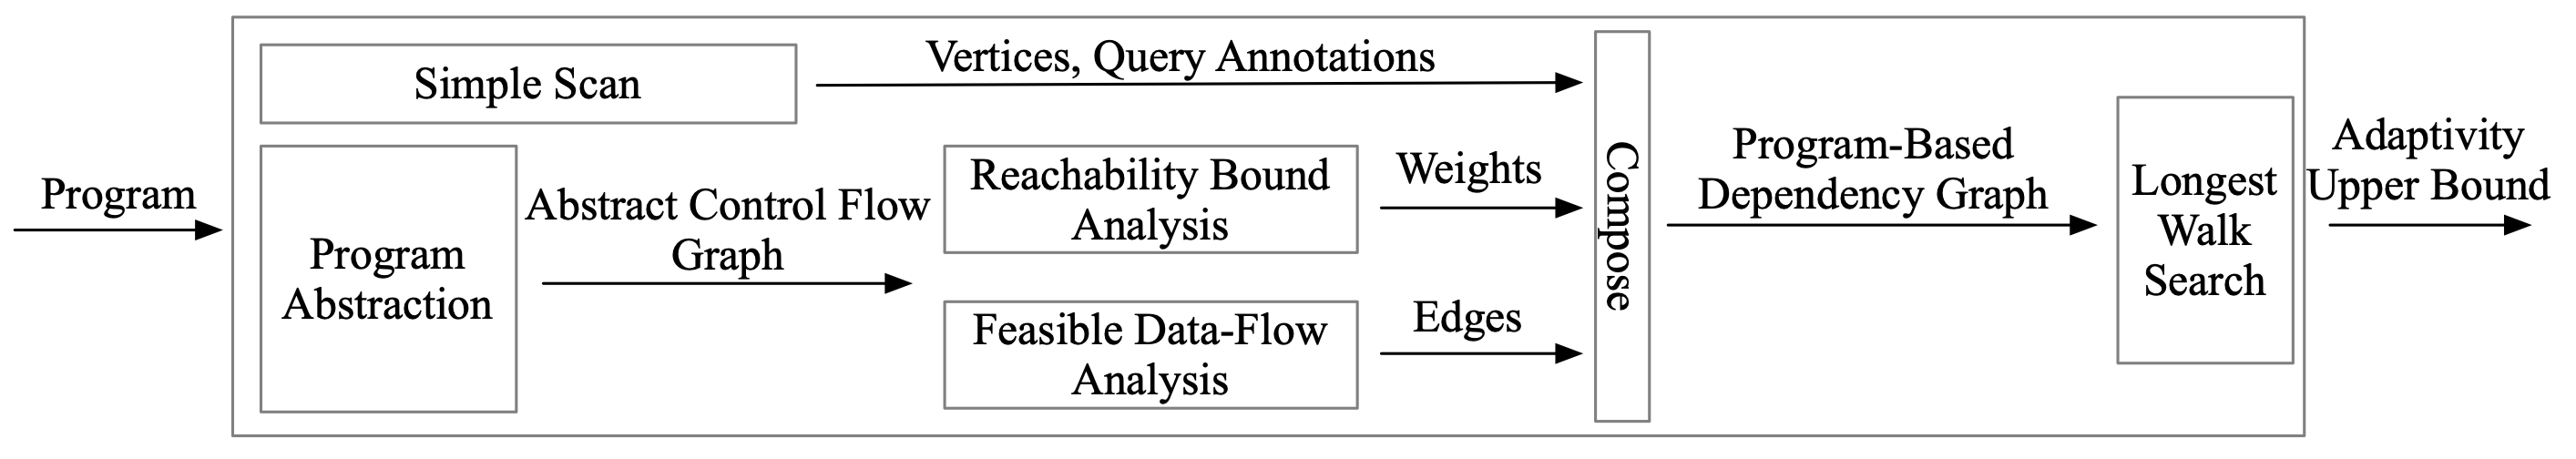
\includegraphics[width=1.0\columnwidth]{figures/adapfun.png}
      \vspace{-0.3cm}
      \caption{The overview of {\THESYSTEM}}
      \label{fig:adaptfun}
      \vspace{-0.5cm}
    \end{figure}
    
\subsubsection{Static Data Dependency Analysis}
\label{sec:static-datadep}
I develop a variant of data flow analysis, called Feasible Data-Flow Generation, which produces a sound approximation of the edges in the execution based dependency graph.
%  $\live_{in}(l,c)$ and $\live_{out}(l, c)$ is computed by the Standard worklist algorithm. (For simplicity, we use $\live(l,c)$ to represent $\live_{in}(l,c)$ in the other part of the paper.
%%
\paragraph{Feasible Data-Flow Generation}
We generate edges by using both control and data flow in the following $\flowsto$ relation, which uses the results of reaching definition analysis, as $\live(l, c)$ for every label $l$ in a program $c$. $\mathsf{FV}$ computes the set of free variables in an expression. 
% $\mathsf{blk}$ returns a list of labeled computation blocks of a labeled command $c$.
%
%   \[
%  \begin{array}{ll}
%     dcdg([x := e]^{l})  & = \{ (y^i, x^l) | y \in VAR(e) \land (y,i) \in \live_{in}(l) \}  \\
%      dcdg([x := q(e)]^{l})  & = \{ (y^i, x^l) | y \in VAR(e) \land (y,i) \in \live_{in}(l) \}  \\
%      dcdg([skip]^{l})  & = \emptyset \\
%      dcdg([if [b]^l then C_1 else C_2)  & =  dcdg(c_1) \cup dcdg(c_2)\\ & \cup \{(x^i,y^j) | x \in VAR(b) \land (x,i) \in \live_{in}(l) \land ([y = \_]^j) \in blocks(c_1) \} \\
%      &\cup \{(x^i,y^j) | x \in VAR(b) \land (x,i) \in \live_{in}(l) \land ([y = \_]^j) \in blocks(c_2) \} \\
%      dcdg([while [b]^l do c)  & =  dcdg(c) \cup \{(x^i,y^j) | x \in VAR(b) \land (x,i) \in \live_{in}(l) \land ([y = \_]^j) \in blocks(C) \} \\
%      dcdg(c_1 ;c_2)  & = dcdg(c_1) \cup  dcdg(c_2) \\
%  \end{array}
%  \]
%
\begin{defn}[Feasible Data-Flow]
  \label{def:feasible_flowsto}
  Given a program $c$ and two labeled variables $x^i, y^j$  in this program, 
  $\flowsto(x^i, y^j, c)$ is 
    {\footnotesize
    \[
   \begin{array}{ll}
    \flowsto(x^i, y^j, \clabel{\assign{x}{\expr}}{}^l)  & \triangleq (x^i, y^j) \in \{ (y^i, x^l) | y \in \mathsf{FV}(\expr) 
    % \land (y,i) \in \live(l, \clabel{\assign{x}{\expr}}^l) \}  \\
    \land y^i \in \live(l, \clabel{\assign{x}{\expr}}^l) \}  \\
    \flowsto(x^i, y^j, \clabel{\assign{x}{\query(\qexpr)}}{}^l)  & \triangleq (x^i, y^j) \in \{ (y^i, x^l) | y \in \mathsf{FV}(\qexpr) 
    % \land (y,i) \in \live(l,\clabel{\assign{x}{\query(\qexpr)}}^l) \}  \\
    \land y^i \in \live(l,\clabel{\assign{x}{\query(\qexpr)}}^l) \}  \\
    \flowsto(x^i, y^j, [\eskip]^{l})  & = \emptyset \\
    \flowsto(x^i, y^j, \eif ([b]^l, c_1, c_2))  & \triangleq \flowsto(x^i, y^j, c_1) \lor \flowsto(x^i, y^j, c_2) \\ 
        & \lor (x^i, y^j) \in
       \{(x^i,y^j) | x \in \mathsf{FV}(b) \land 
      %  (x,i) 
      x^i \in \live(l, \eif ([b]^l, c_1, c_2)) \land  y^j \in \lvar(c_1) \\
    %   ([y = \_]^j) \in \mathsf{blk}(c_1) \} \\
       &\lor (x^i, y^j) \in \{(x^i,y^j) | x \in \mathsf{FV}(b) \land 
      %  (x,i) 
      x^i\in \live(l, \eif ([b]^l, c_1, c_2))  \land  y^j \in \lvar(c_2) \\
    %   \land ([y = \_]^j) \in \mathsf{blk}(c_2) \} \\
       \flowsto(x^i, y^j, \ewhile [b]^l \edo c_w)  & \triangleq  \flowsto(x^i, y^j, c_w)  \lor
       \\ & 
       (x^i, y^j) \in  \{(x^i,y^j) | x \in \mathsf{FV}(b) \land 
      %  (x,i) 
      x^i \in \live(l,   \ewhile [b]^l \edo c_w) \land  y^j \in \lvar(c_w) \\
    %   ([y = \_]^j) \in \mathsf{blk}(c_w) \} \\
       \flowsto(x^i, y^j, c_1 ;c_2)  & \triangleq \flowsto(x^i, y^j, c_1) \lor \flowsto(x^i, y^j, c_2) \\
   \end{array}
   \]
   }
   \end{defn}
%
We prove that this \emph{Feasible Data-Flow} relation is a sound approximation 
of the \emph{variable may-Dependency} relation over labeled variables for every program,
in the appendix.
% ~\ref{apdx:flowsto_soundness}.
%
\paragraph*{Edge Estimation}
Then we define the estimated directed edges
% for each vertex in $\progV(c)$,
between vertices in $\progV(c)$,
as a set of pairs 
% $\progW(c) \in \mathcal{P}(\mathcal{LV} \times \mathcal{LV} \times EXPR(\constdom))$ 
$\progE(c) \in \mathcal{P}( \mathcal{LV} \times \mathcal{LV})$
% is the set of pairs 
% The weight for each vertex in $\progV(c)$ is computed 
indicating a directed edge from the first vertex to the second one in each pair
as follows,
{
  \[
    \begin{array}{ll}
    \progE(c) \triangleq &
    % \left
    \{ 
    (y^j, x^i) 
    % \in \mathcal{LV} \times \mathcal{LV}
    ~ \vert ~
    % \begin{array}{l}
      y^j, x^i \in \progV(c)
    \land
      % \\
      \exists n,
    %   \in \mathbb{N}, 
      z_1^{r_1}, \ldots, z_n^{r_n} \in \lvar(c) 
      \sthat 
    %   
    \\ 
    & \qquad \qquad
      n \geq 0 \land
    %   \\
      \flowsto(x^i,  z_1^{r_1}, c) 
      \land \cdots \land \flowsto(z_n^{r_n}, y^j, c) 
    % \end{array}
    % \right
    \}
    \end{array}
    \]
}
We prove that this estimated directed edge set $\progE(c)$ is a sound approximation of the 
edge set in $c$'s execution-based dependency graph 
in the appendix.
% ~\ref{apdx:adapt_soundness}.
%  \begin{defn}[Feasible Data-Flow]
%   \label{def:feasible_flowsto}
%     {\footnotesize
%     \[
%    \begin{array}{ll}
%       dcdg(\clabel{\assign{x}{\expr}}{}^l)  & = \{ (y^i, x^l) | y \in FV(e) \land (y,i) \in \live_{in}(l, \clabel{\assign{x}{\expr}}^l) \}  \\
%        dcdg(\clabel{\assign{x}{\query(\qexpr)}}{}^l)  & = \{ (y^i, x^l) | y \in FV(e) \land (y,i) \in \live_{in}(l,\clabel{\assign{x}{\query(\qexpr)}}^l) \}  \\
%        dcdg([\eskip]^{l})  & = \emptyset \\
%        dcdg([\eif [b]^l \ethen c_1 \eelse c_2)  & =  dcdg(c_1) \cup dcdg(c_2)\\ & \cup 
%        \{(x^i,y^j) | x \in FV(b) \land (x,i) \in \live_{in}(l) \land ([y = \_]^j) \in blocks(c_1) \} \\
%        &\cup \{(x^i,y^j) | x \in FV(b) \land (x,i) \in \live_{in}(l) \land ([y = \_]^j) \in blocks(c_2) \} \\
%        dcdg([\ewhile [b]^l \edo c)  & =  dcdg(c) \cup \{(x^i,y^j) | x \in FV(b) \land (x,i) \in \live_{in}(l) \land ([y = \_]^j) \in blocks(C) \} \\
%        dcdg(c_1 ;c_2)  & = dcdg(c_1) \cup  dcdg(c_2) \\
%    \end{array}
%    \]
%    }
%    \end{defn}
%    For any two labeled variables $x^i, y^j$ in a program $c$, 
%   %  it is easy to see that there is a one-on-one correspondence between 
%   %  $\flowsto$ relation of the two variables, and the $dcdg$ analysis result on $c$.
%   we use $\flowsto()$ denote if they have a feasible data-flow relation in Definition~\ref{def:flowsto}.
%    \begin{defn}[Feasible Data-Flow ($\flowsto$)]
%    \label{def:flowsto}
%    \[
%    \forall c \in \cdom, x^i, y^j \in \lvar_c \sthat 
%    \flowsto(x^i, y^j, c) \iff (x^i, y^j) \in dcdg(c)
%    \]
%    \end{defn}
  %  This soundness is proved in Proof~\ref{pf:rd_soundness} in appendix~\ref{apdx:rd_soundness}.
  %  For any two labeled variables in a program $c$, it is easy to see that there is a one-on-one correspondence between 
  %  $\flowsto$ relation of the two variables, and the $dcdg$ analysis result on $c$.
  %  \begin{thm}[Soundness of the Feasible Data-Flow Analysis]
  %  \label{thm:rd_soundness}
  %  \[
  %  \forall c \in \cdom, x^i, y^j \in \lvar_c \sthat 
  %  \flowsto(x^i, y^j, c) \iff (x^i, y^j) \in dcdg(c)
  %  \]
  %  \end{thm}
  %  This soundness is proved in Proof~\ref{pf:rd_soundness} in appendix~\ref{apdx:rd_soundness}.
  \paragraph*{Example}
 Look at Figure~\ref{fig:twoRounds_example}(c),
and take the edge $(l^6, a^5)$ for example.
By $\flowsto(l^6, a^5, c)$, we can see $a$ is used directly in the query expression $\chi[k]*a$,
in the assignment command $\clabel{\assign{l}{\query(\chi[k]*a)}}^l$,
i.e., $a \in FV(\chi[k]*a)$.
Also, from the reaching definition analysis, we know $a^5 \in \live(6, \kw{twoRounds(k)})$.
Then we have $\flowsto(l^6, a^5, c)$ and construct the edge $(l^6, a^5)$.
And the same way for constructing the rest edges. Also, the edge $(x^3,j^5)$ in the same graph represents the control flow, caught by our $\flowsto$ relation.
%
%   \subsection{Program-Based Data Dependency Graph Generation}
%   %  Weighted Data Dependency Graph Generation}
%   \label{sec:alg_graphgen}
   %
%    Each directed edge represents an abstract transition 
%    between two control locations, i.e., the labels of two commands (we call the labels also control location and they refer to the same thing in the follows), 
%    where the second labeled command will be executed after execution of the command with first label.
%    The abstract transition contains a set of difference constraints for variables, generated by abstracting the command of the first label.
%   \item Computing 
%   % we get the reachability bound for each command.
%   the symbolic reachability bound for each command,
%   % the value bound invariant for each variable in the event and 
%   by inferring the value bound invariant for each variable 
%   % the event transition closure over the abstract control flow graph,
%   and the transition closure for every abstract transition through the constraints over the abstract control flow graph.
%   % \\
%   % Through this graph and constraint for every transition, we infer the  invariant for every variable,
%   % and compute the transition closure for every abstract transition.
%   % By solving the closure with the invariants of variables involved in this closure for every transition, 
%   % we compute the symbolic reachability bound of every commands corresponding to 
% %     % this transition.
% %     \item Performing a feasible data-flow analysis from the reachable definition algorithm. 
% % %  By generating set of all the reachable variables at location of label $l$ in the program $c$.
% % and generating the set of all the reachable variables for every program location.
% % For every labelled variable $x^l$ in this set, 
% % the value assigned to that variable
% % in the assignment command associated to that label is reachable at the entry point of  executing the command of label $l$.
% % \item Refining the abstract control flow graph into a weighted-data dependency graph, 
% % by annotating each vertex with reachability bounds and 
% % removing unfeasible edges and redundant edges and vertices.
% % adding edges between
% %     variables having data-flow relations, and
% % removing the edges between locations where the variables associated to that labeled command isn't reachable from the second location.
% % \\
% % first annotate each vertex of label $l$ with the variable 
% % assigned in that labeled command, and remove the rest doesn't correspond to an assignment command.
% % Then 
% % add direct edge between two labeled variables,
% % where the first variable 
% % is directly used in the assignment expression to the second variable, by restricting 
% % the first labeled variable is reachable at the the second label.
% %
% \item Computing the adaptivity through this weighted data dependency graph,
%   by finding a finite walk on this weighted graph, 
% traversing the maximum times of query variables, by restricting the visiting time of every vertex on this walk to its weight.
% The maximum number of vertices corresponding to a query variables visited on this walk is the estimated upper bound, for program's adaptivity.

%    In this step, $\THESYSTEM$ refines the abstract control flow graph into the program-based weighted-data dependency graph, 
% by annotating each vertex with reachability bounds and 
% removing unfeasible edges and redundant edges and vertices,
% % This graph is used 
% for approximating the trace-based weight-data dependency graph.
% \\
% Specifically, we first annotate each vertex of label $l$ with the variable 
% assigned in that labeled command, and remove the rest doesn't correspond to an assignment command.
% Then 
% add direct edge between two labeled variables,
% where the first variable 
% is directly used in the assignment expression to the second variable, by restricting 
% the first labeled variable is reachable at the second label.
% % \\
% The formal definition is as follows.
% 

\subsubsection{Static Data Dependency Quantity Analysis}
\label{sec:static-quantity}

% In order to estimate weight for every vertex in the program-based dependency graph,
In order to estimate the \emph{Dependency-Quantity} from the execution-based analysis,
we perform the symbolic reachability bound analysis on the program's abstract control flow graph $\absG(c)$ firstly,
and add weight on that graph as shown in Figure~\ref{fig:abscfg_tworound}(c). 
% This because
% the vertices in the two graph share the same unique label, the line number.
% We would like to generate the closure of every edge, which is an equality relation between variables.  Solving this closure gives us the reachability bound for this edge. With all the bound for all the edges in the abstract control flow graph, we can calculate the weight for every vertex in this graph. For example, we show the closure generated for the edge $(4, j < j - 1, 5)$, 
% $\absclr(4, 5) = \varinvar(j)$. The invariant for variable $j$, $\varinvar(j)$ used here is 
% $\varinvar(j) = k * \absclr(1, 2)$, which is generated by all the difference constraints involving $j$ in the graph. Notice the $k$ in $\varinvar(j)$ comes from considering both difference constraint $j<=k$ from edge (1,2) and $j<=j-1$ from (4,5), which intuitively reflects the while loop whose counter is set to $k$ at the beginning and decreases by 1 at each iteration.
% We first generate the invariant for every variable showing up in the difference constraint and not user defined. For example, in the Figure~\ref{def:abscfg_tworound}(b), there are three variables $a$, $x$, $j$ that we will generate invariant for. We show the invariant for the counter $k$, which is $j = k$. 
% $\absclr(1, 2) = 1$
% \\
% => 
% $\absclr(4, 5) = k$
% using the difference constraint on the edges for all 
% through the edges in $\absG(c)$, which correspond to $c$'s abstract transition between labels.
% We infer the invariant for every variable, and compute the transition closure for every abstract transition. By solving the closure
% with the invariants of variables involved in this closure for every transition, we compute
% the symbolic reachability bound of every commands corresponding to this transition. Specifically, this analysis can be performed in four steps:
%  Variable Modification Tracking, Local Bounds Computation,
% Invariant Inference and Closure Generation, and Reachability Bound Computation,
% 
% We present the details of invariant, closure generation, and reachability bound computation as follows.
% with details as follows.
% \\
% %
% 1.  Variable Modification Tracking: collecting the dc for where each variable is increased, decreased and reset: 
% \\
% 2. Local Bounds Computation: 
% \\
% 3. Invariant Inference and Closure Generation
% \\
% 4. Reachability Bound Computation,
% %
% \paragraph*{Variable Modification Tracking}
% Identify the abstract events where each variable is increased, decreased and reset:
% \\
% $\inc: \mathcal{VAR} \to \mathcal{P}(\absevent) $
% the set of the abstract events where the variable increase.
% \\
% $\inc(x) = \{(\absevent, c) | \absevent = (l, l', x' \leq x + v)\}$
% \\
% $\reset: \mathcal{VAR} \to \mathcal{P}(\absevent) $
% The set of the abstract events where the variable is reset.
% \\
% $\dec: \mathcal{VAR} \to \mathcal{P}(\absevent) $
% The set of abstract events where the variable decrease.
% % \\
% % $\dec(x) = \{(\absevent, c) | \absevent = (l, l', x' \leq x - v)\}$
% \\
% $Incr(v) \triangleq \sum\limits_{(\absevent, c) \in \inc(v)}\{\absclr(\absevent) \times v\}$
% %
% \paragraph*{Local Bounds}
% Given a program $c$ with its abstract control flow graph 
% $\absG(c) = (\absV, \absE)$
% \\
% Local Bounds Computation:
% $\locbound: \absevent \to \mathcal{VAR} \cup \constdom$.
% %
% \[ 
% \begin{array}{ll}
%   \locbound(\absevent) \triangleq 1 
%   & \absevent \notin SCC(\absG(c))
%   \\
%   \locbound(\absevent) \triangleq (x, v) 
%   & \absevent \in SCC(\absG(c)) \land \absevent \in \dec(x) \land  \absevent = (\_, \_ , x' \leq x - v) \\
%   \locbound(\absevent) \triangleq (x, \max(\dec(x))) 
%   & \absevent \in SCC(\absG(c)) \land 
%   \absevent  \notin \bigcup_{x \in \mathcal{VAR}} \dec(x)
%   \land \absevent \notin SCC(\absG(c) \setminus \dec(x)) 
% \end{array}
%   \]
%   The first case is straightforward. Since variable's visiting time outside of any while loop is at most 1, we do not need to analyze the visiting times of every node in the graph from phase 1.
%   The second and third step is guaranteed by the \emph{Discussion on Soundness} in Section 4 of \cite{sinn2017complexity}.
%   Then soundness proof is in Lemma~\ref{lem:local_bound_sound} in appendix~\ref{apdx:reachability_soundness}.
% %
% \paragraph*{Invariant Inference and Closure Generation }
% Then, computing the bound invariants for variables and the transition closures for abstract events:
% \\ 
% $ \varinvar: \mathcal{VAR} \cup \constdom \to EXPR(\constdom)$
% \\
% $\absclr: \absevent \to EXPR(\constdom)$
% \\
% Then, the symbolic invariant for each variable 
% as well as the symbolic transition closure for each transition is calculated as follows:
% \[ 
% \begin{array}{lll}
%   \varinvar(x) & \triangleq c & c \in \constdom \\
%   \varinvar(x) & \triangleq Incr(v) + \max(\{\varinvar(a) + c | (t, a, c) \in \reset(x)\}) & c \notin \constdom
% \end{array}
% \]
% %
% \begin{defn}
%   \label{def:transition_closure_base}
% \[ 
% \begin{array}{lll}
%   \absclr(\absevent) 
%   & \triangleq x / v & \\ 
%   & \locbound(\absevent) = (x, v) \in \constdom \times \mathbb{N} & \\
%   \absclr(\absevent) 
%   & \triangleq (Incr(x) + 
%   \sum\limits_{(\absevent', y, v') \in \reset(x)}
%   \absclr(\absevent') \times \max(\varinvar(y) + v', 0) ) / v & \\
%   & \locbound(\absevent) = (x, v) \land x \notin \constdom & 
% \end{array}
%   \]
% \end{defn}
% %
% \paragraph*{Improved Variable Modification Tracking}
% Instead of just identifying the abstract events where each variable is reset,
% this improvement identifies the chain of the events where a given variable is reset by the 
% variables of the abstract events through the chain.
% \\
% $\resetchain: \mathcal{VAR} \to \mathcal{P}(\mathcal{P}(\absevent)) $
% The set of the chain of abstract events where the variable is reset through the chain.
% % \\
% % $Incr(v) \triangleq \sum\limits_{(\absevent, c) \in \inc(v)}\{\absclr(\absevent) \times v\}$
% %
% \paragraph*{Improved Invariant Inference and Closure Generation}
% Then, computing the bound invariants for variables and the transition closures for abstract events:
% \\ 
% $ \varinvar: \mathcal{VAR} \cup \constdom \to EXPR(\constdom)$
% \\
% $\absclr: \absevent \to EXPR(\constdom)$
% \\
% Then, the symbolic invariant for each variable 
% as well as the symbolic transition closure for each transition is calculated as follows:
% \[ 
% \begin{array}{lll}
%   \varinvar(x) & \triangleq c & c \in \constdom \\
%   \varinvar(x) & \triangleq Incr(v) + \max(\{\varinvar(a) + c | (t, a, c) \in \reset(x)\}) & c \notin \constdom
% \end{array}
% \]
% %
% \begin{defn}
%   \label{def:transition_closure}
% \[ 
% \begin{array}{lll}
%   \absclr(\absevent) 
%   & \triangleq x / v & \\ 
%   & \locbound(\absevent) = (x, v) \in \constdom \times \mathbb{N} & \\
%   \absclr(\absevent) 
%   & \triangleq \Big(
%     \sum\limits_{y \in \{ y ~|~ 
%     ch \in \resetchain(x), (l_1, x, y, v, l_2) \in ch \} } Incr(x) & \\
%     & \quad + 
%   \sum\limits_{ch \in \resetchain(x)}
%   \big( \min\limits_{\absevent' \in ch}({\absclr(\absevent')}) \times 
%   \max(\varinvar(y) + \sum\limits_{(l_1, x, y, v, l_2) \in ch } v, 0)\big) \Big) / v & \\
%   & \locbound(\absevent) = (x, v) \land x \notin \constdom & 
% \end{array}
%   \]
% \end{defn}
  %
% \paragraph*{Adding the Reachability Bounds for Every Vertex in the Data-Control Flow Graph}
% Updating the weight of every vertex in the $\progG(c) = (\progV, \progE, \progW, \progF)$ for program $c$ generated from phase 1. 
% For every $x^l \in \progV$, find the abstract event $\absevent \in \absflow(c)$ of the form $(l, \_, \_)$, updating the $\progW(x^l) $ by the transition closure of this event.
% \\
% \paragraph*{Reachability Bound Computation}
% With all the closures for all the edges of the abstract control flow graph, we can solve them to obtains the reachability bound of every edges. We decide the weight for every vertex in the abstract control flow graph by using the bound of the edges which head out from this vertex, by taking the max of the bound from these involving edges. For instance,   
% By the constraint on the edge $(4, j \leq j - 1, 5)$, we get bound $k$ for this edge.
% Then, we assign vertex $4$ by reachability bound $k$, as in Figure~\ref{fig:abscfg_tworound}(c). 
% Another interesting vertex is $2$, which has more than one edge heading out from it, $(2, \top, 3)$ and $(2,\top, 6)$. For the weight for vertex $2$, we choose the max between the bound $k$ from $(2,\top, 3)$ and $1$ from $(2,\top, 6)$.
% we first infer its local bound as variable $j$.
% Then by solving the invariant for variable $j$,
% we infer the value bound for $j$, which is $k$.
% Then the reachability bound for this abstract transition, (i.e., edge $4, j \leq j - 1, 5$) 
% is computed as $k$ as well through Definition~\ref{def:abs_trace}.
% \\
% $
% \progW(x^l) 
%   \triangleq \absclr(\absevent)
% $
% Through the transition closure computed above, 
% The weight of every label in 
% % Then we update 
% the program $c$'s abstract control flow graph,
% $\absG(c) =(\absV, \absE, \absW)$
% is 
% computed as the maximum over all the abstract events $\absevent \in \absE$ heading out from this vertex, formally as follows.
% % by annotating each vertex with a symbolic weight. 
% % This weight corresponds to 
% %reachability bounds of
% \\
% $\absW 
% \triangleq \left\{ (l, w) \in \mathbb{N} \times EXPR(\constdom) | w = \max\limits_{\absevent = (l, \_, \_)} \{ \absclr(\absevent)\} \right\}$.
% % \\
% \paragraph*{Example}
% Still looking at the two-round example as in Figure~\ref{fig:abscfg_tworound}(b) where 
% each label $l$ is added with a weight by $absW$.
% This weight represents the  maximum reaching times of this location $l$, in the other word,
% the estimated maximum visiting times of the command labeled with $l$.
% For example, looking at the vertex $1$,
% by analysis steps, since it isn't in any SCC, it's estimated reachability bound is computed as $1$.
% However, for the vertex $4$ which is involved in an SCC, the reachability bound is inferred in another way.
% By the constraint on the edge $4, j \leq j - 1, 5$,
% we first infer its local bound as variable $j$.
% Then by solving the invariant for variable $j$,
% we infer the value bound for $j$, which is $k$.
% Then the reachability bound for this abstract transition, (i.e., edge $4, j \leq j - 1, 5$) 
% is computed as $k$ as well through Definition~\ref{def:abs_trace}.
% In this abstract control flow graph, every vertex is a label,
% corresponding to a label command in the program.
% Each directed 
% edge represents an abstract transition 
% between two control locations, 
% i.e., the labels of two commands (we call the labels also control location and they refer to the same thing), 
% where the second labeled command will be executed after execution of the command with first label.
% For example, the edge $0, a \leq 0, 1$ on the top, represents,
% from location $0$, the command 
% $\clabel{\assign{a}{0}}^0$ is executed with next continuation location $1$,
% where the 
% command $\clabel{\assign{j}{k}}^1$ will be executed next.
% The constraint $a \leq 0$ is generated by abstracting from the assignment command $\assign{a}{0}$,
% representing that value of $a$ is less than or equals to $0$ after 
% location $0$ before executing command at line $1$.
%
% The same way for the rest weights' computation.
% We use for 
The computed weights $\absW(c)$ is
a set of pairs 
$(l, w)$ where 
$w$ is the weight 
for label $l$ from the abstract control flow graph of $c$.
% The weight $w$ for each label $l$ 
$w$ is an arithmetic  expression over $\mathbb{N}$ and
input variables, denoted by $\mathcal{A}_{in}$.
This analysis is  inspired from the program complexity analysis method in \cite{sinn2017complexity}.
The detail of our symbolic reachability bound analysis which uses the difference constraint of the abstract control flow graph can be found in the appendix.
%
%
\paragraph{Reachability Bound Estimation}
% The weight for each vertex in $\progV(c)$ is computed as follows,
With the computed weights $\absW(c)$ for program $c$,
we compute the reachability bound for each labeled variable $x^l$ as the estimation of the 
execution-based \emph{Dependency-Quantity}. 
% vertex in $\progV(c)$,
% as a set of pairs $(x^l, w) \in \ldom \times \mathcal{A}_{in}$
% $\progW(c) \in \mathcal{P}(\mathcal{LV} \times \mathcal{LV} \times EXPR(\constdom))$ 
% is the set of pairs 
% The weight for each vertex in $\progV(c)$ is computed 
The estimated the reachability bound mapping each $x^l \in \lvar(c)$ to an arithmetic  expression over $\mathbb{N}$ and
input variables. 
\[ 
  rb_{\kw{prog}}(x^l) = w \st (l, w) \in \absW(c)
  \]
% Because
% the vertices in the two graph share the same unique label, the line number of the same command,
% we define 
%
We prove that this 
% symbolic expression is the upper bound for $x^l$'s 
arithmetic expression for $x^l \in \progV(c)$ is a sound upper bound of 
the maximum visiting times of $x^l$ over all execution traces of $c$, with the full proof in the appendix.
  \begin{thm}[Soundness of the Reachability Bounds Estimation]
    \label{thm:addweight_soundness}
  Given a program ${c}$ with its estimated weight $\progW(c)$
%   program-based dependency graph 
%   $\progG = (\progV, \progE, \progW, \progF)$,
  % $\traceG = (\traceV, \traceE, \traceW, \traceF)$, 
  we have:
    %
  \[
  \forall x^l \in \lvar(c), \vtrace_0 \in \mathcal{T}_0(c), \trace \in \mathcal{T},
  v \in \mathbb{N}
   \st 
  % \max \left\{ 
    % \vcounter(\vtrace') l ~ \middle\vert~
  % \forall \vtrace, \trace' \in \mathcal{T} \st 
  % \config{{c}, \trace_0} \to^{*} \config{\eskip, \trace_0 \tracecat\vtrace} 
  % \land 
  \config{\vtrace_0, w} \earrow v
  \implies
  % \right\} 
  rb(x^l) \trace_0 \leq v
  \]
  \end{thm}
% appendix~\ref{apdx:reachability_soundness}. 
%
Based on $\rb_{\kw{prog}}$, we construct a set of weights as follows. 
This set of weights is used to in estimating the dependency graph in step3.
$\progW(c)$ is defined
% denoted by $\mathcal{A}_{in}$
as follows,
% :
% \\
 \[\progW(c) \triangleq
  \left
  \{ (x^l,  rb_{\kw{prog}}(x^l)) \mid x^l \in \lvar(c) 
\right \}.
\]
\paragraph*{Example} 
As in
Figure~\ref{fig:twoRounds_example}(c),
the weight for $a^5$ is $k$. which is a sound estimated weight.
% in program-based dependency Graph as $k$ as well.
For any initial $\trace_0 \in \mathcal{T}_0(c)$, we know $\config{\trace_0, k} \earrow \env(\trace_0) k$ and
the weight $w_k$ for vertex $a^5$ from Figrue~\ref{fig:twoRounds_example}(b)
$w_k(\trace_0) = \env(\trace_0) k$. 
%
In the same way, the weights for all the other vertices are sound.
% for the rest weights' computation.

\subsubsection{Adaptivity Estimation}
\label{sec:static-adapt}
% \subsection{Program-Based Data Dependency Graph Generation}
% %  Weighted Data Dependency Graph Generation}
%  \label{sec:alg_graphgen}
 %
%    Each directed edge represents an abstract transition 
%    between two control locations, i.e., the labels of two commands (we call the labels also control location and they refer to the same thing in the follows), 
%    where the second labeled command will be executed after execution of the command with first label.
%    The abstract transition contains a set of difference constraints for variables, generated by abstracting the command of the first label.
%   \item Computing 
%   % I get the reachability bound for each command.
%   the symbolic reachability bound for each command,
%   % the value bound invariant for each variable in the event and 
%   by inferring the value bound invariant for each variable 
%   % the event transition closure over the abstract control flow graph,
%   and the transition closure for every abstract transition through the constraints over the abstract control flow graph.
%   % \\
%   % Through this graph and constraint for every transition, I infer the  invariant for every variable,
%   % and compute the transition closure for every abstract transition.
%   % By solving the closure with the invariants of variables involved in this closure for every transition, 
%   % I compute the symbolic reachability bound of every commands corresponding to 
% %     % this transition.
% %     \item Performing a feasible data-flow analysis from the reachable definition algorithm. 
% % %  By generating set of all the reachable variables at location of label $l$ in the program $c$.
% % and generating the set of all the reachable variables for every program location.
% % For every labelled variable $x^l$ in this set, 
% % the value assigned to that variable
% % in the assignment command associated to that label is reachable at the entry point of  executing the command of label $l$.
% % \item Refining the abstract control flow graph into a weighted-data dependency graph, 
% % by annotating each vertex with reachability bounds and 
% % removing unfeasible edges and redundant edges and vertices.
% % adding edges between
% %     variables having data-flow relations, and
% % removing the edges between locations where the variables associated to that labeled command isn't reachable from the second location.
% % \\
% % first annotate each vertex of label $l$ with the variable 
% % assigned in that labeled command, and remove the rest doesn't correspond to an assignment command.
% % Then 
% % add direct edge between two labeled variables,
% % where the first variable 
% % is directly used in the assignment expression to the second variable, by restricting 
% % the first labeled variable is reachable at the the second label.
% %
% \item Computing the adaptivity through this weighted data dependency graph,
%   by finding a finite walk on this weighted graph, 
% traversing the maximum times of query variables, by restricting the visiting time of every vertex on this walk to its weight.
% The maximum number of vertices corresponding to a query variables visited on this walk is the estimated upper bound, for program's adaptivity.

%    In this step, $\THESYSTEM$ refines the abstract control flow graph into the program-based weighted-data dependency graph, 
% by annotating each vertex with reachability bounds and 
% removing unfeasible edges and redundant edges and vertices,
% % This graph is used 
% for approximating the trace-based weight-data dependency graph.
% \\
% Specifically, I first annotate each vertex of label $l$ with the variable 
% assigned in that labeled command, and remove the rest doesn't correspond to an assignment command.
% Then 
% add direct edge between two labeled variables,
% where the first variable 
% is directly used in the assignment expression to the second variable, by restricting 
% the first labeled variable is reachable at the second label.
% % \\
% The formal definition is as follows.
Based on the variable \emph{may-dependency} relation in Section~\ref{sec:dynamic-datadep} and 
the dependency quantity analysis in Section~\ref{sec:dynamic-reachability}.
% gives us the edges, 
I firstly define the execution-based dependency graph, then formalize the \emph{adaptivity} in this section.

\subsubsection{Program-Based Data Dependency Graph Generation}
%  Weighted Data Dependency Graph Generation}
 \label{sec:alg_graphgen}
\todo{Remove:
 To build the graph, we firstly estimate the vertices and query annotations straightforwardly as follows.
\paragraph{Vertices Estimation and Query Annotation Estimation}
\label{sec:alg_vertexgen}
The vertices in the static analysis dependency graph are actually identical as the  Execution-Based Dependency Graph, which are assigned variables in the program annotated with the unique label(line number). These vertices are collected by statically scanning the program, like what I do for vertices of its Execution-Based Dependency Graph. The vertices are defined formally as follows.
%
  \highlight{
\[
    \progV(c) \triangleq \left\{ 
  x^l \in \mathcal{LV} 
  ~ \middle\vert ~
  x^l \in \lvar_{c}
  \right\}
  \]
  }
  %
%
The static scanning of the programs also tells us whether one vertice(assigned variable) is assigned by a query request.  I have similar definition when defining the Execution-Based Dependency Graph, 
a set of pairs $\progF(c) \in \mathcal{P}(\mathcal{LV} \times \{0, 1\} )$ 
% is the set of pairs 
% The weight for each vertex in $\progV(c)$ is computed 
mapping each $x^l \in \progV(c)$ to a flag, either $0$ or $1$, where $1$  means $x^{l}$ is a member of $ \qvar_{c}$, a set of those variables assigned with query requests,
and $0$ means $x^{l}$ not in this set. It is defined formally below.
\[\progF(c) =\left\{(x^l, n)  \in  \mathcal{LV} \times \{0, 1\} 
~ \middle\vert ~
x^l \in \lvar_{c},
n = 1 \iff x^l \in \qvar_{c} \land n = 0 \iff  x^l \not\in \qvar_{c} .
\right\}\]
Then, I build the estimated data dependency graph based on the above program static analysis as follows:
\\
\highlight{
\[
  \progG(c) = (\progV(c), \progE(c), \progW(c), \progF(c))
  \]
}
with $\progV(c), \progE(c), \progW(c)$ and $ \progF(c)$ as computed in each steps above.
% and $\progF(c) =\left\{(x^l, n)  \in  \mathcal{LV} \times \{0, 1\} 
% ~ \middle\vert ~
% x^l \in \lvar_{c},
% n = 1 \iff x^l \in \qvar_{c} \land n = 0 \iff  x^l \in \qvar_{c} .
% \right\} $,
This program-based graph program-based graph has a similar topology structure as 
% the one
% of 
the Execution-Based Dependency Graph. It has the same
vertices and query annotations, but approximated edges and weights.  
% The algorithm computation is 
It is formally defined in Definition~\ref{def:prog_graph}.
% Through the reachable definition set on every label,
% I remove the edges between labels where the variables associated to that labeled command isn't reachable from the second location.
%\absG(c) =(\absV, \absE, \absW)
\begin{defn}
[Program-Based Dependency Graph]
\label{def:prog_graph}
% [Program-Based Weighted Data Dependency Graph Generation Algorithm]
% \label{def:analyz_dcfg}
Given a program $c$, with its abstract weighted control flow graph $\absG(c) = (\absV, \absE, \absW)$ and 
feasible data flow relation $\flowsto(x^i, y^j, c)$ for every $x^i, y^j \in \lvar_c$, its Program-Based Weighted Data Dependency Graph
$\progG(c) = (\progV, \progE, \progW, \progF)$,
is generated as follows,
% \\
% \highlight{
% $\progV =\{x^l | x^l \in \lvar_c\} $
% \\
% $\progE = \{(y^i, x^l) | (y^i, x^l)  \in dcdg(c) \}$
% \\
% $\progW = \{(x^l, w ) | (l, w ) \in \absW \land x^l \in \lvar_c\}$
% \\
% $\progF = \{(l, q) \in \mathcal{L} \times \{0, 1\}| q = 1 \iff l \in \qvar_c, q = 0 \iff l \notin \qvar_c \}$.
% }
% \end{defn}
% \begin{defn}
% [Program-Based Dependency Graph].
% \label{def:prog_graph}
%   % \\
% Given a program ${c}$
% its program-based graph 
% $\progG({c}) = (\vertxs, \edges, \weights, \qflag)$ is defined as:
{\footnotesize
\[
\begin{array}{rlcl}
\text{Vertices} &
\progV & := & \left\{ 
x^l \in \mathcal{LV} 
~ \middle\vert ~
x^l \in \lvar_{c}
\right\}
\\
\text{Directed Edges} &
\progE & := & 
\left\{ 
({x}_1^{i}, {x}_2^{j}) \in \mathcal{LV} \times \mathcal{LV}
~ \middle\vert ~
\begin{array}{l}
{x}_1^{i}, {x}_2^{j} \in \vertxs
\land
% \\
\exists n \in \mathbb{N}, z_1^{r_1}, \cdots, z_n^{r_n} \in \lvar_{{c}} \sthat  
n \geq 0 \land
\\
\flowsto(x^i,  z_1^{r_1}, c) 
\land \cdots \land \flowsto(z_n^{r_n}, y^j, c) 
\end{array}
\right\}
\\
\text{Weights} &
\progW & := &
% \bigcup
% \begin{array}{l}
\left\{ (x^l, w) \in  \mathcal{LV} \times \mathcal{A}_{in}
\mid
x^l \in \lvar_{{c}} \land (l, w) \in \absW(c)
\right\}
% \end{array} 
\\
\text{Query Annotation} &
\progF & := & 
\left\{(x^l, n)  \in  \mathcal{LV} \times \{0, 1\} 
~ \middle\vert ~
x^l \in \lvar_{c},
n = 1 \iff x^l \in \qvar_{c} \land n = 0 \iff  x^l \in \qvar_{c} .
\right\}
\end{array}
\] }
\end{defn}
}
Finally we build the estimated data dependency graph based on the above program static analysis as follows:
\\
\highlight{
  \[
    % \progG(c) = (\progV(c), \progE(c), \progW(c), \progF(c))
    \progG(c) = (\progV(c), \progE(c))
    \]
}
with $\progV(c)$ and  $\progE(c)$
as computed in each steps above.
%
This program-based graph program-based graph has a similar topology structure as 
% the one
% of 
the Execution-Based Dependency Graph. It has the same
vertices 
% and query annotations, 
but approximated edges and weights.  
% The algorithm computation is 
It is formally defined in Definition~\ref{def:prog_graph}.
% Through the reachable definition set on every label,
% we remove the edges between labels where the variables associated to that labeled command isn't reachable from the second location.
%\absG(c) =(\absV, \absE, \absW)
\begin{defn}
  [Program-Based Dependency Graph]
  \label{def:prog_graph}
  % [Program-Based Weighted Data Dependency Graph Generation Algorithm]
% \label{def:analyz_dcfg}
Given a program $c$, with its abstract weighted control flow graph $\absG(c) = (\absV, \absE, \absW)$ and 
feasible data flow relation $\flowsto(x^i, y^j, c)$ for every $x^i, y^j \in \lvar_c$, its Program-Based Weighted Data Dependency Graph
$\progG(c) = (\progV, \progE)$,
is generated as follows,
% \\
% \highlight{
% $\progV =\{x^l | x^l \in \lvar_c\} $
% \\
% $\progE = \{(y^i, x^l) | (y^i, x^l)  \in dcdg(c) \}$
% \\
% $\progW = \{(x^l, w ) | (l, w ) \in \absW \land x^l \in \lvar_c\}$
% \\
% $\progF = \{(l, q) \in \mathcal{L} \times \{0, 1\}| q = 1 \iff l \in \qvar_c, q = 0 \iff l \notin \qvar_c \}$.
% }
% \end{defn}
% \begin{defn}
  % [Program-Based Dependency Graph].
  % \label{def:prog_graph}
%   % \\
% Given a program ${c}$
% its program-based graph 
% $\progG({c}) = (\vertxs, \edges, \weights, \qflag)$ is defined as:
{\footnotesize
\[
\begin{array}{lcl}
% \text{Vertices} &
% \progV & := & \left\{ 
% x^l \in \mathcal{LV} 
% ~ \middle\vert ~
% x^l \in \lvar_{c}
% \right\}
% \\
% \text{Directed Edges} &
% \progE & := & 
% \left\{ 
% ({x}_1^{i}, {x}_2^{j}) \in \mathcal{LV} \times \mathcal{LV}
% ~ \middle\vert ~
% \begin{array}{l}
%   {x}_1^{i}, {x}_2^{j} \in \vertxs
% \land
%   % \\
%   \exists n \in \mathbb{N}, z_1^{r_1}, \cdots, z_n^{r_n} \in \lvar_{{c}} \st 
%   n \geq 0 \land
%   \\
%   \flowsto(x^i,  z_1^{r_1}, c) 
%   \land \cdots \land \flowsto(z_n^{r_n}, y^j, c) 
% \end{array}
% \right\}
% \\
\progV(c) & \triangleq &
% \bigcup
% \begin{array}{l}
\left\{ (x^l, w) \in  \mathcal{LV} \times \mathcal{A}_{in}
\mid
x^l \in \lvar_{{c}} \land (l, w) \in \absW(c)
\right\}
\\
\progE(c) & \triangleq &
   \Big\{ (x^i, w, y^j) \in \mathcal{LV} \times 
   \mathcal{A}_{\kw{in}} \times \mathcal{LV}
~\mid~
  \\ & & \quad 
x^i, y^j \in \lvar(c) \land \flowsto(x^i, y^j, c) \land
  \exists n \in \mathbb{N}, z_1^{r_1}, \cdots, z_n^{r_n} \in \lvar_{{c}} \sthat 
  n \geq 0 
  % \\ & & \quad 
  % \flowsto(x^i,  z_1^{r_1}, c) 
  \land \cdots \land \flowsto(z_n^{r_n}, y^j, c) 
  \\ & & \quad 
  \land
  w = \max \left\{ \absclr(\absevent) ~\mid~ \absevent \in \absflow(c) \land \absevent = (i, \_, j) \right\} 
\Big\}.
\end{array}
\] }
\end{defn}

\highlight{
Comparing to previous works, this program-based graph program-based graph has a similar topology structure as 
% the one
% of 
the Execution-Based Dependency Graph. It has the same
vertices and query annotations, but approximated edges and weights.  
Benefited from the same topology structure and the extra quantity analysis, this new approximated dependency capture
the dependency and quantity information more precise than the previous
estimated dependency graph.
In this sense, it helps in estimating a tighter bound on the adaptivity than before.
}
\todo{Remove: 
Then, the Following part computes the adaptivity upper bound for a program $c$.
% Given a program ${c}$, we generate
\\
With
% its 
$c$'s program-based data dependency graph $\progG({c})$ approximated above,
%
its adaptivity upper bound 
% Defined in Definition~\ref{def:prog_adapt} as 
%
is estimated as
the maximum query length over all finite walks in $\walks(\progG({c}))$ formally in Definition~\ref{def:prog_adapt}, 
and computed 
% is computed as the maximum query length over all finite walks in $\walks(\progG({c}))$, and computed 
in Algorithm~\ref{alg:adpt_alg}.
% We use $\walks(\progG(c))$ represents the walks over the program-based dependency graph for $c$.
Different from the finite walk on a program $c$'s execution based graph,
%  $\traceG(c)$, 
% $k \in \walks(\progG(c))$ 
the finite walk in $\progG(c)$ doesn't rely on initial trace.
The occurrence times of every $v_i $ in $k$'s vertex sequence is bound by 
an arithmetic expression $w_i$ where $(v_i, w_i) \in \progW(c)$, is $v_i$'s estimated weight. 
% Then $\qlen(k) \in \mathcal{A}_{in}$ as well. 
% The full definition for $\walks(\progG(c))$ and $\qlen$ over $\walks(\progG(c))$ is in Apdix.
%
Formally defined as follows.
\begin{defn}[Finite Walk on Program-Based Dependency Graph ($k$)]
\label{def:prog_finitewalk}
Given a program $c$'s program-based dependency graph 
$\progG({c}) = (\progV(c), \progE(c), \progW(c), \progF(c))$, 
a \emph{finite walk} $k$ in $\traceG({c})$ is
% function $k: \mathcal{T} \to $ 
% sequence of edges.
% For a initial trace $\trace_0 \in \mathcal{T}$, 
% $k(\trace_0)$ is
a sequence of edges $(e_1 \ldots e_{n - 1})$ 
for which there is a sequence of vertices 
$(v_1, \ldots, v_{n})$ such that:
\begin{itemize}
    \item $e_i = (v_{i},v_{i + 1}) \in \progE(c)$ for every $1 \leq i < n$.
    \item every vertex $v_i \in \progV(c)$,
    and $(v_i, w_i) \in \progW(c)$, 
      $v_i$ appears in $(v_1, \ldots, v_{n})$ at most 
  $w_i$
    times.  
\end{itemize}
%
The length of $k$ is the number of vertices in its vertex sequence, i.e., $\len(k) = a$.
\end{defn}
We abuse the notation $\walks(\progG(c))$ represents the walks over the program-based dependency graph for $c$.
Different from the walks on a program $c$'s execution based graph,
$k \in \walks(\traceG(c))$, 
$k \in \walks(\progG(c))$ doesn't rely on initial trace.
The occurrence times of every $v_i $ in $k$'s vertex sequence is bound by 
an arithmetic expression $w_i$ where $(v_i, w_i) \in \progW(c)$, is $v_i$'s estimated weight. 
% Notice here, for a walk in $\progG(c)$, the occurrence times of every vertex in vertices sequence, 
%  and its 
The length of a finite walk $k \in \walks(\progG(c))$ is an arithmetic expression
as well, i.e., $\len(k) \in \mathcal{A}_{in}$
\\
Then the query length of a finite walk in  $\progG(c)$ is an arithmetic expression as well as follows,
%  $\qlen(k) \in \mathcal{A}_{in}$ as well. 
% The adaptivity upper bound 
% is estimated as
% Then the adaptivity bound based on program analysis for ${c}$ 
% is the number of query vertices on a finite walk in $\progG({c})$. This finite walk satisfies:
% \begin{itemize}
% \item the number of query vertices on this walk is maximum
% \item the visiting times of each vertex $v$ on this walk is bound by its reachability bound $\weights(v)$.
% \end{itemize}
\begin{defn}[Query Length of the Finite Walk on Program-Based Dependency Graph ($\qlen$)]
\label{def:static-qlen}
Given 
% labelled weighted graph $G = (\vertxs, \edges, \weights, \qflag)$, 
a program $c$'s execution-based dependency graph 
$\progG({c}) = (\progV(c), \progE(c), \progW(c), \progF(c))$, 
  and a \emph{finite walk} $k \in \walks(\progG(c))$,
The query length of $k$, $\qlen(k) \in \mathcal{A}_{in}$ 
% is a function $\qlen(k): \mathcal{T} \to \mathbb{N}$, such that with an initial trace  $\trace_0 \in \mathcal{T}$, 
% $\qlen(k)(\trace_0)$ 
is the number of vertices which correspond to query variables in the vertices sequence of this walk $k$
$(v_1, \ldots, v_{n})$ as follows, 
\[
  \qlen(k) = |\big( v \mid v \in (v_1, \ldots, v_{n}) \land \qflag(v) = 1 \big)|.
\]
% , where $\trace_0 \in \mathcal{T}$ is the initial trace and $\big(v \mid v \in (v_1, \ldots, v_{n}) \land \qflag(v) = 1 \big)$ is a subsequence of $(v_1, \ldots, v_{n})$.
%  $k$'s vertex sequence.
% \mg{If I understand where you want to go, why don't you just use the cardinality of the set above, rather than taking the length of a subsequence?}
% \jl{because the same vertex could have multiple occurrence in the sequence, and we will count all the occurrence instead of just once.
% So the cardinality of set doesn't work.}
\end{defn}
% is computed as the maximum query length over all finite walks in $\walks(\progG({c}))$, and computed 
% It is formally defined in \ref{def:prog_adapt}.
% defined formally as follows.
%
%
\begin{defn}
[{Program-Based Adaptivity}].
\label{def:prog_adapt}
\\
{
Given a program ${c}$ and its program-based graph 
$\progG({c})$
%  = (\vertxs, \edges, \weights, \qflag)$,
%
the program-based adaptivity for $c$ is 
% a function $\progA({c}): \mathcal{T} \to\mathbb{N} $,
% for an initial trace $\trace_0 \in \mathcal{T}$,
defined as%
\[
\progA({c})
\triangleq \max
\left\{ \qlen(k) \ \mid \  k \in \walks(\progG(c))\right \}.
\]
}
\end{defn}
Based on our soundness of the program-based adaptivity, our program-based adaptivity is a sound upper bound of its adaptivity in Definition~\ref{def:trace_adapt}. 
\begin{thm}[Soundness of \THESYSTEM]
  \label{thm:sound_progadapt}
  For every program $c$, 
  % for any initial trace $\trace_0$, 
  its program-based adaptivity is a sound upper bound of its adaptivity.
    $$  \progA(c) \geq A(c)$$
\end{thm}
For $\progA(c) \geq A(c)$ comparing between function and arithmetic expression,
we are specifically comparing, $\forall \trace \in \mathcal{T} \sthat  
\config{A(c), \trace} \earrow n \implies n \geq A(c)(\trace) $.
To estimate a sound and precise upper bound on adaptivity, we develop an adaptivity estimation algorithm called $\pathsearch$ (in Apdix Algorithm~I), which uses both the deep first search and breath first search strategy to find the walk. We also show that the estimated adaptivity from our $\pathsearch$ is sound with respect to the program-based adaptivity. 
\begin{thm}[Soundness of $\pathsearch$]
  \label{thm:sound_adaptalg}
  For every program $c$.
  % for any initial trace $\trace_0$,
    $$\pathsearch(\progG({c})) \geq \progA(c).$$
\end{thm}
}
\subsubsection{Adaptivity Estimation}
%  Weighted Data Dependency Graph Generation}
\label{sec:static-adapt-comput}
% \subsubsection{Adaptivity Upper Bound Computation}
%  from refined weighted-labeled data-flow graph}
This phase computes the adaptivity upper bound for a program $c$.
% Given a program ${c}$, we generate
\\
With
% its 
$c$'s program-based data dependency graph $\progG({c})$ approximated above,
%
its adaptivity upper bound 
% Defined in Definition~\ref{def:prog_adapt} as 
%
is estimated as
% Then the adaptivity bound based on program analysis for ${c}$ 
% is the number of query vertices on a finite walk in $\progG({c})$. This finite walk satisfies:
% \begin{itemize}
% \item the number of query vertices on this walk is maximum
% \item the visiting times of each vertex $v$ on this walk is bound by its reachability bound $\weights(v)$.
% \end{itemize}
the maximum query length over all finite walks in $\walks(\progG({c}))$ formally in Definition~\ref{def:prog_adapt}, 
and computed 
% is computed as the maximum query length over all finite walks in $\walks(\progG({c}))$, and computed 
in Algorithm~\ref{alg:adpt_alg}.
%
% It is formally defined in \ref{def:prog_adapt}.
% defined formally as follows.
%
% %
% \begin{defn}
% [{Program-Based Adaptivity}].
% \label{def:prog_adapt}
% \\
% {
% Given a program ${c}$ and its program-based graph 
% $\progG({c})$
% %  = (\vertxs, \edges, \weights, \qflag)$,
% %
% the program-based adaptivity for $c$ is defined as%
% \[
% \progA({c}) 
% \triangleq \max
% \left\{ \qlen(k)\ \mid \  k\in \walks(\progG({c}))\right \}.
% \]
% }
% \end{defn} 

% We use $\walks(\progG(c))$ represents the walks over the program-based dependency graph for $c$.
Different from the finite walk on a program $c$'s execution based graph,
%  $\traceG(c)$, 
% $k \in \walks(\progG(c))$ 
the finite walk in $\progG(c)$ doesn't rely on initial trace.
The occurrence times of every $v_i $ in $k$'s vertex sequence is bound by 
an arithmetic expression $w_i$ where $(v_i, w_i) \in \progV(c)$, is $v_i$'s estimated weight. 
% Then $\qlen(k) \in \mathcal{A}_{in}$ as well. 
% The full definition for $\walks(\progG(c))$ and $\qlen$ over $\walks(\progG(c))$ is in Apdix.
%
Formally defined as follows.
\begin{defn}[Finite Walk on Program-Based Dependency Graph ($k$)].
  \label{def:prog_finitewalk}
  \\
%   Given a program $c$'s execution-based dependency graph $\traceG({c})(\trace)$, 
%   a \emph{finite walk} $fw$ in $\traceG({c})(\trace)$ is a sequence of edges $(e_1 \ldots e_{n - 1})$ 
%   for which there is a sequence of vertices $(v_1, \ldots, v_{n})$ such that:
%   \begin{itemize}
%       \item $e_i = (v_{i},v_{i + 1})$ for every $1 \leq i < n$.
%       \item every vertex $v \in \traceV({c}) $ appears in $(v_1, \ldots, v_{n})$ at most 
%       \wq{$\traceW({c})(\trace)$} times.  
%   \end{itemize}
%   %
%   The length of $fw$ is the number of vertices in its vertex sequence, i.e., $\len(k) = n$.
  Given a program $c$'s program-based dependency graph 
  $\progG({c}) = (\progV(c), \progE(c))$
  % , \progW(c), \progF(c))$, 
  a \emph{finite walk} $k$ in $\traceG({c})$ is
  % function $k: \mathcal{T} \to $ 
  % sequence of edges.
  % For a initial trace $\trace_0 \in \mathcal{T}$, 
  % $k(\trace_0)$ is
  a sequence of edges $(e_1 \ldots e_{n - 1})$ 
  for which there is a sequence of vertices 
  $(v_1, \ldots, v_{n})$ such that:
  \begin{itemize}
      \item 
      \highlight{
        $e_i = (v_{i},w_i, v_{i + 1}) \in \progE(c)$ for every $1 \leq i < n$,
        and occurrence times of $e_i$ smaller than $w_i$.
        }
      \item 
      \highlight{
        every vertex $(v_i, w_i) \in \progV(c)$,
       $v_i$ appears in $(v_1, \ldots, v_{n})$ at most 
    %   \wq{$\traceW({c})(\trace)$} 
    $w_i$
      times. } 
  \end{itemize}
  %
  The length of $k$ is the number of vertices in its vertex sequence, i.e., $\len(k) = a$.
 \end{defn}
  We abuse the notation $\walks(\progG(c))$ represents the walks over the program-based dependency graph for $c$.
Different from the walks on a program $c$'s execution based graph,
 $k \in \walks(\traceG(c))$, 
$k \in \walks(\progG(c))$ doesn't rely on initial trace.
The occurrence times of every $v_i $ in $k$'s vertex sequence is bound by 
an arithmetic expression $w_i$ where $(v_i, w_i) \in \progV(c)$, is $v_i$'s estimated weight. 
% Notice here, for a walk in $\progG(c)$, the occurrence times of every vertex in vertices sequence, 
%  and its 
 The length of a finite walk $k \in \walks(\progG(c))$ is an arithmetic expression
 as well, i.e., $\len(k) \in \mathcal{A}_{in}$

 Then the query length of a finite walk in  $\progG(c)$ is an arithmetic expression as well as follows,
%  $\qlen(k) \in \mathcal{A}_{in}$ as well. 
% The adaptivity upper bound 
% is estimated as
% Then the adaptivity bound based on program analysis for ${c}$ 
% is the number of query vertices on a finite walk in $\progG({c})$. This finite walk satisfies:
% \begin{itemize}
% \item the number of query vertices on this walk is maximum
% \item the visiting times of each vertex $v$ on this walk is bound by its reachability bound $\weights(v)$.
% \end{itemize}
\begin{defn}[Query Length of the Finite Walk on Program-Based Dependency Graph ($\qlen$)]
  \label{def:qlen}
  % Given 
  % % labelled weighted graph $G = (\vertxs, \edges, \weights, \qflag)$, 
  % a program $c$'s execution-based dependency graph $\traceG(c)(\trace)$
  %  and a \emph{finite walk} $k$ in $\traceG(c)(\trace)$ with its vertex sequence $(v_1, \ldots, v_{n})$, 
  % %  the length of $k$ w.r.t query is defined as:
  % The query length of $k$ is the number of vertices which correspond to query variables in $(v_1, \ldots, v_{n})$ as follows, 
  % \[
  %   \qlen(k) = \len\big( v \mid v \in (v_1, \ldots, v_{n}) \land \qflag(v) = 1 \big)
  % \]
  % , where $\big(v \mid v \in (v_1, \ldots, v_{n}) \land \qflag(v) = 1 \big)$ is a subsequence of $(v_1, \ldots, v_{n})$.
  Given 
  % labelled weighted graph $G = (\vertxs, \edges, \weights, \qflag)$, 
  a program $c$'s execution-based dependency graph 
  $\progG({c}) = (\progV(c), \progE(c), \progW(c), \progF(c))$, 
   and a \emph{finite walk} $k \in \walks(\progG(c))$,
  %  $k$ in $\traceG(c)(\trace)$
  %  $k \in \walks(\traceG(c))$. 
  %  with its vertex sequence $(v_1, \ldots, v_{n})$, 
  %  the length of $k$ w.r.t query is defined as:
  The query length of $k$, $\qlen(k) \in \mathcal{A}_{in}$ 
  % is a function $\qlen(k): \mathcal{T} \to \mathbb{N}$, such that with an initial trace  $\trace_0 \in \mathcal{T}$, 
  % $\qlen(k)(\trace_0)$ 
  is the number of vertices which correspond to query variables in the vertices sequence of the this walk $k$
  $(v_1, \ldots, v_{n})$ as follows, 
  \[
    \qlen(k) = |\big( v \mid v \in (v_1, \ldots, v_{n}) \land v \in \qvar(c) \big)|.
  \]
  \end{defn}
% is computed as the maximum query length over all finite walks in $\walks(\progG({c}))$, and computed 
%
% It is formally defined in \ref{def:prog_adapt}.
% defined formally as follows.
%
%
\begin{defn}
[{Program-Based Adaptivity}].
\label{def:prog_adapt}
\\
{
Given a program ${c}$ and its program-based graph 
$\progG({c})$
%  = (\vertxs, \edges, \weights, \qflag)$,
%
the program-based adaptivity for $c$ is 
% a function $\progA({c}): \mathcal{T} \to\mathbb{N} $,
% for an initial trace $\trace_0 \in \mathcal{T}$,
defined as%
\[
\progA({c})
\triangleq \max
\left\{ \qlen(k) \ \mid \  k \in \walks(\progG(c))\right \}.
\]
}
\end{defn}
Based on our soundness of the program-based adaptivity, our program-based adaptivity is a sound upper bound of its adaptivity in Definition~\ref{def:trace_adapt}. 
\begin{thm}[Soundness of \THESYSTEM]
    \label{thm:sound_progadapt}
    For every program $c$, 
    % for any initial trace $\trace_0$, 
    its program-based adaptivity is a sound upper bound of its adaptivity.
     $$  \progA(c) \geq A(c)$$
\end{thm}
For $\progA(c) \geq A(c)$ comparing between function and arithmetic expression,
we are specifically comparing, $\forall \trace \in \mathcal{T} \sthat
\config{A(c), \trace} \earrow n \implies n \geq A(c)(\trace) $.
To estimate a sound and precise upper bound on adaptivity, we develop an adaptivity estimation algorithm called $\pathsearch$ (in Apdix Algorithm~I), which uses both the deep first search and breath first search strategy to find the walk. We also show that the estimated adaptivity from our $\pathsearch$ is sound with respect to the program-based adaptivity. 
\begin{thm}[Soundness of $\pathsearch$]
    \label{thm:sound_adaptalg}
    For every program $c$.
    % for any initial trace $\trace_0$,
     $$\pathsearch(\progG({c})) \geq \progA(c).$$
\end{thm}
The full details of all the soundness can be found in the Appendix~\ref{apdx:adapt_soundness}.

% The following algorithm finds the walk with the longest query length on a program $c$'s execution-based dependency graph 
% $\progG(c)$
% %  = (\vertxs, \edges, \weights, \qflag)$, 
% through a combination of 
% % DFS and BFS algorithm 
% deep first search and breath first search strategy
% % as defined 
% in Algorithm~\ref{alg:adpt_alg} and Algorithm~\ref{alg:adaptscc}.

% \paragraph*{Challenges}
% Following is the challenge of computing the adaptivity on a program based dependency graph.
% \\
% In order to 
% % search for the finite walk having the longest query length, which isn't a simple longest weighted path.
% compute the adaptivity for a program $c$ on its estimated Program-Based Dependency Graph $\progG(c)$, we need to 
% search for the finite walk having the longest query length.
% \\
% % However, the finite walk isn't a simple weighted path by Definition~\ref{def:finitewalk}, there are two challenges in order to find this walk.
% However, by Definition~\ref{def:finitewalk}, this finite walk isn't easy to find, below are the challenges in order to find this walk.
% \\
% \textbf{Non-Termination Challenge:}
% % Moreover, b
% We can neither simply traverse on this graph by decreasing the weight of every node by one after every visiting. 
% The simple 
% traversing strategy leads to non-termination for most programs. 
% Specifically, this challenge comes from the weight of each vertex estimated in program's Program-Based Dependency Graph,
% which isn't a number but a symbolic expression. 
% % because the weight is symbolic and simply traversing leads to non-termination.
% It is difficult to tell when to terminate the recursion when the domain of this symbolic expression isn't finite,
% while, in most of our cases, the programs' Program-Based Dependency Graphs are having symbolic weights with infinite domains on vertices.
% \todo{for example:}
% Look at the simple example in Figure~\ref{fig:alg_adaptsearch_simplewhile}, where $k$ is the input variable from domain $\mathbb{N}$,
% %  in Figure~\ref{} in Section~\ref{sec:overview},
% \begin{figure}
% \centering
% {\footnotesize
% \begin{subfigure}{.25\textwidth}
% \begin{centering}
% $ 
% \begin{array}{l}
%   \kw{whileSim(k)} \triangleq \\
%   \clabel{ \assign{j}{k} }^{0} ; \\
%   \clabel{ \assign{x}{\query(\chi[0])} }^{1} ; \\
%       \ewhile ~ \clabel{j > 0}^{2} ~ \edo ~ \\
%       \Big(
%        \clabel{\assign{x}{\query(\chi[x]) }}^{3}  ; \\
%       \clabel{\assign{j}{j-1}}^{4}       \Big)
%   \end{array}
% $
% \caption{}
% \end{centering}
% \end{subfigure}
% \quad
%   \begin{subfigure}{.6\textwidth}
%   \begin{centering}
%   \begin{tikzpicture}[scale=\textwidth/18cm,samples=200]
% \draw[] (0, 7) circle (0pt) node
% {\textbf{$x^1: {}^{1}_{1}$}};
% \draw[] (0, 4) circle (0pt) node
% {{ $x^3: {}^{k}_{1}$}};
% % Counter Variables
% \draw[] (5, 9) circle (0pt) node {{$j^2: {}^{1}_{0}$}};
% \draw[] (5, 6) circle (0pt) node {{ $j^4: {}^{k}_{0}$}};
% %
% % Value Dependency Edges:
% \draw[ ultra thick, -latex, densely dotted,] (0, 4.5)  -- (0, 6.5) ;
% \draw[ ultra thick, -latex, densely dotted,] (0.5, 4.2) arc (150:-180:1);
% \draw[ thick, -Straight Barb] (5.5, 6.2) arc (150:-150:1);
% \draw[ thick, -latex] (5, 6.5)  -- (5, 8.5) ;
% % Control Dependency
% \draw[ thick,-latex] (1.5, 7)  -- (4, 9) ;
% \draw[ thick,-latex] (1.5, 4)  -- (4, 9) ;
% \draw[ thick,-latex] (1.5, 7)  -- (4, 6) ;
% \draw[ thick,-latex] (1.5, 4)  -- (4, 6) ;
% \end{tikzpicture}
% \caption{}
%   \end{centering}
%   \end{subfigure}
% }
% % \end{wrapfigure}
% % \end{equation*}
% \vspace{-0.4cm}
%  \caption{(a) Simple While Loop Example, (b) Execution-Based Dependency Graph, (c) The Static Program-Based Dependency graph.}
% \label{fig:alg_adaptsearch_simplewhile}
% \vspace{-0.5cm}
% \end{figure}
% % Analysis Results: $ \progA(\kw{whileRec}(k)) = 1 + k$
% %
% If we traverse on it's $\progG(c)$, and decrease the weight of $x^3$ by one after every visit,
% % We can simply adopt either a deep first strategy to estimate the adaptivity as the length of the longest weight path, as 
% % in Algorithm~\ref{alg:overadp_alg}.
% we will never terminate because we only know $k \in \mathbb{N}$.
% % However, this gives us over-approximation to a large extend.
% % In Algorithm~\ref{alg:adpt_alg}, 
% % we first find all the strong connected components of this graph, 
% \\
% \textbf{Approximation Challenge:}
% % As in Definition~\ref{def:finitewalk}, w
% We cannot 
% % simply adopt either a deep first strategy to estimate the adaptivity as the length of the longest weight path, as in Algorithm~\ref{alg:overadp_alg}.
% simply adopt a deep first strategy to 
% search for the longest weighted path
% estimate the adaptivity as the weighted query length of this path
% % of the longest weight path, 
% as in Algorithm~\ref{alg:overadp_alg}.
% % However, this gives us over-approximation to a large extend.
% It is easy to see that this gives us over-approximation to a large extend.
% \\
% Specifically, according to the finite walk definition in Definition~\ref{def:finitewalk},
% the visiting time of every vertex on a walk should be no more than its weight.
% % which is a symbolic expression.
% % So we cannot simply 
% However, by searching for the longest weighted path, 
% % and approximating the finite walk by this weight path, 
% and use it as the approximated finite walk with the longest query length, 
% the visiting times of the vertex on 
% % it 
% this approximated walk could 
% % possibly 
% exceed 
% % its weights. 
% the visiting times it can have.
% Then, this approximated walk isn't a qualified walk by Definition~\ref{def:finitewalk}, 
% and the weighted query length of this path is obviously greater than the maximum query length of the finite walk.
% This over-approximation could result in a $\infty$ adaptivity upper bound on the program with actual adaptivity $2$.
% \todo{For example}
% \\
% Look at the two-round example in overview, 
% it is easy to find that the longest weighted path is  $x^3 : {}^{k}_{1} \to a^5 : {}^{k}_{0} \to l^6 : {}^{1}_{0}$ with weighted query length $1 + k$.
% If we use this path to approximate a finite walk, and weight of each vertex as
% %  their visiting times, 
% its visiting time,
% then it isn't a qualified walk. 
% In the approximated walk, we have the vertices as $x^3 \to \cdots \to x^3 \to a^5 \to \cdots \to a^5 \to l^6$.
% Because $l^6$ can only be visited as most once by its weight,
% % and this lead to 
% resulting in the restriction on the maximum visiting time of $x^3$,
% such that $x^3$ is only able to be visited at most once as well.
% %
% However, $x^3$ is visited $k$ times in this approximated walk.
% % Moever, with the longest query length, then 
% In order to have $x^3$ be visited $k$ time, we need to go back to 
% $x^3$ on this walk from either $a^5$ or $l^6$ for $k$ time.
% This is impossible since there is no edge going back to $x^3$ in $\progG(twoRound)$.
% Obviously,
% % the with the weighted length $1 + k$. It is obviously
% its weighted query length, $1 + k$, 
% % which is 
% over approximates 
% % its 
% the adaptivity of this example to a large extend, which supposed to be $2$. 
% %  for this program, 
% % that 
% \\
\highlight{
Comparing to previous work, 
new analysis also provides an efficient and accurate algorithm computing the adaptivity over the
program-based dependency graph.
However, previous static analysis only perform the standard path search algorithm on the estimated graph.
It is low-efficient because the longest weight path is NP hard and standard algorithm is $O(n^n)$ complexity.
}
\paragraph*{Adaptivity Computation Through Path Search Algorithm}
As indicated by our definition of program-based adaptivity, the key point is to find the walks in the program-based dependency graph. We develop some walk-finding algorithms,  Algorithm~\ref{alg:adpt_alg} and Algorithm~\ref{alg:adaptscc}, which use both the deep first search and breath first search strategy.  

By Definition~\ref{def:finitewalk}, this finite walk isn't easy to find. We first discuss two challenges when we try to find the walks in the dependency graph, and show that how we solve them using our algorithms.

% \paragraph*{Challenges}
% Following is the challenge of computing the adaptivity on a program based dependency graph.
% \\
% In order to 
% % search for the finite walk having the longest query length, which isn't a simple longest weighted path.
% compute the adaptivity for a program $c$ on its estimated Program-Based Dependency Graph $\progG(c)$, we need to 
% search for the finite walk having the longest query length.
% \\
% % However, the finite walk isn't a simple weighted path by Definition~\ref{def:finitewalk}, there are two challenges in order to find this walk.
% However, by Definition~\ref{def:finitewalk}, this finite walk isn't easy to find, below are the challenges in order to find this walk.
% \\
\textbf{Non-Termination Challenge:}
% Moreover, b
One naive walk finding method is to simply traverse on this graph by decreasing the weight of every node by one after every visiting. However, this simple 
traversing strategy leads to non-termination dilemma for most programs we are interested in. 
Specifically, this challenge comes from the weight of each vertex estimated in program's Program-Based Dependency Graph,
which is not only a number but also can be a symbolic expression. 

% because the weight is symbolic and simply traversing leads to non-termination.
It is difficult to tell when to terminate the recursion when the domain of this symbolic expression isn't finite, some the walk may also be infinite.
While, in most of our cases, the programs' Program-Based Dependency Graphs are having symbolic weights with infinite domains on vertices.
Look at the simple example in Figure~\ref{fig:alg_adaptsearch_simplewhile}, where $k$ is the input variable from domain $\mathbb{N}$.
%  in Figure~\ref{} in Section~\ref{sec:overview},
\begin{figure}
  \centering
  {
  % \footnotesize
  \begin{subfigure}{.25\textwidth}
  \begin{centering}
  $ 
  \begin{array}{l}
    \kw{whileSim(k)} \triangleq \\
    \clabel{ \assign{j}{k} }^{0} ; \\
    \clabel{ \assign{x}{\query(\chi[0])} }^{1} ; \\
        \ewhile ~ \clabel{j > 0}^{2} ~ \edo ~ \\
        \Big(
         \clabel{\assign{x}{\query(\chi[x]) }}^{3}  ; \\
        \clabel{\assign{j}{j-1}}^{4}       \Big)
    \end{array}
  $
  \caption{}
  \end{centering}
  \end{subfigure}
  \quad
    \begin{subfigure}{.6\textwidth}
    \begin{centering}
    \begin{tikzpicture}[scale=\textwidth/18cm,samples=200]
  \draw[] (0, 7) circle (0pt) node
  {\textbf{$x^1: {}^{1}_{1}$}};
  \draw[] (0, 4) circle (0pt) node
  {{ $x^3: {}^{k}_{1}$}};
  % Counter Variables
  \draw[] (5, 9) circle (0pt) node {{$j^2: {}^{1}_{0}$}};
  \draw[] (5, 6) circle (0pt) node {{ $j^4: {}^{k}_{0}$}};
  %
  % Value Dependency Edges:
  \draw[ ultra thick, -latex, densely dotted,] (0, 4.5)  -- node[left]{\highlight{$k$}} (0, 6.5) ;
  \draw[ ultra thick, -latex, densely dotted,] (0.5, 4.2) arc (150:-180:1);
  \draw[] (2, 4) node []{\highlight{$k$}};
  \draw[ thick, -Straight Barb] (5.5, 6.2) arc (150:-150:1);
  \draw[] (7, 6) node []{\highlight{$k$}};
  \draw[ thick, -latex] (5, 6.5)  -- node[right]{\highlight{$k$}} (5, 8.5) ;
  % Control Dependency
  \draw[ thick,-latex] (1.5, 7)  -- node[above]{\highlight{$k$}} (4, 9) ;
  \draw[ thick,-latex] (1.5, 4)  -- node[above]{\highlight{$k$}} (4, 9) ;
  \draw[ thick,-latex] (1.5, 7)  -- node[below]{\highlight{$k$}} (4, 6) ;
  \draw[ thick,-latex] (1.5, 4)  -- node[below]{\highlight{$k$}} (4, 6) ;
  \end{tikzpicture}
  \caption{}
    \end{centering}
    \end{subfigure}
  }
   \caption{(a) Simple While Loop Example, (b) The Program-Based Dependency Graph generated from $\THESYSTEM$.}
  \label{fig:alg_adaptsearch_simplewhile}
  \end{figure}
  % \begin{figure}
% \centering
% {
% % \footnotesize
% \begin{subfigure}{.25\textwidth}
% \begin{centering}
% $ 
% \begin{array}{l}
%   \kw{whileSim(k)} \triangleq \\
%   \clabel{ \assign{j}{k} }^{0} ; \\
%   \clabel{ \assign{x}{\query(\chi[0])} }^{1} ; \\
%       \ewhile ~ \clabel{j > 0}^{2} ~ \edo ~ \\
%       \Big(
%        \clabel{\assign{x}{\query(\chi[x]) }}^{3}  ; \\
%       \clabel{\assign{j}{j-1}}^{4}       \Big)
%   \end{array}
% $
% \caption{}
% \end{centering}
% \end{subfigure}
% \quad
%   \begin{subfigure}{.6\textwidth}
%   \begin{centering}
%   \begin{tikzpicture}[scale=\textwidth/18cm,samples=200]
% \draw[] (0, 7) circle (0pt) node
% {\textbf{$x^1: {}^{1}_{1}$}};
% \draw[] (0, 4) circle (0pt) node
% {{ $x^3: {}^{k}_{1}$}};
% % Counter Variables
% \draw[] (5, 9) circle (0pt) node {{$j^2: {}^{1}_{0}$}};
% \draw[] (5, 6) circle (0pt) node {{ $j^4: {}^{k}_{0}$}};
% %
% % Value Dependency Edges:
% \draw[ ultra thick, -latex, densely dotted,] (0, 4.5)  -- (0, 6.5) ;
% \draw[ ultra thick, -latex, densely dotted,] (0.5, 4.2) arc (150:-180:1);
% \draw[ thick, -Straight Barb] (5.5, 6.2) arc (150:-150:1);
% \draw[ thick, -latex] (5, 6.5)  -- (5, 8.5) ;
% % Control Dependency
% \draw[ thick,-latex] (1.5, 7)  -- (4, 9) ;
% \draw[ thick,-latex] (1.5, 4)  -- (4, 9) ;
% \draw[ thick,-latex] (1.5, 7)  -- (4, 6) ;
% \draw[ thick,-latex] (1.5, 4)  -- (4, 6) ;
% \end{tikzpicture}
% \caption{}
%   \end{centering}
%   \end{subfigure}
% }
% % \end{wrapfigure}
% % \end{equation*}
% \vspace{-0.4cm}
%  \caption{(a) Simple While Loop Example, (b) The Program-Based Dependency Graph generated from $\THESYSTEM$.}
% \label{fig:alg_adaptsearch_simplewhile}
% \vspace{-0.5cm}
% \end{figure}
% Analysis Results: $ \progA(\kw{whileRec}(k)) = 1 + k$
%
If we traverse on the program-based dependency graph, and decrease the weight of $x^3$ (the weight $k$ is symbolic) by one after every visit,
% We can simply adopt either a deep first strategy to estimate the adaptivity as the length of the longest weight path, as 
% in Algorithm~\ref{alg:overadp_alg}.
we will never terminate because we only know $k \in \mathbb{N}$.

To solve this non-termination challenge, we switch to another walk finding approach: we first find a  longest path in the program-based dependency graph and then approximate the walk with the path.
Through a simple deep first search algorithm, we find the longest weighted path as the dotted arrow in Figure~\ref{fig:alg_adaptsearch_simplewhile},
$x^3: {}^k_1 \to x^1: {}^1_1 $.
Then, by summing up the weights on this path where the vertices has query annotation $1$, deep first search algorithm gives the adaptivity bound $1 + k$.
This is a the tight bound for this program's adaptivity.
% Look at the two-round example in overview, 
% it is easy to find that the longest weighted path is  $x^3 : {}^{k}_{1} \to a^5 : {}^{k}_{0} \to l^6 : {}^{1}_{0}$ with weighted query length $1 + k$.
% If we use this path to approximate a finite walk, and weight of each vertex as
% %  their visiting times, 
% its visiting time,
% then it isn't a qualified walk. 
% In the approximated walk, we have the vertices as $x^3 \to \cdots \to x^3 \to a^5 \to \cdots \to a^5 \to l^6$.

% However, this gives us over-approximation to a large extend in other cases as in \textbf{Approximation Challenge}.
% In Algorithm~\ref{alg:adpt_alg}, 
% we first find all the strong connected components of this graph, 
\textbf{Approximation Challenge:}
% As in Definition~\ref{def:finitewalk}, w
When we adopt a deep first strategy to search for the longest weighted path, and then use the path to approximate the adaptivity. We find that this gives us over-approximation to a large extend.
% Specifically, according to the finite walk definition in Definition~\ref{def:finitewalk},
% the visiting time of every vertex on a walk should be no more than its weight.
% However, by searching for the longest weighted path, 
% % and approximating the finite walk by this weight path, 
% and use it as the approximated finite walk with the longest query length, 
% the visiting times of the vertex on 
% % it 
% this approximated walk could 
% % possibly 
% exceed 
% % its weights. 
% the visiting times it can have.
% Then, this approximated walk isn't a qualified walk by Definition~\ref{def:finitewalk}, 
% and the weighted query length of this path is obviously greater than the maximum query length of the finite walk.
This over-approximation could result in a $\infty$ adaptivity upper bound on the program with actual adaptivity $2$.
Look at the two-round example in overview, 
it is easy to find that the longest weighted path is  $x^3 : {}^{k}_{1} \to a^5 : {}^{k}_{0} \to l^6 : {}^{1}_{0}$ with weighted query length $1 + k$.
If we use this path to approximate a finite walk, and weight of each vertex as
%  their visiting times, 
its visiting time,
then it isn't a qualified walk. 
In the approximated walk, we have the vertices as $x^3 \to \cdots \to x^3 \to a^5 \to \cdots \to a^5 \to l^6$.
Because $l^6$ can only be visited as most once by its weight,
% and this lead to 
resulting in the restriction on the maximum visiting time of $x^3$,
such that $x^3$ is only able to be visited at most once as well.
%
However, $x^3$ is visited $k$ times in this approximated walk.
% Moever, with the longest query length, then 
In order to have $x^3$ be visited $k$ time, we need to go back to 
$x^3$ on this walk from either $a^5$ or $l^6$ for $k$ time.
This is impossible since there is no edge going back to $x^3$ in $\progG(twoRound)$.
Obviously,
% the with the weighted length $1 + k$. It is obviously
its weighted query length, $1 + k$, 
% which is 
over approximates 
% its 
the adaptivity of this example to a large extend, which supposed to be $2$. 
%  for this program, 
% that 


These challenges motivate us to design a walk search algorithm through a combination of 
% DFS and BFS algorithm 
deep first search and breath first search strategy. 
% \wq{
This walk search algorithm consists of two components:
the path searching algorithm, $\pathsearch$ (in Algorithm~\ref{alg:adpt_alg})
which search for a 'suitable' path relying on the strong connected components of the program based dependency graph, 
and $\kw{\pathsearch_{scc}(G)}$ (in Algorithm~\ref{alg:adaptscc}) which approximates the
path.
% path found by Algorithm~\ref{alg:adpt_alg} 
% to a precise walk on the SCC
% and computes the adaptivity.
% These challenges give us the necessary to design a walk search algorithm through a combination of 
% % DFS and BFS algorithm 
% deep first search and breath first search strategy
% % as defined 
% as in Algorithm~\ref{alg:adpt_alg} and Algorithm~\ref{alg:adaptscc}.
%
The $\pathsearch$ as shown in Appendix Algorithm~I, takes our program-based dependency graph as input, and outputs the estimated adaptivity by two steps. 1. Process the input graph to a simplified graph 2. Perform
     the standard breath first search strategy to find the longest weighted path on this simplified graph and return the length as adaptivity.
The step 2 is not interesting, we now discuss step 1. 
The input dependency graph may contain circle due to the while loop, we simplify (shrank) the input graph by replacing every strong connected components(circle) of the graph with, the vertex whose weight is the adaptivity of the SCC 
(a subgraph of the input one) calculated by the $\pathsearch_{\kw{scc}}$. 
The SCC is found by using the Kosaraju's algorithm.
% \wq{cite}. 
The details of this algorithm is explained as follows.
    % This algorithm first finds all the strong connected components (SCC) of $\progG(c)$ using the Kosaraju’s algorithm in line:3. 
    % Every $\kw{SCC_1}, \cdots, \kw{SCC_n}$
    % where $0 \leq n \leq |\vertxs|$ is a sub-graph of $\progG(c)$, where $\kw{SCC_i} = (\vertxs_i, \edges_i, \weights_i, \qflag_i)$.
    % % where $\kw{SCC_i} = (\vertxs_i, \edges_i, \weights_i, \qflag_i)$.
    % Then, 
    % % we compute the adaptivity on every SCC, which is a subgraph of the $\progG(c)$, in line:4-5 by Algorithm~\ref{alg:adaptscc}.
    % it computes the adaptivity on every SCC
    % % , which is a subgraph of the $\progG(c)$, 
    % in line:4-5 by Algorithm~\ref{alg:adaptscc}.
    % % We guarantee the soundness of the adaptivity on SCC by Lemma~\ref{lem:sound_adaptalg_scc} with proof 
    % in Appendix.
    % % ~\ref{apdx:adaptalg_soundness}.
    % The $\progG(c)$ is then shrunk into an acyclic directed graph where 
    % % vertices are all the SCCs and edges are between every SCCs with their adaptivities as weights.
    % $\kw{SCC_1}, \cdots, \kw{SCC_n}$ are vertices with their adaptivities as weights.
    % % , and directed edges are .
    % For every $(v_i, v_j) \in \edges$ such that $v_1 \in \vertxs_i$, $v_j \in \vertxs_j$ and $i \neq j$,
    % there is a edge $(s_i, s_j)$ in this shrank graph. \\ 
    % Then, we use the standard breath first search strategy to find the longest weighted path
    % %  w.r.t. all the SCCs and their adaptivities.
    % on this shrank graph and return the length as adaptivity.
    % \\
%     We guarantee that 
%     % this longest weighted path is a sound computation of the adaptivity on this,
%     the length of this longest weighted path is a sound computation of the adaptivity for program $c$,
%     % as well as 
%     and this longest weighted path a sound computation of the finite walk having the longest query length 
%     % on this graph, in Theorem~\ref{thm:sound_adaptalg}
%     on $c$'s program based dependency graph, in Theorem~\ref{thm:sound_adaptalg}
%     in Appendix.
%     % ~\ref{apdx:adaptalg_soundness}.
% %    
% % \todo{add proof} 
% We also guarantee the conditional completeness of the adaptivity computation for graphs under the case that 
% $c$'s Program-Based Dependency Graph $\progG(c)$ is acyclic directed
% in Theorem~\ref{thm:adaptalg_pcomplete} 
% in Appendix~\ref{apdx:adaptalg_completeness}.
%
\paragraph*{The Adaptivity Computation Algorithm ($\pathsearch$)}
\begin{algorithm}
    \caption{
    {Adaptivity Computation Algorithm ($\pathsearch$)}
    \label{alg:adpt_alg}
    }
    \begin{algorithmic}[1]
    \REQUIRE $G = (\vertxs, \edges, \weights, \qflag)$ \#\{The program based dependency graph\}
    % with a start vertex $s$ and destination vertex $t$ .
    \STATE  {\bf {$\kw{\pathsearch(G)}$}:}  
    \STATE {\bf init} 
    % \\
    % current node: $c$, 
    \\
    $q$: empty queue.
    % \\
    % $\kw{visited}$: List of length $|\vertxs|$, initialize with $\efalse$.
    % \\
    % $\kw{SSCvisited}$: List of length $|\vertxs|$, initialize with $\efalse$.
    % \\ 
    % $\kw{adapt_{scc}(SCC_i) = \pathsearch_{scc}(SCC_i)}$.
    \\
    $\kw{adapt}$ : the adaptivity of this graph initialize with $0$.
    \\
    \STATE Find all Strong Connected Components (SCC) in $G$: $\kw{SCC_1}, \cdots, \kw{SCC_n}, 0 \leq n \leq |\vertxs|$, 
    % where $\kw{SCC_i} = (\vertxs_i, \edges_i, \weights_i, \qflag_i)$.
    % and assign each vertex $x^i$ with an SCC number $\kw{SCC}(x^i)$
    \STATE {\bf for} every SCC: $\kw{SCC_i}$, compute its Adaptivity $\kw{SCC_i}$:
    \STATE \quad $\kw{adapt_{scc}[SCC_i] = \pathsearch_{scc}(SCC_i)}$;
    \STATE {\bf for} every $\kw{SCC_i}$:
    \STATE \qquad $q.append(\kw{SCC_i})$;
    \STATE \qquad $\kw{adapt_{tmp}} = 0$;
    \STATE \qquad {\bf while} $q$ isn't empty:
    \STATE \qquad \qquad $\kw{s} = q.pop()$;  \#\{take the top SCC from head of queue\}
    \STATE \qquad \qquad  $\kw{adapt_{tmp}}_0= \kw{adapt_{tmp}}$; \#\{record the adaptivity of last level\}
    \STATE \qquad \qquad  $\kw{SCC_{max}}$;  \#\{record the SCC with longest walk in this level\}
    % initialize cycle-adapt = 0.
    \STATE \qquad \qquad {\bf for} every 
    % SCC having a directed edge from $s$ of $s$: $\kw{SCC'}$:
    % directed edge goes out of $\kw{s}$ and connects a 
    different SCC, $\kw{s'}$ connected by $\kw{s}$ by a directed edge from $\kw{s}$:
    % \STATE \qquad \qquad   cycle-adapt$ = \max($cycle-adapt, $\kw{dfs_{refine}(G, v, v)})$;
    % \STATE \qquad \qquad \qquad \#\{compute the adaptivity of vertex $v$  on $\kw{SCC}(v)$, and update r[v] with the SCC-adapt\}
    % \STATE \qquad \qquad \qquad $ r[v] = r[s] + \kw{dfs_{refine}(G, v, visited)})$; 
    \STATE \qquad \qquad \qquad {\bf if} $(\kw{adapt_{tmp}} < \kw{adapt_{tmp}}_0 + \kw{adapt_{scc}[s']})$:
    \STATE \qquad \qquad \qquad \qquad $\kw{adapt_{tmp}} = \kw{adapt_{tmp}}_0 + \kw{adapt_{scc}[s']}$; 
    \STATE \qquad \qquad \qquad \qquad $\kw{SCC_{max} = s'} $; \#\{update the SCC with longest walk in this level\} 
    % \STATE \qquad   $r[c] = r[c] + $cycle-adapt;
    % \STATE \qquad for all unvisited vertex $v$ having directed edge from c and $! \kw{cycle}(c)$:
    % \STATE \qquad \qquad $r[v] = r[c] + \flag(v)$; 
    % \STATE \qquad \qquad \qquad  \#\{mark all the nodes with the same $\kw{SCC}$ number as visited\} 
    % \STATE \qquad \qquad \qquad  \#\{append the unvisited vertex to the rear of the queue\}
    % \STATE \qquad \qquad \qquad  \#\{mark all the nodes with the same $\kw{SCC}$ number as visited\} 
    % \STATE \qquad \qquad for $v \in V$,   $\kw{visited}[s] = 1$;
    \STATE \qquad \qquad \qquad $q.append(\kw{SCC_{max}})$;
    \STATE \qquad $\kw{adapt} = \max(\kw{adapt}, \kw{adapt_{tmp}})$;    
    \RETURN $\kw{adapt}$.
    \end{algorithmic}
    \end{algorithm}
    %
%
    % In Algorithm~\ref{alg:adpt_alg}, 
    % it 
    This algorithm first finds all the strong connected components (SCC) of $\progG(c)$ using the Kosaraju’s algorithm in line:3.
    Every $\kw{SCC_1}, \cdots, \kw{SCC_n}$
    where $0 \leq n \leq |\vertxs|$ is a sub-graph of $\progG(c)$, where $\kw{SCC_i} = (\vertxs_i, \edges_i, \weights_i, \qflag_i)$.
    % where $\kw{SCC_i} = (\vertxs_i, \edges_i, \weights_i, \qflag_i)$.
    Then, 
    % we compute the adaptivity on every SCC, which is a subgraph of the $\progG(c)$, in line:4-5 by Algorithm~\ref{alg:adaptscc}.
    it computes the adaptivity on every SCC
    % , which is a subgraph of the $\progG(c)$, 
    in line:4-5 by Algorithm~\ref{alg:adaptscc}.
    We guarantee the soundness of the adaptivity on SCC by Lemma~\ref{lem:sound_adaptalg_scc} with proof in Appendix~\ref{apdx:adaptalg_soundness}.
    The $\progG(c)$ is then shrunk into an acyclic directed graph where 
    % vertices are all the SCCs and edges are between every SCCs with their adaptivities as weights.
    $\kw{SCC_1}, \cdots, \kw{SCC_n}$ are vertices with their adaptivities as weights.
    % , and directed edges are .
    For every $(v_i, v_j) \in \edges$ such that $v_1 \in \vertxs_i$, $v_j \in \vertxs_j$ and $i \neq j$,
    there is a edge $(s_i, s_j)$ in this shrank graph. \\ 
    Then, we use the standard breath first search strategy to find the longest weighted path
    %  w.r.t. all the SCCs and their adaptivities.
    on this shrank graph and return the length as adaptivity.
    \\
    We guarantee that 
    % this longest weighted path is a sound computation of the adaptivity on this,
    the length of this longest weighted path is a sound computation of the adaptivity for program $c$,
    % as well as 
    and this longest weighted path a sound computation of the finite walk having the longest query length 
    % on this graph, in Theorem~\ref{thm:sound_adaptalg}
    on $c$'s program based dependency graph, in Theorem~\ref{thm:sound_adaptalg}
    in Appendix.
    % ~\ref{apdx:adaptalg_soundness}.
%    
% \todo{add proof} 
We also guarantee the conditional completeness of the adaptivity computation for graphs under the case that 
$c$'s Program-Based Dependency Graph $\progG(c)$ is acyclic directed
in Theorem~\ref{thm:adaptalg_pcomplete} 
in Appendix~\ref{apdx:adaptalg_completeness}.
    % for every vertex which isn't on any SCC, it is easy to know that it will be visited 
    % at most once given no edges going back to this vertex. We can know the adaptivity on the SCC 
     %
    % \begin{algorithm}
    % \caption{
    % {Longest Adaptivity Search Algorithm ($\pathsearch$)}
    % \label{alg:adpt_alg}
    % }
    % \begin{algorithmic}
    % \REQUIRE Weighted Directed Graph $G = (\vertxs, \edges, \weights, \flag)$ with a start vertex $s$ and destination vertex $t$ .
    % \STATE  {\bf {bfs $(G)$}:}  
    % \STATE {\bf init} 
    % \\
    % current node: $c$, 
    % \\
    % queue: $q$ : List, add into $a$ an arbitrary v from $\vertxs$. 
    % \\
    % visited: List of length $|\vertxs|$, initialize with $\efalse$.
    % \\
    % results: $r$ : List of length $|\vertxs|$, initialize with -1.
    % \\
    % curr$\kw{flowcapacity}$: INT, initialize MAXINT.
    % \\
    % querynum: INT, initialize 0. \#\{To count the query numbers when we are walking inside a cycle\}
    % \\
    % \STATE \qquad {\bf while} $q$ isn't empty:
    % \STATE \qquad \qquad take the vertex from head $c= q.pop()$
    % \STATE \qquad \qquad mark $c$ as visited, visited $[c] = 1$.
    % \STATE \qquad \qquad {\bf if} $\kw{cycle}(c)$  \#\{we are inside a cycle\}
    % \STATE \qquad \qquad \qquad curr$\kw{flowcapacity}$ = min($\weights$(c), curr$\kw{flowcapacity}$).
    % \STATE \qquad \qquad \qquad querynum += $\flag(c)$.
    % \STATE \qquad \qquad  \qquad for all unvisited vertex $v$ having directed edge from c:
    % \STATE \qquad \qquad \qquad \qquad r[v] = r[c]; q.add(v)
    % \STATE \qquad \qquad \qquad  {\bf if}  $v$ is visited, then the circle finished
    % \STATE \qquad \qquad \qquad \qquad update the result $r[v] =  \max(r[v], r[c] + $curr$\kw{flowcapacity}$*querynum)
    % \STATE \qquad \qquad \qquad \qquad curr$\kw{flowcapacity}$ = MAXINT
    % \STATE \qquad \qquad \qquad \qquad querynum = 0.  
    % \STATE \qquad \qquad {\bf else} 
    % \STATE \qquad \qquad \qquad for all unvisited vertex $v$ having directed edge from c:
    % \STATE \qquad \qquad \qquad  \qquad $r[v] = \max(r[v], r[c] + \flag(c))$; q.add(v)
    % \RETURN max($r$)
    % \end{algorithmic}
    % \end{algorithm}
    %
%
    % \begin{algorithm}
    %     \caption{
    %     {Over-Approximated Adaptivity on SCC}
    %     \label{alg:overadp_alg}
    %     }
    %     \begin{algorithmic}
    %     \REQUIRE Weighted Directed Graph $G = (\vertxs, \edges, \weights, \qflag)$ with a start vertex $s$ and destination vertex $t$ .
    %     \STATE  {\bf {$\kw{dfs_{naive}(G, c,visited)}$}:}  
    %     % \STATE {\bf init} 
    %     % \\
    %     % current node: $c$, 
    %     % \\
    %     % visited: List of length $|\vertxs|$, initialize with $\efalse$.
    %     % \\
    %     % \STATE {\bf if} $c = s$:
    %     % \RETURN \qquad  $\weights(s)*\flag(s) $.
    %     \STATE $r[c] = \weights(c)*\qflag(c) $
    %     \STATE {\bf for}  all vertex $v$ having directed edge from $c$:
    %     \STATE \qquad {\bf if}  $v$ is unvisited:
    %     \STATE \qquad \qquad  \#\{mark $v$ as visited\} $\kw{visited}[v] = 1$;
    %     \STATE \qquad \qquad $r[c] += \kw{dfs_{naive}(G, v, visited)}$;
    %     % \STATE \qquad {\bf else}: \#\{There is a cycle finished\}
    %     % \RETURN \qquad \qquad $\weights(v)*\flag(v) $.
    %     \RETURN $r[c]$
    %     \end{algorithmic}
    %     \end{algorithm}%
        %
  \paragraph*{Adaptivity Computation Algorithm on SCC Graph ($\kw{\pathsearch_{scc}(G)}$)}
    \begin{algorithm}
            \caption{
            {Adaptivity Computation Algorithm on SCC Graph }
            \label{alg:adaptscc}
            }
            \begin{algorithmic}[1]
              \REQUIRE $G = (\vertxs, \edges, \weights, \qflag)$ \#\{An Strong Connected program based dependency Graph\}
            \STATE  {\bf {$\kw{\pathsearch_{scc}(G)}$}:}  
            \STATE {\bf init} 
            \\
            $\kw{r_{scc}}$: $EXPR(\constdom)$, initialized $0$, the Adaptivity of this SCC
            \STATE \qquad {\bf init} 
            % \STATE \qquad current node: $c$, 
            % \\
            % visited: List of length $|\vertxs|$, initialize with $\efalse$.
            % \\ \qquad  $\kw{r_{scc}}$ : initialize $0$, the adaptivity of this graph
            \\ \qquad  $\kw{visited}$ : $\{0, 1\}$ List, 
            \\ \qquad  \#\{length $|\vertxs|$, initialize with $0$ for every vertex, recording whether a vertex is visted.\}
            \\ \qquad  $\kw{r}$ : $EXPR(\constdom)$ List, 
            \\ \qquad  \#\{length $|\vertxs|$, initialize with $\qflag(v)$ for every vertex, recording the adaptivity reaching each vertex.\}
            \\ \qquad  $\kw{flowcapacity}$: $EXPR(\constdom)$ List, 
            % INT List of length $|\vertxs|$, initialize MAXINT. 
            \\ \qquad  \#\{length $|\vertxs|$, initialize with $\infty$ for every vertex,
            % \#\{For every vertex, 
            recording the minimum weight when the walk reaching 
            that vertex, inside a cycle\}
            \\ \qquad  $\kw{querynum}$: INT List,
            %  of length $|\vertxs|$, initialize with $\qflag(v)$ for every vertex. 
            \\ \qquad  \#\{length $|\vertxs|$, initialize with $\qflag(v)$ for every vertex, 
            % \#\{For every vertex, 
            recording the query numbers when the path reaching 
            that vertex, inside a cycle\}
            \STATE {\bf if} $|\vertxs| = 1$ and $|\edges| = 0$:
            \STATE \qquad {\bf return}  $\qflag(v)$
            \STATE  {\bf def} {$\kw{dfs(G, c,visited)}$}:
            % \STATE \qquad update the length of the longest path reaching this vertex
            % $r[s] =  r[s] + $$\kw{flowcapacity}$[s] * querynum[s].
            % \RETURN  \qquad $r[s]$.      
            \STATE \qquad {\bf for} every vertex $v$ 
            % having directed edge from $c$:
            connected by a directed edge from $c$:
            \STATE \qquad \qquad {\bf if} $\kw{visited}[v] = \efalse$:
            \STATE \qquad \qquad \qquad $\kw{flowcapacity[v] = \min(\weights(v), {flowcapacity}[c])}$;
            \STATE \qquad \qquad \qquad $\kw{querynum[v] = querynum[c] + \qflag(v)}$;
            % \STATE \qquad \qquad \qquad \#\{do not update the length of the longest walk reaching $v$ until the cycle is finished\}
            % \STATE \qquad \qquad \qquad $\kw{r[v] =  r[c] + flowcapacity[v] \times querynum[v]} $; \#\{do not update the length of the longest walk reaching $v$ until the cycle is finished\}
            \STATE \qquad \qquad \qquad $\kw{r[v] =  \max(r[v], flowcapacity[v] \times querynum[v]}) $; 
            % \#\{do not update the length of the longest walk reaching $v$ until the cycle is finished\}
            \STATE \qquad \qquad \qquad  $\kw{visited}[v] = 1$; %\#\{mark $v$ as visited\}
            \STATE \qquad \qquad \qquad $\kw{dfs(G, v, visited)}$;
            \STATE \qquad \qquad {\bf else}: \#\{There is a cycle finished\}
            % \STATE \qquad \qquad \qquad \#\{update the length of the longest path reaching this vertex\}
            \STATE \qquad \qquad \qquad 
            $\kw{r[v] =  \max(r[v], r[c] +  \min(\weights(v), {flowcapacity}[c]) * (querynum[c] + \qflag(v)))}$; \#\{update the length of the longest walk reaching this vertex on this cycle\}
            %  $\kw{r[v] =  \max(r[v], r[c] + flowcapacity[v] * querynum[v])}$; \#\{update the length of the longest walk reaching this vertex on this cycle\}
            %  \STATE \qquad \qquad \qquad \#\{Recover the $\kw{flowcapacity}$ and querynumber to previous state, for different loops\}
            % \STATE \qquad \qquad \qquad $\kw{flowcapacity[v] = flowcapacity[c]}$; \#\{Recover the $\kw{flowcapacity}$\}
            % \STATE \qquad \qquad \qquad $\kw{querynum[v] = querynum[c]}$;\#\{Recover the $\kw{querynum}$\}
            \STATE \qquad {\bf return}  $\kw{r[c]}$
            \STATE  {\bf for} every vertex $v$ in $\vertxs$:
            \STATE  \qquad initialize the $\kw{visited, r, flowcapacity, querynum}$;
            \STATE  \qquad $\kw{r_{scc} = \max(r_{scc}, dfs(G, v, \kw{visited} ))}$ ; 
            \RETURN  $\kw{r_{scc}}$
            \end{algorithmic}
            \end{algorithm}
            % \\
% Following is the challenge of computing the adaptivity on a program based dependency graph.
% In order to search for the finite walk having the longest query length, which isn't a simple longest weighted path.
% \\
% the visiting times of every vertex on this walk should be no more than its weight, which is a symbolic expression.
% So we cannot simply search for the longest weight path where the visiting times of the vertex on it could possibly exceed its weights.
% We can neither simply traverse on this graph by decreasing the weight of every node by 1 after every visiting,
% because the weight is symbolic and simply traversing leads to non-termination.
% \\
% In Algorithm~\ref{alg:adaptscc}, 
This algorithm takes a subgraph of the program-based dependency graph as input, to be precise, the input graph is SCC, and the output is the adaptivity of this SCC. 
For an SCC containing only one vertex without any edge, it returns the query annotation of this vertex as adaptivity.
For SCC containing at least one edge, 
There are three steps in this algorithm: 1. find out all the paths in the input SCC 2. Calculate the adaptivity of every path using our designed adaptivity counting method. 3. Return the maximal adaptivity among all the paths. The step 3 is trivial. Because our input graph is SCC, when we start traversing from a vertex, we will finally go back to this vertex. The paths we find in step 1 are all those with the same starting and ending vertex. The most interesting part is step 2. 
We discuss as follows.

This algorithm first check if an SCC contains only one vertex without any edge, as in line:4-5 in Algorithm~\ref{alg:adaptscc}.
% then 
% \\
% If yes, then it's easy to know that it will be visited 
% at most once since there isn't edge going back to this vertex. 
% So we can know that the adaptivity on this SCC is at most one if it is a query vertex,
% and zero otherwise.
% \\
% If not, then 
Again, for 
the SCC containing only one vertex without any edge, as in line:4-5 in Algorithm~\ref{alg:adaptscc}.
% then 
% If yes, then i
% it's easy to know that it will be visited 
% at most once since there isn't edge going back to this vertex. 
% So we can know 
The adaptivity on this SCC is at most one if it is a query vertex,
and zero otherwise.
$\kw{\pathsearch_{scc}(G)}$ return query annotation directly as in line:4-5.
% So $\kw{\pathsearch_{scc}(G)}$ return query annotation directly as in line:4-5.
\\
% For the SCC contains at least one edge, we are searching for the finite walk having the longest query length through a deep first search strategy.
For the SCC containing at least one edge, 
we compute the adaptivity for each path 
on the fly of searching for the paths 
in the
% design a 
recursion algorithm $\kw{dfs}$ designed based on 
a deep first search strategy 
% of this algorithm is described as follows,
from line: 6-16 in $\kw{\pathsearch_{scc}(G)}$ in Algorithm~\ref{alg:adaptscc}.
\\
% The difficulty is, the visiting times of every vertex on this walk should be no more than its weight, which is a symbolic expression.
% As the two challenges discussed above, we want to guarantee the visiting time of each vertex smaller than 
% its weight, in the meantime the algorithm termination. 
% Additionally, we are computing the query length rather than sum of the weights.
% We design a deep first search strategy
% % of this algorithm is described as follows,
% from line: 6-16 in Algorithm~\ref{alg:adaptscc}, 
% searching for the finite walk having the longest query length
% %  through a deep first search strategy
% with a capacity limitation and use special parameter to compute the adaptivity.
%
As the \textbf{Approximation Challenge} discussed above, 
we want to guarantee the visiting time of each vertex smaller than 
its weight and compute the adaptivity accurately, in the meantime guarantee the algorithm termination. 
It uses a capacity limitation and  special parameters to achieve it,
specifically as follows.
Additionally, we are computing the query length rather than sum of the weights.
We design a deep first search strategy
% of this algorithm is described as follows,
from line: 6-16 in Algorithm~\ref{alg:adaptscc}, 
% searching for the finite walk having the longest query length
%  through a deep first search strategy
with a capacity limitation and use special parameter to compute the adaptivity.
% for every path.
%
% for every path.
% So we cannot simply search for the longest weight path where the visiting times of the vertex on it could possibly exceed its weights.
% We can neither simply traverse on this graph by decreasing the weight of every node by 1 after every visiting,
% because the weight is symbolic and simply traversing leads to non-termination.
% \\
\\
In order to
guarantee the termination, 
% this algorithm 
$\kw{\pathsearch_{scc}(G)}$
terminates the recursion if monitored a cycle, as in line:8 and line:14, through a boolean list $\kw{visited}$.
This guaranteed the termination and solved the \textbf{Challenge II.} discussed above.
% \todo{solve the challenge 2} 
% search for finite walk  
% So we use the dfs to search for the 
\\
% In order to
% solve the \textbf{Challenge I},
% specifically guarantee the visiting times of each vertex by its weight, 
% we use a special parameter $\kw{flowcapacity}$  to track the minimum weight during the 
% % dfs process, 
% deep first searching along the walk, 
% also a parameter $\kw{querynum}$
% % to compute the query length of this walk
% to track the total number of vertices which are query vertices along the walk in order to compute the query length of this walk.
In order to
solve the \textbf{Approximation Challenge},
specifically guarantee the visiting times of each vertex by its weight
and compute the adaptivity accurately, 
we use a special parameter $\kw{flowcapacity}$  to track the minimum weight
along the path during the 
% dfs process, 
% deep first 
searching procedure, 
and a parameter $\kw{querynum}$
% to compute the query length of this walk
to track the total number of vertices with query annotation $1$
% which are query vertices 
along the path 
in order to compute the query length.
% 
% \todo{solve the challenge 1, specifically in the dfs strategy
% of this algorithm is described as follows,
% from line: 6-16 in Algorithm~\ref{alg:adaptscc}. } 
% \\
% Then, to compute the query length of this walk, 
% we use another parameter $\kw{querynum}$
% to track the total number of vertices which are query vertices along the walk.

The detail steps of this dfs strategy
% of this algorithm is described as follows,
from line: 3-16 in Algorithm~\ref{alg:adaptscc},
particularly from line: 7-15 on how to 
use these two special parameters to resolve \textbf{Approximation Challenge}
 is described as follows.
 %
 $\kw{flowcapacity}$ is a list of symbolic expressions for every vertex, recording the minimum weight when the path reaches that vertex, which is initialized by $\infty$.
% , inside a cycle\}

$\kw{querynum}$ is a list of integer with length $|\vertxs|$, which is initialized with $\qflag(v)$ for every vertex. 
For every vertex, 
% recording the query numbers when the path reaching.
% in order to 
it records the total query numbers when the path reaching this vertex.

We maintain the minimum weight for the 
$\kw{flowcapacity}$, 
number of query vertices 
$\kw{querynum}$ 
and update the adaptivity for this path $\kw{r}$
alone the path and update the adaptivity reaching 
this vertex, 
when traversing on this graph, as in Algorithm~\ref{alg:adaptscc} from line: 8-13.
% and then recursively dfs on all vertices heading out from this vertex.
% \\
At line: 15 where this vertex is visited, i.e., this path 
going back to its starting node,
we only update the adaptivity $\kw{r}$ reaching this vertex.
% and neither recursion nor update the $\kw{flowcapacity}$  and 
% $\kw{querynum}$.
\\
% Again, Non-recursion in the second branch
% % in order to 
% guarantees the termination and resolves \textbf{Non-Termination Challenge}.
% \\
The updating operations
during the traversing 
(in line: 11) and 
at the end of the traverse (in line: 15),
% in these two branches, 
specifically the $\kw{flowcapacity[v] \times querynum[v]}$ 
% in line: 11 and line: 15 
computes the query length for this path. 
it guarantees 
the visiting times of each vertex on the path reaching a vertex $v$ is no more than 
the maximum visiting it can be on a qualified walk, through $\kw{flowcapacity[v]}$,
and in the same time  compute the query length instead of weighted length accurately through 
$\kw{ querynum[v]}$.
%  its minimum visiting time, 
In this way, we resolve the \textbf{Approximation Challenge} and in the same time without losing the soundness,
% searching for the finite walk having the longest query length through a deep first search strategy
% with a capacity limitation and use special parameter to compute the adaptivity
% for every path.
\\
We first initialize some parameters:
\\
$\kw{visited}$ is initialized as a list of $0$ for every vertex on this SCC, in order to guarantee the termination;
\\ 
$\kw{r}$ is initialized  as a list of integer with length $|\vertxs|$, initialize with $\qflag(v)$ for every vertex. The adaptivity reaching each vertex.
\\ 
$\kw{flowcapacity}$ a list of symbolic expressions for every vertex, recording the minimum weight when the walk reaching that vertex, which  is initialized by $\infty$.
% , inside a cycle\}
\\ 
$\kw{querynum}$ is a list of integer with length $|\vertxs|$, which is initialized with $\qflag(v)$ for every vertex. 
For every vertex, 
% recording the query numbers when the path reaching.
in order to record the total query numbers when the walk reaches a vertex.
\\
Then from line: 5-11, we record the minimum weight and number of query vertices alone the path and update the adaptivity reaching 
this vertex, and then recursively dfs on all vertices heading out from this vertex.
\\
At line: 12 where this vertex is visited, 
we only update the adaptivity reaching this vertex and neither recursion nor update the $\kw{flowcapacity}$  and 
$\kw{querynum}$.
% \\
% Again, Non-recursion in the second branch
% % in order to 
% guarantees the termination and resolves \textbf{Challenge I}.
\\
The updating operation in these two branches, 
specifically $\kw{flowcapacity[v] \times querynum[v]}$ in line: 11 and line: 15 
guarantees 
1.the visiting times of each vertex on the walk reaching $v$ is no more than 
the maximum visiting it can be on this walk, through $\kw{flowcapacity[v]}$. 
%  its minimum visiting time, 
In this way, we resolve the \textbf{Approximation Challenge}  and in the same time without losing the soundness 
% this 
% 2. then 
by using $\kw{flowcapacity[v] \times querynum[v]}$ to compute the query length. 
% without lose the adaptivity.
%
\\
Notice here, another special operation we have in the second branch is Non-updating of
% Non-updating the 
$\kw{querynum}$ and $\kw{flowcapacity}$.
This guarantees both the accuracy and the soundness, formally in Lemma~\ref{thm:sound_adaptalg} in Appendix~\ref{apdx:adaptalg_soundness}.

Now, we show an example illustrating how our two updating operations for adaptivity 
for each path can guarantee both the accuracy and the soundness. 
Look at a Nested While Loop example program in Figure~\ref{fig:alg_adaptsearch_nestedwhile}.
% Notice here, another special operation we have in the second branch is Non-updating of
% % Non-updating the 
% $\kw{querynum}$ and $\kw{flowcapacity}$.
% This guarantees both the accuracy and the soundness.
% Specifically,
% % because a second visiting of the same vertex 
% if this vertex is visited, it indicates that a cycle is monitored and  
% % indicates there is a cycle goes back to this vertex, 
% the traversing on this cycle is finished by going back to this vertex.
% %
% % then, when 
% When we continuously search for walks heading out of this vertex, 
% the minimum weight on this cycle does not affect the walks going out of this vertex that not pass this cycle.
% However, if we keep recording the minimum weight, then we
% %  are restricting 
% restrict the visiting times of vertices on a walk by
%  using the minimum weight of vertices not on this walk.
% %  , it is unsound anymore.
% Then, it is obviously that this leads to unsoundness.
% \todo{example} 
% To under stand how the two operations 
We first search for a path: $y^6 \to y^6$, and compute the adaptivity for this path as 
$k$.
Notice here, another special operation we have in the second branch is Non-updating of
% Non-updating the 
$\kw{querynum}$ and $\kw{flowcapacity}$.
This guarantees both the accuracy and the soundness.
Specifically,
% because a second visiting of the same vertex 
if this vertex is visited, it indicates that a cycle is monitored and  
% indicates there is a cycle goes back to this vertex, 
the traversing on this cycle is finished by going back to this vertex.
%
% then, when 
When we continuously search for walks heading out of this vertex, 
the minimum weight on this cycle does not affect the walks going out of this vertex that not pass this cycle.
However, if we keep recording the minimum weight, then we
%  are restricting 
restrict the visiting times of vertices on a walk by
using the minimum weight of vertices not on this walk.
%  , it is unsound anymore.
Then, it is obviously that this leads to unsoundness.
If we update the $\kw{flowcapacity}[y^6]$ as $k$ after visiting $y^6$ the second time 
on this walk,
% the walk $y^6 \to y^6$,
and continuously visit $x^9$,
then the $\kw{flowcapacity[k]}$ is 
updated as $\min(k, k^2)$.
So
%  which 
% restricting 
the visiting times of $x^9$ is restricted by $k$ on the walk $y^6 \to y^6 \to x^9$.
This restriction excludes the finite walk $y^6 \to y^6 \to x^9 \to x^9$ where $y^6$ and $x^9$ visited by $k^2$ times
in the computation. 
However, the finite walk $y^6 \to y^6 \to x^9 \to x^9$ where $y^6$ is visited $k$ times and $x^9$ $k^2$ times is 
a qualified walk, and exactly the longest walk we aim to find. So, by Non-updating the $\kw{flowcapacity}$ after 
visiting $y$ again, we guarantee that the visiting times og vertices on every searched walk will not be restricted by weights not on this walk,
i.e., the soundness.
\\
In the last line of this dfs algorithm, line: 16, it returns the adaptivity heading out from its input vertex.
\\
By applying this deep first search strategy on every vertex on this SCC, 
we compute the adaptivity of this SCC by taking the maximum 
% adaptivity reaching every vertex on this SCC.
value over every vertex.
%
The soundness is formally guaranteed in Lemma~\ref{lem:sound_adaptalg_scc} in Appendix~\ref{apdx:adaptalg_soundness}.

% Look at a Nested While Loop example program in Figure~\ref{fig:alg_adaptsearch_nestedwhile}.

% Specifically,
% % because a second visiting of the same vertex 
% if this vertex is visited, it indicates that a cycle is monitored and  
% % indicates there is a cycle goes back to this vertex, 
% the traversing on this cycle is finished by going back to this vertex.
% %
% % then, when 
% When we continuously search for walks heading out of this vertex, 
% the minimum weight on this cycle does not affect the walks going out of this vertex that not pass this cycle.
% However, if we keep recording the minimum weight, then we
% %  are restricting 
% restrict the visiting times of vertices on a walk by
%  using the minimum weight of vertices not on this walk.
% %  , it is unsound anymore.
% Then, it is obviously that this leads to unsoundness.
 %
  %
  \begin{figure}
    \centering
    {\footnotesize
    \begin{subfigure}{.4\textwidth}
    \begin{centering}
    % 
    $ 
    \begin{array}{l}
      \kw{nestedWhileMultiVarRecAcross}(k) \triangleq \\
      \clabel{\assign{i}{k} }^{0} ; \\
      \clabel{ \assign{x}{\query(\chi[0])}}^{1} ; \\
      \clabel{ \assign{y}{\query(\chi[1])}}^{2} ; \\
          \ewhile ~ \clabel{i > 0}^{3} ~ \edo ~ \\
          \Big(
           \clabel{\assign{i}{i-1}}^{4} ;\\
           \clabel{\assign{j}{k}}^{5} ;\\
           \clabel{\assign{y}{\query(\chi(\ln(x) + y))} }^{6}  ; \\
           \ewhile ~ \clabel{j > 0}^{7} ~ \edo ~ \\
           \Big(
            \clabel{\assign{j}{j-1}}^{8};\\
            \clabel{\assign{x}{\query(\chi(\ln(y))+\chi[x])} }^{9}
            \Big) \Big)
      \end{array}
    %       
    $
    \caption{}
    \end{centering}
    \end{subfigure}
    \quad
    \begin{subfigure}{.52\textwidth}
      \begin{centering}
      \begin{tikzpicture}[scale=\textwidth/18cm,samples=200]
      % Variables Initialization
      \draw[] (-5, 1) circle (0pt) node{{ $a^0: {}^1_{0}$}};
      \draw[] (-5, 7) circle (0pt) node{{ $x^1: {}^{1}_{0}$}};
      % Variables Inside the Loop
      \draw[] (0, 7) circle (0pt) node{{ $y^6: {}^{k}_{0}$}};
      \draw[] (0, 1) circle (0pt) node{{ $x^9: {}^{k}_{0}$}};
      % Counter Variables
      \draw[] (5, 9) circle (0pt) node {{$i^0: {}^{1}_{0}$}};
      \draw[] (5, 6) circle (0pt) node {{ $i^4: {}^{k}_{0}$}};
      \draw[] (5, 3) circle (0pt) node {{$j^0: {}^{1}_{0}$}};
      \draw[] (5, 0) circle (0pt) node {{ $j^8: {}^{k}_{0}$}};
      % Value Dependency Edges:
      \draw[ ultra thick, -latex, densely dotted,] (0, 7.5) arc (220:-100:1.5);
      \draw[] (1, 8) node [] {\highlight{$k$}};
      \draw[ thick, -latex] (5, 6.5)  -- node[left]{\highlight{{$k$}}}(5, 8.5) ;
      \draw[ thick, -latex] (5, 0.5)  -- node[left]{\highlight{{$k$}}}(5, 2.5) ;
      \draw[ ultra thick, -latex, densely dotted,] (1., 0.5) arc (120:-200:1.5);
      \draw[] (1, 0) node [] {\highlight{$k$}};
      % Value Dependency Edges on Initial Values:
      \draw[ thick, -latex,] (-0.5, 1)  -- node[above]{\highlight{{$k$}}}(-4.5, 1) ;
      \draw[ thick, -latex,] (-0.5, 7)  -- node[above]{\highlight{{$k$}}}(-4.5, 7) ;
      %
      \draw[ ultra thick, -latex, densely dotted,] (-0.5, 1.5)  to  [out=-220,in=220]  
      node[left]{\highlight{{$k$}}}(-0.5, 7);
      \draw[ ultra thick, -latex, densely dotted,]  (0.5, 7) to  [out=-60,in=60] 
      node[right]{\highlight{{$k$}}}(0.5, 1) ;
      % Control Dependency
      \draw[ thick, -latex, ] (6.5, 6.5) arc (150:-150:1);
      \draw[] (7.5, 6) node [] {\highlight{$k$}};
      \draw[ thick, -latex, ] (6.5, 0.5) arc (150:-150:1);
      \draw[] (7.5, 0) node [] {\highlight{$k$}};
      \draw[ thick,-latex] (1.5, 7)  -- node[below]{\highlight{{$k$}}}(4, 6) ;
      \draw[ thick,-latex] (1.5, 1)  -- node[right]{\highlight{{$k$}}}(4, 6) ;
      \draw[ thick,-latex] (1.5, 1)  -- node[above]{\highlight{{$k$}}}(4, 1) ;
   \end{tikzpicture}
   \caption{}
      \end{centering}
      \end{subfigure}
    }
     \caption{(a) Nested While Loop Example, (b) Execution-Based Dependency Graph, (c) The Static Program-Based Dependency graph.}
    \label{fig:alg_adaptsearch_nestedwhile}
    \vspace{-0.5cm}
    \end{figure}
    %
%     When we searched for a walk: $y^6 \to y^6$,
%   if we update the $\kw{flowcapacity}[y^6]$ as $k$ after visiting $y^6$ the second time 
%   on this walk,
%   % the walk $y^6 \to y^6$,
%   and continuously visit $x^9$,
%   then the $\kw{flowcapacity[k]}$ is 
%   updated as $\min(k, k^2)$.
%   So
%   %  which 
%   % restricting 
%   the visiting times of $x^9$ is restricted by $k$ on the walk $y^6 \to y^6 \to x^9$.
%   This restriction excludes the finite walk $y^6 \to y^6 \to x^9 \to x^9$ where $y^6$ and $x^9$ visited by $k^2$ times
%   in the computation. 
%   However, the finite walk $y^6 \to y^6 \to x^9 \to x^9$ where $y^6$ is visited $k$ times and $x^9$ $k^2$ times is 
%   a qualified walk, and exactly the longest walk we aim to find. So, by Non-updating the $\kw{flowcapacity}$ after 
%   visiting $y$ again, we guarantee that the visiting times og vertices on every searched walk will not be restricted by weights not on this walk,
%   i.e., the soundness.
%  \\
% In the last line of this dfs algorithm, line: 16, it returns the adaptivity heading out from its input vertex.
% \\
% By applying this deep first search strategy on every vertex on this SCC, 
% we compute the adaptivity of this SCC by taking the maximum 
% % adaptivity reaching every vertex on this SCC.
% value over every vertex.
% %
% The soundness is formally guaranteed in Lemma~\ref{lem:sound_adaptalg_scc} in Appendix~\ref{apdx:adaptalg_soundness}.
            % \begin{algorithm}
        % \caption{
        % {Refined Adaptivity on $\kw{SCC}$}
        % \label{alg:dfscycle_alg}
        % }
        % \begin{algorithmic}
        % \REQUIRE Weighted Directed Graph $G = (\vertxs, \edges, \weights, \qflag)$ with a start vertex $s$ and destination vertex $t$ .
        % \STATE  {\bf {$\kw{dfs_{refine}(G, c, visited)}$}:}  
        % \STATE {\bf init} 
        % \\
        % current node: $c$, 
        % % \\
        % % visited: List of length $|\vertxs|$, initialize with $\efalse$.
        % \\
        % results: $r$ : INT List of length $|\vertxs|$, initialize with $\qflag(v)$ for every vertex.
        % \\
        % $\kw{flowcapacity}$: INT List of length $|\vertxs|$, initialize MAXINT. 
        % \#\{For every vertex, recording the minimum weight when the walk reaching 
        % that vertex, inside a cycle\}
        % \\
        % querynum: INT List of length $|\vertxs|$, initialize with $\qflag(v)$ for every vertex. 
        % \#\{For every vertex, recording the query numbers when the walk reaching 
        % that vertex, inside a cycle\}
        % \\
        % % \STATE {\bf if} $c = s$:
        % % \STATE \qquad update the length of the longest path reaching this vertex
        % % $r[s] =  r[s] + $$\kw{flowcapacity}$[s] * querynum[s].
        % % \RETURN  \qquad $r[s]$.      
        % \STATE {\bf for}  all vertex $v$ having directed edge from $c$:
        % \STATE \qquad \qquad $\kw{flowcapacity}$[v] = min($\weights(v)$, $\kw{flowcapacity}$[c]);
        % \STATE \qquad \qquad querynum[v] = querynum[c] + $\qflag(v)$;
        % \STATE \qquad \qquad \#\{do not update the length of the longest walk reaching $v$ until the cycle is finished\}
        % \STATE \qquad \qquad $r[v] =  r[c] $;
        % \STATE \qquad {\bf if}  $v$ is unvisited:
        % \STATE \qquad \qquad \#\{mark $v$ as visited\} $\kw{visited}[v] = 1$;
        % \STATE \qquad \qquad $\kw{dfs_{refine}(G, v, visited)}$;
        % \STATE \qquad {\bf else}: \#\{There is a cycle finished\}
        % \STATE \qquad \qquad \#\{update the length of the longest path reaching this vertex\}
        % \STATE \qquad \qquad 
        %  $r[v] =  \max(r[v], r[c] + $$\kw{flowcapacity}$[v] * querynum[v]);
        %  \STATE \qquad \qquad \#\{Recover the $\kw{flowcapacity}$ and querynumber to previous state, for different loops\}
        %  \STATE \qquad \qquad $\kw{flowcapacity}$[v] = $\kw{flowcapacity}$[c];
        %  \STATE \qquad \qquad querynum[v] = querynum[c];
        % \RETURN  $r[c]$
        % \end{algorithmic}
        % \end{algorithm}
        % %
        \begin{algorithm}
          \caption{
          {Over-Approximated Adaptivity on SCC}
          \label{alg:overadp_alg}
          }
          \begin{algorithmic}[1]
          \REQUIRE $G = (\vertxs, \edges, \weights, \qflag)$ \#\{An Strong Connected Symbolic Weighted Directed Graph\}
          % with a start vertex $s$ and destination vertex $t$ .
          \STATE {\bf {$\kw{\pathsearch_{scc-naive}(G)}$}:}  
          \STATE {\bf init} 
          \\
          $\kw{r_{scc}}$: the Adaptivity of this SCC
          % \STATE  {\bf def} {$\kw{dfs_{naive}(G, c,visited)}$}: 
          % % \STATE {\bf init} 
          % % \\
          % % current node: $c$, 
          % % \\
          % % visited: List of length $|\vertxs|$, initialize with $\efalse$.
          % % \\
          % % \STATE {\bf if} $c = s$:
          % % \RETURN \qquad  $\weights(s)*\flag(s) $.
          % \STATE \qquad $r[c] = \weights(c)*\qflag(c) $
          % \STATE \qquad {\bf for}  all vertex $v$ having directed edge from $c$:
          % \STATE \qquad \qquad {\bf if}  $v$ is unvisited:
          % \STATE \qquad \qquad \qquad  \#\{mark $v$ as visited\} $\kw{visited}[v] = 1$;
          % \STATE \qquad \qquad \qquad $r[c] += \kw{dfs_{naive}(G, v, visited)}$;
          % \STATE \qquad {\bf else}: \#\{There is a cycle finished\}
          % \RETURN \qquad \qquad $\weights(v)*\flag(v) $.
          \STATE  {\bf for} every vertex $v$ in $\vertxs$:
          % \STATE  \qquad initialize \kw{visited} with $\efalse$.
          \STATE  \qquad $r_{scc} += \weights(v)*\qflag(v)$  
          \RETURN $r[c]$
          \end{algorithmic}
          \end{algorithm}
          %
\begin{thm}[Soundness of $\pathsearch$]
    \label{thm:sound_adaptalg}
    For every program $c$, given its \emph{Program-Based Dependency Graph} $\progG$,
     $$\pathsearch(\progG) \geq \progA(\progG).$$
\end{thm}




% \subsection{Static Analyzed Adaptivity through An Example}
% \label{subsec:static-examples}
% % \begin{example}[Multiple Rounds Algorithm]
\label{ex:multiplerounds}
%
We look at an advanced adaptive data analysis algorithm - multiple rounds algorithm, as in Figure~\ref{fig:multi_graphs}(a).
%
%
%   We have seen the two round algorithm in Section~\ref{subsec:loop-syntax}. We show the multiple-round algorithm, which is an advanced algorithm.
%  \\
%
% The multiple rounds algorithm starts from an initialized empty tracking list $I$, two scores called Nscore $ns=0$ and Cscore $cs=0$, initialzied to $0$. It goes $k$ rounds and at every round, the two scores $ns$ and $cs$ are updated by the result $a$ of a query $q(f(I))$. The function $f( I)$ specifies a complex linear query using the updated tracking list $I$. The tracking list $I$ is updated by the two scores via a function $update(I,ns,cs)$ at every round. This update function mainly compares $ns$ and $cs$, when $ns \geq cs$, certain elements are added to the tracking list $I$. An implementation of the algorithm is presented in Figure~\ref{fig:multi_code}(a), in which the round number $k$ are set to $3$, and we use $update\_cscore(a)$ and $update\_nscore(a)$ to simplify the complex update on Cscore and Nscore respectively, for the sake of simplicity.
% The multiple round algorithm is presented in Figure~\ref{fig:multi_graphs}(a).
% It starts from an initialized empty tracking list $I$, a score called Nscore $ns=0$, another score Cscore $cs=0$.
% with a hidden database $D$.
% % a score called Nscore $ns=0$ , another score Cscore $cs=0$. There is a hidden database $X$ as well.
% % It goes $k$ rounds and every round, the two scores $ns$ and $cs$ are updated by a query result. 
% % Then the list $I$ is updated by the two scores for every round. After the $r$ rounds, the algorithm returns the columns of the hidden database $X$ not specified in the tracking list $I$, which is $X\setminus I$. 
% It goes $k$ rounds and at every round, the two scores $ns$ and $cs$ are updated by a query result. 
% Then the tracking list is updated by the two scores for every round.  
% % Then the list $I$ is updated by the two scores for every round. 
% After the $r$ rounds, the algorithm returns the columns of the hidden database $D$ not specified in the tracking list $I$, which is $D \setminus I$. 
% \\
% The algorithm is written in the {\tt Query While} language as $\kw{multipleRounds(k)} $ taking 
% two parameters $k$ and $c$ for 
% number of iterations and the distribution sampling primitive $c$.
It takes the user input $k$ which decides the 
number of iterations.
% and the distribution sampling primitive $c$.
It starts from an initialized empty tracking list $I$,
% a score called Nscore $ns=0$ , another score Cscore $cs=0$. There is a hidden database $X$ as well.
% It goes $k$ rounds and every round, the two scores $ns$ and $cs$ are updated by a query result. 
% Then the list $I$ is updated by the two scores for every round. After the $r$ rounds, the algorithm returns the columns of the hidden database $X$ not specified in the tracking list $I$, which is $X\setminus I$. 
{ goes $k$ rounds and at every round, tracking list $I$ is updated by a query result of $\query(\chi[I])$.
% Then the list $I$ is updated by the two scores for every round. 
After $r$ rounds, the algorithm returns the columns of the hidden database $D$ not specified in the tracking list $I$.
% The $\mathrel{\mathsf{update}} ( {I}, (a, p))$ function takes $I, a, p$ as input and compute the updated results for $I$.
% $\mathsf{update}$ function is used here to simplify the complex update computation of Nscore, Cscore and the tracking list $I$.
We use functions $\kw{updnscore}(p,a)$,
$\kw{updcscore}(p,a)$,$\kw{update}(I,ns,cs)$ to simplify the complex update computations of $Nscore$, $Cscore$ and the tracking list $I$, 
which will not affect our analysis.%
}
% It uses a loop for the $k$ rounds computation and. 
% We use functions $\kw{updnscore}(p,a)$,
% $\kw{updcscore}(p,a)$,$\kw{update}(I,ns,cs)$ to simplify the complex update computation of Nscore, Cscore and the tracking list $I$. It will not change our analysis because these functions provides enough information through their arguments.
% As described in the two round algorithm, the multi-round algorithm has a loop as well.
% compare to two round algorithm

% and the tracking list $I$. It will not change our analysis because these functions provides enough information through their arguments.
% As described in the two round algorithm, the multi-round algorithm has a loop as well.
% compare to two round algorithm
{The interesting part here is the query asked in each iteration is not independent any more. 
The query in one iteration $j$ now depends on the tracking list $I$ from its previous iteration $j-1$, which is updated by the query result in the same iteration $j-1$. The connection between queries from different iterations, 
 which means these queries are adaptively chosen according to our discussion in overview.
}
% in comparison with the two rounds one, is that the query asked in each iteration is not independent(non-adaptive) anymore.
% For example, the query $q^{j}$ at iteration $j$ now may depend on the tracking list $I$, which comes from the previous iteration $j-1$. Additionally, this list $I$ at iteration $j-1$ is updated by the query result $q^{j-1}$ at the same iteration. Intuitively, we can see the connection between queries from different iterations, which means these queries are adaptively chosen according to our Theorem~\ref{thm:gaussiannoise2}.

% the result of the query from previous iteration,
% so that the query ask at the $j^{th}$ iteration is
% $q(p, I)$.
%
% In $MR$, the tracking list $I$ is initialized to an empty list. It appears inside the function of query $q(f(p,I))$ and updated in each iteration. 
% by the result of query in that iteration. It uses an update function $\eupdt$. 
% The input of this function is $a, p$, where $a$ is the result of the query in current iteration.
% \\
% By assuming a specific database $D = [[1, 1], [0, 0], [1, 1], [1, 1]]$,
% \todo{The adaptivity through dependency graph}
% \jl{
% We first show its query-based dependency graph in Figure~\ref{fig:multi_graphs}(a), the execution trace $t_{mr}$ is generated as follows.}

The program-based dependency graph is presented  in Figure~\ref{fig:multi_graphs}(b). Its execution-based dependency graph has the same graph, except different weight so we do not show it again. We can simply replaces $k$ with a function $w_k$ which takes a trace and returns the value of $k$ in this trace. The weight $1$ is replaced as a constant function $w_1$ taking whatever trace and returns $1$ for the execution-based dependency graph. For consistence, we use $w_k$ and $w_1$ for all the examples in this section.
% Each vertex corresponds to a labeled variable in program,
% and annotated with its weights and query annotation. 
% For example the vertex on the top of the graph, $a^6:{}^k_1$
% corresponds
% to the variable $a$ assigned by the result of the query request in the labeled command
% $\clabel{\assign{a}{\query(I)}}^6$ at line 6 with weight $k$ and query annotation $1$.
% The same for other vertices.
% The edges are constructed by the dependency relation 
% checking all the possible program execution trace.
% For example taking an arbitrary initial trace,
% $\trace_0 = [(k, in, K, \bullet)]$, where $k$ is the 
% initial value of input variable $k$ given by user,
% we observe the execution trace as
% $
% % \trace_0 \tracecat
% [ 
% (j, 0, K, \bullet),
% % (I, 1, [], \bullet),
% % (ns, 2, 0, \bullet),
% % (cs, 3, 0, \bullet),
% \cdots,
% (j>0, 4, \etrue, \bullet),
% (j, 5, 1, \bullet),
% (a, 6, v_1, []),
% \cdots,
% (I, 9, [1], \bullet),
% \cdots,
% (a, 6, v_2, [1]),
% \cdots,
% (I, 9, [1,1], \bullet), 
% (j>0, 4, \efalse, \bullet)
% ]$.
% Then, by modifying the event $(I, 9, [1], \bullet)$ into 
% $(I, 9, [1, 0], \bullet)$ in the first loop iteration, 
%  and continuously executing the next command, 
%  we 
%  observe this execution,
% % trace 
% we obtain another execution trace:
% $
% % \trace_0 \tracecat
% [ 
% (j, 0, 2, \bullet),
% % (I, 1, [], \bullet),
% % (ns, 2, 0, \bullet),
% % (cs, 3, 0, \bullet),
% \cdots,
% (j>0, 4, \etrue, \bullet),
% (j, 5, 1, \bullet),
% (a, 6, v_1, []),
% \cdots,
% (I, 9, [1], \bullet),
% \cdots,
% (a, 6, v_2', [1, 0]),
% \cdots,
% (I, 9, [1,1], \bullet),
% (j>0, 4, \efalse, \bullet)
% ]$.
% In the two traces, the value assigned to $a$ at line 6 changed from the event $(a, 6, v_2, [1])$ into $(a, 6, v_2', [1, 0])$.
% So we construct the directed edge from $a^6$ to $I^9$ and same way for all the other edges.
% For the weight, we observe the occurrence time of the label for each 
% labeled variable over all possible execution traces.
% % Given $k \in \mathbb{N}$, we observe the infinite  
% For labeled variables $j^0$, $I^1$, $ns^2$ and $cs^3$,
% which are not involved in any while loop,
% for any initial trace $\trace_0 \in \mathcal{T}$, 
% these labeled command will be evaluated at most once.
% % we observe only one occurrence time 
% % over all possible execution trace.
% So we assign these labeled variable
% with weight $1: \trace_0 \to 1$, as their superscript 
% on the graph in Figure~\ref{fig:multi_graphs}(b).
% In the same way for labeled variables $j^5$, $a^6$, $ns^7$, $cs^8$ and $I^9$,
% which are involved in while loop,
% % given the initial value $K$ for input $k$, 
% % we observe $K$ occurrence times
% % for labels inside the loop.
% % So, 
% we assign the labeled variables 
%  of the weight $k$. We abuse the notation $k$ as a function, such that for an initial trace $\trace_0 \in \mathcal{T}$,
%  $k(\trace_0) = \env(\trace_0) k$.
% %  in its 
% % execution-based dependency graph, 
% as shown in the superscript on these vertices
% in Figure~\ref{fig:multi_graphs}(b).
As the adaptivity definition in our formal adaptivity model in Definition~\ref{def:trace_adapt},
there is a finite walk along the dashed arrows,
$a^{6} \to I^9 \to ns^{7} \to  \cdots \to ns^7$ , 
where every vertex is visited $w_k(\trace_0)$ times for an initial trace $\trace_0 \in \mathcal{T}_0(c)$.
There is one vertex $a^{6}$ visited $w_k(\trace_0)$ times with query annotation 1, 
So we have the adaptivity with $\trace_0$ for this program as $w_k(\trace_0)$.

{
Next, we show {$\THESYSTEM$} providing the tight upper bound for this example.
% variable-based weighted dependency graph in Figure\ref{fig:multi_graphs}(b). We use a short in the graph, such as $a_1^{3}$ for $a_1^{(5, [4:3])}$ and so on. We show the most weighted path in the graph, which is the red dashed path as usual. Along the red dashed path, $3$ weighted nodes $a_1^{3},a_1^{2},a_1^{1} $, correspond to our queries $q_c, q_b$ and $q_a$ respectively. This is our intuition to estimate one graph in Figure~\ref{fig:multi_graphs}(b), to upper bound another graph(Figure~\ref{fig:multi_graphs})(a). Here, we simplify the estimated graph by omitting some variables such $ns_1$, $cs_1$ in  Figure~\ref{fig:multi_graphs}(b).  Every query node in the query-based dependency graph has a corresponding node(variable the query is associated) in the variable-based dependency graph generated by our analysis algorithm {\THESYSTEM}. 
% program-based dependency graph Graph as an approximation of the graph in Figure~\ref{fig:multi_graphs}(b).
% We omit the program-based dependency graph Graph for this example, because it 
% has identical vertices, edges and query annotation to the  execution-based dependency graph in Figure~\ref{fig:multi_graphs}(b),
% % except using the initial value $K$ as weights rather than 
% % except having 
% as well as the symbolic input variable $k$ 
% % rather than its initial value $K$ 
% as weights for 
% the vertices involved inside while loop, specifically, $j^0$, $I^1$, $ns^2$ and $cs^3$.
% as shown in the superscript on the vertex.
% ant this graph has identical topology to the Execution-Based dependency graph as in Figure\ref{fig:multi_graphs}(b). 
% We use a short in the graph, such as $a_1^{3}$ for $a_1^{(5, [4:3])}$ and so on. We show the most weighted path in the graph, which is the red dashed path as usual. 
If first finds a path  
% along 
$a^{6}: {}^k_1 \to I^9:{}^k_0 \to ns^7:{}^k_0$ with three weighted vertices, and then $\pathsearch$ approximate this path to a walk, in which $a^6,I^9, ns^{7}$ is visited $k$ times. So the estimated adaptivity is $k$. We know for any initial trace $\trace_0$ where $\config{\trace_0, k} \earrow v$ and 
$w_k(\trace_0) = v$. So $k$ from {$\THESYSTEM$} is a tight bound.
% correspond to our queries $q_c, q_b$ and $q_a$ respectively. 
% This is our intuition to estimate one graph in Figure~\ref{fig:multi_graphs}(b), to upper bound another graph(Figure~\ref{fig:multi_graphs})(a). 
% Here, we simplify the estimated graph by omitting some variables such $ns_1$, $cs_1$ in  Figure~\ref{fig:multi_graphs}(b).  
% Every query node in the query-based dependency graph has a corresponding node(variable the query is associated) in the variable-based dependency graph generated by our analysis algorithm {\THESYSTEM}. 
% And this path corresponds to the finite walk where 
% and every vertex is visited $w$ times where $\config{\trace_0, k} \earrow w$,
% is the longest finite walk with the 
% maximal query length.
% % Then, by summing up the number of query vertices showing up in this walk,
% % the query length is $k$, where $k$ is the program's adaptivity.
% % we have the maximal query length 
% $\THESYSTEM$ computes $k$ as upper bound for program's adaptivity $k$ and we have
}
\end{example}

%
\begin{figure}
\centering
\begin{subfigure}{0.25\textwidth}
    \small{
    $
\begin{array}{l}
\kw{multipleRounds(k, c)} \triangleq\\
    \clabel{\assign{j}{k}}^0;
    \clabel{\assign{I}{[]}}^1; \\
    \clabel{\assign{ns}{0}}^2; 
    \clabel{\assign{cs}{0}}^3; \\
    \ewhile ~ \clabel{j > 0}^{4} ~ \edo ~ \\
    \Big(
    \clabel{\assign{j}{j-1}}^{5} ;
    \clabel{\assign{a}{\query(I)}}^6; \\
    \clabel{\assign{ns}{\kw{updnscore}(ns, a)}}^7; \\
    \clabel{\assign{cs}{\kw{updcscore}(cs, a)}}^8; \\
    \clabel{\assign{I}{\kw{updI}(I, ns, cs)}}^9
    \Big) 
\end{array}
    $
    }
    \caption{}
\end{subfigure}
        \begin{subfigure}{.7\textwidth}
        \begin{centering}
        \begin{tikzpicture}[scale=\textwidth/20cm,samples=200]
    % Variables Initialization
    \draw[] (-7, 1) circle (0pt) node{{ $I^1: {}^1_{0}$}};
    \draw[] (-7, 7) circle (0pt) node{{$ns^2: {}^{1}_{0}$}};
    \draw[] (-7, 4) circle (0pt) node{{ $cs^3: {}^{1}_{0}$}};
    % Variables Inside the Loop
     \draw[] (0, 10) circle (0pt) node{{ $a^6: {}^{k}_{1}$}};
     \draw[] (0, 7) circle (0pt) node{{ $ns^7: {}^{k}_{0}$}};
     \draw[] (0, 4) circle (0pt) node{{ $cs^8: {}^{k}_{0}$}};
     \draw[] (0, 1) circle (0pt) node{{ $I^9: {}^{k}_{0}$}};
     % Counter Variables
     \draw[] (7, 9) circle (0pt) node {{$j^0: {}^{1}_{0}$}};
     \draw[] (7, 6) circle (0pt) node {{ $j^5: {}^{k}_{0}$}};
     %
     % Value Dependency Edges:
     \draw[ thick, -latex,] (0, 1.5)  -- node[right]{$\highlight{{k}}$} (0, 3.5) ;
     \draw[ ultra thick, -latex, densely dotted,] (0, 7.5)  -- node[right]{$\highlight{{k}}$} (0, 9.5) ;
     \draw[ thick, -Straight Barb] (1.4, 4) arc (120:-200:1);
     \draw[](2,3) node[above]{$\highlight{{k}}$} ;
     \draw[ thick, -Straight Barb] (8.5, 6.5) arc (150:-150:1);
     \draw[](9,7) node[above]{$\highlight{{k}}$} ;
     \draw[ thick, -Straight Barb] (1, 7.5) arc (220:-100:1);
     \draw[](2,8.5) node[above]{$\highlight{{k}}$} ;
     \draw[ thick, -latex] (7, 6.5)  -- node[right]{\highlight{$k$}} (7, 8.5) ;
     % Value Dependency Edges on Initial Values:
     \draw[ thick, -latex,] (-1.5, 1)  -- node[above]{\highlight{$k$}} (-5.5, 1) ;
     \draw[ thick, -latex,] (-1.5, 4)  -- node[above]{$\highlight{{k}}$} (-5.5, 4) ;
     \draw[ thick, -latex,] (-1.5, 7)  -- node[above]{$\highlight{{k}}$} (-5.5, 7) ;
     %
     \draw[ ultra thick, -latex, densely dotted,] (-1, 9.5)  to  [out=-130,in=130]  
     node[right]{$\highlight{{k}}$} (-1, 1.5);
     \draw[ ultra thick, -latex, densely dotted,] (-0.8, 1.7)  to  [out=-230,in=230] 
     node[right]{$\highlight{{k}}$}  (-0.5, 6.5);
     % Control Dependency
     \draw[ thick,-latex] (1.5, 7)  -- node[above]{$\highlight{{k}}$} (5.8, 6) ;
     \draw[ thick,-latex] (1.5, 4)  -- node[above]{$\highlight{{k}}$}  (5.8, 6) ;
     \draw[ thick,-latex] (1.5, 1)  -- node[above]{$\highlight{{k}}$} (5.8, 6) ;
     \draw[ thick,-latex] (1.5, 10) -- node[above]{$\highlight{{k}}$} (5.8, 6) ;
     \end{tikzpicture}
     \caption{}
        \end{centering}
        \end{subfigure}
        \begin{subfigure}{.7\textwidth}
            \begin{centering}
            \begin{tikzpicture}[scale=\textwidth/20cm,samples=200]
        % Variables Initialization
        \draw[] (-7, 1) circle (0pt) node{{ $I^1: {}^1_{0}$}};
        \draw[] (-7, 7) circle (0pt) node{{$ns^2: {}^{1}_{0}$}};
        \draw[] (-7, 4) circle (0pt) node{{ $cs^3: {}^{1}_{0}$}};
        % Variables Inside the Loop
         \draw[] (0, 10) circle (0pt) node{{ $a^6: {}^{k}_{1}$}};
         \draw[] (0, 7) circle (0pt) node{{ $ns^7: {}^{k}_{0}$}};
         \draw[] (0, 4) circle (0pt) node{{ $cs^8: {}^{k}_{0}$}};
         \draw[] (0, 1) circle (0pt) node{{ $I^9: {}^{k}_{0}$}};
         % Counter Variables
         \draw[] (7, 9) circle (0pt) node {{$j^0: {}^{1}_{0}$}};
         \draw[] (7, 6) circle (0pt) node {{ $j^5: {}^{k}_{0}$}};
         %
         % Value Dependency Edges:
         \draw[ thick, -latex,] (0, 1.5)  -- (0, 3.5) ;
         \draw[ ultra thick, -latex, densely dotted,] (0, 7.5)  -- (0, 9.5) ;
         \draw[ thick, -Straight Barb] (1.4, 4) arc (120:-200:1);
         \draw[](2, 2) node[] {\highlight{$\trace_0 \to \env(\trace_0) k $}} ;
         \draw[ thick, -Straight Barb] (8.5, 6.5) arc (150:-150:1);
         \draw[](10, 6) node[] {\highlight{$\trace_0 \to \env(\trace_0) k $}} ;
         \draw[ thick, -Straight Barb] (1, 7.5) arc (220:-100:1);
         \draw[](2, 9) node[] {\highlight{$\trace_0 \to \env(\trace_0) k $}} ;
         \draw[ thick, -latex] (7, 6.5)  -- (7, 8.5) ;
         % Value Dependency Edges on Initial Values:
         \draw[ thick, -latex,] (-1.5, 1)  -- 
         node [above] {\highlight{$\trace_0 \to \env(\trace_0) k $}}(-5.5, 1) ;
         \draw[ thick, -latex,] (-1.5, 4)  -- 
         node [above] {\highlight{$\trace_0 \to \env(\trace_0) k $}}(-5.5, 4) ;
         \draw[ thick, -latex,] (-1.5, 7)  -- 
         node [above] {\highlight{$\trace_0 \to \env(\trace_0) k $}}(-5.5, 7) ;
         %
         \draw[ ultra thick, -latex, densely dotted,] (-1, 9.5)  to  [out=-130,in=130] (-1, 1.5);
         \draw[ ultra thick, -latex, densely dotted,] (-0.8, 1.7)  to  [out=-230,in=230]  (-0.5, 6.5);
         % Control Dependency
        %  \draw[ thick,-latex] (1.5, 7)  -- (4, 9) ;
        %  \draw[ thick,-latex] (1.5, 4)  -- (4, 9) ;
         \draw[ thick,-latex] (1.5, 7)  -- 
         node [above] {\highlight{$\trace_0 \to \env(\trace_0) k $}}(5.8, 6) ;
         \draw[ thick,-latex] (1.5, 4)  -- (5.8, 6) ;
         \draw[ thick,-latex] (1.5, 1)  -- 
         node [above] {\highlight{$\trace_0 \to \env(\trace_0) k $}}(5.8, 6) ;
         \draw[ thick,-latex] (1.5, 10)  -- (5.8, 6) ;
         \end{tikzpicture}
         \caption{}
            \end{centering}
            \end{subfigure}
    \vspace{-0.4cm}
    \caption{
    (a) The simplified multiple rounds example 
    (b) The program-based dependency graph from $\THESYSTEM$
    (c) The execution-based dependency graph.}
    \vspace{-0.5cm}
    \label{fig:multi_graphs}
\end{figure}
%

% The static analysis provides an upper bound on the adaptivity for the example program in Figure~\ref{fig:twoRounds_example}(a) as follows.
Figure~\ref{fig:twoRounds_example}(c) is the program-based dependency graph constructed by
{\THESYSTEM}.
%  constructs a , for my example we show this graph in 
% .
The edges of this graph are built by considering both control flow and data flow between assigned variables (the algorithm is presented in Section~\ref{subsubsec:static-datadep}). 
The weight of every vertex is estimated by using a reachability-bound estimation algorithm 
(presented in Section~\ref{subsubsec:static-reachability}), which can be symbolic and provide a sound upper bound on the weight of the corresponding vertex in the execution-based dependency graph. 
For instance, the weight $k$ of the vertex $x^{3}$ in Figure~\ref{fig:twoRounds_example}(c) is a sound upper bound on the weight $w_k$ of vertex $x^{3}$ in Figure~\ref{fig:twoRounds_example}(b), with the same starting trace. 
The soundness of this step is proved in Theorem~\ref{thm:addweight_soundness}.

$\THESYSTEM$ search a walk on this graph which over-approximate the adaptivity of the program (this is done by an algorithm
$\pathsearch$ presented in  Section~\ref{subsubsec:static-adapt}). 
%  finds a finite walk on this graph.
% This finite walk traverses the maximum times of query variables, 
% and the visiting time of every vertex on this walk is restricted by its weight.
% The maximum number of vertices visited on this walk which correspond to query variables, is the final estimated adaptivity upper bound, for the program.
For instance, in Figure~\ref{fig:twoRounds_example}(c), $\pathsearch$ first finds a path $l^6:{}^1_1 \to a^5: {}^k_1 \to x^3: {}^k_1$, and then approximate a walk with this path.
Every vertex on this walk is visited once, and the number of vertices with query annotation $1$ traversed in this path is $2$, which is the upper bound we expect.
It is worth to note here that even though the node $x^3$ has weight depending on $k$, 
it is only visited once, similarly for $l^6$, hence the overall upper bound on the adaptivity is 2, as we expect.
%
% \subsection{Implementation}
% \label{subsec:static-implementation}


\subsection{New Program Analysis Framework through An Example}
\label{sec:adapt-example}
\begin{example}[twoRounds]
    In this example program $\kw{towRounds(k)}$, the analyst asks in total $k+1$ queries to the mechanism in two phases.
    In the first phase, the analyst asks $k$ queries and stores the answers that are provided by the mechanism. 
    In the second phase, the analyst constructs a new query based on the results of the previous $k$ queries and sends this query to the mechanism. More specifically, we assume that, in this example, the domain $\dbdom$ 
    contains at least $k$ numeric attributes, which we index just by natural numbers. 
    The queries inside the while loop correspond to the first phase and compute an approximation of 
    the product of the empirical mean of the first $k$ attributes. 
    The query outside the loop corresponds to the second phase and computes an approximation of the empirical mean where each record is weighted by the sum of the empirical mean of the first $k$ attributes.
    %
    % Queries are of the form $q(e)$ where $e$ is an expression with a special variable $\chi$ representing a possible row. Mainly $e$ represents a function from $X$ to some domain $U$, for example $U$ could be $[-1,1]$ or $[0,1]$. This function characterizes the linear query we are interested in running. As an example, $x \leftarrow q(\chi[2])$ computes an approximation, according to the used mechanism, of the empirical mean of the second attribute, identified by $\chi[2]$. Notice that we don't materialize the mechanism but we assume that it is implicitly run when we execute the query. 
    % \jl{We use $\chi$ to abstract a possible row in the database and }
    % queries are of the form $\query(\qexpr)$, where $\qexpr$ is a special expression 
    %
    {Since statistical query computes the empirical mean of a function on rows, we use $\chi$ to abstract a possible row in the database and }
    queries are of the form $\query(\qexpr)$, where $\qexpr$ is a special expression 
    (as in our syntax in Section~\ref{sec:language})
    {
    % from $X$ to some domain $U$, 
    % for example $U$ 
      We use $U$ to denote the co-domain of queries, and it could be $[-1,1]$, $[0,1]$ or $[-R,+R]$, for some $R$ we consider.
      This function characterizes the linear query we are interested in running. 
      As an example, $x \leftarrow \query(\chi[j] \cdot \chi[k])$ computes an approximation, according to the used mechanism, of the empirical mean of the product of the $j^{th}$ attribute and $k^{th}$ attribute, identified by $\chi[j] \cdot \chi[k]$. Notice that we don't materialize the mechanism but we assume that it is implicitly run when we execute the query. } 

      The graph in Figure~\ref{fig:twoRounds_example}(b). This graph is built by considering all the possible execution traces of the program in   Figure~\ref{fig:twoRounds_example}(a).
      Each vertex in this graph has a superscript representing its weight, and a subscript $1$ or $0$ telling if the vertex corresponds to a query or not. We will call this subscript a query annotation. 
      For example the vertex $l^{6}:{}^{w_1}_1$, 
      % the superscript $1$ represents the weight $1$, and the subscript for the query annotation.
      has weight $w_1$, a constant function which returns $1$ for every starting state, since 
      this query at line $6$ is at most executed once regardless of the initial trace.
      The query annotation of this vertex is $1$, which  indicates that 
      $\clabel{\assign{l}{\query(\chi[k] * a)}}^6$ is a query request.
      % The assignment in the while loop, such as node $x^{3}$, 
      Another vertex, $x^{3}:{}^{w_k}_1$, appears in the while loop. 
      It has as weight a function $w_k$ that for every initial state returns the value that $k$ has in this state, since this is also the number the while loop will be iterated. 
      The node $j^{4}:{}^{w_k}_0$ has as a subscript $0$ representing a non-query assignment.
      
      
      Since the edges between two vertices represent the fact that one program variable may depend on the other,
      % the queries that are executed and the edges between two nodes represent the fact that one query may depend on the other. 
      we can define the program adaptivity with respect to a initial trace by means of a walk traversing the graph, visiting each vertex no more than its weight with respect to the initial trace, and visiting as many query nodes as possible.
      % In the walk that passes the most times of query nodes, the total visiting times of this walk on 
      % these query nodes is defined as adaptivity.
      %
      So, looking again at our example, we can see that
      % if the input variable $k$ is less than $1$ in an initial trace $\trace_1$, then it is easy to see the weight of vertex $x^3$, $w_3(\trace_1) < 1$ and we can only find a walk with one vertex $l^{6}$, according to  the definition of finite walk in Definition~\ref{def:finitewalk}. So the adaptivity for $\trace_1$, as the number of query vertices along the walk, is $1$. It is easy to understand because when $k <1$, the while loop will not be executed and only one query is asked in total. However, in reality, people want the adaptivity of this example when $k \geq 1$. With this initial trace, it is easy to see that 
      in the walk along the dotted arrows,  $l^{6} \to a^5 \to x^3 $, there are $2$ vertices with query annotation $1$ and that this number is maximal, i.e. we cannot find another walk having more than $2$ vertices with query annotation $1$, under the assumption that $k \geq 1$. So the adaptivity of the program in Figure~\ref{fig:twoRounds_example}(a)  is $2$,
      % longest walk in the graph in Figure~\ref{fig:twoRounds_example}(b), which we mark with a red dashed arrow, is $2$, 
      as expected.
{\small
\begin{figure}
\centering
\begin{subfigure}{.2\textwidth}
\begin{centering}
$
    \begin{array}{l}
    \kw{towRounds(k)} \triangleq \\
           \clabel{ \assign{a}{0}}^{0} ;
            \clabel{\assign{j}{k} }^{1} ; \\
            \ewhile ~ \clabel{j > 0}^{2} ~ \edo ~ \\
            \Big(
             \clabel{\assign{x}{\query(\chi[j] \cdot \chi[k])} }^{3}  ; \\
             \clabel{\assign{j}{j-1}}^{4} ;\\
            \clabel{\assign{a}{x + a}}^{5}       \Big);\\
            \clabel{\assign{l}{\query(\chi[k]*a)} }^{6}\\
        \end{array}
$
\caption{}
\end{centering}
\end{subfigure}
\begin{subfigure}{.75\textwidth}
%}
\qquad
\begin{centering}
 \begin{tikzpicture}[scale=\textwidth/18cm,samples=200]
\draw[] (0, 10) circle (0pt) node
{{ $a^0: {}^{w_1}_{0}$}};
\draw[] (0, 7) circle (0pt) node
{\textbf{$x^3: {}^{w_k}_{1}$}};
\draw[] (0, 4) circle (0pt) node
{{ $a^5: {}^{w_k}_{0}$}};
\draw[] (0, 1) circle (0pt) node
{{ $l^6: {}^{w_1}_{1}$}};
% Counter Variables
\draw[] (5, 9) circle (0pt) node {\textbf{$j^1: {}^{w_1}_{0}$}};
\draw[] (5, 6) circle (0pt) node {{ $j^4: {}^{w_k}_{0}$}};
%
% Value Dependency Edges:
\draw[ ultra thick, -latex, densely dotted,] (0, 1.5)  -- 
% The Weight for this edge
node [left] {\highlight{$\trace_0 \to 1 $}}(0, 3.5) ;
\draw[ ultra thick, -latex, densely dotted,] (0, 4.5)  -- 
node [left] {\highlight{$\trace_0 \to \env(\trace_0) k $}}(0, 6.5) ;
\draw[ thick, -latex] (0, 4.5)  to  [out=-230,in=230]  
node [left] {\highlight{$\trace_0 \to \env(\trace_0) k $}}(0, 9.5) ;
\draw[ thick, -Straight Barb] (1.5, 3.5) arc (120:-200:1);
    % The Weight for this edge
    \draw[](3, 3) node [] {\highlight{$\trace_0 \to \env(\trace_0) k  $}};
\draw[ thick, -Straight Barb] (6.5, 6.5) arc (150:-150:1);
    % The Weight for this edge
    \draw[](9, 6) node [] {\highlight{$\trace_0 \to \env(\trace_0) k  $}};
\draw[ thick, -latex] (5, 6.5)  -- 
% The Weight for this edge
node [right] {\highlight{$\trace_0 \to \env(\trace_0) k $}} (5, 8.5) ;
% Control Dependency
\draw[ thick,-latex] (1.5, 7)  -- (4, 9) ;
\draw[ thick,-latex] (1.5, 4)  -- 
% The Weight for this edge
node [] {\highlight{$\trace_0 \to \env(\trace_0) k $}} (4, 9) ;
\draw[ thick,-latex] (1.5, 7)  -- (4, 6) ;
\draw[ thick,-latex] (1.5, 4)  -- (4, 6) ;
\end{tikzpicture}
\caption{}
\end{centering}
\end{subfigure}
 \caption{(a) The program $\kw{towRounds(k)}$, an example 
%  of a program 
with two rounds of adaptivity (b) The corresponding execution-based dependency graph.}
\label{fig:twoRounds_example}
\end{figure}
}
\end{example}

\subsection{Limitation and Further Improvements}
\label{sec:adapt-further}
% Based on the implementation and experimental results of the program analysis framework,
%  on the $\THESYSTEM$,
There are still some limitations in this new program analysis framework on adaptivity.
I plan to focus on the following two improvements.
%  in my full-spectrum analysis.
\begin{enumerate}
    % \item In the adaptive data analysis formalization, I plan to extend the {\tt Query While} Language with inter-procedure call.
    \item The \emph{adaptivity} definition in Definition~\ref{def:trace_adapt} is still not precise enough to catch the intuitive
    % in some cases. For example, in the case where the
    because of the over-approximation in data dependency quantity definition.
    % In the execution-based \emph{adaptivity},
    I plan to improve the precision of the \emph{adaptivity} formalization w.r.t. the program's intuitive adaptivity rounds.
%  in the formal  model 
% and extend this analysis with inter-procedure call.
\item In static \emph{adaptivity} analysis, the estimated adaptivity from {\THESYSTEM} is imprecise for the programs with
multiple-path loops.
I plan to give a tighter estimated upper bound on \emph{adaptivity}.
%  give a tighter estimated upper bound 
Specifically, I will focus on improving the accuracy of the static \emph{dependency quantity} analysis in the second step through 
developing a new path sensitive reachability bound analysis technique in PART II. 
% \item In the third step of static program analysis, I will improve the accuracy of the adaptivity computation algorithm,
% compute a tighter adaptivity upper bound as well.
\end{enumerate}

\section*{\redd{PART II \quad  Path-Sensitive Reachability-Bound Analysis}}
\addcontentsline{toc}{section}{\protect\numberline{}
\redd{PART II \quad  Path-Sensitive Reachability-Bound Analysis}(In Preparation)}%
\highlight{The number of times a given control location 
inside a procedure is visited during the program execution
is one of the important quantitative reachability properties for programs.
Finding a tight bound on this quantitative reachability property is
useful in different applications, such as
bounding 
resources consumed by a program such as time, memory,
network traffic, power, 
or helping to estimate other quantitative properties (as opposed to boolean properties)
of data in programs, such as information leakage or uncertainty propagation.
In this part, I focus on analyzing this quantitative reachability property and propose a new program analysis algorithm.
This algorithm can estimate a tighter upper bound on the execution
times on a given control location in a program than previous works efficiently.
}
\section{Introduction}
%\todo{95\% ==> Refine and typos}
\label{sec:reachability-intro}
% \subsection{Reachability-Bound Problem \todo{60\% ==> Refine and Entrich}}
% \label{sec:reachability-back}
% \wq{Reachability has wide applications in program analysis. 
% For instance, in security program analysis area, 
% static analysis tool "Zoncolan" finds security issues in Meta's codebase by monitoring any sensitive user data reaching any third-party code.
% In liveness analysis, reachability is used to statically analyze whether some pieces of code will be executed. 
% In data analysis area, reachability-based program analysis can tell data analysts whether certain query uses the results of some other queries.
% As we may already observe, the reachability-based program analysis can answer the question of "whether or not" a program has some property,
% but has troubles in describing "the degree" of the property. 
% In our previous example, our data analysts use program analysis and knows some query relies on others in their programs. 
% However, to improve their data analysis programs, 
% they also want to know "the degree" of the reliance between queries: a query which relies on two other queries relies more 
% "intensely" than another one which only uses the result of one other query.
% }
\highlight{The number of times a given control location 
inside a procedure is visited during the program execution
is an importance quantitative reachability property for programs.
Finding a tight bound on this quantitative reachability property is
useful in different applications, such as
bounding 
resources consumed by a program such as time, memory,
network-traffic, power, 
or helping to estimate other quantitative properties (as opposed to boolean properties)
of data in programs, such as information leakage or uncertainty propagation.
This bound is referred as the reachability-bound in the program analysis area,
which is firstly proposed by the paper~\cite{GulwaniZ10}.
% Motivated by this, this part aims to 
In this paper, finding a symbolic worst-case bound on this quantitative reachability property
in terms of the inputs to that procedure,
is defined as the \emph{reachability-bound problem}.
% This name is firstly proposed by the paper~\cite{GulwaniZ10},
% and s
Solving this problem is very helpful in improving the program analysis results in different areas.
%  performs from different aspects.
% }% The reachability-bound problem is
% the problem of finding a symbolic worst-case bound on the number of times a given control location 
% inside a procedure is visited in terms of the inputs to that procedure.
% This concept is first proposed in \cite{GulwaniZ10}, to help to bound the
% % This execution property has broad
% % applications in bounding 
% resources consumed by a program such as time, memory,
% network-traffic, power, 
% or help to estimate some quantitative properties (as opposed to boolean properties)
% of data in programs, such as information leakage or uncertainty propagation.
% Skeleton and Plan: Background and Importance of analyzing the reachability bound.
% \\
% \textbf{Where it is required? How useful it can be? What impact it can bring?}
% \\
% \highlight{
    % In many program analysis areas, solving this problem is important in helping give a precise analysis result.
For example, in the data analysis area as in PART I, the reachability-bound on each location helps
in giving a precise bound on the adaptive data analysis program's adaptivity quantity through static analysis.
In the security protection area,
how much secret information is leaked by a program depends on the number of times a certain operation that leaks the data,
% either by direct or indirect information flow, 
is executed~\cite{Malacaria07}.
In the privacy protection area, the amount of perturbation in the output data values resulting
from a small perturbation or uncertainty in the input, values depend on the number of times additive error propagation operators are applied.
This is the quantitative version of the boolean problem of continuity studied in~\cite{ChaudhuriGL10}. 
Estimating such quantitative properties again requires addressing a similar question as above:
How many times is a given control location inside the program that performs certain operations executed,
i.e., solving the reachability-bound problem.
In the physical resource cost analysis area, it is important to give a precise estimation
on the program's resource cost bound w.r.t. the program's inputs.
For example, in memory-constrained environments such as embedded systems,
it is important to bound the amount of memory required to run certain applications.
In real-time systems, it is important to bound the worst-case execution time of the program.
Applications running on low-power devices or low-bandwidth environments must use up little power or bandwidth respectively. 
With the advent of cloud computing, where users would be charged per program execution,
predicting resource usage characteristics would be a crucial component of accurate bid placement by cloud providers. 
One of the challenges in bounding this cost precisely is that the resource consumption is location-sensitive.
In other words, different location has different resource cost as well as different execution times.
This brings us to one of the fundamental questions that need to be answered for computing such resource bounds:
How many times is a given control location inside the program that consumes these resources executed,
i.e., solving the reachability-bound problem.
To these reasons, I'm interested in analysis this quantitative reachability property
and provide an accurate solution for the reachability-bound problem.
}% This is 
% \\
% \textbf{In some other areas, II, III or ...}
% How many times is a given control location inside the program that performs certain operations executed?
% \\
% \textbf{Short Summary} of existing works and limitations
% \\
% \textbf{Short Summary} of the new technique/algorithm: major steps/technique used, major outcome
% \\
% \textbf{Introduce} each step of the new technique/algorithm:
% \\
% Motivated by the importance above,
% the paper \cite{GulwaniZ10} brought up the reachability-bound problem as
% finding a symbolic worst-case bound on the number of times a given control location 
% inside a procedure is visited in terms of the inputs to that procedure.
% \subsection{Motivations \todo{30\% ==> Enrich}}
% \label{sec:reachability-motivation}
% \textbf{Introduce} new technique/ results or experimental results. 
% Summary of comparison with existing works. \cite{GulwaniJK09} \cite{Sumit2010rechability}, \cite{sinn2017complexity}
 % \cite{GulwaniZ10, SinnZV17,GulwaniJK09, GulwaniMC09, abs-2203-04243}. 

\highlight{
     However, providing a good solution to this problem is challenging.
 In the paper \cite{GulwaniZ10} that introduces this concept,
 they give a two-steps solution by combining the abstract interpretation-based iterative technique
 and the non-iterative proof-rules-based technique.
 However, their solution
%  doesn't solve the reachability
%  bound in a path-sensitive manner.
does not solve this problem in a path-sensitive manner.
It over-approximates the reachability-bound on different paths inside a while loop.
%  \\
 There are also many works in the program complexity analysis and cost analysis area
 \cite{GustafssonEL05, HumenbergerJK18}, 
 \cite{BrockschmidtEFFG16,AlbertAGP08,AliasDFG10,Flores-MontoyaH14} inferring the tight bound
 on program's overall complexity or resource cost.
But their analysis
focus only on estimating the overall complexity 
by either inferring the loop iteration bounds,
 or computing the worst-case running time.
 None of them solve the reachability-bound problem directly or path-sensitively.
To leverage these limitations,
I plan to design a path-sensitive reachability-bound analysis in this section.
 This analysis aims to solve the 
 reachability-bounds problem path-sensitively.
 % for every labeled command taking the different paths inside while loop into consideration.
It has three parts as follows,
%  similar to the program analysis framework for adaptivity in PART I.
 \begin{enumerate}
 \item A standard while language with trace-based operational semantics is presented in Section~\ref{sec:reachability-language}.
 \item The definition for the program's reachability-bound is presented in Section~\ref{sec:reachability-exe}.
 \item A path-sensitive reachability-bounds algorithm is presented in Section~\ref{sec:reachability-static}.
 \end{enumerate}}
% \subsection{Outline}
% \label{sec:reachability-outline}
% The rest parts of this section is organized as follows. 
% \begin{enumerate}
% \item The previous works on adaptive data analysis are introduced in Section~\ref{sec:prework}.
% \item The proposed new program analysis framework for the adaptivity of Adaptive Data Analysis is presented 
% in Section~\ref{sec:adapt-analysis}.
% This new program analysis framework has three major components:
% \begin{enumerate}
% \item A while-like language extended with query request feature, named {\tt Query While} Language, 
% used to implement the adaptive data analysis in Section~\ref{sec:adapt-language};
% \item A formal adaptivity model through execution-based adaptivity analysis in Section~\ref{sec:adapt-exe};
% \item A static program analysis algorithm, named {\THESYSTEM} through static adaptivity analysis in Section~\ref{sec:adapt-static}.
% \end{enumerate}
% \end{enumerate}

\section{Methodology}
\label{sec:reachability-analysis}

\subsection{{Language Model}}
%\todo{99\%}
\label{sec:reachability-language}
The language is model is defined in the same way as Section~\ref{sec:adapt-language} by removing the query extension, summarized as follows.

\subsubsection{Syntax}
The selected syntax is shown as follows,
\[
\begin{array}{llll}
% \\ 
%
\mbox{Arithmetic Expression} 
& \aexpr & ::= & 
n ~|~ {x} ~|~ \aexpr \oplus_a \aexpr 
~|~ \elog \aexpr ~|~ \esign \aexpr ~|~ \max(a, a) ~|~ \min(a, a)
\\
%
\mbox{Boolean Expression} & \bexpr & ::= & 
%
\etrue ~|~ \efalse ~|~ \neg \bexpr
 ~|~ \bexpr \oplus_b \bexpr
%
~|~ \aexpr \sim \aexpr 
\\
%
\mbox{Expression} & \expr & ::= & v ~|~ \aexpr ~|~ \bexpr ~|~ [\expr, \dots, \expr]
\\ 
%
\mbox{Value} 
& v & ::= & { n ~|~ \etrue ~|~ \efalse ~|~ [] ~|~ [v, \dots, v]} 
\\
%
\mbox{Label} 
& l & \in & \mathbb{N} \cup \{\lin, \lex\} \\
\mbox{Labeled Command} 
& {c} & ::= & [\assign {{x}}{ {\expr}}]^{l}
~|~ {\ewhile [ \bexpr ]^{l} \edo {c} }
 \\
 &&&
~|~ {c};{c} 
~|~ \eif([\bexpr]{}^l , {c}, {c}) 
~|~ [\eskip]^l 
% \\
% %
\end{array}
\]
\subsubsection{Trace-based Operational Semantics}
\paragraph{Event}
%   Its first element is either 
% an assigned variable (from an assignment command) or a boolean expression (from the guard of if or while command), follows by 
%  the label associated with this event, the value evaluated either from the expression assigned to the variable,
% or the boolean expression in the guard.
%  The last element stores the query information, which is a query value whose default is $\bullet$. I declare event projection operator $\pi_i$ which projects the $i$th element from an event.
\[
\begin{array}{llll}
\mbox{Event} 
& \event & ::= & 
\mbox{Assignment Event}  ({x}, l, v) 
~|~ \mbox{Testing Event}(\bexpr, l, v) 
% \mbox{Trace} & \trace
% & ::= & [] ~|~ \trace :: \event
\end{array}
\]
\paragraph*{Trace}
The trace $\trace \in \mathcal{T} $ is a list of events same as Section~\ref{sec:adapt-language}.
\[
\begin{array}{llll}
\mbox{Trace} & \trace
& ::= & [] ~|~ \trace :: \event
\end{array}
\]
\paragraph*{Environment}
The function $\env : {\mathcal{T}} \to \mathcal{VAR} \to \mathcal{VAL} \cup \{\bot\}$, which maps a trace and a variable to the latest value assigned to this variable on the trace is defined as follows.
%
\paragraph{Operational Semantics}
The operational semantics rules are also defined in the same way as Section~\ref{sec:adapt-language} by removing the query rules.
A selection of rules of the trace-based operational semantics is presented in Figure~\ref{fig:reachability-os}. 
%
\begin{figure}
 \begin{mathpar}
 \boxed{
 \mbox{Command $\times$ Trace}
 \xrightarrow{}
 \mbox{Command $\times$ Trace}
 }
 \and
 \boxed{\config{{c, \trace}}
 \xrightarrow{} 
 \config{{c', \trace'}}
 }
 \\
 % \inferrule
 % {
 % \empty
 % }
 % {
 % \config{\clabel{\eskip}^l, \trace } 
 % \xrightarrow{} 
 % \config{\clabel{\eskip}^l, \trace}
 % }
 % ~\textbf{skip}
 %
 % \and
 %
 \inferrule
 {
 \config{\trace, \expr} \earrow v 
 \and
 \event = ({x}, l, v)
 }
 {
 \config{[\assign{{x}}{\expr}]^{l}, \trace } 
 \xrightarrow{} 
 \config{\clabel{\eskip}^l, \trace \traceadd \event}
 }
 ~\textbf{assn}
 %
 \and
 %
 \inferrule
 {
\config{ \trace, b} \barrow \etrue
 \and 
 \event = (b, l, \etrue)
 }
 {
 \config{{\ewhile [b]^{l} \edo c, \trace}}
 \xrightarrow{} 
 \config{{
 c; \ewhile [b]^{l} \edo c),
 \trace \traceadd \event}}
 }
 ~\textbf{while-t}
 %
 %
 \quad
 %
 \inferrule
 {
 \config{\trace, b} \barrow \efalse
 \and 
 \event = (b, l, \efalse)
 }
 {
 \config{{\ewhile [b]^{l} \edo c, \trace}}
 \xrightarrow{} 
 \config{{
 \clabel{\eskip}^l,
 \trace \traceadd \event}}
 }
 ~\textbf{while-f}
 %
 %
 \and
 %
 %
%  \inferrule
%  {
%  \config{{c_1, \trace}}
%  \xrightarrow{}
%  \config{{\clabel{\eskip}^l, \trace'}}
%  \and 
%  \config{{\clabel{\eskip}^l; c_2, \trace'}} \xrightarrow{} \config{{ \clabel{\eskip}^l, \trace''}}
%  }
%  {
%  \config{{c_1; c_2, \trace}} 
%  \xrightarrow{} 
%  \config{{\clabel{\eskip}^l, \trace''}}
%  }
%  ~\textbf{seq}
\inferrule
{
\config{{c_1, \trace}}
\xrightarrow{}
\config{{c_1',  \trace'}}
}
{
\config{{c_1; c_2, \trace}} 
\xrightarrow{} 
\config{{c_1'; c_2, \trace'}}
}
~\textbf{seq1}
%
\and
%
\inferrule
{
  \config{{c_2, \trace}}
  \xrightarrow{}
  \config{{c_2',  \trace'}}
}
{
\config{{\clabel{\eskip}^l; c_2, \trace}} \xrightarrow{} \config{{ c_2', \trace'}}
}
~\textbf{seq2}
 %
 % \and
 % %
 % \inferrule
 % {
 % \config{{c_2, \trace}}
 % \xrightarrow{}
 % \config{{c_2', \trace'}}
 % }
 % {
 % \config{{\clabel{\eskip}^l; c_2, \trace}} \xrightarrow{} \config{{ c_2', \trace'}}
 % }
 % ~\textbf{seq2}
 %
 \quad
 %
 %
 \inferrule
 {
 \trace, b \barrow \etrue
 \and 
 \event = (b, l, \etrue)
 }
 {
 \config{{
 \eif([b]^{l}, c_1, c_2), 
 \trace}}
 \xrightarrow{} 
 \config{{c_1, \trace \traceadd \event}}
 }
 ~\textbf{if-t}
 %
 \end{mathpar}
 % \end{subfigure}
 \vspace{-0.5cm}
 \caption{Trace-based Operational Semantics Rules for Reachability-Bound Analysis.}
 \label{fig:reachability-os}
 \end{figure}
 %
% %
% %
\subsection{{Reachability-Bound}}
%\todo{98\% ==> typos}
\label{sec:reachability-exe}
The $\lvar_c \in \mathcal{P}(\ldom)$,
represents the set of labels
% assigned variables and labeles variables 
for a labeled command $c$ defined as follows,
% defined in Definition~\ref{def:lvar} and 
% \ref{def:avar}.
%
\begin{defn}[Program Labels
(
% $\lvar_{c} \subseteq \mathcal{VAR} \times \mathbb{N}$ or 
$\lvar : \cdom \to \mathcal{P}(\ldom)$]
\label{def:lvar}
{\small
$$
  \lvar(c) \triangleq
  \left\{
  \begin{array}{ll}
      \{l\}                  
      & {c} = [{\assign x e}]^{l} 
      \\
      \lvar({c_1}) \cup \lvar({{c_2}})  \cup \{l\} 
      & {c} = {c_1};{c_2}
      \\
      \lvar(c_1) \cup \lvar({{c_2}}) \cup \{l\} 
      & {c} =\eif([\bexpr]^{l}, c_1, c_2) 
      \\
      \lvar({{c}'}) \cup \{l\} 
      & {c}   = \ewhile ([\bexpr]^{l}, {c}')
\end{array}
\right.
$$
}
\end{defn}
%
% Every label and every labeled command in a program is unique, formally as follows with proof in Appendix~\ref{apdx:lemma_sec123}.
\begin{lem}[Uniqueness of the Program Labels]
  \label{lem:label_unique}
  For every program $c \in \cdom$ and every two labels such that
  $i, j \in \lvar(c)$, then $i \neq j$.
  \[
    \forall c \in \cdom, i, j \in \ldom \st i, j \in \lvar(c)\implies i \neq j.
    \]
\end{lem}
%
The free variables
showing up in $c$, which aren't defined before be used, are actually the input variables of this program.
%
\begin{defn}[Execution Based Reachability Bound]
  \label{def:exe_rb}
  Given a program ${c}$,
its \emph{Execution-Base Reachability Bound} 
$\exeRB({c})$ is defined as follows,
% over all possible traces,
%
\highlight{
\[
\begin{array}{l}
  % \text{Vertices} &
  \exeRB({c}) \triangleq
  \Big\{ 
  (l, w) 
  ~ \vert ~ 
  w : \mathcal{T} \to \mathbb{N}
  \land
  l \in \lvar(c) 
  \\ \qquad \qquad \qquad \qquad
  \land
  \forall \trace_0 \in \mathcal{T}_0(c), \trace \in \mathcal{T} \st
  \config{{c}, \trace} \to^{*} \config{\eskip, \trace_0 \tracecat \vtrace} 
  \implies w(\trace_0) = \vcounter(\vtrace, l) 
\Big\}
\end{array}
\]
}
\end{defn}
% In most data analysis programs c we are interested, there are usually some user input variables,
% such as $k$ in Example~\ref{ex:whileOdd}. We denote 
$\mathcal{T}_0(c)$ is the set of initial traces in which all the input variables in
$c$ are initialized
% There are two components in this definition. 
\highlight{
The $\exeRB(c)$  is a set of pairs, $(l, w) \in \ldom \times (\mathcal{T} \to \mathbb{N})$,
with a labeled as the first component and
its weight $w$ the second component.
Weight $w$ for
% a labeled variable 
$l$ is a function $w : \mathcal{T} \to \mathbb{N}$
mapping from an initial trace to a natural number.
When program executes under an initial trace $\trace_0$,
$\config{{c}, \trace_0} \to^{*} \config{\eskip, \trace_0\tracecat\vtrace} $, 
it generates an execution trace $\trace$.
% Overall possible execution traces generated under $\trace_0$,
This natural number is the
%  maximum 
evaluation times of the command with label $l$ in
% all possible execution traces generated under $\trace_0$. 
this execution trace, 
% This is 
computed by the counter operator $w(\trace_0) = \vcounter(\vtrace, l)$.
}
For example in the execution-based dependency graph of $\kw{twoRounds}$ in
 Figure~3(b), the weights of vertices in the while loop are  
 $w_k : \trace_0 \to \env(\trace) k$.
$w_k$ is function return the value of the input variable $k$ from the initial trace $\trace_0$.
It depends on the value of the user input $k$ specified in the initial trace $\trace_0$.
% % 
% % % % 
\subsection{{Static Reachability-Bound Analysis}}
%\todo{98\% ==> typos}
\label{sec:reachability-static}
\paragraph{Program Abstract Execution Control Flow Graph}
In the same way as in Section~\ref{sec:static-quantity}

\paragraph{Program Rephrase and Refinement}
In order to analyze the reachability bound path-sensitively, we first rewrite this program through two steps.
\\
\textbf{1) Program Rephrase through Path Collection on Abstract CFG}
This step simply collect all the simple loop free transition path
$\tpath \in \paths(\absG(c))$, (a simple path) on this program's abstract control flow graph $\absG(c)$.
Then it rewrites the program in the form of simple paths.
\\
\textbf{2) Program Refinement} This step adopts the program refinement from \cite{GulwaniJK09}.
It refines the rephrased program above path-sensitively and generate   refined program
$\rprog \in \mathcal{RP}$.
% \begin{enumerate}
%   \item \emph{Program Rephrase through Path Collection on Abstract CFG}.
%   \\
%   The transition path
%   $\tpath \in \paths(\absG(c))$, is a simple path on this program's abstract control flow graph $\absG(c)$.
%   \\
%   % For the part of the graph not in any SCC:
%   \\
%   $p \triangleq \tpath $ if $\tpath \in \paths(\absG(c))$ and $\tpath \not\in SCC(\absG(c))$;
%   \\
%   $p \triangleq \rpchoose\{p_1, p_2 \}$ if $p_1$ and $p_2$ has the same head and end;
%   \\
%   $p \triangleq p_1; p_2$ if head of $p_1$ is the same as head of $p_2$ and either $p_1$ or $p_2$ isn't a simple path. 
%   % \\
%   % For the part of the graph not in some SCCs:
%   % \\
%   % For every while loop with guard label $l$:
%   % \\
%   % $p \triangleq \tpath $ if $\tpath \in \paths(\absG(c))$
%   \\
%   $p \triangleq LOOP_l : \rprepeat(\rpchoose\{p_1, \cdots, p_m\})$ if head and end of $p'$ are both $l$;
%   % and end of $p'$ are both $l$;
%   % \\
%   %
% \item \emph{Program Refinement}.
% \\
%   Refined program:
%   $\rprog \in \mathcal{RP}$.
%   % For a Loop $L$,
%   % computes all the transition Paths : $\tpath \in \absG(c)$
%   % ->  $\rprog \in \mathcal{RP}$
%   % in this loop and generate the refined statement.
%   \\
%   Given a rephrased program $p$, its refined program is computed as follows,
%   \\
%   $\rprog \triangleq \tpath $ if $p = \tpath$\\
%   $\rprog \triangleq \rpchoose\{\rprog_1, \rprog_2 \}$ where $p \triangleq \rpchoose\{p_1, p_2 \}$ and 
%     $\rprog_1$ and $\rprog_2$ are refined $p_1$ and $p_2$. 
%     \\
%   $\rprog \triangleq LOOP_l : \kw{REFINE(p_w)}$  if $p = \rprepeat(p_w)$ and  $\kw{REFINE(p_w)}$ is the algorithm in \\
%   $\rprog \triangleq \kw{REFINE(p_1)}; \kw{REFINE(p_2)}$  if $p = p_1; p_2$ 
%   \cite{sinn2017complexity}.
% \end{enumerate}
% \\
\paragraph*{Outside-In Algorithm}
For the refined program $\rprog \in \mathcal{RP}$, the \emph{Outside-In Algorithm}
computes the path-sensitive local bound 
% for the refined program $\rprog$ recursively 
$rLB: \rprog \to \mathcal{A}_{in}$ as follows,
% \\
%  $rLB: \rprog \to \mathcal{A}_{in}$
\\
The \emph{Refined Abstract State}: 
$\absstate \in \mathcal{P}(\dcdom^{\top})$ : conjunctions of difference constraints.
\\
The \emph{Initial Refined Abstract State}: $rInit : \rprog \to \absstate $.
% % , computed as follows,
% % \[
% %   rInit(\rprog) \triangleq 
% %   \bigwedge_{x \in VAR(\rprog)}
% %   \left\{ 
% %   x = v ~\middle\vert~ 
% %   v = arg\max_{l_1}\left\{ 
% %     v~\middle\vert~ 
% %     (v, \absevent) \in \reset(x) 
% %     \land \absevent = (l_1, dc, l_2)
% %     \land l_1 \leq \absinit(rprog)
% %     \right\}
% %   \right\}
% %   \]
% \\
% The $rInit : \rprog \to \absstate $  can also be computed using $INIT(c, l_0, \absinit(\rprog))$ algorithm in \cite{GulwaniJK09}. 
% $INIT(c, l_0, \absinit(\rprog))$ computes the equivalent results.
\\
The \emph{Final Refined Abstract State} $rFinal : \rprog \to \absstate $.
% \[
%   rFinal(\rprog) \triangleq 
%   \bigwedge_{x \in VAR(\rprog)}
%   \left\{ 
%     \varinvar(x)
%   \right\} \land \neg Invariant(\rprog)
%   \]
\\
The \emph{Variable Grade Decedent}: $varGD : \rprog \to \mathcal{A}_{in}$, is the set of the variables' variation in one iteration;
\\
Given a refined program $\rprog$, its path-sensitive local reachability bound is computed as follows,
\\
$rLB(\rpchoose\{\rprog_i\}) =  \max\{rLB(\rprog_i)\}$
\\
$rLB(\rprepeat\{\rprog\}) =  \frac{rInit(\rprog) - rFinal(\rprog)}{varGD(\rprog)}$
\\
$rLB(\rprepeat\{\rprog\})$ can also be computed using the algorithm 
$\kw{BOUNDFINDERD(INITD(c, l_0, \absinit(\rprog)), NEXTD(c, l_0, \absinit(\rprog), V_{\lin} )}$ 
in paper~\cite{GulwaniJK09} with equivalent results.
\\
$rLB(\rpseq(\rprog_1, \rprog_2)) =  rLB(\rprog_1)+ rLB( \rprog_2)$
\\
$rLB(\tpath) =  1$.
\\
The computations details of the operations: $rInit(\rprog)$,
$rFinal(\rprog)$ and $rNext(\tpath)$
are in the appendix.
% \begin{itemize}
% \item For a refined program $\rprog$, its initial refined abstract $rInit(\rprog) \in \mathcal{P}(\absstate)$ is computed as follows,
% \[
%   rInit(\rprog) \triangleq 
%   \bigwedge_{x \in VAR(\rprog)}
%   \left\{ 
%   x = v ~\middle\vert~ 
%   v = arg\max_{l_1}\left\{ 
%     v~\middle\vert~ 
%     (v, \absevent) \in \reset(x) 
%     \land \absevent = (l_1, dc, l_2)
%     \land l_1 \leq \absinit(rprog)
%     \right\}
%   \right\}
%   \]
% % \\
% The $rInit : \rprog \to \absstate $  can also be computed using $INIT(c, l_0, \absinit(\rprog))$ algorithm in \cite{GulwaniJK09}. 
% $INIT(c, l_0, \absinit(\rprog))$ computes the equivalent results.
% %
% \item  The program $\rprog$'s final refined abstract state $rFinal(\rprog) \in \mathcal{P}(\absstate) $ is computed as follows, 
% \[
%   rFinal(\rprog) \triangleq 
%   \bigwedge_{x \in VAR(\rprog)}
%   \left\{ 
%     \varinvar(x)
%   \right\} \land \neg Invariant(\rprog)
%   \]
%   % \\
%   \item  The program $\rprog$'s Variable Gradient Decent set is computed as follows,
% \\
% $varGD(\rpchoose\{\rprog_i\}) =  \max\{varGD(\rprog_i)\}$
% \\
% $varGD(\rprepeat\{\rprog\}) =  rLB(\rprepeat\{\rprog\}) \times {varGD(\rprog)}$
% \\
% $varGD(\rpseq(\rprog_1, \rprog_2)) =  varGD(\rprog_1)+ varGD( \rprog_2)$
% \\
% $varGD(\tpath) =  rInit(\tpath) - rNext(\tpath)$
% \\
% \item  For a transition path $\tpath \in \paths(\absG(c))$, its $rNext(\tpath)$ is computed as follows,
% %
% \[
%   \begin{array}{l}
%   rNext(\tpath) \triangleq 
%   \bigwedge\limits_{x \in VAR(\rprog)}
%   \left\{ 
%     \begin{array}{l}
%   x =   \sum\limits_{(x, \absevent) \in \inc(x) }\left\{ 
%     \varinvar(y) + c ~\middle\vert~ \absevent = (l, (y, c), \_) \land l \in \lvar(\rprog)\right\}
%     \\ \qquad 
%     - \sum\limits_{(x, \absevent) \in dec(x) }\left\{ 
%       \varinvar(y) + c ~\middle\vert~ \absevent = (l, (y, c), \_) \land l \in \lvar(\rprog) \right\}
%     \end{array}
%   \right\}
%   \end{array}
% \]
% \end{itemize}
%
\paragraph*{Inside-Out Algorithm}
For the refined program $\rprog \in \mathcal{RP}$, the \emph{Inside-Out Algorithm}
computes the path-sensitive global bound for every transition path in this program $\rprog$ through following steps.

\begin{enumerate}
  \item \emph{Local Repeat Chain Bound}.
  \\
  For every transition path $\tpath$, its \emph{Local Repeat Chain Bound} is the 
  path sensitive local bound for it, inside its closet while loop.
  % It is computed 
  It is computed in two steps as follows.
\\
\textbf{1) Repeat Chain Set} It first collects the \emph{Repeat Chain Set}
for each transition path  $rp\mathcal{C}(LOOP, \tpath) \in \mathcal{P}(\mathcal{P}(\rprog))$.
\\
\textbf{2) Local Repeat Chain Bound}  Then for each transition path $\tpath$,
it computes
% and a transition path $\tpath \in \rprog$ in a refined program $\rprog$,
the  \emph{Local Repeat Chain Bound} $rpLB(LOOP, \tpath)$ as a symbolic expression in $\mathcal{A}_{\lin}$, w.r.t.
its closest enclosed loop $LOOP \in \rprog$.
\[rpLB(LOOP, \tpath) = \max \left\{ \prod\limits_{\rprog_i \in ch}  rLB(\rprog_i) 
  ~\middle\vert~ ch \in rp\mathcal{C}(LOOP_l, \tpath) \right\}
  \]
%
The computation details are in the appendix.
%   \begin{enumerate}
% \item \emph{Repeat Chain Set}
% % For a refined while loop program $\rprog_{l} = LOOP_l : \rprog \in \mathcal{RP}$, 
% % with its refined statement $\rprog \in \mathcal{RP}$,
% \\
% For each transition path in the refined program $\tpath \in \rprog$, 
% its repeat chain set $rp\mathcal{C}(LOOP, \tpath) \in \mathcal{P}(\mathcal{P}(\rprog))$
%  is a set of repeat chains. 
%  Every repeat chain is a list of refined program contained inside the same while loop $LOOP$ as the $\tpath$. It is computed as follows,
% \\
% % 1. collect the repeat chain: 
% $rp\mathcal{C}(LOOP_l, \tpath) \in \mathcal{P}(\mathcal{P}(\rprog))$
% \\
%  $rp\mathcal{C}(LOOP_l, \tpath) \in \mathcal{P}(rpch(LOOP_l, \tpath))$
%   \\
%   $rpch(LOOP_l, \tpath) \in \mathcal{P}(\rprog)$\\
%   $rpch(LOOP_l, \tpath) \triangleq \rprog_n \to \rprog_{n-1} \to \cdots \to \tpath $
%  such that \\
% %  $\rprog_{n}= \rprepeat^{L}(\cdots)$ 
%  and
%  $\rprog_{i}= \rprepeat(\cdots, \rprog_{i - 1}, \cdots)$ and
%  there isn't any loop label (i.e., $LOOP'$) or $\rprepeat_i$ between $\rprog_{i}$ and $\rprog_{i - 1}$ for $i = n, \cdots, 1$.
% % \\
% % 2. 
% % collect the loop chain: 
% % $lpchain : \tpath \to \mathcal{P}(\mathcal{P}(\rprog)))$
% % \\
% % $lpchain(\tpath) = \rprog_n \to \rprog_{n-1} \to \cdots \to \tpath$
% % % such that there is at least a $\rpchoose$ and isn't consecutive repeats $\rprepeat$ (i.e., at most one 
% % % $\rprepeat$) between any $\rprog_{i - 1}$ and $\rprog_{i}$ for $i = n, \cdots, 1$.
% % $\rprog_{i}= \rprepeat^{L_i}(\cdots, \rprog_{i - 1}, \cdots)$ and
% %  there isn't any loop (i.e., $\rprepeat^{L}$) between $\rprog_{i}$ and $\rprog_{i - 1}$ for $i = n, \cdots, 1$.
% % \\
% % 2. Compute the local bound for every repeat chain as follows:
% % \\
% % $rpLB(L, \tpath) = \prod\limits_{\rprog_i \in rpchain(\tpath)}
% % % \frac{chsInit(\rprog_i, \tpath) - chsFinal(\rprog_i, \tpath)}{varGD(\rprog_i, \tpath)}
% % rLB(\rprog_i)$
% % % \\
% % where $\rprepeat^{L}$ is the closet loop containing $\tpath$, $\rprepeat^{L}(\cdots, \rprog, \cdots)$.
% % \\
% % 4. Compute the nested local bound for every loop chain as follows, for every of 
% % $(\rprog_i, \tpath)$ such that $\rprog_i \in lpchain(\tpath)$,
% % \\
% % $lpLB(\rprog_i, \tpath) = 
% % % \prod\limits_{\rprog_i \in lpchain(\tpath)}
% % \frac{lpInit(\rprog_i, \tpath) - lpFinal(\rprog_i, \tpath)}{varGD(\rprog_i, \tpath)}$
% % \\
% \item  \emph{Local Repeat Chain Bound}.
% \\
% For every transition path $\tpath$ in its closet while loop $LOOP$, the \emph{Local Repeat Chain Bound} $rpLB(LOOP, \tpath)$ is computed as follows,
% % $rpRB: \tpath \to \mathcal{A}_{in}$, $chsRB: (\rprog \times \tpath) \to \mathcal{A}_{in}$
% % \\
% % For each transition path $\tpath \in \rprog$,
% % \\
% % 1. First compute the path sensitive reachability choosing bound through their choose chain:
% % \\
% % $chsRB(\rprog_n, \tpath) = \prod\limits_{\rprog_i \in lpchain(\rprog_n, \tpath)}
% % \frac{chsInit(\rprog_i, \tpath) - chsFinal(\rprog_i, \tpath)}{varGD(\rprog_i, \tpath)}$
%   \\
%   $rpLB(LOOP, \tpath) = \max \left\{ \prod\limits_{\rprog_i \in ch}  rLB(\rprog_i) 
%   ~\middle\vert~ ch \in rp\mathcal{C}(LOOP_l, \tpath) \right\}
%   $;
%   \\
%   $rpLB(LOOP, \tpath) = \bot
%   $ if $LOOP$ isn't the closest while loop containing $\tpath$.
%   %
%   \end{enumerate}
% \\
% \\
% 2. Then compute the path sensitive reachability repeating bound for $\tpath$ as:
% \\
% $RB(\tpath) = \max\limits_{l \in lpchains(\tpath)} \{rpLB(n, \tpath) \prod\limits_{\rprog_i \in l} lpRB(\rprog_i, \tpath) \}$
% % For $chain \in rpchain(\tpath)$:
% where $lpchains(\tpath)$ is set of $lpchains(\tpath)$ containing all the loop chains of $\tpath$.
%
\item \emph{Nested Loop Bound}.
\\
For every transition path $\tpath \in \rprog$, 
its \emph{Nested Loop Bound} $lpLB(LOOP_i, \tpath) \in \mathcal{A}_{\lin}$ is the global path-sensitive bound within each while loop $LOOp_i$ it is nested in.
% {Collect Loop Chains for Nested Loop}
It is computed in two steps as follows.
\\
\textbf{1) Loop Chain Set} It first collects the \emph{Loop Chain Set}
for each transition path ($lp\mathcal{C}(\tpath) \in \mathcal{P}(\mathcal{P}(\rprog))$).
\\
\textbf{2) Nested Loop Bound}  Then for each transition path $\tpath$,
it computes
% and a transition path $\tpath \in \rprog$ in a refined program $\rprog$,
the \emph{Nested Loop Bound} $lpLB(LOOP_i, \tpath)$ as a symbolic expression in $\mathcal{A}_{\lin}$, w.r.t.
its $LOOP_i \in \rprog$  in its Loop Chain.
\\
The computation details are in the appendix.
% This expression is the path-sensitive
% reachability estimation for the number of $LOOP_i$'s execution iterations
% %  will 
% % bound the execution times of $LOOP_{t_0}$
% % in each single execution of the $LOOP_{t_i}$ for every
% such that, during these iterations, $\tpath$ will be executed. 
% \begin{enumerate}
%   \item \emph{Loop Chain Set}.
%   \\
%   For each transition path in the refined program, $\tpath \in \rprog$, its \emph{Loop Chain Set} ($lp\mathcal{C}(\tpath) \in \mathcal{P}(\mathcal{P}(\rprog))$) is the set of 
%   loop chains. Each loop chain $lpch(\tpath) \in \mathcal{P}(\rprog)$ is a list of nested loop label where 
%   $\tpath$ is contained inside.
%   \\
% For each transition path in the refined program $\tpath \in \rprog$, 
% its \emph{Loop Chain Set} is collected as follows: 
% % repeat chain.
% % then there is loop tree as follows for a program:
% % $P = \rprepeat^{L_n}(\cdots, \rprepeat^{L_{n'}}(\cdots), \cdots, \rprepeat^{L_{n''}}(\cdots))$.
% % \\
% % For each transition path $\tpath$, we:
% % from the head of the while loop.
% \\
% % 1. firstly collect the loop chain: 
% $lp\mathcal{C}(\tpath) \in \mathcal{P}(\mathcal{P}(\rprog)) \triangleq \mathcal{P}(lpch(\tpath))$
% \\
% $lpch(\tpath) \in \mathcal{P}(\rprog) \triangleq 
% LOOP_n \to LOOP_{n-1} \to \cdots \to \tpath$
% \\
% % such that there is at least a $\rpchoose$ and isn't consecutive repeats $\rprepeat$ (i.e., at most one 
% % $\rprepeat$) between any $\rprog_{i - 1}$ and $\rprog_{i}$ for $i = n, \cdots, 1$.
% such that 
% $\rprog_{i}= LOOP_i : (\cdots, LOOP_{i - 1} : \rprog_{i-1}, \cdots)$ and
%  there isn't any loop label (i.e., $LOOP'$) between $\rprog_{i}$ and $\rprog_{i - 1}$ for $i = n, \cdots, 1$.
% \item  \emph{Nested Loop Bound}.
% \\
% Given a loop label $LOOP_i \in \rprog$ and a transition path $\tpath \in \rprog$ in a refined program $\rprog$,
% the \emph{Nested Loop Bound} $lpLB(LOOP_i, \tpath)$ is a symbolic expression in $\mathcal{A}_{\lin}$.
% This expression is the path-sensitive
% reachability estimation for the number of $LOOP_i$'s execution iterations
% %  will 
% % bound the execution times of $LOOP_{t_0}$
% % in each single execution of the $LOOP_{t_i}$ for every
% such that, during these iterations, $\tpath$ will be executed. 
% %  bound of $\tpath$ in the while loop with loop label $LOOP_i$.
% \\
% For a refined program $\rprog \in \mathcal{RP}$, 
% % with its refined statement $\rprog \in \mathcal{RP}$,
% % \\
% % for 
% each transition path in this refined program, $\tpath \in \rprog$ with its loop chain set $rp\mathcal{C}(\tpath)$,
% \\
% and every loop label $LOOP_i \in lpch(\tpath) $ and $lpch(\tpath)  \in rp\mathcal{C}(\tpath)$:
% % \\
% % $(LOOP_i, \tpath)$ such that $LOOP_i \in lpch(\tpath)$,
% \\
% $lpLB(LOOP_i, \tpath) = rpLB(LOOP_i, \tpath)$ if $rpLB(LOOP_i, \tpath) \neq \bot$.
% \\
% $lpLB(LOOP_i, \tpath) = 
% % \prod\limits_{\rprog_i \in lpchain(\tpath)}
% \frac{lpInit(LOOP_i, \tpath) - rFinal(\tpath)}{lpInit(LOOP_i, \tpath) - lpNext(LOOP_i, \tpath)}$
% % \\
% \begin{defn}
%   \label{def:nested_loop_bound}
% For each transition path in a refined program $\tpath \in \rprog$ and every loop $LOOP_i \in lpch(\tpath)$ where $lpch(\tpath)  \in rp\mathcal{C}(\tpath)$, 
% the \emph{Nested Loop Bound} $lpLB(LOOP_i, \tpath)$ is computed as follows,
% \\
% $lpLB(LOOP_i, \tpath) = rpLB(LOOP_i, \tpath)$ if $rpLB(LOOP_i, \tpath) \neq \bot$.
% \\
% $lpLB(LOOP_i, \tpath) = 
% % \prod\limits_{\rprog_i \in lpchain(\tpath)}
% \frac{lpInit(LOOP_i, \tpath) - rFinal(\tpath)}{lpInit(LOOP_i, \tpath) - lpNext(LOOP_i, \tpath)}$
% \end{defn}
% The computations details of the operations $lpInit(LOOP_i, \tpath)$ and $lpNext(LOOP_i, \tpath)$
% are in the appendix.
% \begin{itemize}
% \item For a transition path $\tpath \in \paths(\absG(c))$ and a loop label $LOOP_i$ in this transition path's loop chain.
% Let $\rprog_i$ be the refined program with this loop label $LOOP_i$, i.e., $LOOP_i: \rprog_i \in \rprog$, 
% the abstract loop chain initial state $lpInit(LOOP_i, \tpath) \in \mathcal{P}(\absstate)$ is computed as follows,
% \[
%   lpInit(LOOP_i, \tpath) \triangleq 
%   \bigwedge_{x \in VAR(c)}
%   \left\{ 
%   x = arg\max_{l_1}
%   \left\{
%       \begin{array}{l}
%     (v, (l_1, dc, l_2)) \in \reset(x) 
%         \\ 
%     % \qquad
%     \land \absinit(\rprog_i) \leq l_1 \leq \absinit(\tpath)
%     \end{array}
%     \right\}
%   \right\}
%   \]
% \item
% For a transition path $\tpath \in \paths(\absG(c))$ and a refined program $\rprog_i$ with the loop label $LOOP_i: \rprog_i$, its $rNext(LOOP_i, \tpath)$ is computed as follows,
% %
% \[
%   \begin{array}{l}
%   lpNext(LOOP_i, \tpath) \triangleq 
%   \bigwedge\limits_{x \in VAR(\rprog)}
%   \left\{ 
%     \begin{array}{l}
%   x =   \sum\limits_{(x, \absevent) \in \inc(x) }\left\{ 
%     \varinvar(y) + c ~\middle\vert~ \absevent = (l, (y, c), \_) \land l \in \lvar(\rprog_i)\right\}
%     \\ \qquad 
%     - \sum\limits_{(x, \absevent) \in dec(x) }\left\{ 
%       \varinvar(y) + c ~\middle\vert~ \absevent = (l, (y, c), \_) \land l \in \lvar(\rprog_i) \right\}
%     \end{array}
%   \right\}
%   \end{array}
% \]
% $lpInit(LOOP_i, \tpath)$, and $lpNext(LOOP_i, \tpath)$ can be computed using the 
% $INIT(c, i, \absinit(\tpath))$ and $NEXT(c, i, \absinit(\tpath))$ from paper \cite{GulwaniJK09}.
% % \\
% The $lpLB(LOOP_i, \tpath)$ can also be computed using the algorithm 
% $\kw{BOUNDFINDERD(INIT(c, i, \absinit(\tpath)), NEXT(c, i, \absinit(\tpath)), V_{\ln})}$
% from paper \cite{GulwaniJK09} with the equivalent result.
% \end{itemize}
% $rpRB: \tpath \to \mathcal{A}_{in}$, $chsRB: (\rprog \times \tpath) \to \mathcal{A}_{in}$
% \\
% For each transition path $\tpath \in \rprog$,
% \\
% 1. First compute the path sensitive reachability choosing bound through their choose chain:
% \\
% $chsRB(\rprog_n, \tpath) = \prod\limits_{\rprog_i \in lpchain(\rprog_n, \tpath)}
% \frac{chsInit(\rprog_i, \tpath) - chsFinal(\rprog_i, \tpath)}{varGD(\rprog_i, \tpath)}$
% \\
% \end{enumerate}
\item \emph{Global Loop Bound}.
\\
For every transition path $\tpath \in \rprog$, its \emph{Global Loop Bound} $tRB(\tpath) \in \mathcal{A}_{in}$ is 
% Compute 
its path sensitive reachability bound globally. It is computed as follows,
\begin{defn}
  \label{def:global_loop_bound}
$tRB(\tpath) = \max
\left \{ \prod\limits_{LOOP \in l} rpLB(LOOP, \tpath)
% lpRB(\rprog_i, \tpath) 
~ \middle\vert~ l \in lp\mathcal{C}(\tpath) \right\}$
\end{defn}
% For $chain \in rpchain(\tpath)$:
% where $lpchains(\tpath)$ is set of $lpchains(\tpath)$ containing all the loop chains of $\tpath$.
\end{enumerate}
\paragraph*{Path Sensitive Reachability Bound Computation for Every Location}
$psRB : \ldom \to \mathcal{A}_{in}$
\\
For every label in a refined program $l \in \lvar(\rprog)$,
 $psRB(l)$ is its path sensitive reachability bound.
 \\
 \begin{defn}
  \label{def:label_psrb}
Given a refined program $\rprog \in \mathcal{RP}$ with 
\emph{Global Loop Bound} $tRB(\tpath)$
computed for its every transition path $\tpath \in \rprog$  notated by $tRB(\tpath)$,
%  for each of its transition path $\tpath \in \rprog$ 
% with the \emph{Global Loop Bound}
% computed as above, notated by $tRB(\tpath)$.
the $psRB(l)$ for each label $l \in \rprog$ is computed as follows,
\\
\[ psRB(l) = \sum\limits_{\tpath \in \rprog \land 
l \in \tpath} tRB(\tpath)\]
 \end{defn}
\begin{thm}[Soundness of the Path Sensitive Reachability Bound Estimation]
  \label{thm:pathsensitive_rb_soundness}
Given a program ${c}$, for every label $l$ of this program $c$ such that $(l, w) \in \exeRB(c)$, 
and any initial trace $\trace_0 \in \mathcal{T}_0(c)$ with 
% $\config{{c}, \trace_0} \to^{*} \config{\eskip, \trace_0\tracecat \vtrace} $ 
and $\config{ppsRB(l), \trace_0} \earrow v$,
% for some generated evaluation trace $\vtrace \in \mathcal{T}$,
we have $ w(\trace_0) \leq v $.
%
\[
  \begin{array}{l}
  \forall (l, w_{t}) \in \exeRB(c),
  % (x^l, w_{p}) \in \progV, 
  \trace_0 \in \mathcal{T}_0(c), 
  v \in \mathbb{N} \st
  \config{psRB(l), \trace_0} \earrow v
  \implies
  % \right\} 
  w_{t}(\trace_0) \leq v
  \end{array}
\]
\end{thm}
%
Proof of this theorem is in appendix.

\subsection{The Path-Sensitive Reachability-Bound Analysis through An Example}
%\todo{98\% ==> typos}
\label{sec:reachability-example}
\begin{example}
    [While Odds Algorithm]
    \label{ex:whileOdd}
    { \small
    \begin{figure}
    \centering
    \begin{subfigure}{.4\textwidth}
      \begin{centering}
      {\small
      $
      \begin{array}{l}
        \kw{whileOdd}(k) \triangleq \\
        \clabel{ \assign{i}{k} }^{0} ; \\
            \ewhile ~ \clabel{i > 0}^{1} ~ \edo ~ \\
            \qquad \Big(
              \eif(\clabel{i \% 2 == 0 }^{2}, \\
              \qquad \qquad \clabel{\assign{i}{i - 1}}^{3},\\
              \qquad \qquad \clabel{\assign{i}{i - 3}}^{4});
              \Big)
        \end{array}
      $
      }
      \caption{}
      \end{centering}
      \end{subfigure}
    \begin{subfigure}{.5\textwidth}
      \begin{centering}
    %   \todo{abstract-cfg for two round}
    \begin{tikzpicture}[scale=\textwidth/20cm,samples=200]
    \draw[] (-7, 10) circle (0pt) node{{ $0$}};
    \draw[] (0, 10) circle (0pt) node{{ $1$}};
    \draw[] (0, 7) circle (0pt) node{\textbf{$2$}};
    \draw[] (4, 4) circle (0pt) node{{ $3$}};
    % \draw[] (0, 1) circle (0pt) node{{ $4$}};
    \draw[] (-4, 4) circle (0pt) node{{ $4$}};
    % Counter Variables
    \draw[] (6, 10) circle (0pt) node {\textbf{$\lex$}};
    % \draw[] (6, 4) circle (0pt) node {{ $ex$}};
    %
    % Control Flow Edges:
    \draw[ thick, -latex] (-6, 10)  -- node [above] {$a \leq 0$}(-0.5, 10);
    \draw[ thick, -latex] (0, 9.5)  -- node [left] {$i \geq 0$} (0, 7.5) ;
    \draw[ thick, -latex] (0.5, 7)  -- node [below] {$ i \% 2 == 0 $}  (4, 4.5);
    \draw[ thick, -latex] (-4.5, 4)  to  [out=110,in=180]  node [left] {$i \leq i - 3$ }(-0.5, 9.5);
    \draw[ thick, -latex] (4.5, 4)  to  [out=70,in=0]   node [right] {$i \leq i - 1$ }(0.5, 9.5);
    \draw[ thick, -latex]  (-0.5, 7) -- node  {$i \% 2 \neq 0$}  (-4, 4.5) ;
    \draw[ thick, -latex] (0.5, 10)  -- node [above] {$i \leq 0$}  (5.5, 10);
    % \draw[ thick, -latex] (6, 6.5)  -- node [right] {$\top$} (6, 4.5) ;
    \end{tikzpicture}
    \caption{}
      \end{centering}
      \end{subfigure}
    \caption{
    (a) The Simple While Loop Example with Two Paths
      (b) The Abstract Execution Control Flow Graph}
        \label{fig:whileOdd}
    \end{figure}
    }
    %
    \end{example}    
    \begin{enumerate}
      \item  \textbf{The Abstract Execution Control Flow Graph} is generated in Figure~\ref{fig:whileOdd}(b).
      Each directed edge represents a transition from the first control location to the next control location.
      Every edge is annotated by a constraint, such that the transition between the control locations satisfies.
    
    \item Program Rephrase and refinement. 
    \\
    The loop free transition paths are collected as follows,
    \[
      \begin{array}{ll}
        \tpath_0 = (0 \to 1)
        &
        \tpath_1 = (1 \to 2), (2 \to 3), (3 \to 1)
        \\
        \tpath_2 = (1 \to 2), (2 \to 4), (4 \to 1)
        &
        \tpath_3 = (1 \to \lex)
      \end{array}
      \]
    \textbf{Rephrased Program}:
    \[
    \tpath_0 ; LOOP1: \rprepeat(\rpchoose\{\tpath_1, \tpath_2 \}); \tpath_3
    \]
    \textbf{Refined Program}:
    \[
      \tpath_0 ; LOOP1: \rpchoose\{\rprepeat_3(\rprepeat_1(\tpath_1); \tpath_2) , \rprepeat_4(\rprepeat_2(\tpath_2); \tpath_1) \}; \tpath_3
      \]
    \item \textbf{Outside-In Algorithm} : Compute Local Bound for Every program and sub programs.
    \[
      \begin{array}{lll}
        LB(\tpath_0) = 1
        &
        LB(\tpath_3) = 1
        &
        LB(\rprepeat_3(\rprepeat_1(\tpath_1); \tpath_2)) = \frac{n}{4} 
        \\
        LB(\rprepeat_1(\tpath_1)) = 1 
        &
        LB(\rprepeat_2(\tpath_2)) = 1 
        &
        LB(\rprepeat_4(\rprepeat_2(\tpath_2); \tpath_1)) = \frac{n}{4}
      \end{array}
      \]
    %       $LB(\tpath_0) = 1$
    % \\
    % $LB(\tpath_3) = 1$
    % \\
    % $LB(\rprepeat_1(\tpath_1)) = 1 $
    % \\
    % $LB(\rprepeat_3(\rprepeat_1(\tpath_1); \tpath_2)) = \frac{n}{4} $
    % \\
    % $LB(\rprepeat_2(\tpath_2)) = 1 $
    % \\
    % $LB(\rprepeat_4(\rprepeat_2(\tpath_2); \tpath_1)) = \frac{n}{4} $
    % \\
    % $LB(LOOP1: \rpchoose(\rprepeat_2(\cdots), \rprepeat_1(\tpath_1))) 
    % = \max\{m, \frac{n}{m}\} $
    % \\
    \item \textbf{Inside-Out Algorithm}
    \begin{itemize}
      \item \textbf{Repeat Chain Set}
      \\
      $rp\mathcal{C}(LOOP1, \tpath_1) = \{\rprepeat_4(\cdots, \tpath_1), \rprepeat_3(\rprepeat_1(\tpath_1); \tpath_2) \to \rprepeat_1(\tpath_1)\}$ \\
      $rp\mathcal{C}(LOOP1, \tpath_2) = \{\rprepeat_3(\cdots, \tpath_2), \rprepeat_4(\rprepeat_2(\tpath_2); \tpath_1) \to \rprepeat_2(\tpath_2)\}$ \\
      $rp\mathcal{C}(\_, \_) = \emptyset$ 
      % \\
      \item \textbf{{Local Repeat Chain Bound} }for Every Transition Path $\tpath$ on its Repeat Chain
      $rpLB(LOOP1, \tpath_1) = \frac{n}{4}$ \\
      $rpLB(LOOP1, \tpath_2) = \frac{n}{4}$ 
      %
      \item \textbf{Loop Chain}
      \[
        \begin{array}{ll}
          lp\mathcal{C}(\tpath_1) = \{LOOP1\to \tpath_1\}
          &
          lp\mathcal{C}(\tpath_2) = \{LOOP1\to \tpath_2\}
          \\
          lp\mathcal{C}(\tpath_0) = \{\tpath_0\}
          &
          lp\mathcal{C}(\tpath_3) = \{\tpath_3\}
        \end{array}
        \]
      % $lp\mathcal{C}(\tpath_1) = \{LOOP1\to \tpath_1\}$ \\
      % $lp\mathcal{C}(\tpath_2) = \{LOOP1\to \tpath_2\}$ \\
      % $lp\mathcal{C}(\tpath_0) = \{\tpath_0\}$ \\
      % $lp\mathcal{C}(\tpath_3) = \{\tpath_3\}$ 
      \item \textbf{Nested Loop Bound }for Every Transition Path $\tpath$ on its Loop Chain
      \[
        \begin{array}{ll}
          rpLB(LOOP1, \tpath_1) = \frac{n}{4}
          &
          rpLB(LOOP1, \tpath_2) = \frac{n}{4}
          \\
          rpLB(\bot, \tpath_0) = 1
          &
          rpLB(\bot, \tpath_3) = 1
        \end{array}
        \]
      % $rpLB(LOOP1, \tpath_1) = \frac{n}{4}$ \\
      % $rpLB(LOOP1, \tpath_2) = \frac{n}{4}$  \\
      % $rpLB(\bot, \tpath_0) = 1$ \\
      % $rpLB(\bot, \tpath_3) = 1$ 
      \item \textbf{Path Sensitive Reachability Bound} For Every Transition Path $\tpath$ 
      \\
      $psRB(\tpath_1) = \frac{n}{4}$ \quad
      $psRB(\tpath_2) = \frac{n}{4}$ \quad
      $psRB(\tpath_0) = 1$ \quad
      $psRB(\tpath_3) = 1$ 
    \end{itemize}
    \item \textbf{Path Sensitive Reachability Bound} Computation for Every Location
    \\
    $psRB(\{0, 1\}) = 1$ \quad
    $psRB(\{2, 3, 1 \}) = \frac{n}{4}$ \quad
    $psRB(\{2, 4, 1\}) = \frac{n}{4}$ \quad
    $psRB(\{\lex\}) = 1$ 
    \end{enumerate}



% \section*{\redd{PART III \quad  Program Non-Monotonic Quantitative Property Analysis}(In Preparation)}
% \addcontentsline{toc}{section}
% {\protect\numberline{}\redd{PART III \quad  Program Non-Monotonic Quantitative Property Analysis}(In Preparation)}%

% \section{Towards Program Non-Monotonic Quantitative Property Analysis}
% %\todo{92\% ==> Intro Refine}
% \label{sec:generalization}
% This section covers the background of the current resource cost analysis,
with a 
motivating example.
This example shows that the traditional way fails to give a tight bound on the program's resource cost.
% similarity between general and the program's adaptivity accumulation,
Then, this section covers the proposed methodology I plan to adopt for an accurate full-Spectrum
analysis on 
% the general resource cost analysis.
the program's resource cost.
\section{Introduction}
\label{sec:generalcost-backgroung}
% Through observation in following example, the heap resource consumption during the program 
% execution is accumulating in the same way as the program's adaptivity. 
% More specifically in Example~\ref{}Specifically, in line 5 
% where the list is re-written and the heap consumption is decreased implicitly. 
% This implicit decrease 
% of the cost works exactly the same as program's adaptivity decrease.
% \\
% This motivates the generalization of the analysis framework onto the program's resource cost analysis. Use this framework,
% I will give
% a more accurate resource cost estimation 
% by taking the program's implicit resource cost into consideration, comparing 
% to the worst case cost analysis in traditional way.
% \\
\subsection{Background and Related Work}
There are mainly two categories of methodology in the static program resource cost analysis areas, 
through type-system based  and data-flow/control-flow analysis based. 
They can be summarized briefly as follows, but to the best of my knowledge,
all these works in the two categories fail to recognize the case where program resource consumption is decreased implicitly.
 \paragraph*{Type-System Based}
Existing
static program analysis based type-system are mainly through 
effect systems, 
% control-flow analysis, and data-flow analysis~\cite{ryder1988incremental}. 
% The idea of statically estimating a sound upper bound for the adaptivity from the semantics is indirectly inspired from prior work on cost analysis via effect systems~\cite{cciccek2017relational,radivcek2017monadic,qu2019relational}. The idea of defining adaptivity using data flow is inspired by the work of graded 
Hoare logic~\cite{gaboardi2021graded}, and amortized type system~\cite{hoffmann_jost_2022}.
%
In these systems, the cost are accumulating through the type induction. 
The only way to save the cost into the potential
type, as in~\cite{GustafssonEL05} and \cite{hoffmann_jost_2022}, 
is through explicit abstraction or data structure de-allocation.
That is to say, they cannot deal with the case where the cost (for example the adaptivity) decreases when there isn't a dependency relation between variables.
\paragraph*{Data-flow/Control-flow Analysis Based}
Existing static program analysis works via the control flow or data flow analysis 
in program resource cost analysis 
mainly falls into two areas, the program complexity analysis and worst case execution time analysis. 
They are focusing on analyzing the cost of the entire program. 
The techniques are based on
type system~\cite{CicekBG0H17, RajaniG0021}, Hoare logic~\cite{CarbonneauxHS15}, abstract interpretation~\cite{GustafssonEL05, HumenbergerJK18},
invariant generation through cost equations or ranking functions~\cite{BrockschmidtEFFG16,AlbertAGP08,AliasDFG10,Flores-MontoyaH14}
or a combination of program abstraction and invariant inferring~\cite{GulwaniZ10, SinnZV17,GulwaniJK09}.
In general, these techniques give the approximated upper bound of the program's total running time or resource cost.
However, they failed to consider the case where the program's cost could decrease when there isn't a dependency relation between variables.

\subsection{Motivation}
\label{subsubsec:furthers-cost-example}
As shown in the Example~\ref{ex:heapcost} above, the heap resource consumption during the program 
execution is accumulating in the same way as the program's adaptivity. 
Specifically, in line : 6 and line :  9
the list assigned to $x$ and $y$ is re-written instead of accumulated.
So the heap consumption is in the loop isn't accumulated recursively, which is exactly
the same as the case where the adaptivity isn't accumulated because of non-dependency between variables.
In other words, these operations in above cases imply implicit cost decreases 
which are all considered as increases in traditional resource analysis 
method.
The following example in Example~\ref{ex:heapcost} shows that in general 
resource cost analysis, the $\THESYSTEM$  can give a better cost upper bound than the traditional 
data-flow or control-flow analysis.
% program shown in Figure~\ref{fig:heapcost_example.tex} shows the similarity
% between the adaptivity and cost estimation.
\begin{example}[Resource Cost Example]
  \label{ex:heapcost}
The example program shown in Figure~\ref{fig:heapcost_example.tex} shows the similarity
between the adaptivity and cost estimation.

In order to estimate the worst case heap cost in this program, I analyse the length 
of the list assigned to $x$ and $y$ in line:6 and line : 9 of this program, through $\THESYSTEM$.
Then,  $\THESYSTEM$ computes approximation
of heap resource cost by searching for longest finite walk.
\\
Specifically as follows, 
$\THESYSTEM$ first constructs the program-based execution as in Figure~\ref{fig:heapcost_example.tex},
with weight on each vertex. (The query annotation in the graph is omitted, which isn't useful in analysing the 
list length).
Then $\THESYSTEM$ compute the longest restricted finite walk on this graph.
\\
In order to compute the bound for heap resource cost, the length of walk takes the non-query vertices into consideration as 
well. 

%  largest length of $x$ and $y$ 
% search for a path: $y^6 \to y^6$, and compute the adaptivity for this path as 
% $k$.
% Notice here, another special operation I have in the second branch is Non-updating of
% % Non-updating the 
% $\kw{querynum}$ and $\kw{flowcapacity}$.
% This guarantees both the accuracy and the soundness.
% Specifically,
% % because a second visiting of the same vertex 
% if this vertex is visited, it indicates that a cycle is monitored and  
% % indicates there is a cycle goes back to this vertex, 
% the traversing on this cycle is finished by going back to this vertex.
% %
% % then, when 
% When I continuously search for walks heading out of this vertex, 
% the minimum weight on this cycle does not affect the walks going out of this vertex that not pass this cycle.
% However, if I keep recording the minimum weight, then we
% %  are restricting 
% restrict the visiting times of vertices on a walk by
% using the minimum weight of vertices not on this walk.
% %  , it is unsound anymore.
% Then, it is obviously that this leads to unsoundness.
% If I update the $\kw{flowcapacity}[y^6]$ as $k$ after visiting $y^6$ the second time 
% on this walk,
% % the walk $y^6 \to y^6$,
% and continuously visit $x^9$,
% then the $\kw{flowcapacity[k]}$ is 
% updated as $\min(k, k^2)$.
% So
% %  which 
% % restricting 
% the visiting times of $x^9$ is restricted by $k$ on the walk $y^6 \to y^6 \to x^9$.
% This restriction excludes the finite walk $y^6 \to y^6 \to x^9 \to x^9$ where $y^6$ and $x^9$ visited by $k^2$ times
% in the computation. 
% However, the finite walk $y^6 \to y^6 \to x^9 \to x^9$ where $y^6$ is visited $k$ times and $x^9$ $k^2$ times is 
% a qualified walk, and exactly the longest walk I aim to find. So, by Non-updating the $\kw{flowcapacity}$ after 
% visiting $y$ again, I guarantee that the visiting times og vertices on every searched walk will not be restricted by weights not on this walk,
% i.e., the soundness.
% \\
% In the last line of this dfs algorithm, line: 16, it returns the adaptivity heading out from its input vertex.
% \\
% By applying this deep first search strategy on every vertex on this SCC, 
% I compute the adaptivity of this SCC by taking the maximum 
% % adaptivity reaching every vertex on this SCC.
% value over every vertex.
%
As a result,
the largest heap resource consumed in total, by $y$ and $x$ together computed from the $\THESYSTEM$ is $1 + k^2 + k$.
Comparing to $k + k^2 + k^3$ estimated as  the longest weight path from traditional CFL-reachability method, 
$\THESYSTEM$ analysis result improves the accuracy by $O(n)$.

% Look at a Nested While Loop example program in Figure~\ref{fig:heapcost_example.tex}.
% Specifically,
% % because a second visiting of the same vertex 
% if this vertex is visited, it indicates that a cycle is monitored and  
% % indicates there is a cycle goes back to this vertex, 
% the traversing on this cycle is finished by going back to this vertex.
% %
% % then, when 
% When I continuously search for walks heading out of this vertex, 
% the minimum weight on this cycle does not affect the walks going out of this vertex that not pass this cycle.
% However, if I keep recording the minimum weight, then we
% %  are restricting 
% restrict the visiting times of vertices on a walk by
%  using the minimum weight of vertices not on this walk.
% %  , it is unsound anymore.
% Then, it is obviously that this leads to unsoundness.
 %
  %
  \begin{figure}
    \centering
    {
      % \footnotesize
    \begin{subfigure}{.4\textwidth}
    \begin{centering}
    % 
    $ 
    \begin{array}{l}
      \kw{nestedWhileMultiVarRecAcross}(k) \triangleq \\
      \clabel{\assign{i}{k} }^{0} ; 
      \clabel{ \assign{x}{[]}}^{1} ; 
      \clabel{ \assign{y}{[]}}^{2} ; \\
          \ewhile ~ \clabel{i > 0}^{3} ~ \edo ~ \\
          \Big(
           \clabel{\assign{i}{i-1}}^{4} ;
           \clabel{\assign{j}{k}}^{5} ;\\
           \clabel{\assign{x}{1::y} }^{6}  ; \\
           \ewhile ~ \clabel{j > 0}^{7} ~ \edo ~ \\
           \Big(
            \clabel{\assign{j}{j-1}}^{8};
            \clabel{\assign{y}{ 1::x }}^{9}
            \Big) \Big)
      \end{array}
    %       
    $
    \caption{}
    \end{centering}
    \end{subfigure}
    \quad
    \begin{subfigure}{.52\textwidth}
      \begin{centering}
      \begin{tikzpicture}[scale=\textwidth/18cm,samples=200]
      % Variables Initialization
      \draw[] (-5, 1) circle (0pt) node{{ $a^0: {}^1$}};
      \draw[] (-5, 7) circle (0pt) node{{ $x^1: {}^{1}$}};
      % Variables Inside the Loop
      \draw[] (0, 7) circle (0pt) node{{ $x^6: {}^{k}$}};
      \draw[] (0, 1) circle (0pt) node{{ $y^9: {}^{k^2}$}};
      % Counter Variables
      \draw[] (5, 9) circle (0pt) node {{$i^0: {}^{1}$}};
      \draw[] (5, 6) circle (0pt) node {{ $i^4: {}^{k}$}};
      \draw[] (5, 3) circle (0pt) node {{$j^0: {}^{1}$}};
      \draw[] (5, 0) circle (0pt) node {{ $j^8: {}^{k^2}$}};
      % Value Dependency Edges:
      \draw[ thick, -latex] (5, 6.5)  --       (5, 8.5) ;
      \draw[ thick, -latex] (5, 0.5)  --       (5, 2.5) ;
      % Value Dependency Edges on Initial Values:
      \draw[ thick, -latex,] (-1, 1)  -- (-4, 1) ;
      \draw[ thick, -latex,] (-1, 7)  -- (-4, 7) ;
      %
      \draw[ ultra thick, -latex, densely dotted,] (-1, 1.5)  to  [out=-220,in=220]  (-1, 6.5);
      % node[left]{\highlight{{$k$}}}
      \draw[ ultra thick, -latex, densely dotted,]  (1, 6.5) to  [out=-60,in=60] (1, 1.5) ;
      % node[right]{\highlight{{$k$}}}
      % Control Dependency
      \draw[ thick, -latex, ] (6.5, 6.5) arc (150:-150:1);
      \draw[ thick, -latex, ] (6.5, 0.5) arc (150:-150:1);
      \draw[ thick,-latex] (1.5, 7)  -- (4, 6) ;
      \draw[ thick,-latex] (1.5, 1)  -- (4, 6) ;
      \draw[ thick,-latex] (1.5, 1)  -- (4, 1) ;
   \end{tikzpicture}
   \caption{}
      \end{centering}
      \end{subfigure}
    }
     \caption{(a) Nested While Loop Example, (b) Execution-Based Dependency Graph, (c) The Static Program-Based Dependency graph.}
    \label{fig:heapcost_example.tex}
    \vspace{-0.5cm}
    \end{figure}
  \end{example}


\subsection{Analysis Framework via $\THESYSTEM$ Overview}
\label{sec:generalcost-methodology}
As discussed in Section~\ref{subsubsec:furthers-cost-example}
% shown in the Example~\ref{ex:heapcost} above, the heap resource consumption during the program 
% execution is accumulating in the same way as the program's adaptivity. 
% Specifically, in line : 6 and line :  9
% the list assigned to $x$ and $y$ is re-written instead of accumulated.
% So the heap consumption is in the loop isn't accumulated recursively, which is exactly
% the same as the case where the adaptivity isn't accumulated because of non-dependency between variables.
% In other words, these operations in above cases imply implicit cost decreases 
% which are all considered as increases in traditional resource analysis 
% method.
% In other wor decreased implicitly. 
% This implicit decrease 
% of the cost works exactly the same as program's adaptivity decrease.
according to this high similarity between the program's resource cost and the 
program's adaptivity property, I adopt the similar analysis procedure as in Section~\ref{ch:dynamic} and 
Section~\ref{ch:static},
and generalize 
% This motivates the generalization of 
% the analysis
$\THESYSTEM$ framework onto the general resource cost analysis. 
Based this framework,
I will give
a more accurate resource cost estimation by taking the program's implicit resource cost into consideration, comparing 
to the worst case cost analysis in traditional way. Specifically as follows:
% \\
\paragraph*{Language Generalization} Since the interested property 
to be analysed isn't the \emph{adaptivity},
the {\tt Query While} Language will be generalized into standard while language with inter-procedure function call.
% \\
\paragraph*{Resource Cost Formalization through Execution-Based Analysis} 
Formalize the program resource cost through an execution-based program analysis as in Section~\ref{sec:dynamic}.
In this formalization, instead of formalize the intuitive \emph{adaptive}, the resource cost will be the
target quantitative property of program.
% \\
\paragraph*{Resource Cost Estimation through Generalized $\THESYSTEM$}
According to this high similarity between the program's resource cost and the 
program's adaptivity property, the static program analysis for the resource cost property will 
be performed on a generalized  $\THESYSTEM$.  $\THESYSTEM$ will be generalized specifically as follows:
% \\
% 1.
% % the analysis
% $\THESYSTEM$ framework onto the program's resource cost analysis. 
\begin{enumerate}
    \item The analysis processes in first two steps of $\THESYSTEM$ in Section~\ref{sec:static-datadep}
    and Section~\ref{sec:static-reachability} will be adopted exactly the same in the generalized $\THESYSTEM$.
    \item Then, generalized $\THESYSTEM$ will construct a similar program-based dependency graph 
    in the same way as in Section~\ref*{sec:static-adapt}, but without query annotation. 
    \item According to the formalized resource cost quantity from execution-based analysis above,
    generalized $\THESYSTEM$ will add extra annotation on this graph describing this property.
    \item Then, based on the resource cost quantity, the adaptivity quantity in Definition~\ref{def:prog_adapt}
    will be modified for describing this resource cost quantity, through a modified restricted finite walk.
    \item Then in the last step, the adaptivity computation algorithm will be adopted to search for the longest 
    walk under the modified restriction and compute the bound for 
    this resource cost quantity.
\end{enumerate}

\section{The Heap Cost Analysis as Non-Linear Property}
\label{sec:generalcost-example}
The following example in Example~\ref{ex:heapcost} shows that in general 
resource cost analysis, the $\THESYSTEM$  can give a better cost upper bound than the traditional 
data-flow or control-flow analysis.
% program shown in Figure~\ref{fig:heapcost_example.tex} shows the similarity
% between the adaptivity and cost estimation.
\begin{example}[Resource Cost Example]
  \label{ex:heapcost}
The example program shown in Figure~\ref{fig:heapcost_example.tex} shows the similarity
between the adaptivity and cost estimation.

In order to estimate the worst case heap cost in this program, I analyse the length 
of the list assigned to $x$ and $y$ in line:6 and line : 9 of this program, through $\THESYSTEM$.
Then,  $\THESYSTEM$ computes approximation
of heap resource cost by searching for longest finite walk.
\\
Specifically as follows, 
$\THESYSTEM$ first constructs the program-based execution as in Figure~\ref{fig:heapcost_example.tex},
with weight on each vertex. (The query annotation in the graph is omitted, which isn't useful in analysing the 
list length).
Then $\THESYSTEM$ compute the longest restricted finite walk on this graph.
\\
In order to compute the bound for heap resource cost, the length of walk takes the non-query vertices into consideration as 
well. 

%  largest length of $x$ and $y$ 
% search for a path: $y^6 \to y^6$, and compute the adaptivity for this path as 
% $k$.
% Notice here, another special operation I have in the second branch is Non-updating of
% % Non-updating the 
% $\kw{querynum}$ and $\kw{flowcapacity}$.
% This guarantees both the accuracy and the soundness.
% Specifically,
% % because a second visiting of the same vertex 
% if this vertex is visited, it indicates that a cycle is monitored and  
% % indicates there is a cycle goes back to this vertex, 
% the traversing on this cycle is finished by going back to this vertex.
% %
% % then, when 
% When I continuously search for walks heading out of this vertex, 
% the minimum weight on this cycle does not affect the walks going out of this vertex that not pass this cycle.
% However, if I keep recording the minimum weight, then we
% %  are restricting 
% restrict the visiting times of vertices on a walk by
% using the minimum weight of vertices not on this walk.
% %  , it is unsound anymore.
% Then, it is obviously that this leads to unsoundness.
% If I update the $\kw{flowcapacity}[y^6]$ as $k$ after visiting $y^6$ the second time 
% on this walk,
% % the walk $y^6 \to y^6$,
% and continuously visit $x^9$,
% then the $\kw{flowcapacity[k]}$ is 
% updated as $\min(k, k^2)$.
% So
% %  which 
% % restricting 
% the visiting times of $x^9$ is restricted by $k$ on the walk $y^6 \to y^6 \to x^9$.
% This restriction excludes the finite walk $y^6 \to y^6 \to x^9 \to x^9$ where $y^6$ and $x^9$ visited by $k^2$ times
% in the computation. 
% However, the finite walk $y^6 \to y^6 \to x^9 \to x^9$ where $y^6$ is visited $k$ times and $x^9$ $k^2$ times is 
% a qualified walk, and exactly the longest walk I aim to find. So, by Non-updating the $\kw{flowcapacity}$ after 
% visiting $y$ again, I guarantee that the visiting times og vertices on every searched walk will not be restricted by weights not on this walk,
% i.e., the soundness.
% \\
% In the last line of this dfs algorithm, line: 16, it returns the adaptivity heading out from its input vertex.
% \\
% By applying this deep first search strategy on every vertex on this SCC, 
% I compute the adaptivity of this SCC by taking the maximum 
% % adaptivity reaching every vertex on this SCC.
% value over every vertex.
%
As a result,
the largest heap resource consumed in total, by $y$ and $x$ together computed from the $\THESYSTEM$ is $1 + k^2 + k$.
Comparing to $k + k^2 + k^3$ estimated as  the longest weight path from traditional CFL-reachability method, 
$\THESYSTEM$ analysis result improves the accuracy by $O(n)$.

% Look at a Nested While Loop example program in Figure~\ref{fig:heapcost_example.tex}.
% Specifically,
% % because a second visiting of the same vertex 
% if this vertex is visited, it indicates that a cycle is monitored and  
% % indicates there is a cycle goes back to this vertex, 
% the traversing on this cycle is finished by going back to this vertex.
% %
% % then, when 
% When I continuously search for walks heading out of this vertex, 
% the minimum weight on this cycle does not affect the walks going out of this vertex that not pass this cycle.
% However, if I keep recording the minimum weight, then we
% %  are restricting 
% restrict the visiting times of vertices on a walk by
%  using the minimum weight of vertices not on this walk.
% %  , it is unsound anymore.
% Then, it is obviously that this leads to unsoundness.
 %
  %
  \begin{figure}
    \centering
    {
      % \footnotesize
    \begin{subfigure}{.4\textwidth}
    \begin{centering}
    % 
    $ 
    \begin{array}{l}
      \kw{nestedWhileMultiVarRecAcross}(k) \triangleq \\
      \clabel{\assign{i}{k} }^{0} ; 
      \clabel{ \assign{x}{[]}}^{1} ; 
      \clabel{ \assign{y}{[]}}^{2} ; \\
          \ewhile ~ \clabel{i > 0}^{3} ~ \edo ~ \\
          \Big(
           \clabel{\assign{i}{i-1}}^{4} ;
           \clabel{\assign{j}{k}}^{5} ;\\
           \clabel{\assign{x}{1::y} }^{6}  ; \\
           \ewhile ~ \clabel{j > 0}^{7} ~ \edo ~ \\
           \Big(
            \clabel{\assign{j}{j-1}}^{8};
            \clabel{\assign{y}{ 1::x }}^{9}
            \Big) \Big)
      \end{array}
    %       
    $
    \caption{}
    \end{centering}
    \end{subfigure}
    \quad
    \begin{subfigure}{.52\textwidth}
      \begin{centering}
      \begin{tikzpicture}[scale=\textwidth/18cm,samples=200]
      % Variables Initialization
      \draw[] (-5, 1) circle (0pt) node{{ $a^0: {}^1$}};
      \draw[] (-5, 7) circle (0pt) node{{ $x^1: {}^{1}$}};
      % Variables Inside the Loop
      \draw[] (0, 7) circle (0pt) node{{ $x^6: {}^{k}$}};
      \draw[] (0, 1) circle (0pt) node{{ $y^9: {}^{k^2}$}};
      % Counter Variables
      \draw[] (5, 9) circle (0pt) node {{$i^0: {}^{1}$}};
      \draw[] (5, 6) circle (0pt) node {{ $i^4: {}^{k}$}};
      \draw[] (5, 3) circle (0pt) node {{$j^0: {}^{1}$}};
      \draw[] (5, 0) circle (0pt) node {{ $j^8: {}^{k^2}$}};
      % Value Dependency Edges:
      \draw[ thick, -latex] (5, 6.5)  --       (5, 8.5) ;
      \draw[ thick, -latex] (5, 0.5)  --       (5, 2.5) ;
      % Value Dependency Edges on Initial Values:
      \draw[ thick, -latex,] (-1, 1)  -- (-4, 1) ;
      \draw[ thick, -latex,] (-1, 7)  -- (-4, 7) ;
      %
      \draw[ ultra thick, -latex, densely dotted,] (-1, 1.5)  to  [out=-220,in=220]  (-1, 6.5);
      % node[left]{\highlight{{$k$}}}
      \draw[ ultra thick, -latex, densely dotted,]  (1, 6.5) to  [out=-60,in=60] (1, 1.5) ;
      % node[right]{\highlight{{$k$}}}
      % Control Dependency
      \draw[ thick, -latex, ] (6.5, 6.5) arc (150:-150:1);
      \draw[ thick, -latex, ] (6.5, 0.5) arc (150:-150:1);
      \draw[ thick,-latex] (1.5, 7)  -- (4, 6) ;
      \draw[ thick,-latex] (1.5, 1)  -- (4, 6) ;
      \draw[ thick,-latex] (1.5, 1)  -- (4, 1) ;
   \end{tikzpicture}
   \caption{}
      \end{centering}
      \end{subfigure}
    }
     \caption{(a) Nested While Loop Example, (b) Execution-Based Dependency Graph, (c) The Static Program-Based Dependency graph.}
    \label{fig:heapcost_example.tex}
    \vspace{-0.5cm}
    \end{figure}
  \end{example}


\section{The Joint Distribution as Non-Linear Property}
\label{sec:generalcost-example}
The following example in Example~\ref{ex:heapcost} shows that in general 
resource cost analysis, the $\THESYSTEM$  can give a better cost upper bound than the traditional 
data-flow or control-flow analysis.
% program shown in Figure~\ref{fig:heapcost_example.tex} shows the similarity
% between the adaptivity and cost estimation.
\begin{example}[Resource Cost Example]
  \label{ex:heapcost}
The example program shown in Figure~\ref{fig:heapcost_example.tex} shows the similarity
between the adaptivity and cost estimation.

In order to estimate the worst case heap cost in this program, I analyse the length 
of the list assigned to $x$ and $y$ in line:6 and line : 9 of this program, through $\THESYSTEM$.
Then,  $\THESYSTEM$ computes approximation
of heap resource cost by searching for longest finite walk.
\\
Specifically as follows, 
$\THESYSTEM$ first constructs the program-based execution as in Figure~\ref{fig:heapcost_example.tex},
with weight on each vertex. (The query annotation in the graph is omitted, which isn't useful in analysing the 
list length).
Then $\THESYSTEM$ compute the longest restricted finite walk on this graph.
\\
In order to compute the bound for heap resource cost, the length of walk takes the non-query vertices into consideration as 
well. 

%  largest length of $x$ and $y$ 
% search for a path: $y^6 \to y^6$, and compute the adaptivity for this path as 
% $k$.
% Notice here, another special operation I have in the second branch is Non-updating of
% % Non-updating the 
% $\kw{querynum}$ and $\kw{flowcapacity}$.
% This guarantees both the accuracy and the soundness.
% Specifically,
% % because a second visiting of the same vertex 
% if this vertex is visited, it indicates that a cycle is monitored and  
% % indicates there is a cycle goes back to this vertex, 
% the traversing on this cycle is finished by going back to this vertex.
% %
% % then, when 
% When I continuously search for walks heading out of this vertex, 
% the minimum weight on this cycle does not affect the walks going out of this vertex that not pass this cycle.
% However, if I keep recording the minimum weight, then we
% %  are restricting 
% restrict the visiting times of vertices on a walk by
% using the minimum weight of vertices not on this walk.
% %  , it is unsound anymore.
% Then, it is obviously that this leads to unsoundness.
% If I update the $\kw{flowcapacity}[y^6]$ as $k$ after visiting $y^6$ the second time 
% on this walk,
% % the walk $y^6 \to y^6$,
% and continuously visit $x^9$,
% then the $\kw{flowcapacity[k]}$ is 
% updated as $\min(k, k^2)$.
% So
% %  which 
% % restricting 
% the visiting times of $x^9$ is restricted by $k$ on the walk $y^6 \to y^6 \to x^9$.
% This restriction excludes the finite walk $y^6 \to y^6 \to x^9 \to x^9$ where $y^6$ and $x^9$ visited by $k^2$ times
% in the computation. 
% However, the finite walk $y^6 \to y^6 \to x^9 \to x^9$ where $y^6$ is visited $k$ times and $x^9$ $k^2$ times is 
% a qualified walk, and exactly the longest walk I aim to find. So, by Non-updating the $\kw{flowcapacity}$ after 
% visiting $y$ again, I guarantee that the visiting times og vertices on every searched walk will not be restricted by weights not on this walk,
% i.e., the soundness.
% \\
% In the last line of this dfs algorithm, line: 16, it returns the adaptivity heading out from its input vertex.
% \\
% By applying this deep first search strategy on every vertex on this SCC, 
% I compute the adaptivity of this SCC by taking the maximum 
% % adaptivity reaching every vertex on this SCC.
% value over every vertex.
%
As a result,
the largest heap resource consumed in total, by $y$ and $x$ together computed from the $\THESYSTEM$ is $1 + k^2 + k$.
Comparing to $k + k^2 + k^3$ estimated as  the longest weight path from traditional CFL-reachability method, 
$\THESYSTEM$ analysis result improves the accuracy by $O(n)$.

% Look at a Nested While Loop example program in Figure~\ref{fig:heapcost_example.tex}.
% Specifically,
% % because a second visiting of the same vertex 
% if this vertex is visited, it indicates that a cycle is monitored and  
% % indicates there is a cycle goes back to this vertex, 
% the traversing on this cycle is finished by going back to this vertex.
% %
% % then, when 
% When I continuously search for walks heading out of this vertex, 
% the minimum weight on this cycle does not affect the walks going out of this vertex that not pass this cycle.
% However, if I keep recording the minimum weight, then we
% %  are restricting 
% restrict the visiting times of vertices on a walk by
%  using the minimum weight of vertices not on this walk.
% %  , it is unsound anymore.
% Then, it is obviously that this leads to unsoundness.
 %
  %
  \begin{figure}
    \centering
    {
      % \footnotesize
    \begin{subfigure}{.4\textwidth}
    \begin{centering}
    % 
    $ 
    \begin{array}{l}
      \kw{nestedWhileMultiVarRecAcross}(k) \triangleq \\
      \clabel{\assign{i}{k} }^{0} ; 
      \clabel{ \assign{x}{[]}}^{1} ; 
      \clabel{ \assign{y}{[]}}^{2} ; \\
          \ewhile ~ \clabel{i > 0}^{3} ~ \edo ~ \\
          \Big(
           \clabel{\assign{i}{i-1}}^{4} ;
           \clabel{\assign{j}{k}}^{5} ;\\
           \clabel{\assign{x}{1::y} }^{6}  ; \\
           \ewhile ~ \clabel{j > 0}^{7} ~ \edo ~ \\
           \Big(
            \clabel{\assign{j}{j-1}}^{8};
            \clabel{\assign{y}{ 1::x }}^{9}
            \Big) \Big)
      \end{array}
    %       
    $
    \caption{}
    \end{centering}
    \end{subfigure}
    \quad
    \begin{subfigure}{.52\textwidth}
      \begin{centering}
      \begin{tikzpicture}[scale=\textwidth/18cm,samples=200]
      % Variables Initialization
      \draw[] (-5, 1) circle (0pt) node{{ $a^0: {}^1$}};
      \draw[] (-5, 7) circle (0pt) node{{ $x^1: {}^{1}$}};
      % Variables Inside the Loop
      \draw[] (0, 7) circle (0pt) node{{ $x^6: {}^{k}$}};
      \draw[] (0, 1) circle (0pt) node{{ $y^9: {}^{k^2}$}};
      % Counter Variables
      \draw[] (5, 9) circle (0pt) node {{$i^0: {}^{1}$}};
      \draw[] (5, 6) circle (0pt) node {{ $i^4: {}^{k}$}};
      \draw[] (5, 3) circle (0pt) node {{$j^0: {}^{1}$}};
      \draw[] (5, 0) circle (0pt) node {{ $j^8: {}^{k^2}$}};
      % Value Dependency Edges:
      \draw[ thick, -latex] (5, 6.5)  --       (5, 8.5) ;
      \draw[ thick, -latex] (5, 0.5)  --       (5, 2.5) ;
      % Value Dependency Edges on Initial Values:
      \draw[ thick, -latex,] (-1, 1)  -- (-4, 1) ;
      \draw[ thick, -latex,] (-1, 7)  -- (-4, 7) ;
      %
      \draw[ ultra thick, -latex, densely dotted,] (-1, 1.5)  to  [out=-220,in=220]  (-1, 6.5);
      % node[left]{\highlight{{$k$}}}
      \draw[ ultra thick, -latex, densely dotted,]  (1, 6.5) to  [out=-60,in=60] (1, 1.5) ;
      % node[right]{\highlight{{$k$}}}
      % Control Dependency
      \draw[ thick, -latex, ] (6.5, 6.5) arc (150:-150:1);
      \draw[ thick, -latex, ] (6.5, 0.5) arc (150:-150:1);
      \draw[ thick,-latex] (1.5, 7)  -- (4, 6) ;
      \draw[ thick,-latex] (1.5, 1)  -- (4, 6) ;
      \draw[ thick,-latex] (1.5, 1)  -- (4, 1) ;
   \end{tikzpicture}
   \caption{}
      \end{centering}
      \end{subfigure}
    }
     \caption{(a) Nested While Loop Example, (b) Execution-Based Dependency Graph, (c) The Static Program-Based Dependency graph.}
    \label{fig:heapcost_example.tex}
    \vspace{-0.5cm}
    \end{figure}
  \end{example}


\section{Implementation}
\label{sec:generalcost-implementation}

% Following the same system structure as $\THESYSTEM$,
% by modifying the restriction on finite walk, compute different resource cost for program.


% \clearpage

% \section{Towards Solving the CFL-Reachability Problem}
% \label{sec:cfl_reduction}
% % \section{Solving the CFL Reachability Problem through $\THESYSTEM$ by Reduction}
% \label{ch:cfl_reduction}
\section{Background}
\label{subsec:cfl-backgroung}
From the background in Section~\ref{sec:generalization},
in the works of data flow and control analysis area,
the traditional way of computing the program resource cost is
% Finally, based on the study on the traditional way of performing data flow and control analysis,
by reducing to the CFL-reachability problems.
%
% I identify the similarity between the traditional way of performing data flow and control analysis and the 
%  adaptivity analysis. 
According to this, 
I identify 
% the similarity between the traditional way of performing data flow and control analysis and the 
that there are some similarities the traditional way of estimating the program resource cost and 
the adaptivity.
%  Specifically, I identify the similarity between 
%  solving the feasible path problem in the analysis by reducing 
Specifically, there are similarities between solving the CFL-reachability problems they reduced to,
%  CFL-reachability problems,
 and the way of computing the adaptivity in 
%  my static analysis framework.
the third step of $\THESYSTEM$.
 Motivated by this observation, 
 % I'm Interested
 % the, There are similarities between
 % solving the data flow problem by reducing to CFL-reachability problem,
 % resource analysis through reducing to CFL-reachability problem, 
 I'm interested in showing that
 CFL-reachability problems can be solved by reducing to my adaptivity analysis framework.
\section{Methodology}
\label{subsec:cfl-methodology}
Based on the paper\cite{Reps98} where Thomas shows 
three program analysis problems 
which can be solved by reducing to CFL-reachability problem, I will follow the same idea and show the reduction
in the following steps.
\begin{itemize}
 \item For the same three program analysis problems, each of them 
 can be solved through my \emph{adaptivity} analysis framework with 
 a different generalization of $\THESYSTEM$ with higher accuracy.
 \begin{enumerate}
    \item \textbf{Interprocedural Dataflow Analysis}.
    \\
%  The key problem in the interprocedural data-flow analysis is to identify the feasible path and remove 
%  the in-feasible one from the graph.
%  This problem can be solved by applying the first two procedures $\THESYSTEM$ and modifying the weight
%  by $0$ and $1$ representing feasible or not. In this way, each qualified finite walk-in 
%  $\THESYSTEM$ represents a feasible path, i.e., the feasible path is just a special case of finite walk 
%  with weight $0$ or $1$.
The key problem in the interprocedural data-flow analysis is to identify the feasible path and remove 
the in-feasible one from the graph.
This problem can be solved by applying the first two procedures $\THESYSTEM$ firstly.
Then in the third step of  $\THESYSTEM$, the dependency graph constructed by $\THESYSTEM$ needs to be modified.
Specifically, the weight in that graph will be changed to $0$ and $1$ 
representing feasible or not. 
In this way, each qualified finite walk-in 
$\THESYSTEM$ represents a feasible path.
In the other words, the feasible path is simply a special case of finite walk 
with weight $0$ or $1$.
\item \textbf{Inter-procedural Program Slicing}.
\\
There are two key problems here and each of them can be solved by $\THESYSTEM$ as follows,
\\ 
1. The first key problem to be solved is to identify the data dependency relations between variables. 
This can be solved by applying the first step of $\THESYSTEM$.
\\
2. Similar to the inter-procedural data-flow analysis, 
the second problem is to identify the feasible path and remove 
the in-feasible one from the graph is the other key problem. 
This can be solved in the same way by modifying the third step and applying the first two procedures $\THESYSTEM$,
where the weight is simplified to either $0$ and $1$ representing feasible or not.
%  \\
%  This problem can be solved by generalizing the in the same way as proposed in Section~\ref{sec:generalization}.
%  % \item Flow-Insensitive Points-Analysis
\item \textbf{Shape Analysis}.
 \\
 This problem can be solved by the generalized full-spectrum analysis framework in Section~\ref{sec:generalization}.
  \end{enumerate}
%  \item Based on summarizing the common property of the three program analysis problems,
%  I will show a reduction in CFL-Reachability problem 
%  by showing that the CFL-reachability problem is a special case of 
%  computing the adaptivity. 
\item Based on summarizing the common property of the three program analysis problems,
I will show a reduction from CFL-Reachability problem to the 
adaptivity analysis problem.
Specifically, I will show that the CFL-reachability problem is a special case of 
computing the adaptivity. 
\end{itemize}
%  system structure as $\THESYSTEM$,
% by modifying the restriction on finite walk, compute different resource cost for program.


% \clearpage

\section{Status and Plan}
% \todo{100\%}
\label{sec:status-plan}
Status:
\begin{itemize}
    \item \redd{PART I}, the new program analysis framework presented in Section~\ref{sec:adapt-analysis}
%  and Section~\ref{sec:static} 
% based on the language in Section~\ref{sec:language}
 is submitted as a paper to POPL2023 and implemented as well. 
 \item \redd{PART II}, the analysis framework presented in Section~\ref{sec:reachability-analysis} is implemented as a prototype.
\end{itemize}
%  the proposed extensions of this work
%  from Sections~\ref{sec:furthers}, \ref{sec:generalization} and \ref{sec:cfl_reduction}.
% \begin{itemize}
% % \item September 05, 2022: Finishing the execution-based dependency analysis extension and implementation,
% \item September 20, 2022:
% % For the static adaptivity analysis extension, 
% Finishing the \emph{Path Sensitive Reachability Bound Algorithm} design and implementation and starting thesis writing.
% \item September 30, 2022: Finishing the \emph{Path Sensitive Reachability Bound Algorithm} evaluation and formalization, 
% and applying this algorithm into the new adaptivity analysis framework.
% % \item October 15, 2022:  Generalizing this program analysis framework on analyzing the program's non-monotonic quantitative property.
% % and the reduction of CFL-Reachability problem.
% \item November 05, 2022: Summarizing the \emph{Path Sensitive Reachability Bound Algorithm} into a conference paper and submitting to PLDI 2023.
% \item February 10, 2023: Finishing the thesis and submitting to GRS office, to be approved by the Associate Dean, and submitting the intent to graduate form.
% \item March 10, 2023: Final Oral Exam. 
% % \item March 10, 2023: Final Oral Exam.
% \end{itemize}
Future Plan:
\begin{itemize}
    % \item September 05, 2022: Finishing the execution-based dependency analysis extension and implementation,
    \item November 05, 2022: Submit the improved paper \emph{Adaptivity Analysis for Adaptive Data Analysis} to PLDI 2023.
    \item December 30, 2022: Finish the paper \emph{Path Sensitive Reachability Bound Analysis}
    % \begin{itemize}
    %     \item Submit the paper \emph{Path Sensitive Reachability Bound Analysis} to PLDI 2023.
    %     \item Submit the improved paper \emph{Adaptivity Analysis for Adaptive Data Analysis} to PLDI 2023.
    % \end{itemize}
    \item February 4, 2023: 
    % Finish the thesis and submit to GRS office, to be approved by the Associate Dean. Submit the \emph{Intent to Graduate} form.
    \begin{itemize}
        \item Submit the thesis to GRS office, to be approved by the Associate Dean.
        \item Submit the \emph{Intent to Graduate} form to GRS office.
    \end{itemize} 
    \item April 4, 2023: Final Oral Exam. 
    % \item March 10, 2023: Final Oral Exam.
\end{itemize}

\bibliographystyle{plain}
\bibliography{main.bib}

\end{document}
